\documentclass[a4paper, twoside, 11pt]{article}
% It is needed to use this command for automatic compilation in VSCode
% !TEX program = lualatexmk

%DOCUMENT, PREAMBLE AND MACROS DESIGNED FOR LuaLaTeX%
\newcommand{\fbar}{\FloatBarrier}

\usepackage{amsmath} %matematic package%
\usepackage{textcomp} %for miscellaneous symbols%
%\usepackage{times} %times font%
\usepackage{graphicx} %enhanced support for craphics%
%\usepackage{mathptmx} %use Times as default text font, and provide maths support%
\usepackage{cmap} %mapování znaků - vyhledávání v pdf%
\usepackage[czech]{babel}%CZ%
\usepackage[utf8]{inputenc}%kódování%
\usepackage[T1]{fontenc}%kódování%
\usepackage{multirow}%Multirow table support
\usepackage{float}%Improves the interface for defining floating objects such as figures and tables%
\usepackage{wasysym} %for various glyphs, symbols%

\usepackage{setspace}%spacing% 
\onehalfspacing

\usepackage{hyperref}
\hypersetup{
    colorlinks=true, %pokud nechci definovat citecolor=black aby byly odkazy citací černé, tak dám colorlinks=false,%
    bookmarks=true,
    linkcolor=black,
    citecolor=black,
    urlcolor=black,
}

%when using LuaLaTex, defining Times Fonts from your system - it has to be named like this and inserted ttf file in the folder of your tex file%
\usepackage{fontspec}
\selectlanguage{czech}
\setmainfont[Ligatures=TeX,BoldFont={* Bold}] {Times New Roman}
                                
\setsansfont[Ligatures=TeX,BoldFont={* Bold}]{Times New Roman}
                                      
\setmonofont{Courier}
 
%\usepackage[italic]{mathastext} %for text in math environment, better looking times then



%for CITATIONS URL to work, it is not needed when you are not using URL label%
\usepackage{url}
\usepackage{csquotes}
\usepackage[style=iso-numeric, backend=biber, isbn=true, urldate=iso,seconds=true, date=terse, datezeros=true, language=czech]{biblatex}
\addbibresource{src/bib/zdroje.bib} % BIB resources to import
%\DeclareUrlCommand\url{\def\UrlLeft{<}\def\UrlRight{>} \urlstyle{tt}}



%\usepackage{biblatex}
%END for citations%

%changing bibliography font%
\renewcommand*{\bibfont}{\fontspec{Times New Roman}}

\usepackage{comment} %For comments%
\usepackage{pdfpages}%for pdf pages%
\usepackage{enumerate}%For lists%
\usepackage{enumitem}%For Custom Numbering Nested Lists%
\setlist[enumerate]{label*=\arabic*.} %setting Number. numbering in lists%
\usepackage{tikz} %For vector graphics%
\usepackage{circuitikz}%For schemes%
\usepackage{pgf} %Post script graphics for tikz%

%pouze funguje v PDFLaTeX%
%\usepackage{tgtermes}%na times font, jiný nefunguje s vyhledáváním a copy%

%
\usepackage{placeins}%% for \FloatBarrier command that blocks floating with htbp! go over \FloatBarrier
\usepackage{mathrsfs}%packagee for math symbols for Laplace, Z transform etc., usage \mathscr{Z}
\usepackage{upgreek}%for upgreek symbols, specified tau \uptau
\usepackage{physics}% for derivations \dd
%this works only when using PDFLaTeX%
\usepackage[list=true,listformat=simple]{subcaption}
\usepackage[figurename=Obr.,font=small,labelfont=it,textfont=it]{caption} %for renaming figures instead of renewcommand, small for 11pt default is 10pt as needed in word template
\usepackage[tablename=Tab.,font=small,labelfont=it,
            textfont=it]{caption} %for renaming tables instead of renewcommand
            

            %this works with LuaLaTex and fontspec package%
 \DeclareCaptionFont{times}{\fontspec{Times New Roman Italic}}

%labelfont and textfont defined here only works with previous declarecaptionfont times and fontspec%
\captionsetup{labelfont=times, textfont=times, labelsep=space}%no separator in captions
%

%\bibliographystyle{czechiso} %czechiso.bst in folder is needed for this style to work, available at http://www.fit.vutbr.cz/~martinek/latex/czechiso.html%

%\hyperref[label]{text}% Help for targeting labels

\usepackage{chngcntr} %for numbered figures with sections
\usepackage{tocloft}%better TOC

%\usepackage{a4wide}%širší a4%
\usepackage[inner=3cm,outer=2cm,top=2.5cm,bottom=2.5cm,footskip=1cm]{geometry}%for propper margins
\usepackage{textcase}%for making text uppercase without caps \MakeTextUppercase
 
 
\usepackage{titlesec}%for spacing text after sections
\usepackage{parskip}[]%for working \parskip
\newcommand{\sectionbreak}{\clearpage}%maybe for SECTIONS on a new page

\usepackage[titletoc]{appendix}%For appendix - přílohy, titletoc is crucial
%\renewcommand{\appendixname}{Příloha}

\setlength{\parindent}{0.5cm}%setting indent of paragraph to 0.5cm
\setlength{\parskip}{0em}%setting parskip to 0 for \titleformat to work properly with parskip package

\usepackage{colortbl}%for colored cells
\usepackage{xcolor}%for colors
\definecolor{ctublue}{HTML}{0065BD}%defining ctu color
\definecolor{ctugreen}{HTML}{A2AD00}
\definecolor{ctured}{HTML}{C60C30}
\definecolor{ctuyellow}{HTML}{F0AB00}
\definecolor{ctugreenyblue}{HTML}{00B2A9}
\definecolor{ctulightblue}{HTML}{6AADE4}
\definecolor{ctuorange}{HTML}{E05206}
\definecolor{lightgray}{HTML}{D1D5DB}
\definecolor{codeblue}{HTML}{D9E2F3}


\titlespacing*{\section}{0em}{1em}{-\parskip}%spacing text after sections from titlesec package
\titlespacing*{\subsection}{0em}{1em}{-\parskip}%spacing text after sections from titlesec package
\titlespacing*{\subsubsection}{0em}{1em}{-\parskip}%spacing text after sections from titlesec package

%when you want sectin/sub/subsub to be black, delete \color{ctublue}
\titleformat{\section}{\color{ctublue}\fontspec{Times New Roman}\fontsize{15}{15}\bfseries}{\thesection}{2.1em}{}%defining title sizes by word template
\titleformat{\subsection}{\color{ctublue}\fontspec{Times New Roman}\fontsize{14}{14}\bfseries}{\thesubsection}{1.53em}{}%defining title sizes by word template
\titleformat{\subsubsection}{\color{ctublue}\fontspec{Times New Roman}\fontsize{13}{13}\bfseries}{\thesubsubsection}{1em}{}%defining title sizes by word template


\usepackage{ctable}%imports xtable with booktabs
\usepackage{multicol}

\usepackage{listings}%for code environments - \begin{lstlisting}


\definecolor{codegreen}{rgb}{0,0.6,0}
\definecolor{codegray}{rgb}{0.5,0.5,0.5}
\definecolor{codepurple}{rgb}{0.58,0,0.82}
\definecolor{backcolour}{rgb}{0.95,0.95,0.92}


\lstdefinestyle{zakopal}{
    backgroundcolor=\color{codeblue},   
    commentstyle=\color{codegray},
    keywordstyle=\color{ctugreen},
    numberstyle=\tiny\color{codegray},
    stringstyle=\color{ctuorange},
    basicstyle=\ttfamily\small,
    breakatwhitespace=false,         
    breaklines=true,                 
    captionpos=b,                    
    keepspaces=true,                 
    numbers=left,                    
    numbersep=5pt,                  
    showspaces=false,                
    showstringspaces=false,
    showtabs=false,                  
    tabsize=2
}
\lstset{style=zakopal}
\renewcommand{\lstlistingname}{Kód}% renaming Listing -> Kód 
\renewcommand{\lstlistlistingname}{Seznam kódů}% renaming List of Listings -> Seznam kódů

\lstdefinelanguage{SCL}
{morekeywords={FUNCTION_BLOCK,BEGIN,NOT,END_FUNCTION_BLOCK,FUNCTION,VOID,VAR_INPUT,END_VAR,VAR_IN_OUT,IF,
THEN,END_IF,END_FUNCTION,BOOL,FALSE,TRUE},
sensitive=false,
morecomment=[l]{//},
morestring=[b]",
literate={;}{{\textcolor{orange}{;}}}{1}
{:}{{\textcolor{orange}{:}}}{1}
{)}{{\textcolor{orange}{)}}}{1}
{(}{{\textcolor{orange}{(}}}{1}
{=}{{\textcolor{orange}{=}}}{1}
{,}{{\textcolor{orange}{,}}}{1},} %basic SCL language for siemens defined%


%%change in previous commands 2.1 em , 1.53em and 1em to 1em to be easy indented not the same
\begin{document}
\fontspec{Times New Roman}

\counterwithin{figure}{section}%changing counter of figure, at each section the numbering resets
\counterwithin{table}{section}%changing counter of table, at each section the numbering resets
\counterwithin{equation}{section}%changing counter of equation, at each section the numbering resets

\counterwithin{lstlisting}{section}%counter of lstlist - codes, reseting at each section%


\renewcommand{\thefigure}{\thesection~-~\arabic{figure}}%defining style of countering
\renewcommand{\thetable}{\thesection~-~\arabic{table}}
\renewcommand{\theequation}{\thesection~-~\arabic{equation}}
\renewcommand{\thelstlisting}{\thesection~-~\arabic{lstlisting}}%delfining style for lstlisting codes, needs to be after begin document as previous renewcommand%

\renewcommand*{\cftsecdotsep}{1}  % use dots in the section entries and their step
\renewcommand*{\cftsubsecdotsep}{1}
\renewcommand*{\cftsubsubsecdotsep}{1}
\renewcommand*{\cftsecnumwidth}{4em} % increase space for Roman numerals
\renewcommand*{\cftsubsecnumwidth}{4em} %numbering width
\renewcommand*{\cftsubsubsecnumwidth}{4em} %numbering width
\renewcommand*{\cftsubsubsecindent}{0em}%no indent for subsubsection
\renewcommand*{\cftsubsecindent}{0em}%no indent for subsection
\renewcommand*{\cftsecindent}{0em}%no indent for subsection



\renewcommand*{\cftfigdotsep}{1}  % use dots in the figure entries and their step
\renewcommand*{\cftfignumwidth}{4em}
\renewcommand*{\cftfigindent}{0em}

\renewcommand*{\cfttabdotsep}{1}  % use dots in the figure entries and their step
\renewcommand*{\cfttabnumwidth}{4em}
\renewcommand*{\cfttabindent}{0em}

\renewcommand{\cftsecfont}{\fontspec{Times New Roman}\large \bfseries}
\renewcommand{\cftsubsecfont}{\fontspec{Times New Roman}}
\renewcommand{\cftsubsubsecfont}{\fontspec{Times New Roman}}

\renewcommand{\cftfigfont}{\fontspec{Times New Roman}}
\renewcommand{\cfttabfont}{\fontspec{Times New Roman}}

\renewcommand*\contentsname{\textcolor{ctublue}{\MakeTextUppercase{\fontspec{Times New Roman}Obsah}}}
\renewcommand{\listtablename}{{\fontspec{Times New Roman}\textcolor{ctublue}{\MakeTextUppercase{{Seznam tabulek}}}}}
\renewcommand{\listfigurename}{{\fontspec{Times New Roman}\textcolor{ctublue}{\MakeTextUppercase{{Seznam obrázků}}}}}



%\renewcommand{\thefigure}{\arabic{section}.\arabic{figure}}%changing figure name to be section.subsection. but do no reset
\setcounter{figure}{0}

\begin{titlepage}
	\begin{center}

\begin{figure}[H]
	\begin{center}
		
\includegraphics[scale=1]{src/misc/symbol_cvut_konturova_verze.pdf}
	\end{center}
\end{figure}
	{\Large{\textbf{ČESKÉ VYSOKÉ UČENÍ TECHNICKÉ V~PRAZE}}}\\
	{\textbf{Fakulta elektrotechnická}}\\
	{\textbf{Katedra elektrických pohonů a trakce}}
	
	\vspace{3cm}
	
	
	{\Large\textbf{Možnosti využití SoC platformy procesorů pro řízení elektrických pohonů}}
	
	\vspace{1cm}
	
	{\Large\textbf{Possibilities of Using SoC Platform Processors for Controlling Electric Drives}}
	
	\vspace{2cm}
	
	Diplomová práce\\
	
	\end{center}
	
	\vspace{3cm}
	
	\noindent Studijní program: Elektrotechnika, Energetika a Management\\
	\noindent Studijní obor: Elektrické pohony
	
	\vspace{0.5cm}
	\noindent Vedoucí práce: Ing. Jan Bauer, Ph.D.
	
	\vfill
	
\begin{center}

	\large{\textbf{Petr Zakopal}}\\
	\large{\textbf{Praha 2023}}
	\end{center}
\end{titlepage}


\newpage
%\pagenumbering{arabic} to arabic page numbering
\pagenumbering{gobble} %disabling page numbering

\newpage


%%ZADÁNÍ PRÁCE
%verze pro TISK - jen s NEW PAGE


%ONLINE VERZE - se zadáním BEZ PODPISŮ
\null\newpage
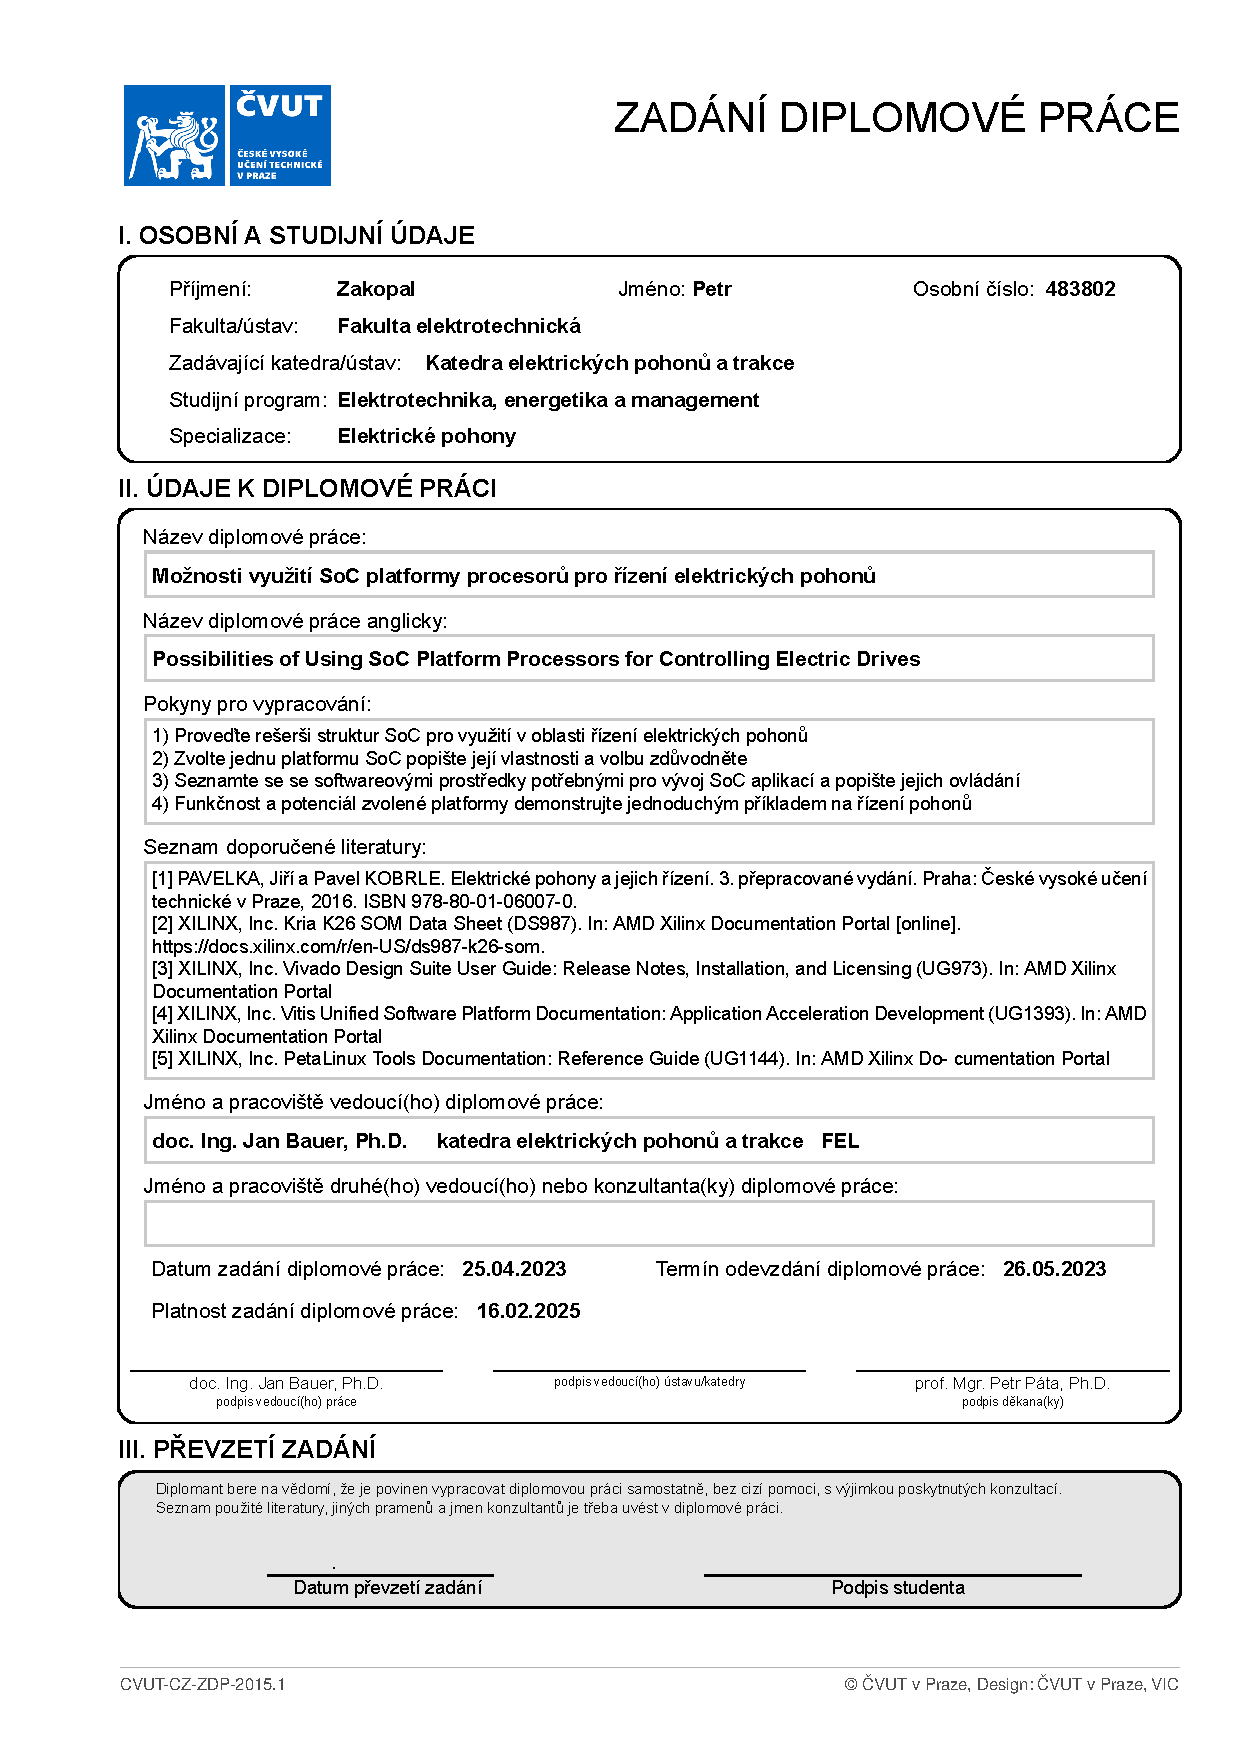
\includepdf[]{src/docs/zadani_bez_podpisu.pdf}

%\newpage
%\cleardoublepage
\null\newpage

\pagenumbering{Roman}
\setcounter{page}{5}%%3 NUTNO řešit dle zadání etc.

\noindent \textcolor{ctublue}{{\Large{\textbf{\MakeTextUppercase{Prohlášení}}}}}\\
			Prohlašuji, že jsem předloženou práci vypracoval samostatně a že jsem uvedl veškeré použité informační zdroje v~souladu s~Metodickým pokynem o~dodržování etických principů při přípravě vysokoškolských závěrečných prací.\\
		\vspace{1.5cm}
		
	

	\noindent	V~Praze dne \rule{3.5cm}{0.4pt} \hspace{6.6cm}  \rule{4cm}{0.4pt}
	
	\hspace{12.65cm}Petr Zakopal


		\vspace{14cm}
		
	\noindent	\textcolor{ctublue}{{\Large{\textbf{\MakeTextUppercase{Poděkování}}}}}\\
	Nam quis commodo justo. Mauris diam metus, mattis sed rutrum in, volutpat sit amet sem. Nam bibendum commodo porttitor. Quisque eget lectus rutrum, molestie tortor id, iaculis nunc. Sed et maximus ipsum. Vivamus vel facilisis nisl. Curabitur eu nibh nec erat mollis finibus at in sapien. Mauris viverra sapien neque, nec lacinia odio laoreet eu. Quisque consectetur eros ac orci interdum scelerisque.
		


%%ABSTRAKT%%

\newpage
%\addcontentsline{toc}{section}{3\quad Abstrakt a klíčová slova}%Added citations to TOC%
%\begin{comment}
\begin{minipage}[t]{7.37cm}
		%\raggedright
	\textcolor{ctublue}{\Large{\textbf{\MakeTextUppercase{Abstrakt}}}}\\
	Nam quis commodo justo. Mauris diam metus, mattis sed rutrum in, volutpat sit amet sem. Nam bibendum commodo porttitor. Quisque eget lectus rutrum, molestie tortor id, iaculis nunc. Sed et maximus ipsum. Vivamus vel facilisis nisl. Curabitur eu nibh nec erat mollis finibus at in sapien. Mauris viverra sapien neque, nec lacinia odio laoreet eu. Quisque consectetur eros ac orci interdum scelerisque.\\
	\textbf{Klíčová slova:} Lorem ipsum dolor sit amet, consectetur adipiscing elit. Duis aliquam finibus sagittis. Nunc venenatis, augue quis luctus dictum, elit justo pharetra leo, nec viverra purus dui at quam.
\end{minipage}%
\hfill% --- important, otherwise it wont be so nice
\begin{minipage}[t]{7.37cm}
		\textcolor{ctublue}{\Large{\textbf{\MakeTextUppercase{Abstract}}}}\\
		Nam quis commodo justo. Mauris diam metus, mattis sed rutrum in, volutpat sit amet sem. Nam bibendum commodo porttitor. Quisque eget lectus rutrum, molestie tortor id, iaculis nunc. Sed et maximus ipsum. Vivamus vel facilisis nisl. Curabitur eu nibh nec erat mollis finibus at in sapien. Mauris viverra sapien neque, nec lacinia odio laoreet eu. Quisque consectetur eros ac orci interdum scelerisque.\\
		\textbf{Keywords:} Lorem ipsum dolor sit amet, consectetur adipiscing elit. Duis aliquam finibus sagittis. Nunc venenatis, augue quis luctus dictum, elit justo pharetra leo, nec viverra purus dui at quam.
\end{minipage}
%\end{comment}
	%\textcolor{ctublue}{\Large{\textbf{\MakeTextUppercase{Abstrakt}}}}\\

	%\textcolor{ctublue}{\Large{\textbf{\MakeTextUppercase{Abstract}}}}\\

\newpage
\tableofcontents
\newpage%
\flushbottom %vyčištění stránky
\newpage
\vspace{0pt}
\listoffigures %seznam obrázků
\flushbottom %vyčištění stránky
\newpage
\listoftables
\flushbottom
\newpage


\pagenumbering{arabic} %to arabic page numbering - enabling page numbering after gobble which disabled page numbering
\pagenumbering{gobble}
\null\newpage
\null\newpage %PŘI VERZI ONLINE
\setcounter{page}{1}
\pagenumbering{arabic}
\fontspec{Times New Roman}

\section{Úvod}
V~době, kdy byla od elektrických pohonů požadována spolehlivost, vysoká účinnost a nenáročné ovšem kvalitní řízení, byly k~řízení využívány samotné digitální signálové procesory. Postupem času dochází ke zjištění, že výkon DSP není dostatečný a na některé aplikace, kde je vyžadováno provedení značné množství náročných výpočtů za co nejkratší čas, nejsou vhodné. Proto nastupuje éra logických programovatelných polí (FPGA), které jsou schopny tyto výpočty provést s~velmi nízkými nároky na energii a za velmi krátký čas.\par
V~mnoha odvětvích se již začíná využívat embedded systém s~Application Spefified Hardware, který je určen pouze na využití v~předem dané aplikaci. Tento hardware slouží v~dané aplikaci k~jedinému účelu, který vykonává a na který je optimalizován. Tím se liší od procesoru, který vykonává mnoho instrukcí a využít ho pouze jako samostatnou výpočetní jednotku je z~hlediska energetické i finanční náročnosti nevýhodné. Implementace hradlových polí přináší nejen v~řízení elektrických pohonů zvýšení výpočetního výkonu, ale také snižování energetické náročnosti řízení.\par
Perspektiva logických programovatelných polí a hardwaerově urychlovaných aplikací je podpořena jejich využíváním i mimo obor elektrických pohonů a trakce. Z~důvodu jejich veliké propustnosti, vysokých výpočetních výkonů a nízké energetické náročnosti jsou využívány v~AI, machine learningu, zpracování obrazu, těžení kryptoměn a jiných nepohonářských aplikacích.\par
Nevýhodou problematiky FPGA je jejich složitější programovatelnost z~hlediska tvoření aplikace. Aplikace je tvořena určitým postupem (workflow), který kladne vysoké nároky na vzdělání a zkušenosti vývojářů. Většina FPGA je programována pomocí jazyků Verilog či VHDL, které mohou pro softwarově orientované programátory představovat značnou překážku. Proto bylo vyvinuto tvoření aplikací pomocí vyšší úrovně syntézy (HLS), kdy je možné tvořit programy ve vyšších programovacích jazycích jako je například C, C++ či Python. HLS umožnilo rapidní rozšíření a využití Embedded FPGA Accelerated Applications v~mnoha aplikacích a značně vylepšilo vývojářský požitek (developer experience, DX) při tvorbě aplikací.\par
Protože může být náročné vytvořit vlastní architekturu, složenou z~CPU a spolupracujícího FPGA, je vhodné při prvotním vývoji aplikace využít dostupné vývojové desky obsahující již předpřipravené propojení jednotlivých komponent. Součástí těchto vývojových desek bývá také mnoho vstupů a výstupů (I/O) pro snadnější využití při lazení a tvoření aplikace. V~této práci je využívána vývojová deska Zybo od firmy Digilent. Ovšem autor v~textu představuje další možnosti, které mohou být pro konkrétní aplikace a využití vhodnější.\par
Tato práce se zajímá o~aplikace a možné využití FPGA při řízení elektrických pohonů. Autor v~ní představuje základní principy Hardware Accelerated Applications, z~jakého důvodu je tento přístup perspektivní a proč je vhodné se orientovat tímto směrem.\par
\flushbottom %vyčištění stránky
\newpage
%konec úvodu

\section{System on a chip}\label{sec:system-on-a-chip}
	% co to je, proč to je
	% typy postavené kolem  mikrokontroléru, mikroprocesoru a ASIC
	% Aplikace Embedded system (existují i pro mobilní aplikace, osobní počítače)
	System on a chip (SoC) je architektura čipu, využívající takovou konstrukci, kdy jsou integrovány různé části/bloky systému na jeden čip. Integrace prvků na jeden čip značně snižuje nároky na rozměry nosičů, na kterých jsou tyto SoC umístěny. Místo diskrétních čipů, obstarávající jednotlivé funkce, je využito jednoho čipu s~mnoha částmi vykonávající požadované funkce.\par
	Protože integrování čipů do jedné polovodičové struktury představuje relativně veliké snížení nároků na kovové vodivé spoje a snižuje časovou náročnost a zvyšuje rychlost přenosu dat, je SoC upřednostňováno před metalicky spojenými diskrétními částmi vykonávající dané operace.\par
	Označení SoC může představovat mnoho architektur. Obecné rozdělení, nalezitelné v~literatuře a veřejných zdrojích, těchto architektur je následující:
	\begin{itemize}
		\item SoC využívající mikrokontroléru (CPU, RAM, ROM),
		\item SoC využívající pouze mikroprocesoru (CPU, možné i GPU, jádra pro specializované výpočty),
		\item SoC pro specifické aplikace (Application Specific Integrated Circuit – ASIC).
	\end{itemize}
	Jedná se tudíž o~rozdělení dle hlavní výpočetní jednotky, resp. procesoru v~čipu. \cite{tomshardware-system-on-chip}\par
	Z~uvedených rozdělení jsou pro řízení elektrických pohonů nejvíce využívány SoC s~mikrokontrolérem a ASIC.

	\subsection{Application Specific Integrated Circuit}
		Významnou část SoC tvoří \textit{Application Specific Integrated Circuits, popř. Hardware} (ASICs, ASHW). Při použití těchto SoC je využíváno přesvědčení, že pokud je architektura HW přímo specializovaná na jednu aplikaci, je vysoká pravděpodobnost, že ji bude vykonávat bezchybně, kvalitně a rychle.\par
		Tyto aplikace jsou využívány v~širokém spektru oborů jako je např. zpracování zvuku, videa, výpočtů apod. Tyto ASIC mohou také vykonávat potřebné rychlé výpočty pro matematické modely elektrických strojů, které jsou využívány např. pro HIL.\par
		Než je tento specifický obvod vytvořen, je nutné jej navrhnout, vyzkoušet a odladit. K~tomu slouží logická programovatelná pole, ve kterých je možné požadovaný HW navrhnut a odladit před velko produkcí ASIC. Pokud velko produkce není z~ekonomických důvodů možná, jsou FPGA využívány přímo v~produkci s~jejichž pomocí je vytvořena HW struktura, která by byla přítomna na ASIC.


	\subsection{Aplikace SoC}
	Systémy na čipu se pro jejich výpočetní výkon, prostorovou a energetickou efektivnost využívají v~mnoha aplikacích. Nejvýznamnější využití v~problematice elektrických pohonů je v~embedded systémech a hardwaerově akcelerovaných aplikacích.

\section{System on Modules}\label{sec:system-on-modules}

	System on modules (SOMs) je architektura jejíž jednou z~hlavních součástí je dříve zmiňovaný SoC. SOMs se oproti SoC již dodávají na PCB a kromě SoC mají na desce umístěné další komponenty, které jsou pro danou aplikaci vyžadovány. \cite{xilinx-what-is-a-som}\par
	SOMs se mohou dodávat jako vývojové desky \cite{xilinx-kria-kr260-robotics-starter-kit}, které obsahují krom SOM taktéž podpůrnou desku s~dalšími obecnými komponenty, jež jsou vhodné pro vývoj standardních aplikací. Pokud zákazník již pomocí vývojové desky odladil vytvářenou aplikaci, může zakoupit samostatný SOM na base board (BB) a podpůrnou desku (tzv. carrier card, CC) pro danou aplikaci navrhnou tak, aby obsahovala pouze komponenty, které daná aplikace využívá. Tudíž se snižuje cena konečného výrobku o~komponenty, které byly z~carrier card při návrhu odstraněny pro jejich nevyužití.\par
	Výrobce platformy \textit{Kria KR260 Robotics Starter Kit}, použité v~této práci, dodává k~produktu rozsáhlou dokumentaci \cite{kria-som-carrier-card-design-guide-2022} \cite{kria-k26-som-ds}, podle které je možné individuální carrier card sestavit. \par
	Příkladem individuálně vytvořené carrier card je open source projekt od firmy \textit{Antmicro Ltd}. Tato firma vydala open source design carrier cardu pro zařízení \textit{Kria K26}, které je předchůdcem \textit{KR260}, a bylo určeno pro akcelerování audiovizuálních aplikací. Využívá však totožný SOM ale rozdílný carrier card. Dokumentace a vytvořený návrh je dostupný z~\cite{antmicro-open-source-kria-k26-carrier-card}.

	\subsubsection{Embedded Systems}
	Embedded systéms je název pro skupinu zařízení, obecně systémů, které je možné charakterizovat jako specifické výpočetní zařízení, resp. počítače, které jsou určeny pro podporu funkce nebo řízení nějakého většího celku, produktu nebo fyzikálního systému. Oproti tomu osobní počítač je sice výpočetní zařízení, ale nelze mluvit o~embedded systému, protože je určen pro mnoho univerzálních aplikací. \cite{Sass2010}\par
	Dalším důležitým rozdílem mezi \textit{Embedded System} a obecným výpočetním zařízením je ten, že v~případě embedded systému je interakce mezi systémem a uživatelem uměle omezena na základní ovládání či kontrolu funkce. Není předpokládáno, že by uživatel, jež aplikaci embedded systému využvá, výrazným způsobem zasahoval do jeho funkce. Naopak obecný výpočetní systém je uzpůsoben na podstatné zásahy uživatele. \cite{Sass2010} \cite{juan-fpgas}\par
	Do embedded systému vstupují signály, které jsou následně zpracovány a poté vybrané výsledky výpočtů jsou v~podobě výstupní signálů výstupním produktem systému. Tyto produkty mohou pomocí akčních členů zasahovat do řízeného systému. Vstupní signály většinou přicházejí ze speciálních snímačů, kompatibilních s~embedded systémem (senzor teploty, senzor tlaku, senzor zrychlení, gyroskop, senzory proudu, inkrementální čidla apod.). Naopak jeho výstupní signály jsou například specifická ovládací hodnota napětí, proudu nebo jiné veličiny. Také mohou být na výstupních pinech připojené LED signalizace, komunikační sběrnice některých komunikačních systémů nebo výstupní LDC displaye. Způsob, kterým jsou kódovány vstupní a výstupní signály, je většinou specificky určený daným řízeným systémem. \cite{Sass2010}\par
	K~obecnému výpočetnímu systému je možné připojit vstupní periferie klasických osbních počítačů – myš, klávesnice, mikrofon. Komunikace embedded systému s~periferiemi je většinou standardizována tak, aby bylo možné periferie libovolně zaměňovat bez změny funkčnosti. \cite{Sass2010}.\par
	Na obrázku \ref{fig:embedded-system-scheme} je zobrazeno názorné blokové schéma řízení fyzikálního systému pomocí embedded systému. Tyto bloky mezi sebou komunikují pomocí digitálních signálů. Pokud tyto signály nejsou digitální, musí se před zpracováním v~embedded systému zdiskretizovat.

	\begin{figure}[htbp!]
		\centering
			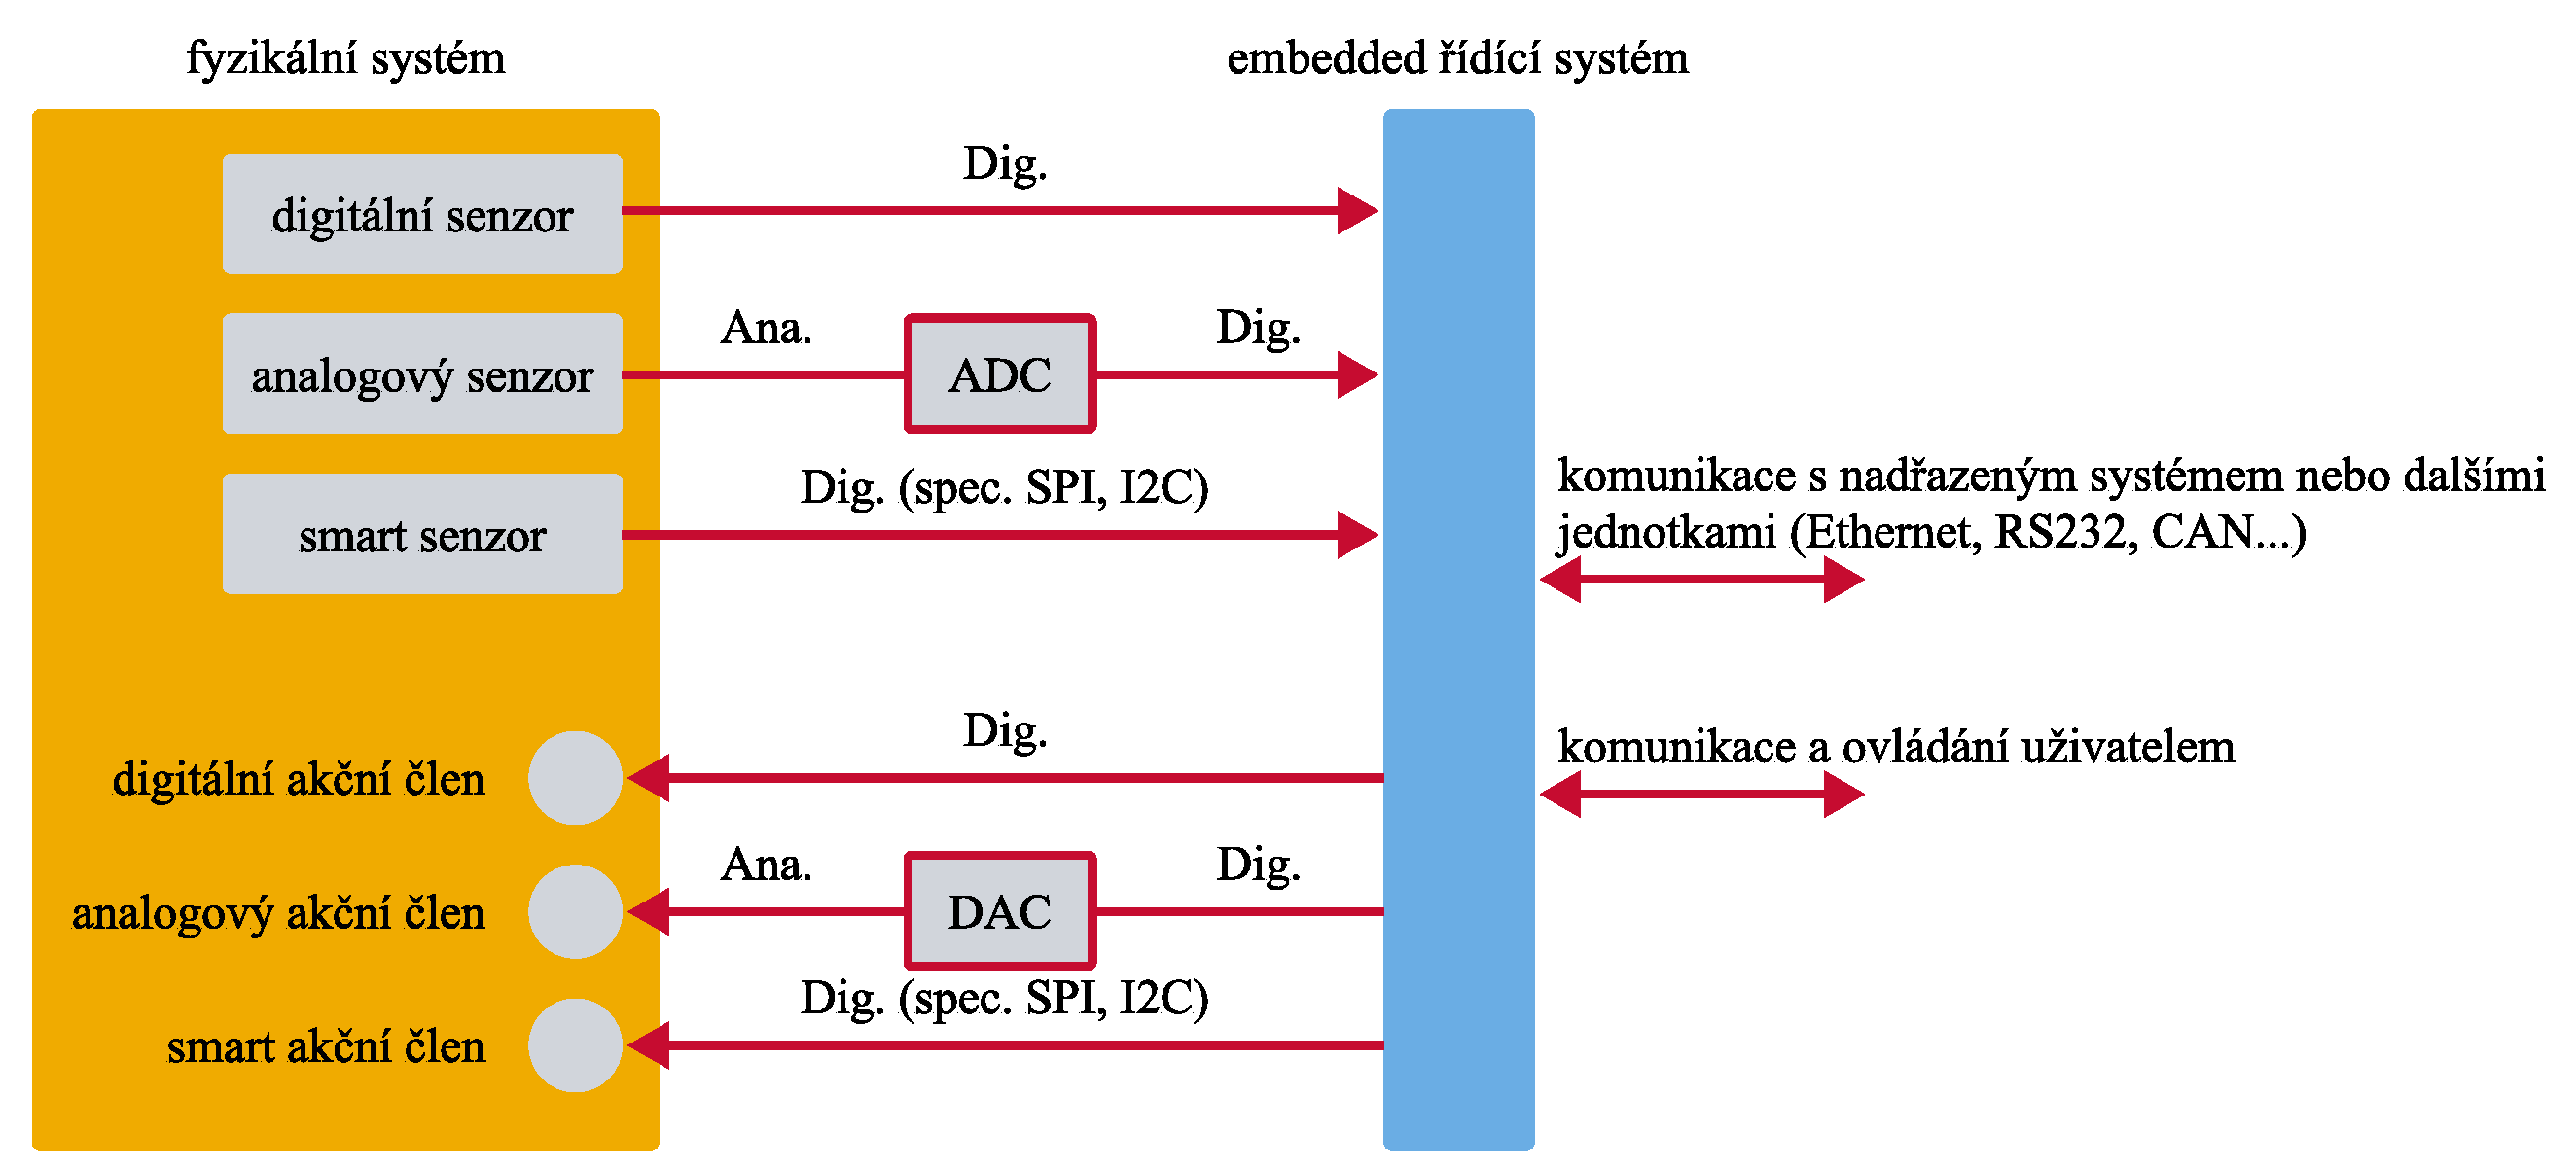
\includegraphics[width=1\textwidth]{src/pdf/embedded-system-scheme.pdf} 
			\caption{Blokové schéma Embedded systému a řízeného fyzikálního systému. (převzato a upraveno z~\cite{juan-fpgas})}
			\label{fig:embedded-system-scheme}
	\end{figure}

		\fbar

		\subsubsection{Hardware Accelerated Applications}\label{subsec:hardware-accelerated-applications}
		V~mnoha aplikacích, nejen při řízení elektrických pohonů, je vyžadováno, aby výpočty nebo zpracování dat probíhalo vysokou rychlostí. Tento problém nemůže být většinou vyřešen použitím běžného procesoru (CPU), který je optimalizován na provádění obecných komplexních funkcí, řízení běhu uživatelského programu, komunikaci či přesun dat. V~moderním světě je třeba zpracovávat exponenciálně narrůstající množství dat. Aby tyto data bylo možné v~požadovaném čase, s~co nejnižším zpožděním zpracovat, je vhodné využít specifický HW a přístup, který bude schopen požadavky rychlosti a výkonu uspokojit. Tento přístup se nazývá \textit{Hardware Acceleration} (hardwaerová akcelerace). \cite{xilinx-accelerated-computing}\par
		Princip hardwaerové akcelerace spočívá v~přesunu výpočetně náročných aktivit na specifický a oddělený hardware. Celkové řízení běhu aplikace a komunikace je ovšem stále vykonáváno řídícím CPU. Oddělený hardware, na kterém dochází k~akceleraci výpočtů, je optimalizován na vykonávanou úlohu a jeho využití přináší zefektivnění běhu celkové aplikace. \cite{xilinx-accelerated-computing}\par
		Struktura, ve které je využíváno více fyzicky oddělených procesorových a hardwaerových akceleračních jednotek, se často nazývá heterogenní. \cite{xilinx-accelerated-computing}\par
		Hardwaerová akcelerace poskytuje rychlejší výpočty než CPU, protože využívá maximální paralelizace výpočtů. Klasické CPU však vykonává jednotlivé instrukce sériově. I~v~případě, že CPU má více jader a využívá více vláken, nemůže se specifické úrovni paralelismu při dané omezující energetické náročnosti HW vyrovnat.
		Pro HW akceleraci je v~mnoha oblastech využíváno několik druhů jednotek, které jsou optimální pro dané aplikace.\par
		\textbf{Graphics Processing Units} (GPUs) jsou jednotky, které převážně slouží k~akceleraci zpracování vizuálních úloh. V~době rapidního rozvoje elektroniky a SW je možné využití GPUs v~mnoha odvětví umělé inteligence (AI) či kreativních odvětích. GPUs jsou využívány v~aplikacích, kde není kladen veliký důraz na nízkou odezvu (latenci). \cite{xilinx-accelerated-computing}\par
		\textbf{Tensor Processing Units} (TPUs) jsou jednotky, které slouží k~provádění algoritmů strojového učení (machine-learning, ML). Jejich přímé datové propojení umožňuje velmi rychlý a přímý přenost dat. Díky přímému připojení nevyžadují využití pamětí, které by přenos dat zpomalovaly. \cite{xilinx-accelerated-computing}\par
		\textbf{Field Programmable Gate Arrays} (FPGAs) jsou jednotky, ve kterých není při výrobě pevně daná HW struktura. To umožňuje vytvoření, resp. naprogramování HW dle požadavků akcelerované aplikace. FPGAs mohou být využívány i při výpočtech v~reálném čase matematických modelů elektrických strojů. Při realizaci této práce je pro akceleraci využíváno právě těchto programovatelných polí.\\ \\
		\noindent Porovnání časové náročnosti matematických výpočtů pro selektivní eliminaci harmonických složek v~trakci pomocí CPU a GPU (graphics processing unit) je provedeno v~\cite{ieee-selective-harmonic-elimination-nvidia}.\par
		Z~článku vyplývá že využitím GPU skutečně dochází k~snížení potřebného času na představený výpočet. V~některých případech se jedná o~snížení výpočetního času z~183 ms (při použití CPU) na 0,81 ms (při použití NVIDIA Titan V~GPU). Díky využití GPU je tedy možné algoritmus provádět v~reálném čase v~lokomotivě.

	\subsubsection{Výpočetní technika, mobilní zařízení a elektronika}
	Kromě průmyslových odvětví jsou SoC využívány i pro běžné aplikace spotřební elektroniky.\par
	Protože jsou kladeny stále vyšší nároky na výpočetní rychlost a nižší cenu ve spotřební elektronice, jako jsou mobilní zařízení (mobilní telefony, osobní počítače), servery apod., začíná převažovat využívání SoC i v~těchto oblastech.\par
	Společnost Apple Inc. již téměř ve všech vlastních novějších zařízeních používá individuálně navrhnutý SoC.\par
	Příkladem je A16 Bionic pro iPhone 14 Pro, Apple M1 a M2 pro tablety a počítače.\par
	Díky specifickým řešením a vylepšeným architekturám (jádra SoC pro vysoký výkon a jádra pro ekonomickou spotřebu energie) bylo možné značně zvýšit výkon a snížit energetickou náročnost zařízení spotřební elektroniky. \cite{apple-explore-the-new-architecture-of-apple-silicon-macs}


	\section{Programovatelné hradlové pole – FPGA}
		\subsection{Vývoj FPGA z~PLD}
		Programovatelné hradlové pole jsou zařízení, jejichž historický vývoj stojí na programovatelných logických zařízení (programmable logic devices, PLD). První PLD fungovala na principu Booleových funkcí součtu násobení (sum of products). Tato zařízení obsahovala matici (proto se také nazývají programmable logic arrays, PLA) více vstupových bloků AND a OR. Programování požadované funkce probíhalo pomocí přerušování vstupů do jednotlivých logických bloků. Později byly do PLA přidány D klopné obvody s~multiplexory. Díky těmto součástím bylo možné vytvářet logické kombinační a sekvenční obvody, resp. automaty. Posledním vylepšením PLA, které stálo před zrodem FPGA, spočívalo v~umístění více PLA bloků (skládajících se z~AND, OR, multiplexeru a D klopného obvodu) na jeden integrovaný čip. Programovatelné spojení různých PLA bloků a výstupů umožnilo vytvořit požadovanou funkci. \cite{Sass2010}\par

		\subsection{Aktuální složení FPGA}
		Moderní FPGA se skládají z~2D matice propojených programovatelných logických bloků, bloků speciálních funkcí a propojů vytvořených pomocí CMOS technologie. Po obvodě FPGA jsou rozmístěny vstupní a výstupní piny (I/O), připojené na zvláštní logické bloky. Použité logické bloky se skládají z~mnoha buněk, které se skládají z~generátorů funkcí a paměťových elementů. \cite{Sass2010}\par
		Na obr. \ref{fig:fpga-general-design} je možné pozorovat názorné schéma základního konceptu uspořádání FPGA. Na schématu jsou vyznačeny logické bloky, jejich propojení, propojovací matice pro aktivování jednotlivých propojů a vstupů a výstupů (I/O) FPGA.\par
		I~přesto, že se tato práce převážně věnuje využití SoC a SOM pro řízení elektrických pohonů je vhodné představit základní části FPGA a nastínit jejich funkci.

		\begin{figure}[htbp!]
			\centering
				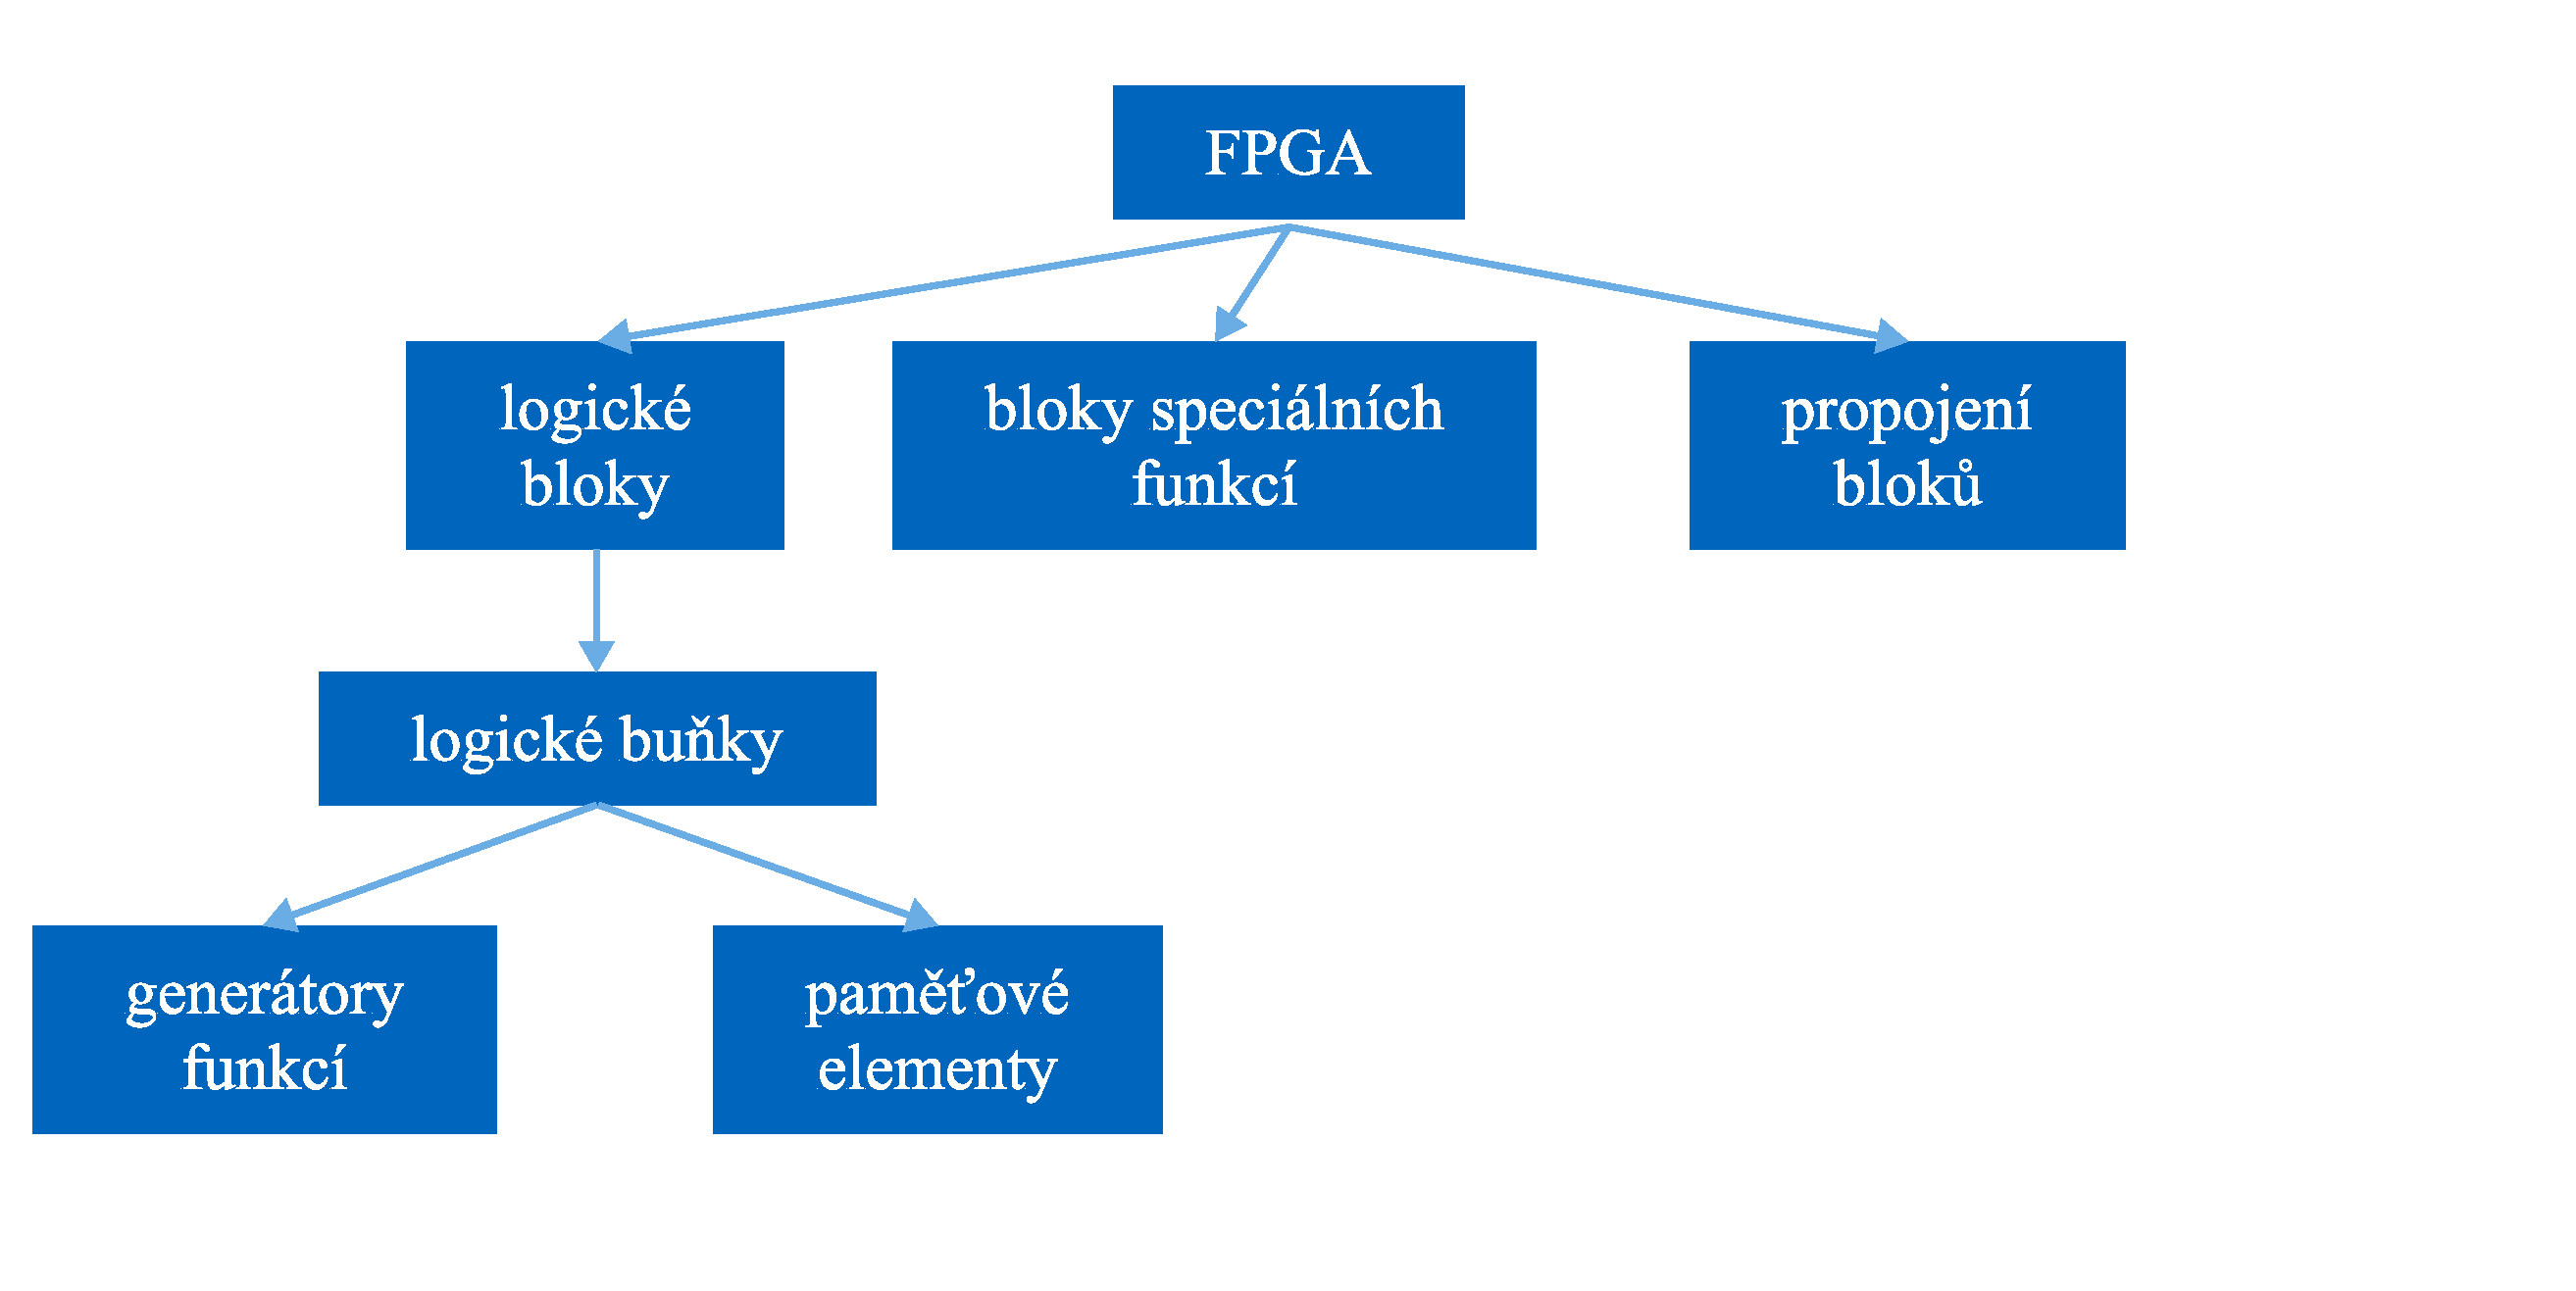
\includegraphics[width=1\textwidth]{src/pdf/fpga-skladba.pdf} 
				\caption{Blokové schéma složení moderních FPGA.}
				\label{fig:fpga-skladba}
		\end{figure}


		\begin{figure}[htbp!]
			\centering
				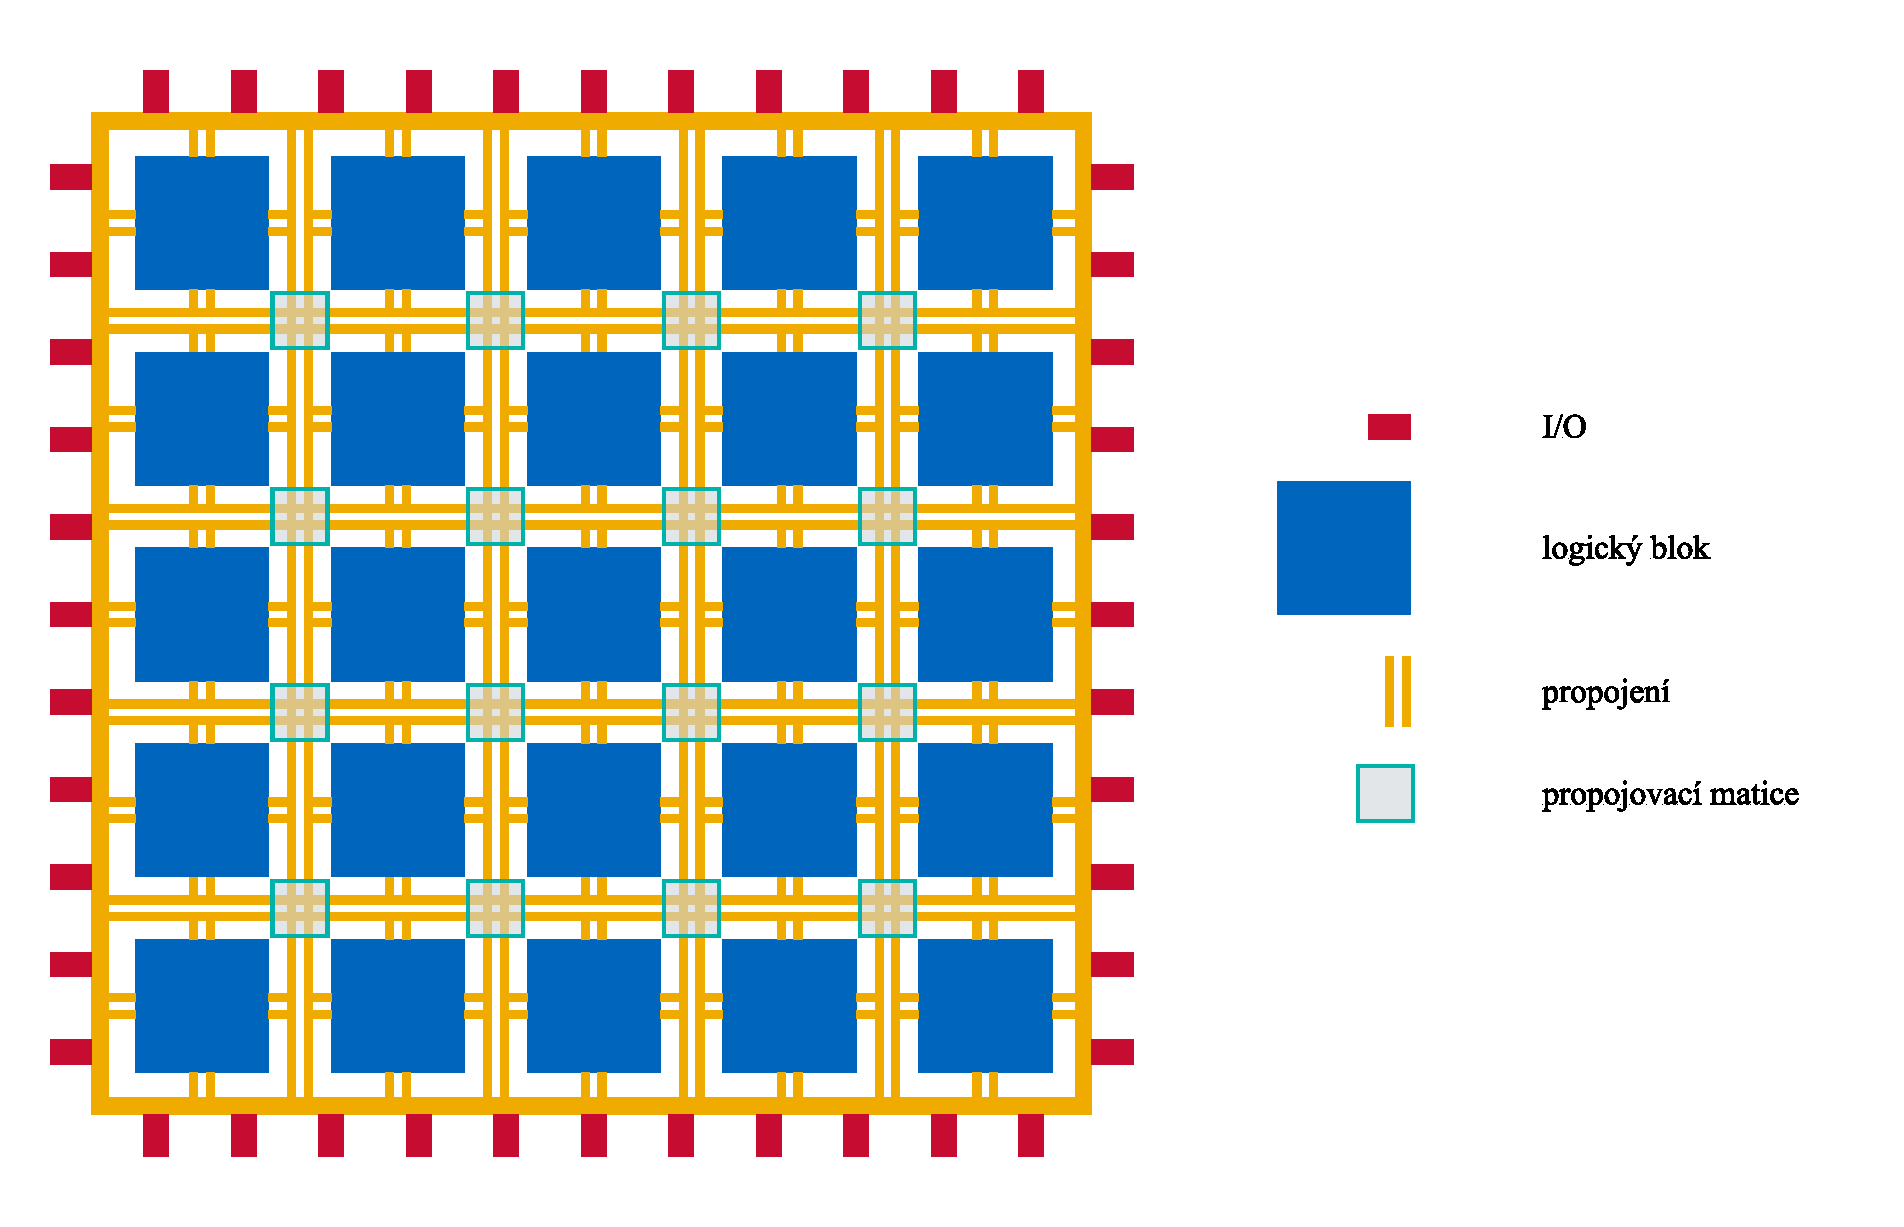
\includegraphics[width=1\textwidth]{src/pdf/fpga-general-design.pdf} 
				\caption{Základní koncept uspořádání FPGA.}
				\label{fig:fpga-general-design}
		\end{figure}

		\fbar
		\subsubsection{Generátory funkcí}\label{subsubsec:generatory-funkci}
		Oproti předchůdcům (PLD), které pro generování funkcí používaly logická hradla tvořená CMOS tranzistory, využívají FPGA generátory funkcí.\par
		Logickou funkci je možné popsat pravdivostní tabulkou, která má určitý počet vstupů a odpovídající počet výstupů. Dle \cite{Sass2010} je možné si představit, že se generátor dané funkce skládá ze samostatné statické paměti (SRAM), jejíž výstupy jsou přímo přivedeny na vstup multiplexeru (MUX). Signály výběru výstupů by odpovídaly vstupním proměnným a jednotlivé vstupy do MUX výstupům funkce.\par
		Pro bližší pochopení funkce generátoru funkcí z~předchozího odstavce je možné představit realizaci smyšlené logické funkce $\text{f} (x, y, z) = \bar{x}z + y$. Pravdivostní tabulka této smyšlené logické funkce je zobrazena v~tab. \ref{tab:fpga-pravdivostni-tabulka-smyslene-funkce-generatoru-funkci}. Odpovídající realizace pomocí MUX a SRAM je zobrazena na obr. \ref{fig:fpga-function-generator}. Tato reprezentace se nazývá look-up table (LUT). Grafické znázornění inspirováno \cite{Sass2010}.
		

	\begin{minipage}[t]{0.45\textwidth}
		\begin{table}[H]
			\centering
			\caption{Pravdivostní tabulka ukázkové funkce, realizované v~generátoru funkcí, umístěném v~logickém bloku FPGA.}
		  \vspace*{0.15cm}
		
			\begin{tabular}{!{\vrule width 2pt} c | c | c | c !{\vrule width 2pt} c !{\vrule width 2pt}}
			\noalign{\hrule height 2pt}
			$i$ & $x$ &	$y$ & $z$ & f($x,y,z$)\\
			\noalign{\hrule height 2pt}
			0 & 0 & 0 & 0 & 0\\ \hline
			1 & 0 & 0 & 1 & 1\\ \hline
			2 & 0 & 1 & 0 & 1\\ \hline
			3 & 0 & 1 & 1 & 1\\ \hline
			4 & 1 & 0 & 0 & 0\\ \hline
			5 & 1 & 0 & 1 & 0\\ \hline
			6 & 1 & 1 & 0 & 1\\ \hline
			7 & 1 & 1 & 1 & 1\\\noalign{\hrule height 2pt}
			\end{tabular}
			\label{tab:fpga-pravdivostni-tabulka-smyslene-funkce-generatoru-funkci}
		\end{table}
	\end{minipage}%
	\hfill% --- important, otherwise it wont be so nice
	\begin{minipage}[t]{0.45\textwidth}
		\begin{figure}[H]
			\centering
				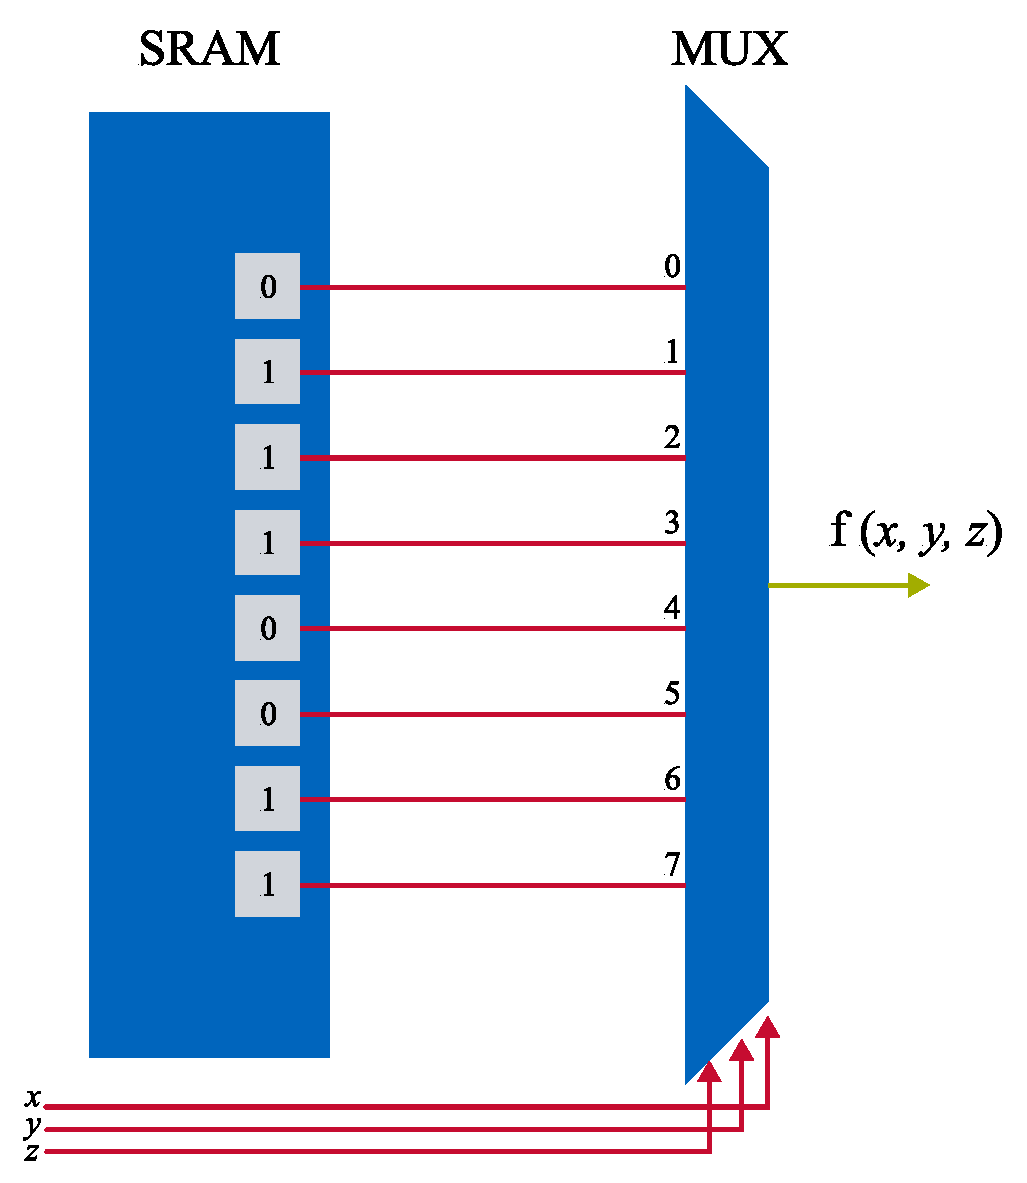
\includegraphics[width=1\textwidth]{src/pdf/fpga-function-generator.pdf} 
				\caption{Ukázka, jakým způsobem realizuje funkční generátor požadovanou funkci pomocí SRAM a MUX.}
				\label{fig:fpga-function-generator}
		\end{figure}
	\end{minipage}

	\vspace*{0.5cm}
	Výhoda této reprezentace funkcí oproti logickým hradlům je, že doba zpoždění signálu (propagation delay) pro funkci je konstantní. Respektivě je konstantní, pokud funkci je možné realizovat jednou LUT. Pro relizace obecné funkce je zapotřebí multiplexer $2^{n}$ -> 1 a SRAM s~počtem buněk $2^{n}$, kde $n$ je počet vstupních proměnných dané funkce. \cite{Sass2010}

	\subsubsection{Paměťové elementy}\label{subsubsec:pametove-elementy}
		Paměťové elementy jsou v~FPGA realizovány pomocí D-klopných obvodů. Tyto obvody mohou při konfiguraci FPGA být nastaveny, že budou reagovat na nástupnou nebo sestupnou hranu časovacího signálu (clock, CLK) řídícího procesoru nebo na úroveň řídícího signálu (latch).\cite{Sass2010}\par
		Protože typ latch je citlivý na úroveň signálu, může být problematické dovést požadovaný signál na vstup klopného obvodu v~požadovaném čase. Velmi často jsou proto paměťové členy konfigurovány jako D-klopné obvody reagující na hranu. Pokud je používán signál CLK vyšších frekvencí, je D-klopný obvod reagující na hranu snadněji schopný reagovat v~požadovaném čase. \cite{Sass2010}\par
		Často jsou na vstup paměťových elementů připojeny výstupy multiplexerů \hyperref[subsubsec:generatory-funkci]{\textit{generátorů funkcí}}. \cite{Sass2010}

		\subsubsection{Logické buňky}
			Logické buňky jsou elementy, skládájící se z~\hyperref[subsubsec:generatory-funkci]{\textit{generátorů funkcí}} a \hyperref[subsubsec:pametove-elementy]{\textit{paměťových elementů}}. Velmi často se počet logických buněk údává jako jeden ze základních parametrů FPGA, podle kterého je uživatel možný rozhodnout, zda je vhodný pro jeho aplikaci. Pomocí logické buňky nebo skupiny logických buněk je již možné vytvářet plnohodnotnou kombinační a sekvenčí logiku.\cite{Sass2010}

		\subsubsection{Logické bloky}\label{subsubsec:logicke-bloky}
			Logické bloky se skládají ze spojení několika logických buněk do jedné skupiny. Díky umístění této skupiny buněk na čip geograficky blízko, dochází k~minimalizaci zpoždění signálu mezi jednotlivýmu buňkami. Častá skutečnost je, že jednotlivé bloky mohou mít již předkonfigurovanou funkci, jako je např. sčítačka, dělička nebo násobička. \cite{Sass2010}

		\subsubsection{Propojení bloků}
			Propojení bloků je prováděno ke spojení jednotlivých logických bloků a I/O. Pro spínání určených propojů jsou na čipu mezi jednotlivými propoji umístěny propojovací matice, resp. „přepínače“. Ty slouží ke spojení jinak oddělených propojů, logických bloků a I/O. \cite{Sass2010}
			Na obr. \ref{fig:fpga-skladba} je prezentována 2D struktura pole. Ovšem pro zvětšení počtu LUTs, tudíž výpočetního výkonu, a snížení vzdáleností mezi logickými bloky je v~moderních FPGA použita 3D struktura, kdy dochá k~vrstvení jednotlivých logických bloků a jejich propojů do výšky. \cite{pang-beginning-fpga}

		\subsubsection{I/O bloky}
				I/O bloky jsou obvykle umístěny na okraji designu FPGA. Slouží k~přivedení resp. vyvedení signálů FPGA na externí připojovací piny struktury. Tyto výstupní bloky mohou využívat různé standardy k~přenosu informací typu \textit{single-ended} (napětí vztaženo k~referenční nule) (LVTTL, LVCMOS PCI, PCIe, SSTL) nebo typu \textit{double data rate} (diferenciální signál, vztažený k~výstupu jiného I/O bloku) (LVDS). I/O bloky jsou strategicky umístěny na okraj struktury, aby byla minimalizována vzdálenost mezi I/O blokem a hranicí FPGA, představující vnější okolí. \cite{Sass2010} \cite{pang-beginning-fpga}

		\subsubsection{Bloky speciálních funkcí}
			Aby došlo např. ke zvýšeení rychlosti přenosu dat z~FPGA do externího CPU a naopak, jsou některé speciální funkce implementovány jako funkční bloky přímo do struktury FPGA. To umožňuje efektivní využití FPGA pro různorodé aplikace. \cite{Sass2010}\par
			\textbf{Block RAM} (BRAM) je blok, který slouží k~uchování dat. Sice by bylo možné vytvořit paměťový blok z~\hyperref[subsubsec:logicke-bloky]{\textit{Logických bloků}}, ale docházelo by k~omezení využití FPGA pro jeho původní aplikaci a pro realizaci by bylo potřeba využít mnoho bloků. BRAM mají oddělený vstup a výstup, současně s~odděleným CLK. Proto je možné do BRAM zároveň data zapisovat a zároveň z~něj číst. \cite{Sass2010}\par
			\textbf{DSP}, resp. digital signal processing bloky slouží ke zpracování digitálního signálu. V~těchto blocích jsou implementované funkce AND, OR, NAND, NOT, násobičky a sčítačky. Mají nízkou spotřebu. DSP bloky jsou často umístěny geograficky blízko bloků BRAM, které slouží jako „mezipaměti“ (buffer). \cite{Sass2010}\par
			\textbf{Procesor} implementovaný do struktury FPGA snižuje časové zpoždění při obsluhování FPGA. \cite{Sass2010}\par
			\textbf{Digital Clock Manager} slouží k~vytvoření jiného, resp. nižšího taktovacího signálu CLK, který je odvozen z~původního vstupního/zdrojového CLK, pro různé bloky v~FPGA. \cite{Sass2010}\par
			\textbf{Multi-Gigabit Transcievers} slouží k~přenosu dat takovým způsobem, aby došlo k~minimalizaci vlivu ručení na přenášená data. Obecně obstarávají optimální serializaci a paralelizaci dat. \cite{Sass2010}\par
			Struktura FPGA, která je obsauje všechny zdroje a funkcionalitu potřebné pro kompletní realizaci aplikace, se nazývá \textit{platform FPGA}.
		\subsection{Programování}
			Ve skutečnosti není možné mluvit o~programování FPGA jako o~klasickém programování mikroprocesorů. Při tvorbě „programu“ pro FPGA dochází k~vytváření struktury, jež bude následně v~FPGA vytvořena. Ovšem z~praktických důvodů se v~praxi využivá pojem „programovat FPGA“.
		\subsubsection{Forma tvorby algoritmu pro FPGA}\label{subsubsec:forma-tvorby-algoritmu-pro-fpga}
		K~programování, resp. konfiguraci FPGA je možné přistupovat z~několika úrovní. Jednou z~využívaných metod popisu požadovaného HW na FPGA je popis struktury/toku signálu obvody (structural/data flow circuits). K~tomuto popisu je využíváno jazyků HDL, VHDL a Verilog (Hardware Description Language, VSIC HDL). V~těchto jazycích je využíváno logických členů AND, OR, NOT nebo bloků sčítaček a násobiček. Forma popisu, jež naopak využívá vyššího programovacího jazyka než HDL je nazývána metoda popisu chování obvodů (behavioral circuits). Zatímco HDL slouží k~popisu hardware s~využitím nízké míry abstrakce, popis ve vyšších programovacích jazycích, které popis pomocí behavioral circuits umožňuje, je pro programátory (zejména ty softwaerové) značně příjemnější, protože využívá běžných procedurálních programovacích jazyků jako je C, C++ nebo Python. Tyto jazyky jsou následně přeloženy/kompilovány do HDL. Po překladu do HDL pomocí \textit{high level synthesis} (HLS) jsou provedeny kroky \textit{synthesis} (syntéza), \textit{place-and-route} (umístění-a-pospojování) a \textit{bitgen} (generace bitstreamu). \cite{Sass2010}\par
		Při použití HLS může vzniknout situace, že bude vytvořen algoritmus, který bude takovým způsobem komplexní, že ho nebude možné syntetizovat na FPGA. Oproti tomu při použití popisu pomocí structural/data flow circuits, je prakticky vždy algoritmus syntetizovatelný. \cite{Sass2010}\par
		Dalším negativním jevem je vytvoření neoptimalizovaného komplexního algoritmu, který se ve vyšším programovacím jazyce jeví jako jednoduchý, ale při překladu do HDL a následných kroků \textit{synthesis -> place-and-route -> bitgen} nebude možné vytvářený HW design do FPGA umístit, protože bude vyžadovat více \textit{resources} (zdrojů LUTs, BRAM, atd.), než je v~zařízení dostupných.\par
		V~praxi je k~tvorbě algoritmů často využíváno vyšších programovacích jazyků a HLS, protože je tento přístup pro značný počet vývojářů SW srozumitelnější. Dalším častým přístupem v~praxi je použití specializovaných SW jako je MATLAB™️ a Simulink, které jsou schopny při použití odpovídajících balíčků přeložit vytvořený algoritmus do HDL, který je poté možné dále zpracovat a použít pro konfiguraci FPGA. Ovšem využití přístupu se SW MATLAB™️ je třeba disponovat podporovaným HW, který disponuje dostatečným počtem zdrojů v~FPGA struktuře. Tento přístup je značně finančně náročný v~ohledu licence SW a taktéž vlivem vyšší ceny HW s~větším počtem zdrojů.

		\subsubsection{Konverze HDL na konfigurační Bitstream}
			V~části \hyperref[subsubsec:forma-tvorby-algoritmu-pro-fpga]{\textit{Forma tvorby algoritmu pro FPGA}} byly představeny dvě hlavní formy tvorby algoritmu pro FPGA. Aby bylo možné algoritmy na FPGA „umístit“, je třeba vytvořenou rezprezentaci dále zpracovat.\par
			Všechny vyšší úrovně reprezentace algoritmů jsou převedeny na HDL. Následným krokem je \textit{syntéza} (synthesis), která slouží k~převodu HDL na tzv. \textit{netlist}. Při převodu je HDL převáděna na logické členy AND, OR apod. \cite{Sass2010}\par
			Po vytvoření netlistu je nutné rozhodnout, jakým způsobem je možné a výhodné realizovat jednotlivé bloky v~logických buňkách a LUT. Konečné sloučení členů závisí na rozsahu vstupů realizovatelných LUT. Proces seskupování logických členů a určování funkce LUT se nazývá mapování (MAP). Výsledkem MAP je opět netlist. Tento netlist však reprezentuje FPGA členy (LUT, klopné obvody apod.). \cite{Sass2010}\par
			Po mapování následuje proces umisťování (placement) při kterém je rozhodováno které z~logických bloky budou realizovat FPGA členy, získané v~kroku MAP. \cite{Sass2010}\par
			Bloky, které jsou umístěny ve struktuře FPGA je nutné spojit pomocí dostupných propojů na FPGA. Proces spojování a optimalizace propojů takovým způsobem, aby bylo minimalizováno časové zpoždění signálu, se nazývá \textit{routing}. Obvykle se proces slučuje s~MAP do jedné fáze a nazývá se \textit{place-and-route}~(PAR). \cite{Sass2010} \par
			Posledním krokem je vytvoření binárního souboru, nazývaného \textit{bitstream}, který je poté „programováno“ FPGA. Tento proces převede netlist z~kroku PAR na nastavení SRAM v~jednotlivých logických buňkách FPGA tak, aby byl vytvořen požadovaný design v~FPGA. Proces převede konfiguraci propojů a propojovacích matic do SRAM, ovládající příslušné propoje a matice. \cite{Sass2010}\par

			
			\begin{figure}[htbp!]
				\centering
					
\includegraphics[width=1\textwidth]{src/pdf/fpga-hls-to-bitstream-flow-chart.pdf} 
					\caption{Blokové schéma převodu aplikace, naprogramované v~procedurálním jazyce, na bitstream, kterým je konfigurováno FPGA.}
					\label{fig:fpga-hls-to-bitstream-flow-chart}
			\end{figure}

		\fbar
		\subsection{Spotřeba}
			FPGA je využívano pro akceleraci aplikací pro svou nízkou spotřebu energie oproti CPU nebo GPU. Ovšem oproti ASICs FPGA má stále značnější spotřebu, proto je podnikán výzkum, který má za cíl jejich energetickou náročnost snížit ale zachovat jejich výkon a spolehlivost.\par
			% Existuje mnoho článků na téma energy/power efficiency of fpgas ale v žádném není popsáno, proč je jeho spotřeba nižší, než v CPU
			Nižší potřebný výkon pro realizaci nepohonářské aplikace podporuje výzkum a článek \cite{rovere-sphery-vs-shapes}, ve kterém autoři představují svoji práci, v~níž realizovali hru. Ve hře je hlavním úkolem aplikace výpočet stínů a odrazů materiálů. Způsob vykreslení, který je v~aplikaci použit je nazýván \textit{ray tracing}. Ray tracing je označován jako výpočetně náročný způsob, který není vhodný pro on-line aplikace ale pro vykreslování nepohyblivých obrazů, které není nutné zobrazovat v~reálném čase. \cite{wikipedia-ray-tracing}\par
			% píšou jednoho jádra, ale to je divný, spíše prostě spotřeba %
			Autoři v~textu popisují, že v~případě využití FPGA pro výpočty v~reálném čase byla jeho spotřeba 660 mW. Hru autoři vyzkoušeli spustit také na CPU platformě skládající se z~Ryzen™️ 4900H 8-core/16 threads 64-bit CPU @ up to 4,4 GHz clock. V~případš testování na CPU byla indikována spotřeba 33 W. Tudíž při použití FPGA spotřeba klesla přibližně 50x. \cite{rovere-sphery-vs-shapes}.\par
			I~přes nízkou spotřebu energie v~FPGA jsou prováděny výzkumy, jak minimalizovat disipaci elektrické energie v~podobě tepla a přiblížit se tak energetické náročnosti ASICs.\par
			Disipace energie v~FPGA je rozdělena na statickou a dynamickou.\par
			Statická disipace je způsobena zbytkovým proudem tranzistorů ve vypnutém stavu mezi drain a source elektrodou, mezi gate a drain elektrodou a jevem, nazvaným gate direct-tunneling. \cite{grover-reduction-of-power-consumption}\par
			Dynamická disipace je způsobena spínacími a vypínacími ztráty použitých tranzistorů (obvykle CMOS) a je závislá na použitém napětí, frekvenci a kapacitě přechodů, kterou je třeba nabít a vybít při spínání a vypínání tranzistorů. \cite{grover-reduction-of-power-consumption}


			
			\subsection{Využití}
			Programovatelná logická hradlová pole se pro svoji nízkou spotřebu, vysoký výpočetní výkon a klesající cenu elektroniky začínají využívat mnohem častěji v~mnoha odvětví, ve kterých bylo doposavaď využíváno CPU a GPU. Aplikace FPGA je možné v~rámci této práce rozdělit na nepohonářské a pohonářské.

			\subsubsection{Aplikace v~nepohonářských odvětví}
				Díky univerzalitě FPGAs je možné je využít v~mnoha aplikacích různých odvětví. Stále se zvyšující požadavky na výpočetní výkon urychlují nasazování FPGAs do provozů, kde jsou v~současné době instalovány CPU nebo GPU.\par
				Poptávka po dostupnosti FPGA způsobila vznik Cloud služeb, které nabízí FPGA výkon on-demand. Jedním z~velkých poskytovatelů je Amazon Web Services (AWS), který nabízí FPGA akceleraci v~Cloudu. Tuto službu ocení především aplikace, které nejsou vázány na reálný hardware ale pouze potřebují dostupný výpočetní výkon, který mohou v~průběhu tvorby, debuggingu či realizace aplikace měnit bez nutnosti pořizování výkonných a někdy drahých FPGA zařízení. Více o~\textit{Amazon EC2 F1 Instances} služby virtuálních FPGA je dostupné na \cite{amazon-ec2-f1}.\par
				Existuje mnoho výpočetně náročných aplikací jako jsou např. výpočty finančních modelů pro ekonomiku, výpočty pro bioinformatiku, seismické modelování při hledání vzácných surovin apod. které je vhodné realizovat pomocí hardwaerového akcelerátoru. Více informací o~těchto výpočetně náročných aplikacích je možné získat v~\cite{wim-high-performance-computing-using-fpgas}.\par
				Na akceleraci zpracování audiovizuálních děl je převážně určeno GPU. Ovšem pro aplikace, v~nichž je vyžadováno zpracování obrazu v~reálném čase s~minimální spotřebou energie a nízkou hmotností aplikace, je často využíváno FPGA. Aplikace využití FPGA pro vozidla, která analyzují okolní prostor jsou popsány v~\cite{andina-advanced-features-and-industrial-applications-of-fpga}. Tyto aplikace nesou souhrnný název „inteligent spaces applications“. Obvykle je pro analýzu okolního prostoru využíváno více kamer, z~nichž každá obsahuje vlastní výpočetní jádro (FPGA). Díky tomu výpočetně náročné aplikace, jako např. analýza hloubky obrazu pro rozpoznání objektů, probíhá v~FPGA a ostatní nenáročné výpočty a řízení v~SW v~CPU. \cite{andina-advanced-features-and-industrial-applications-of-fpga}\par
				Protože momentálním trendem je snižování energetické náročnosti a zvyšování výpočetního výkonu dochází neustále k~vývoji nových aplikací, které využívají FPGA pro akceleraci výpočetně náročných kroků, není možné všechny aplikace v~tomto textu obsáhnout.


			\subsubsection{Aplikace v~elektrických pohonech}
			% HIL
			% Control
			% Control and Extended Kaufmann Filter
			V~některých případech je elektrický pohon rozměrná a finančně náročná sestava, proto zkoumání určitých kritických stavů těchto soustav by mohlo být ekonomicky i technicky nevýhodné. V~tomto případě je vhodné vytvořit přesný matematický model jednotlivých analyzovaných součástí a nezbytné náročné výpočty akcelerovat pomocí FPGA. Na základě odezvy modelu je poté možné analyzovat stavy, které by v~případě analýzy na reálném stroji mohly způsobit jeho destrukci či částečnou ztrátu funkčnosti. Proto se v~průmyslu využívá Hardware-in-the-loop simulation (HILS), kdy je vytvořen požadovaný matematický model, který poskytuje elektrické signály do testovaného systému a na základě jeho reakce je možné vyhodnotit, díky matematickému modelu, jakým způsobem by se choval reálný modelovaný systém. \cite{andina-advanced-features-and-industrial-applications-of-fpga}, \cite{mathworks-discovery-hil-simulation}\par
			Kromě HIL simulace je možné FPGA využít také pro řízení elektrických pohonů. Možnosti realizace řízení AC elektrických strojů pomocí FPGA a analogově digitálních převodníků (ADC) jsou prezentovány v~\cite{naouar-fpga-based-current-controllers-for-ac-machine-drives}. V~dokumentu jsou popisovány tři realizace řízení, resp. regulace pohonu. Nejprve byla regulace realizována pomocí hystérézních on-off regulátorů, následně byly použity PI regulátory. Pomocí nich byl pohon regulován na základně měření a změny vektoru statorového proudu, resp. jeho složek $\alpha \beta$ po aplikování Clarkové transformace. Jako poslení prezentovaný způsob autoři realizovali model ovládání synchronního motoru na základě prediktivních regulátorů. \cite{naouar-fpga-based-current-controllers-for-ac-machine-drives}\par Všechny prezentované způsoby regulace v~\cite{naouar-fpga-based-current-controllers-for-ac-machine-drives} byly před syntézou realizovány v~prostředí MATLAB™️ a Simulink. Tento způsob tvorby modelů a algoritmů je v~praxi upřednostňován, protože umožňuje i expertům na řízení a regulaci pracovat na dané problematice bez znalostí mikroelektroniky, programování v~HDL a způsobu fungování FPGA. Oproti tomu je třeba zvážit, jaké jsou požadavky na rychlost, výkonnost a optimalizované řízení aplikace a zdali použití předpřipravených knihoven a zjednodušených nástrojů nebude mít příliš značný vliv na rychlost výpočtu a tudíž zpracování dat a řízení v~reálném čase.~\cite{naouar-fpga-based-current-controllers-for-ac-machine-drives}
			

	

	\section{Vývojová deska Digilent Zybo}\label{sec:vyvojova-deska-digilent-zybo}
			Vývoj akcelerovaných aplikacích je možné realizovat na realativně velikém množství dostupného HW. V~některých případech je design vývojových desek dokonce výrobcem uveřejňován a tudíž v~případě dostatečných znalostí je dokonce možné si sestavit vlastní HW s~dostupných komponent takovým způsobem, aby vyhovoval požadované embedded aplikaci. Výhodné ovšem je využít již připravená řešení vývojových desek, které zjednodušují prvotní tvorbu aplikace.\par
			V~této práci byl realizován prvotní vývoj a seznámení s~prostředím akcelerovaných aplikací na vývojové desce \textit{Digilent ZYBO Zynq-7000 ARM/FPGA SoC Trainer Board} od firmy Digilent. \cite{digilent-zybo-7000-docs} Jedná se o~model vývojové desky, který byl na trhu nahrazen novějšími variantami s~označením \textit{ZYBO Z7-10} a \textit{ZYBO Z7-20}, které jsou stále v~aktivním prodeji. Hlavním rozdílem desek je verze Zynq čipu, který v~moderních deskách disponuje ARM procesorem s~vyšší taktovací frekvencí a s~modernějším FPGA s~vyšším počtem LUT, klopných obvodů a s~rozsáhlejší pamětí RAM. Bližší porovnání specifikací těchto desek je dostupné na \cite{digilent-zybo-compare}.\par
			V~další části textu jsou představeny významné komponenty vývojové desky \textit{Digilent ZYBO Zynq-7000 ARM/FPGA SoC Trainer Board}.

			\begin{figure}[htbp!]
				\centering
					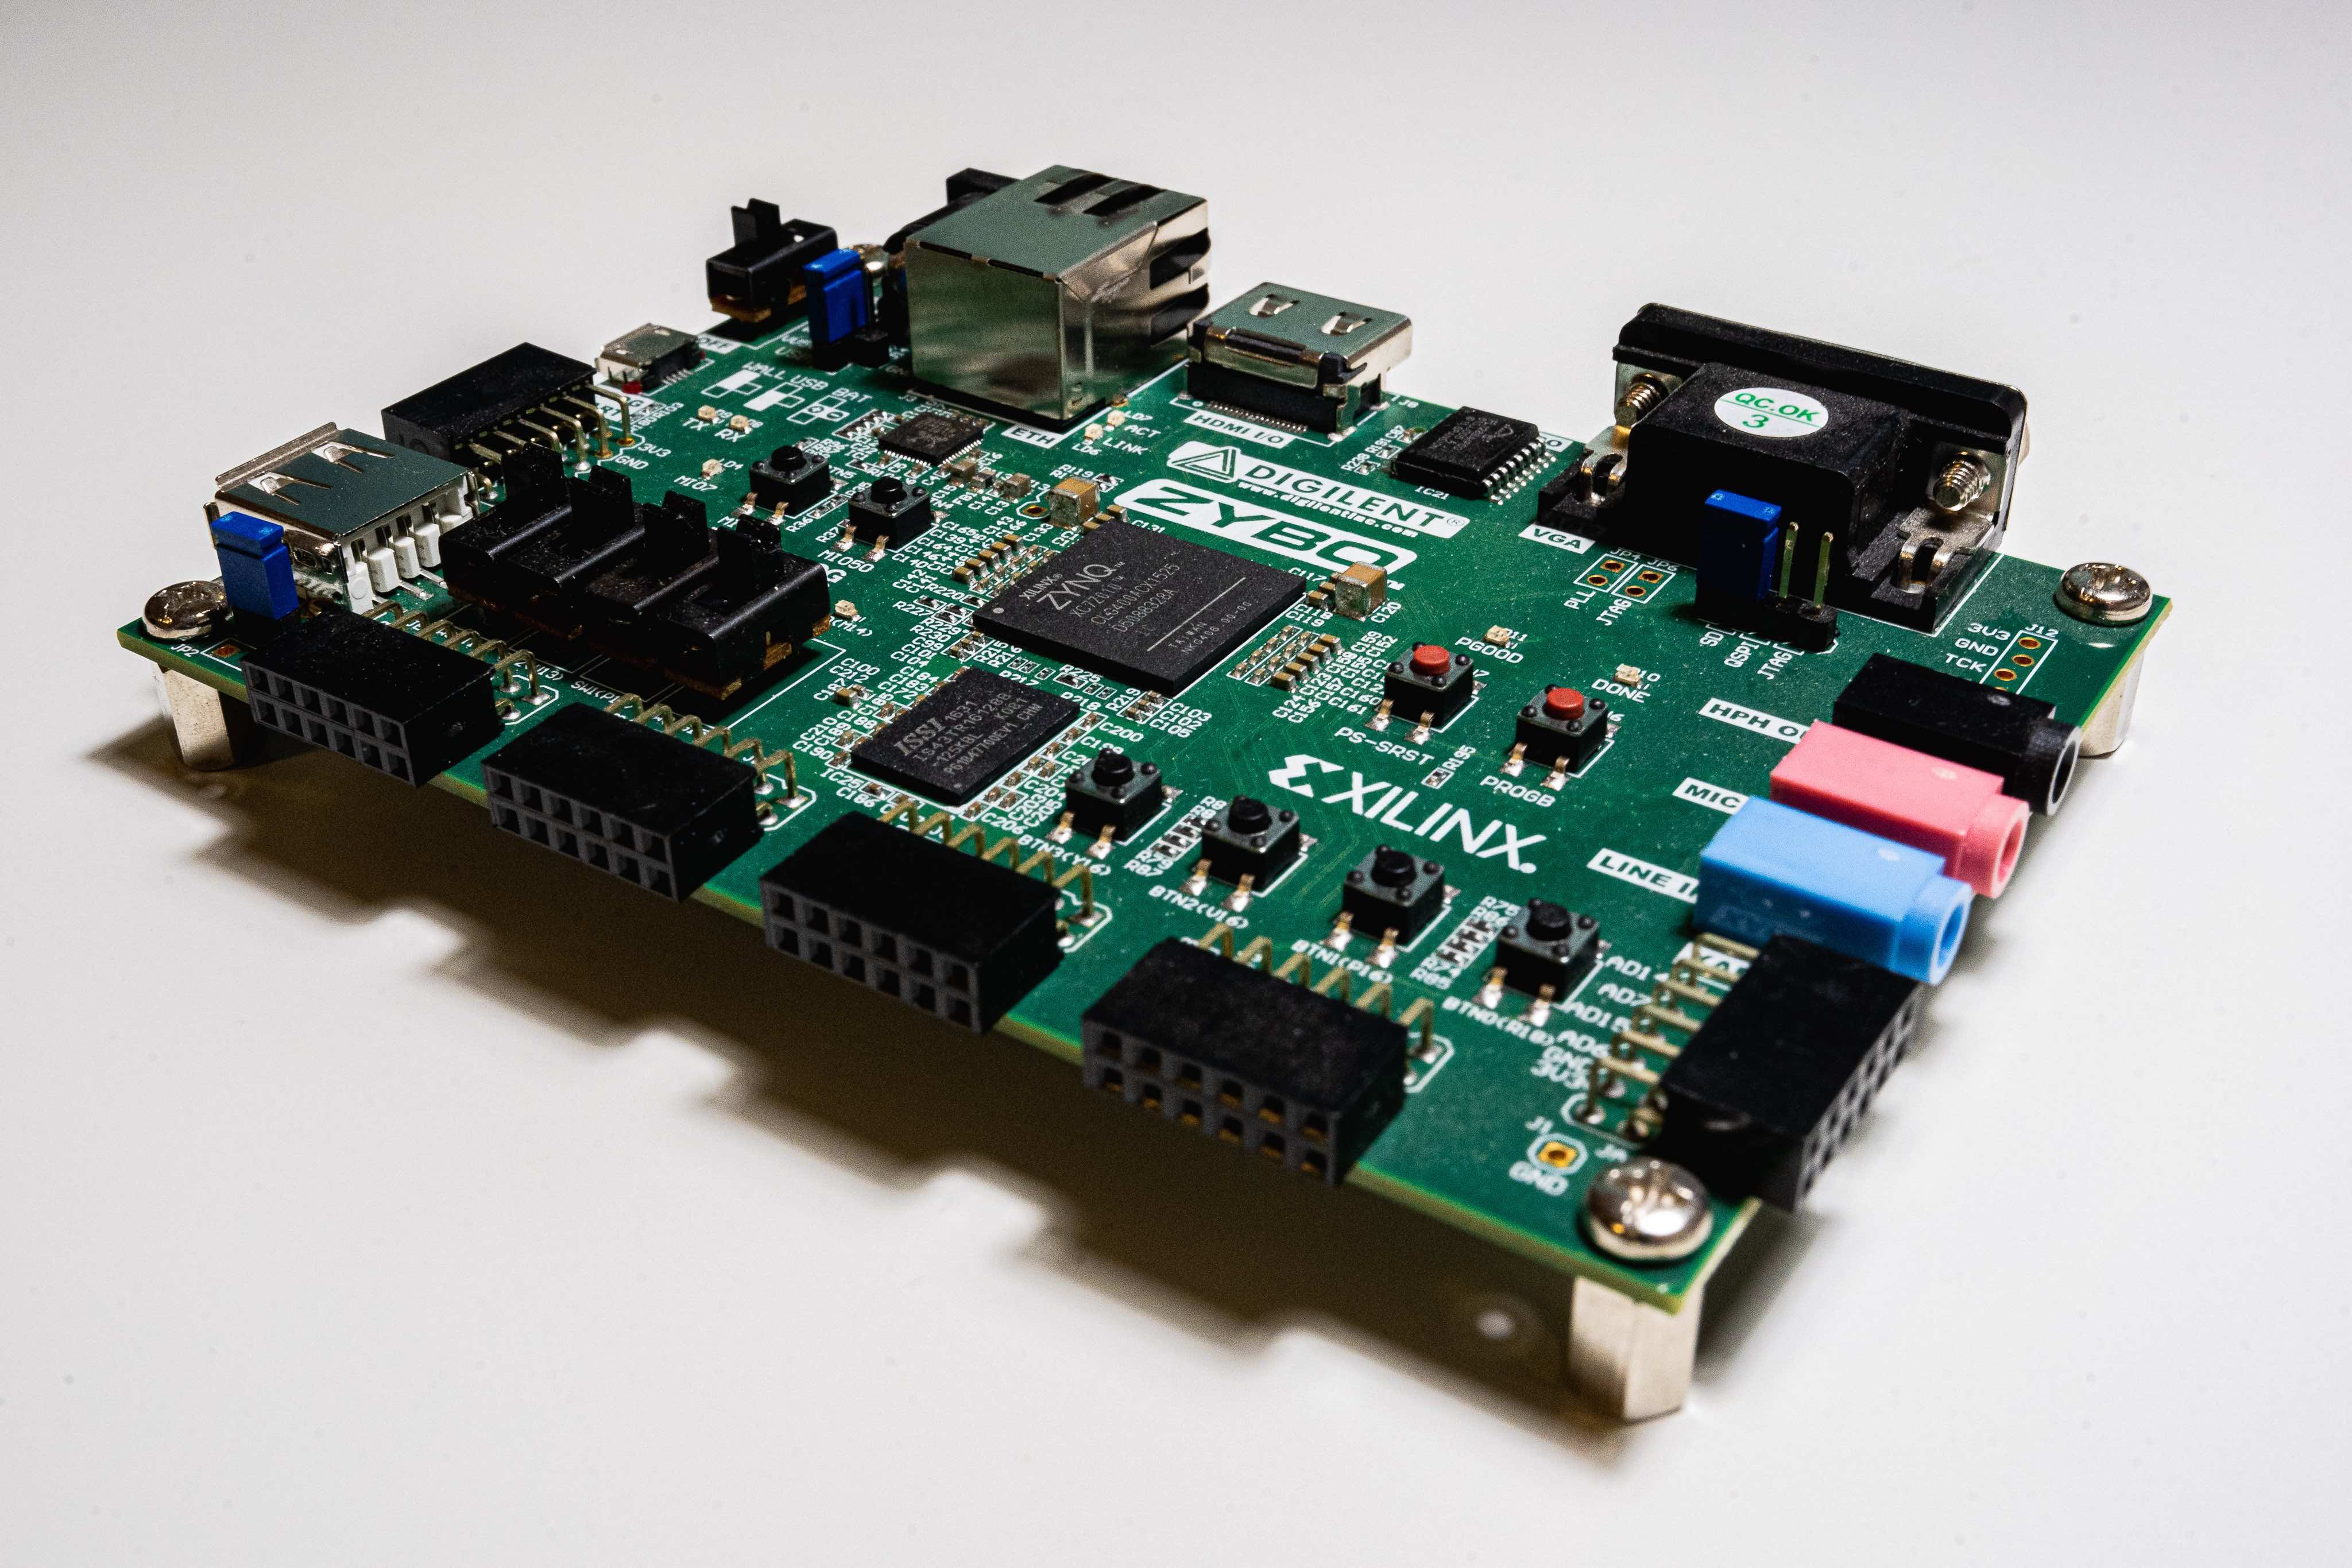
\includegraphics[width=0.85\textwidth]{src/jpg/digilent-zybo-foto-2.jpeg} 
					\caption{Vývojová deska Digilent ZYBO Zynq-7000 ARM/FPGA SoC Trainer Board – boční pohled.}
					\label{fig:digilent-zybo-foto-2}
			\end{figure}

		\subsection{Základní přehled}
		\subsubsection{CPU a FPGA čip}
			Hlavní částí vývojové desky je čip, obsahující FPGA a CPU jednotky zakomponované v~jedné polovodičové struktuře. Jak již bylo zmíněno v~části \hyperref[subsec:hardware-accelerated-applications]{\textit{Hardware Accelerated Applications}}, tato struktura se nazývá heterogenní.\par
			Deska obsahuje čip Xilinx Zynq-7000 (typ XC72010), který umožňuje pro vývoj aplikací použít SDK od firmy Xilinx. V~tomto čipu je integrován dvou jádrový procesor ARM Cortex-9, který slouží jako pro řízení akcelerovaných aplikací na Xilinx FPGA sedmé série. Detailní schéma blokové architektury SoC s~označním sběrnic a komunikace jednotlivých částí čipu je zobrazené na obr. \ref{fig:zynq-block-diagram-detailed}.\par
			Z~naznačené architektury je možné vyvodit, že se SoC skládá ze dvou hlavních částí, které je možné dále rozdělit na jednotlivé bloky:
			\begin{itemize}
				\item Processing System (PS),
				\begin{itemize}
					\item Application processor unit (APU),
					\item Memory interfaces,
					\item I/O peripherals (IOP),
					\item Interconnect,
				\end{itemize}
				\item Programmable Logic (PL).
			\end{itemize}
			\vspace*{0.25cm}
			\noindent\textbf{Blok PS}\\
			Blok PS se skládá z~dílčích bloků, které neslouží k~akceleraci aplikací, ale k~podpoře běhu hostitelského programu. Blok PS reprezentuje prakticky celou architekturu čipu vyjma části věnované PL.\par\vspace*{0.25cm}
			\noindent\textbf{Blok APU}\\
			Blok APU obsahuje CPU Cortex-A9 a další podpůrné bloky jako např. přímý přístup do paměti (DMA controller), Genral interrupt controller (GIC) pro maskování a ovládání přerušení, watchdog a další podpůrné bloky.\par\vspace*{0.25cm}
			\noindent\textbf{Blok Memory interfaces}\\
			Memory interfaces slouží k~přístupu APU a PL k~pamětím typu DDR3, DDR3L, DDR2 a LPDDR-2. Je možné také vybrat, zda šířka sběrnice bude 16, nebo 32 bitů. K~dispozici jsou zakoponované kotroléry přenosu dat pro optimalizaci rychlosti, Static Memory Controller nebo Quad-SPI Controller.\par\vspace*{0.25cm}
			\noindent\textbf{Blok IOP}\\
			IOP se skládá ze standardizovaných rozhraní vhodných pro průmyslovou komunikaci. Obsahuje nař. GPIO, Gigabit Ethernet, dva bloky USB Controller, dva bloky SD/SDIO Controller pro bootování SD karty, dva bloky SPI Controller, dva bloky CAN Controller, dva bloky UART Controller a dva bloky I2C Controller.\par\vspace*{0.25cm}
			\noindent\textbf{Blok Interconnect}\\
			Blok Interconnect, resp. na obr. \ref{fig:zynq-block-diagram-detailed} označený Central Interconnect slouží k~propojení jednotlivých bloků SoC dle požadované technologie a rychlosti.\par\vspace*{0.25cm}
			\noindent\textbf{Blok PL}\\
			Blok PL reprezentuje logické programovtelné pole (FPGA), v~němž jsou zakomponovány další podpůrné bloky jako např. blok zpracování digitálních signálů, řízení taktovacích hodin, analogově digitální převodník (ADC) apod.\par\vspace*{0.35cm}
			\noindent Detailní technické specifikace, složení a parametry jmenovaných bloků a jsou uvedeny v~\cite{xilinx-zynq-7000-technical-reference-manual}.
			% \begin{figure}[htbp!]
			% 	\centering
			% 		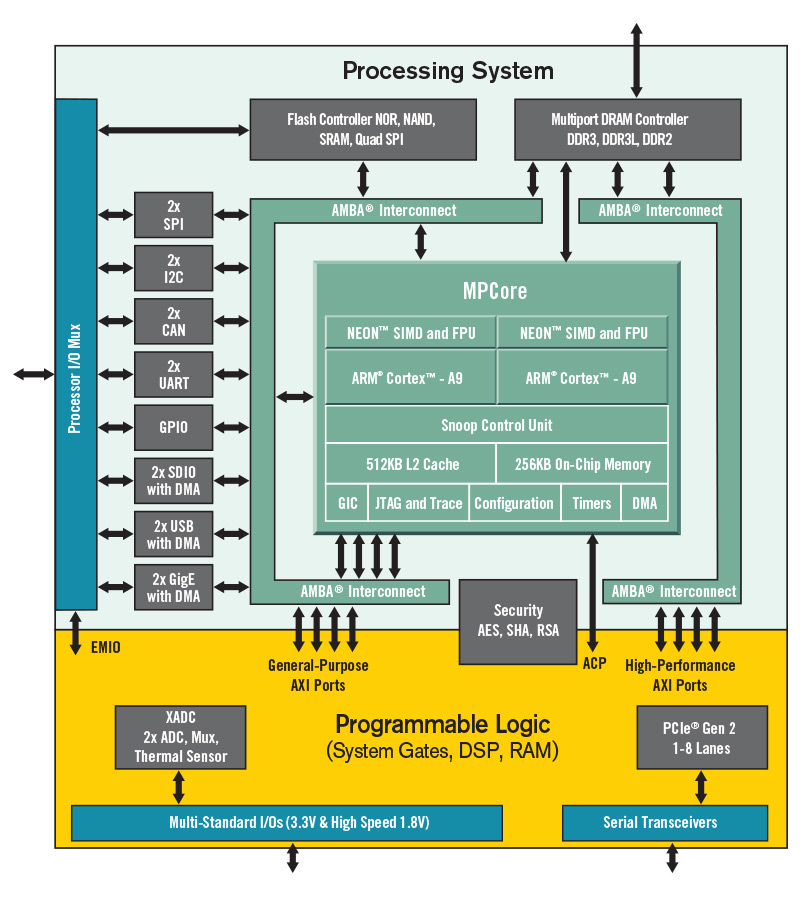
\includegraphics[width=0.75\textwidth]{src/png/zynq-mp-core-dual.png} 
			% 		\caption{Blokové schéma čipu Zynq-7000, umístěného na vývojové desce \textit{Digilent ZYBO Zynq-7000 ARM/FPGA SoC Trainer Board}. (převzato z \cite{xilinx-zynq-7000-socs-with-hardware-and-software-programmability})}
			% 		\label{fig:zynq-mp-core-dual}
			% \end{figure}

			\begin{figure}[htbp!]
				\centering
					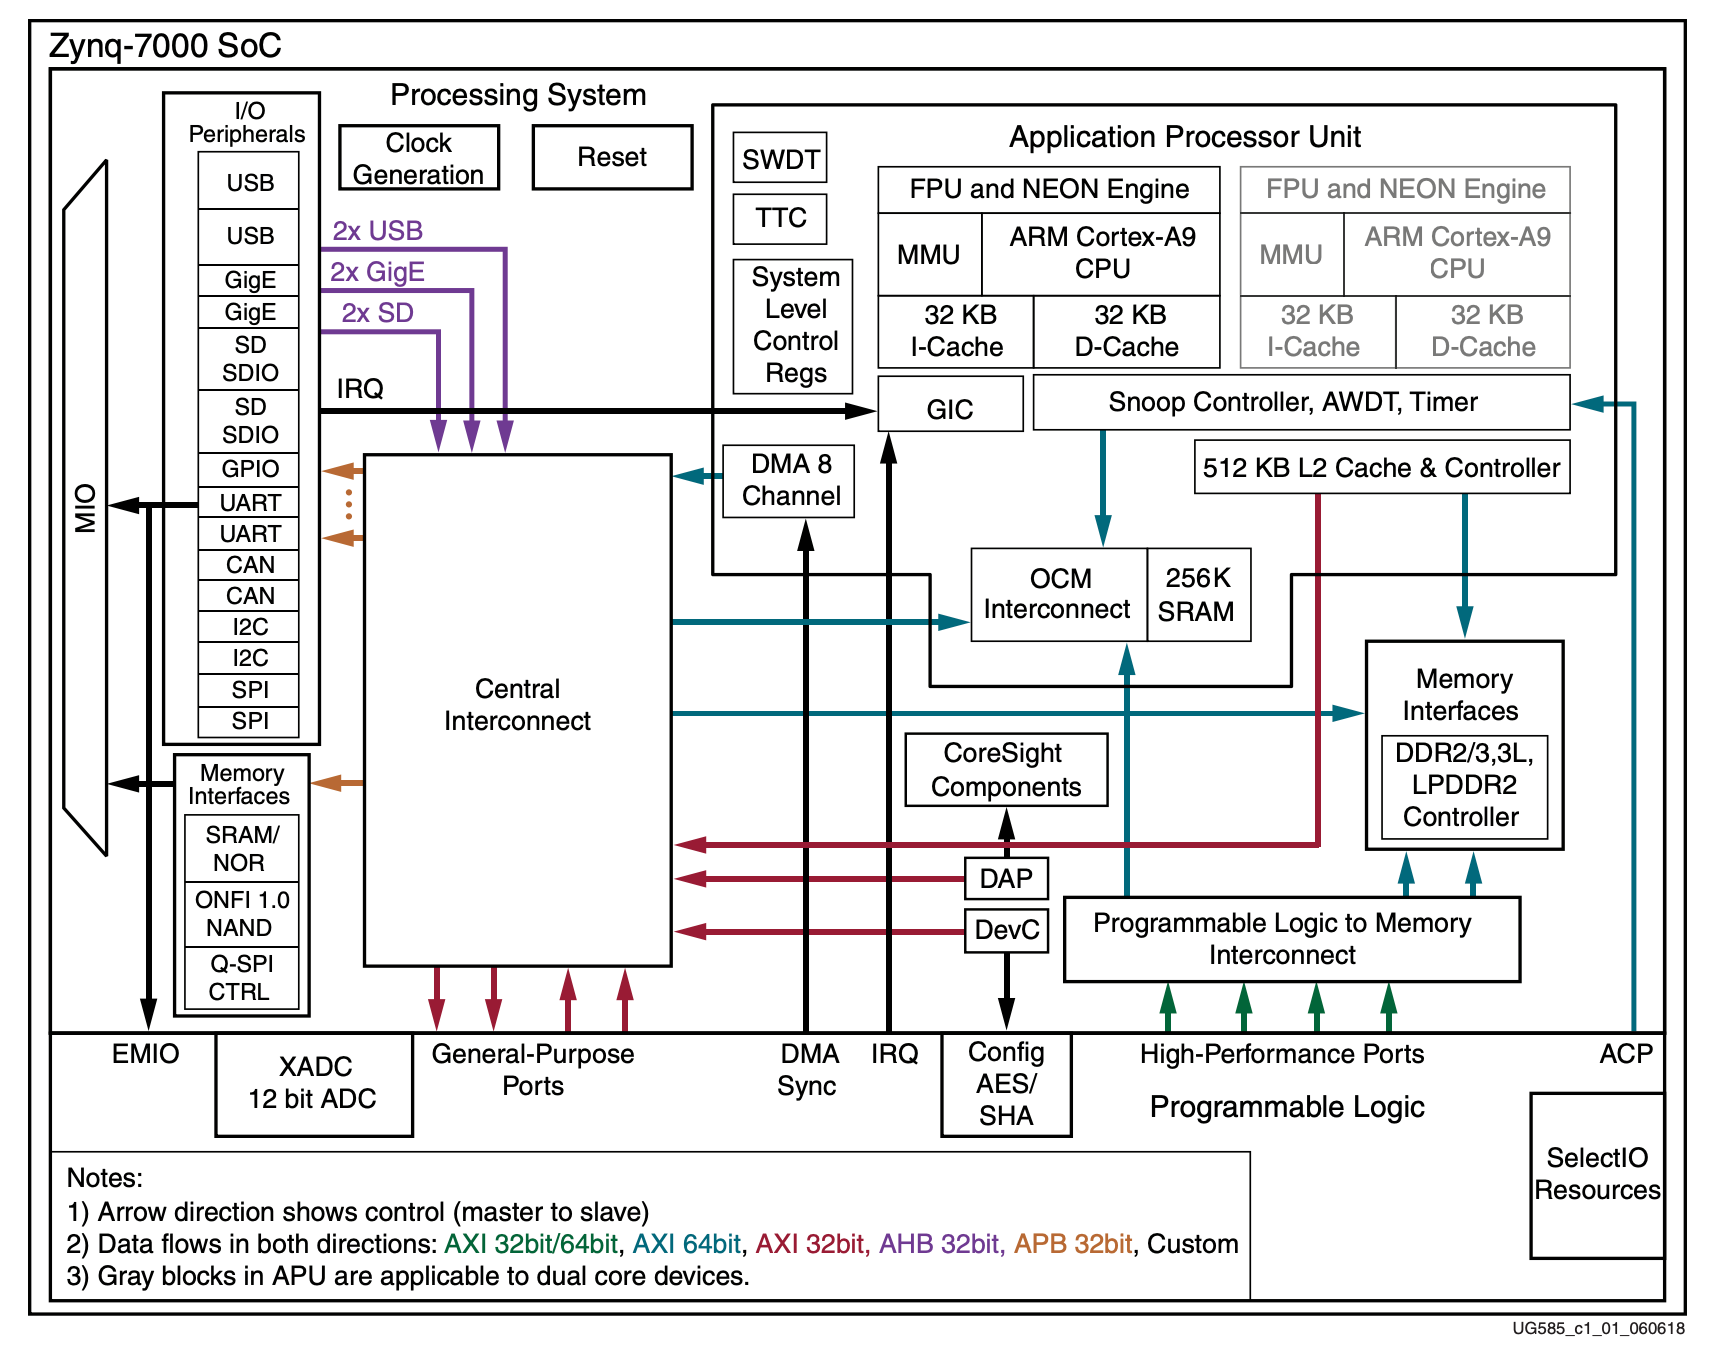
\includegraphics[width=0.90\textwidth]{src/png/zynq-block-diagram-detailed.png} 
					\caption{Detailní schéma čipu Zynq-7000, umístěného na vývojové desce \textit{Digilent ZYBO Zynq-7000 ARM/FPGA SoC Trainer Board}. (převzato z~\cite{xilinx-zynq-7000-technical-reference-manual})}
					\label{fig:zynq-block-diagram-detailed}
			\end{figure}
			\fbar
			\subsubsection{Uspořádání vývojové desky Zybo Zynq-7000}
				Na obr. \ref{fig:digilent-zybo-foto-1-oznacene} je zobrazen horní pohled na vývojovou desku, na které jsou vyznačeny významné části, kterým je vhodné věnovat pozornost. Číselné označení koresponduje s~označením a vysvětlivkou v~tabulce \ref{tab:digilent-zybo-zynq-7000-description}. Pro úplnost je spodní strana desky zobrazena na obr. \ref{fig:digilent-zybo-foto-3}.

				\begin{figure}[H]
					\centering
						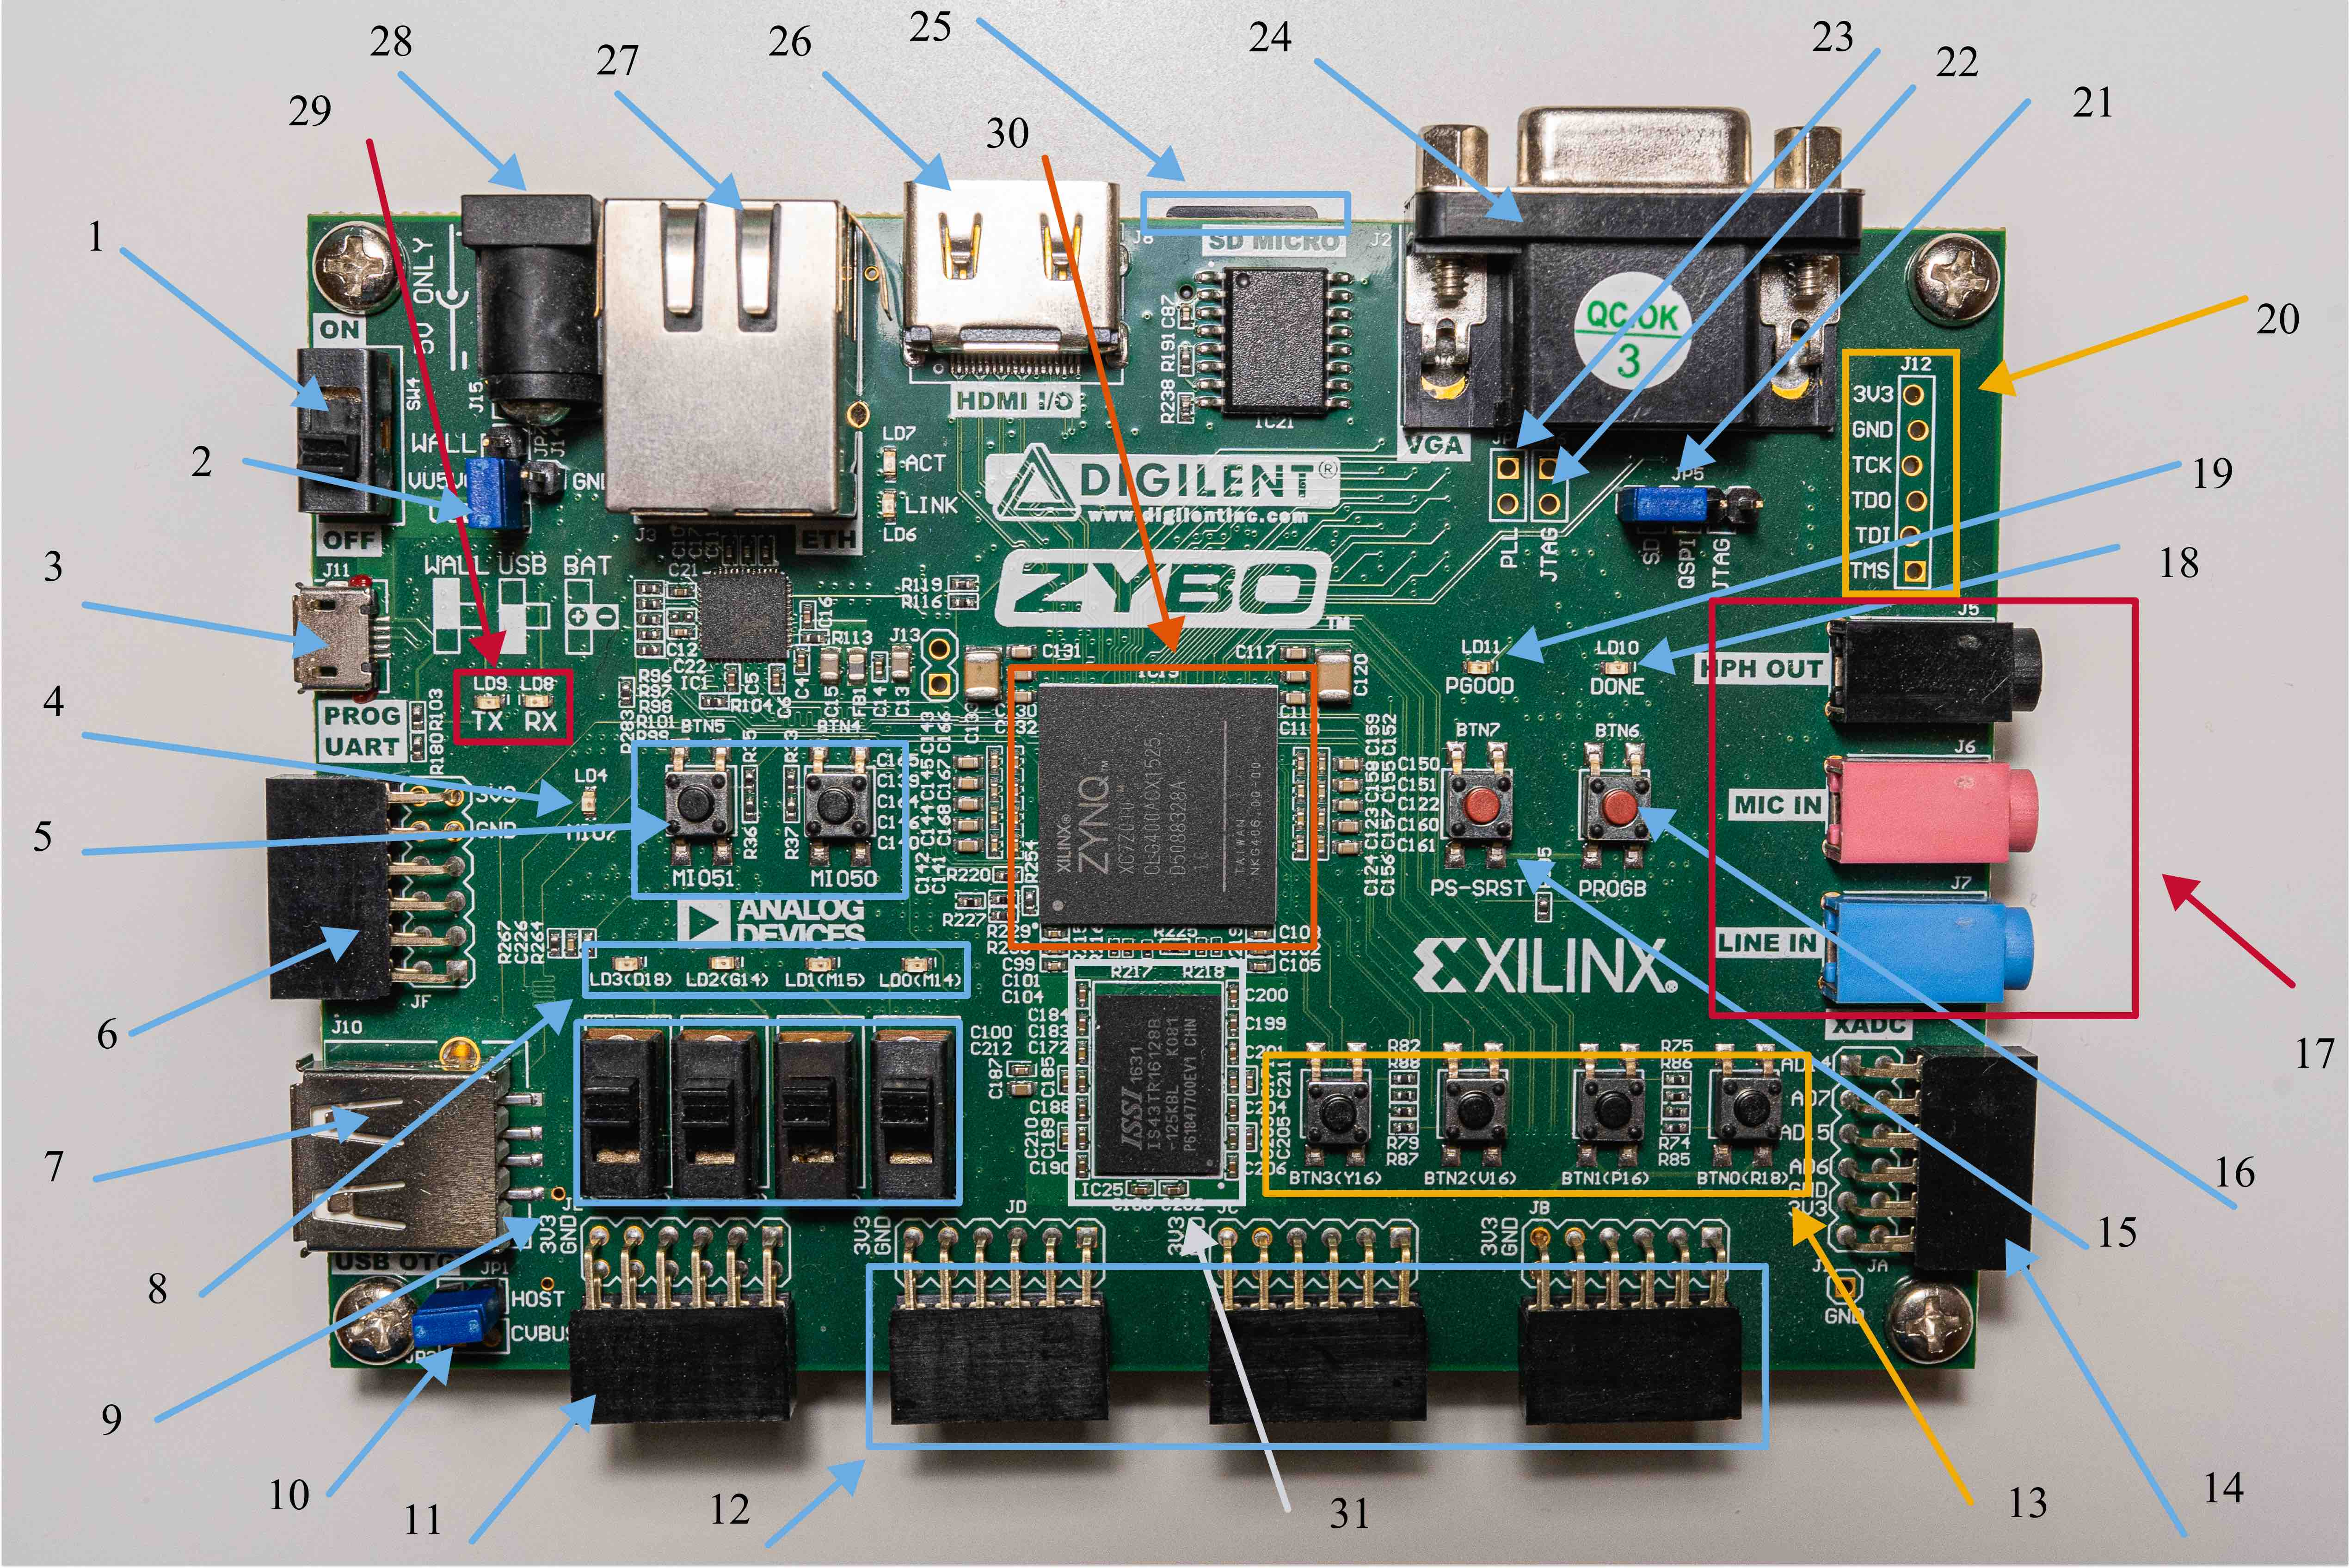
\includegraphics[width=1\textwidth]{src/jpg/digilent-zybo-foto-1-oznacene.jpeg} 
						\caption{Vývojová deska Digilent ZYBO Zynq-7000 ARM/FPGA SoC Trainer Board vrchní pohled s~vyznačením komponent.}
						\label{fig:digilent-zybo-foto-1-oznacene}
				\end{figure}

				\begin{figure}[H]
					\centering
						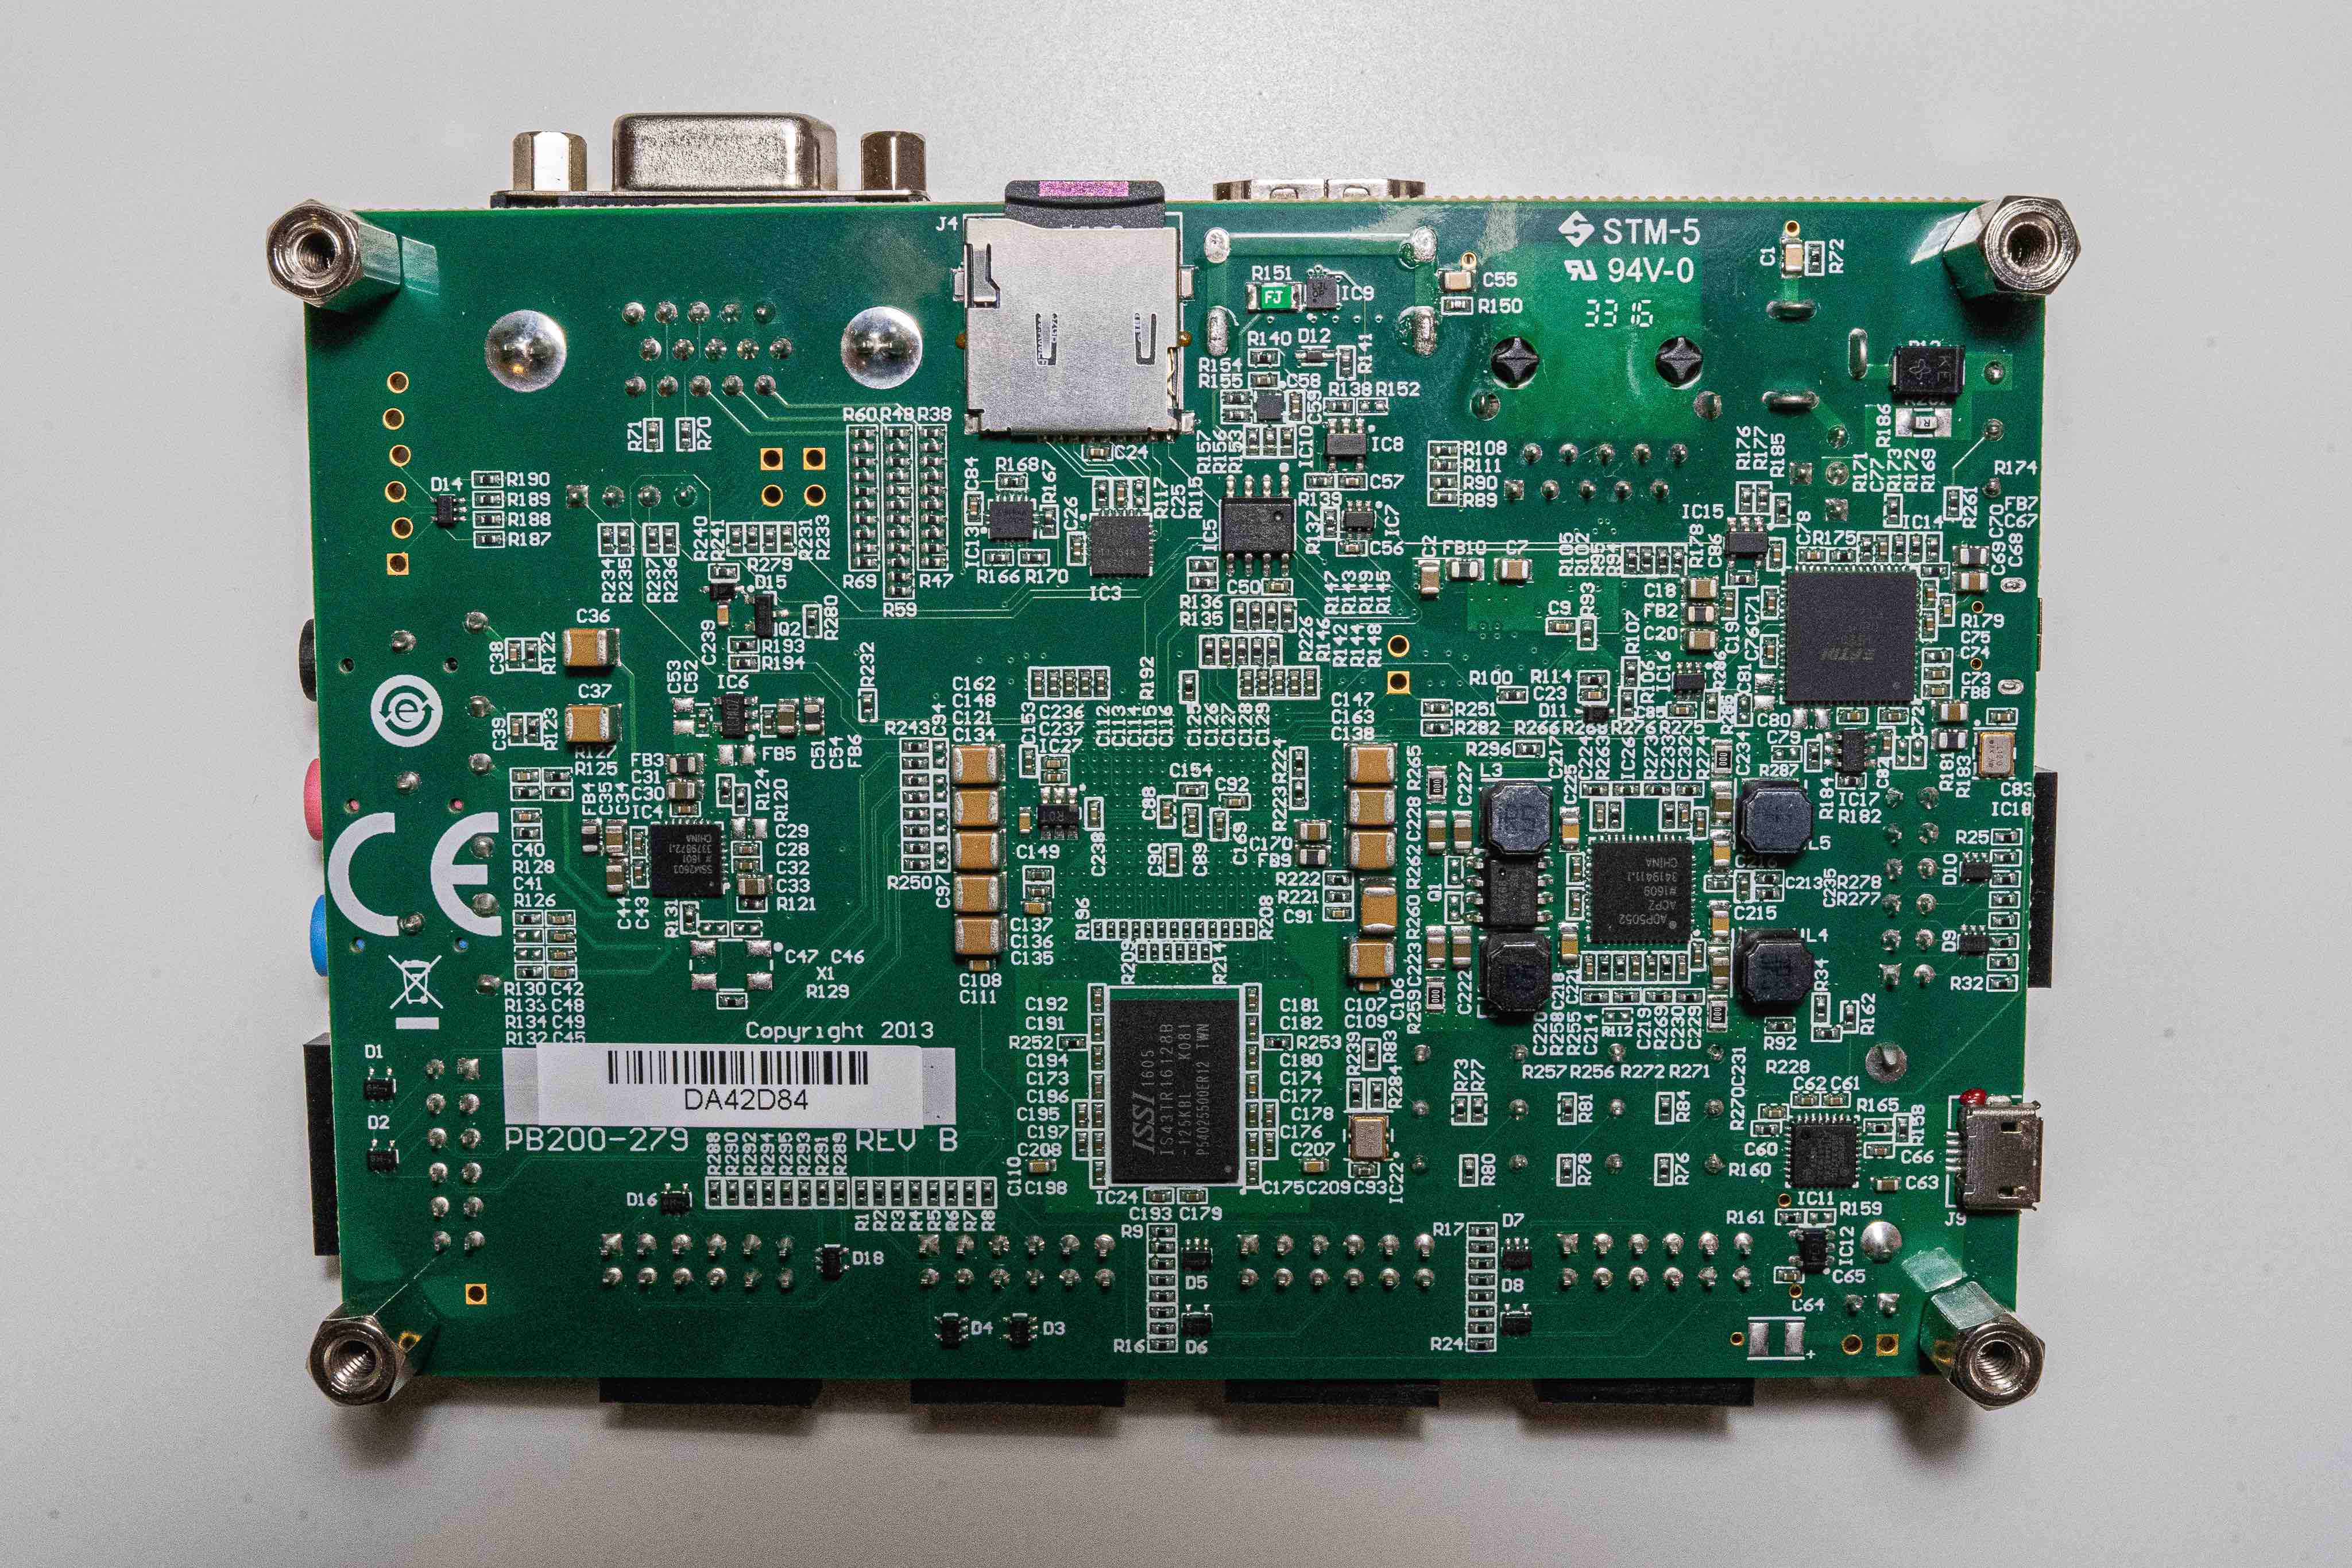
\includegraphics[width=1\textwidth]{src/jpg/digilent-zybo-foto-3.jpeg} 
						\caption{Vývojová deska Digilent ZYBO Zynq-7000 ARM/FPGA SoC Trainer Board – spodní pohled.}
						\label{fig:digilent-zybo-foto-3}
				\end{figure}

			\fbar
			\begin{table}[htbp!]
				\centering
				\caption{Popis označených komponent na vývojové desce Digilent Zybo Zynq-7000. (informace a značení převzaty z~\cite{digilent-zybo-reference-manual})}
			  \vspace*{0.15cm}
			   \resizebox{\textwidth}{!}
				{
				\begin{tabular}{!{\vrule width 2pt} c | l | l !{\vrule width 2pt}}\noalign{\hrule height 2pt}
				označení & popis &	poznámka \\
				\noalign{\hrule height 2pt}
				1 & Power Switch & galvanické sepnutí napájecího obvodu \\ \hline
				2 & Power Select Jumper and Battery Header & výběr napájecího vstupu konektor, USB, baterie\\ \hline
				3 & Shared UART/JTAG USB port & komunikace UART a JTAG debugging\\ \hline
				4 & MIO LED & multiplexed LED – možnost výběru signálu\\ \hline
				5 & MIO Pushbuttons (2) & multiplexed input\\ \hline
				6 & MIO Pmod & možnost připojení periférií\\ \hline
				7 & USB OTG Connectors & USB port typ A/micro USB (spodní část)\\ \hline
				8 & Logic LEDs (4) & zobrazování 1/0\\ \hline
				9 & Logic Slide Switches (4) & logický vstup 1/0\\ \hline
				10 & USB OTG Host/Device Select Jumpers & výběr módu zařízení\\ \hline
				11 & Standard Pmod & chráněné Pmod, limitace max. přenosu informace\\ \hline
				12 & High-speed Pmods (3) & jako standard ale bez ochrany, vyšší rychlost\\ \hline
				13 & Logic Pushbuttons (4) & logický vstup 1/0\\ \hline
				14 & XADC Pmod & možnost  analog/digi input/output, spojeno s~ADC v~Zynq\\ \hline
				15 & Processor Reset Pushbutton & reset PL, paměti v~PS\\ \hline
				16 & Logic Configuration reset Pushbutton & reset PL, zrušení DONE informace\\ \hline
				17 & Audio Codec Connectors & stereo line in, mono mikrofon, stereo output\\ \hline
				18 & Logic Configuration Done LED & signál o~úspěšném dokončení konfigurace PL\\ \hline
				19 & Board Power Good LED & 1/0, 1 – nominální napětí na všech sběrnicích\\ \hline
				20 & JTAG Port for optional external cable & externí JTAG\\ \hline
				21 & Programming Mode Jumper & výběr „programovacího vstupu“, SD karta, QSPI, JTAG\\ \hline
				22 & Independent JTAG Mode Enable Jumper & JTAG mimo PS, viditelné pouze PL\\ \hline
				23 & PLL Bypass Jumper & přemostění PLL (CLK), pro možnost konfigurace PLL\\ \hline
				24 & VGA connector & připojení displaye\\ \hline
				25 & microSD connector & na spodní straně\\ \hline
				26 & HDMI Sink/Source Connector & input/ouput, nutné implementovat encoding a decoding v~logice\\ \hline
				27 & Ethernet RJ45 Connector & komunikace\\ \hline
				28 & Power Jack & napájení 5 V/2,5 A\\ \hline
				29 & TX/RX LED & indikace UART komunikace\\ \hline
				30 & Xilinx Zynq SoC & srdce desky\\ \hline
				31 & DDR2 Memory & RAM\\\noalign{\hrule height 2pt}
				\end{tabular}
				}
				\label{tab:digilent-zybo-zynq-7000-description}
			\end{table}


			

		\fbar
		\section{Vývojová deska Xilinx Kria KR260}
				Deska od firmy Digilent, představená v~\hyperref[sec:vyvojova-deska-digilent-zybo]{\textit{Vývojová deska Digilent Zybo}}, je vhodná pouze pro prvotní seznámení s~vytvářením akcelerovaných aplikací. Pro náročnější aplikace, které při potřebují při využití většího množství LUTs nebylo v~této práci možné Zybo použít. Vývojová deska Kria KR260 disponuje dostatečným množstvím LUTs a díky svým moderním komponentám a prvkům, může efektivně sloužit k~vytváření náročnějších aplikací.\par
				Hlavní částí vývojové desky KR260 je „modul“ \textit{Kria K26 System-on-Module}. Tudíž oproti Digilent Zybo, které využívá SoC, deska KR260 využívá SoM. Přednosti jednotlivých architektur byly již představeny v~části \hyperref[sec:system-on-a-chip]{\textit{System on a chip}} a \hyperref[sec:system-on-modules]{\textit{System on modules}}. Po ukončení vývoje aplikace na vývojové desce (a také po ukončení vytvářeného návrhu CC) je možné zakoupit pro aplikaci v~průmyslu samotný modul ve vhodné variantě. V~této práci je ovšem využíván standardní vývojový „Starter kit“ s~deskou KR260, jejíž komponenty je vhodné představit.

				\begin{figure}[H]
					\centering
						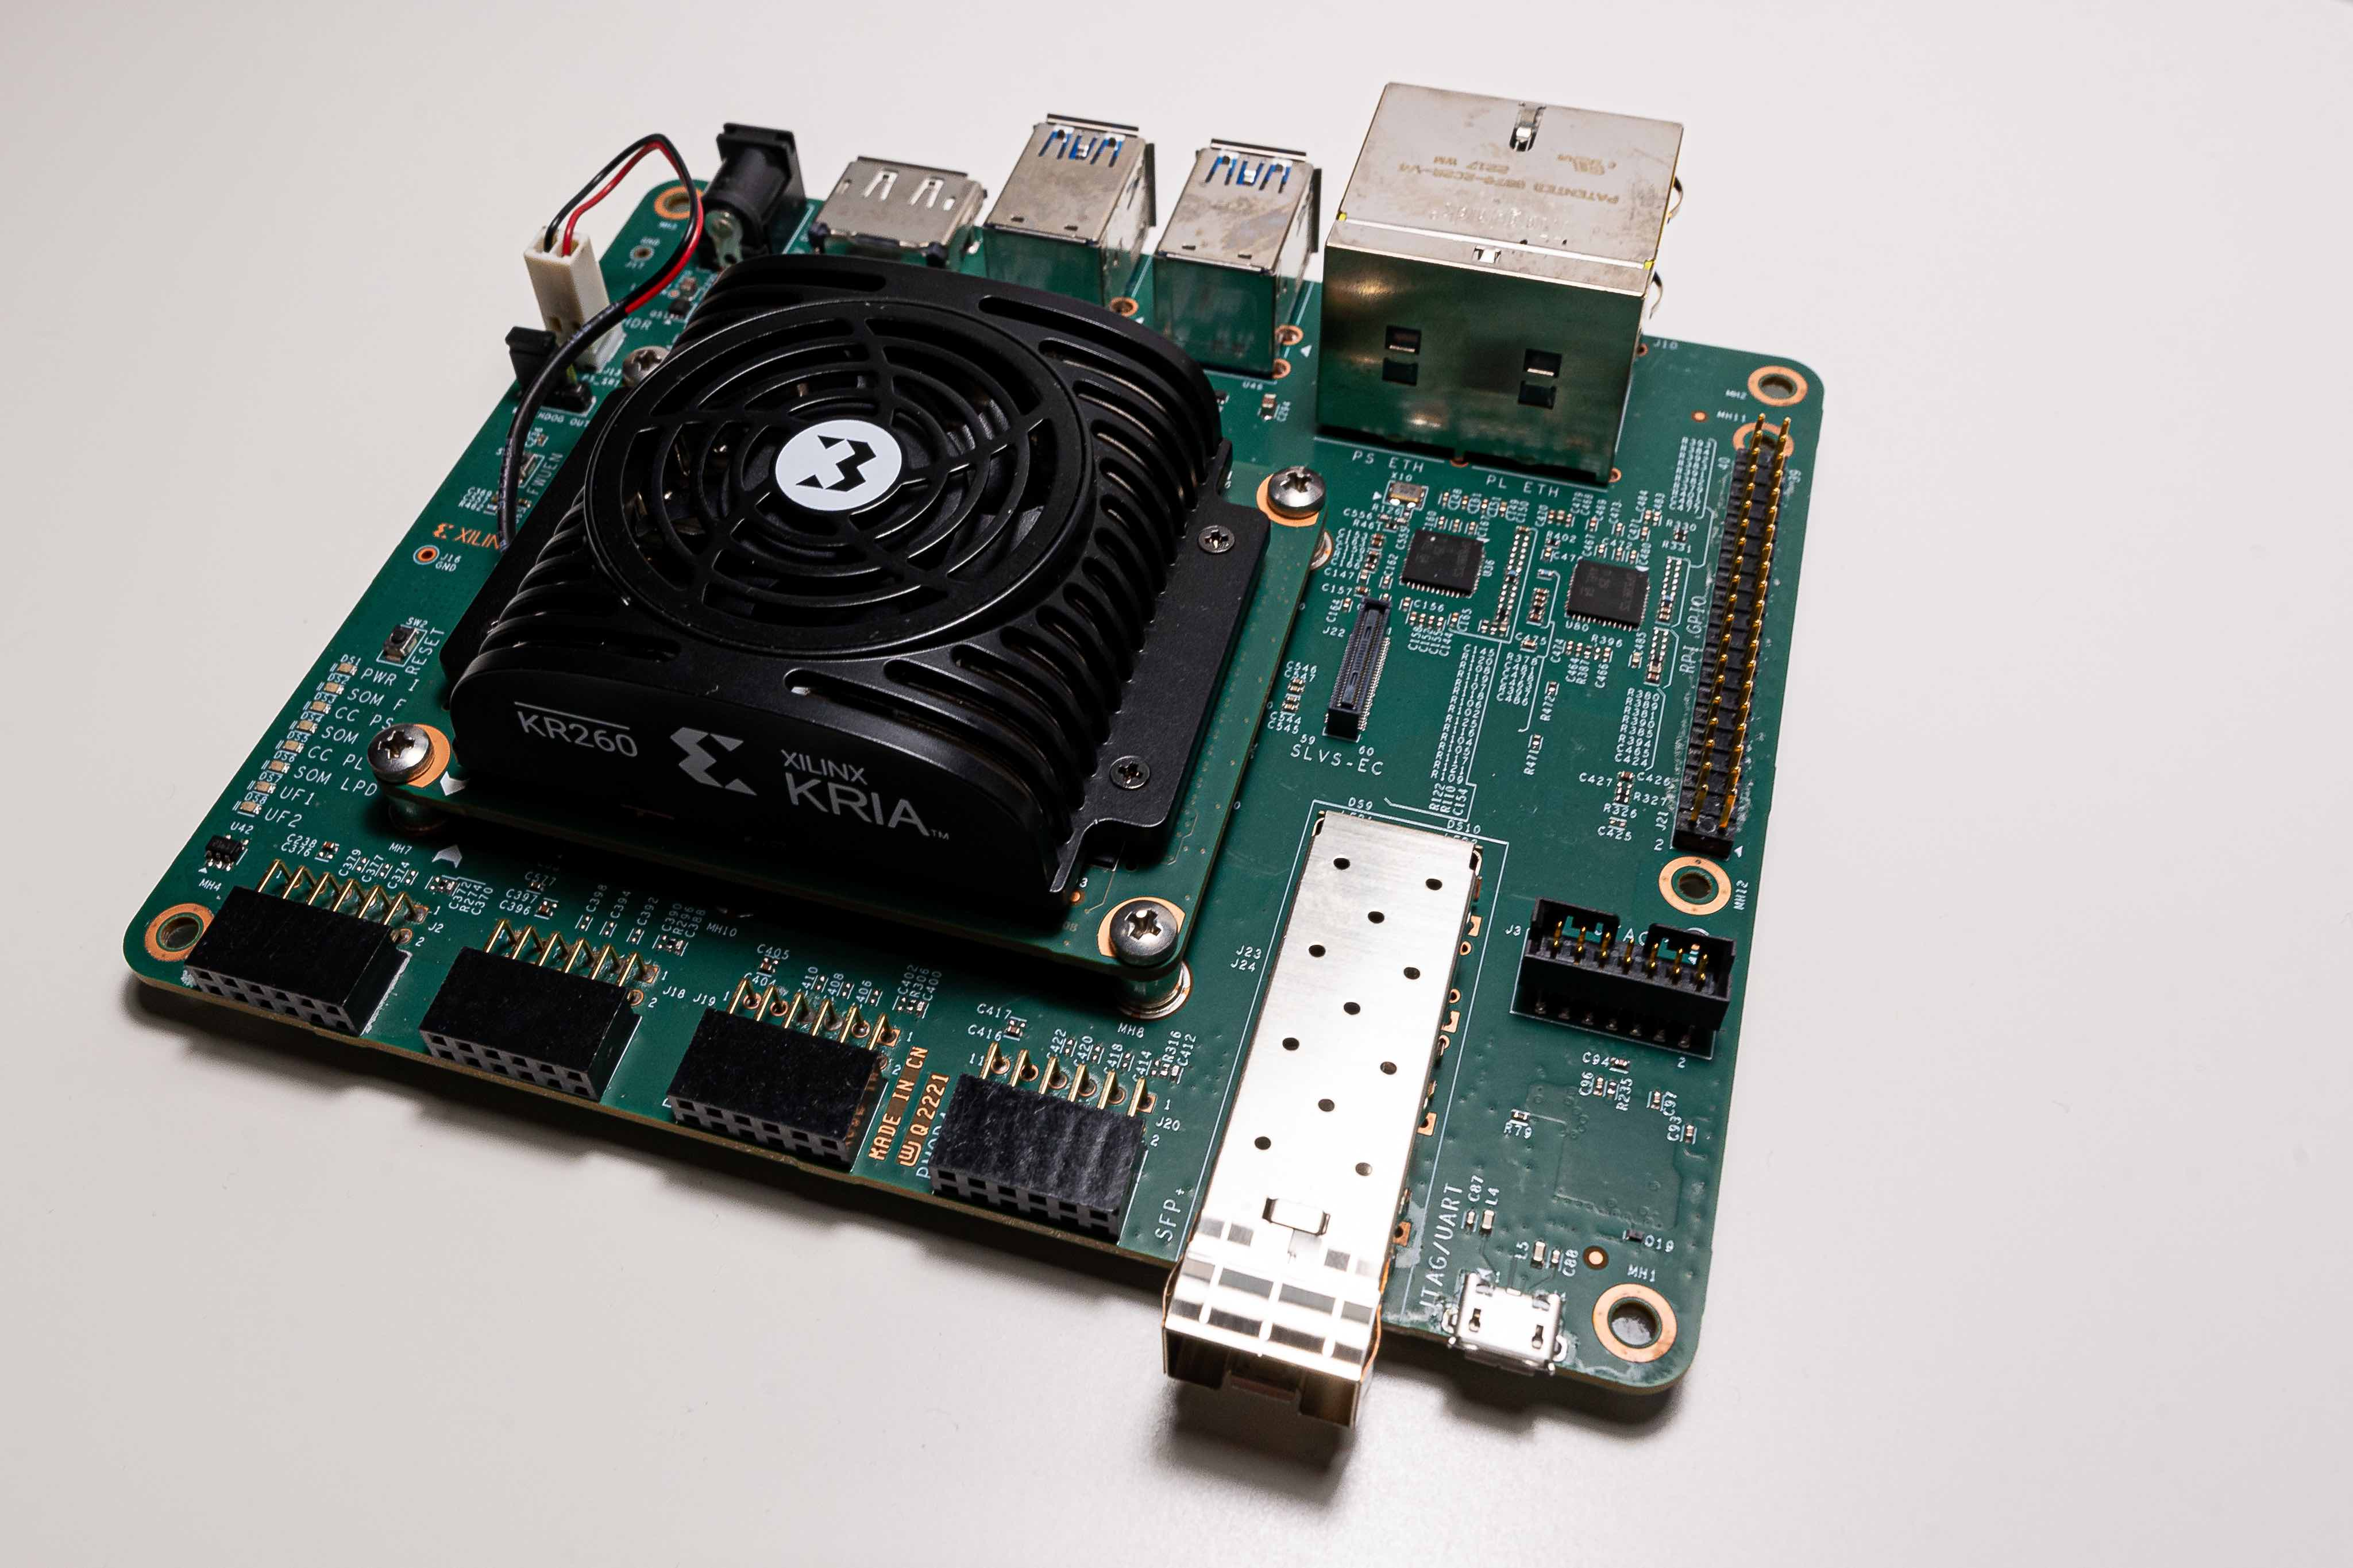
\includegraphics[width=1\textwidth]{src/jpg/xilinx-kria-foto-1.jpeg} 
						\caption{Vývojová deska Xilinx Kria KR260 – boční pohled.}
						\label{fig:xilinx-kria-foto-1}
				\end{figure}

				\subsection{Základní přehled}
					\subsubsection{CPU a FPGA čip}
						Strukturu SOM je možné popsat jako modernější a rozmanitější vylepšení SoC. Opět se vve struktuře nachází hlavní základní bloky pro PS a PL. Ukázkový blokový diagram struktury udávané výrobcem je na obr. \ref{fig:xilinx-kria-k26-block-diagram}.

						\begin{figure}[htbp!]
							\centering
								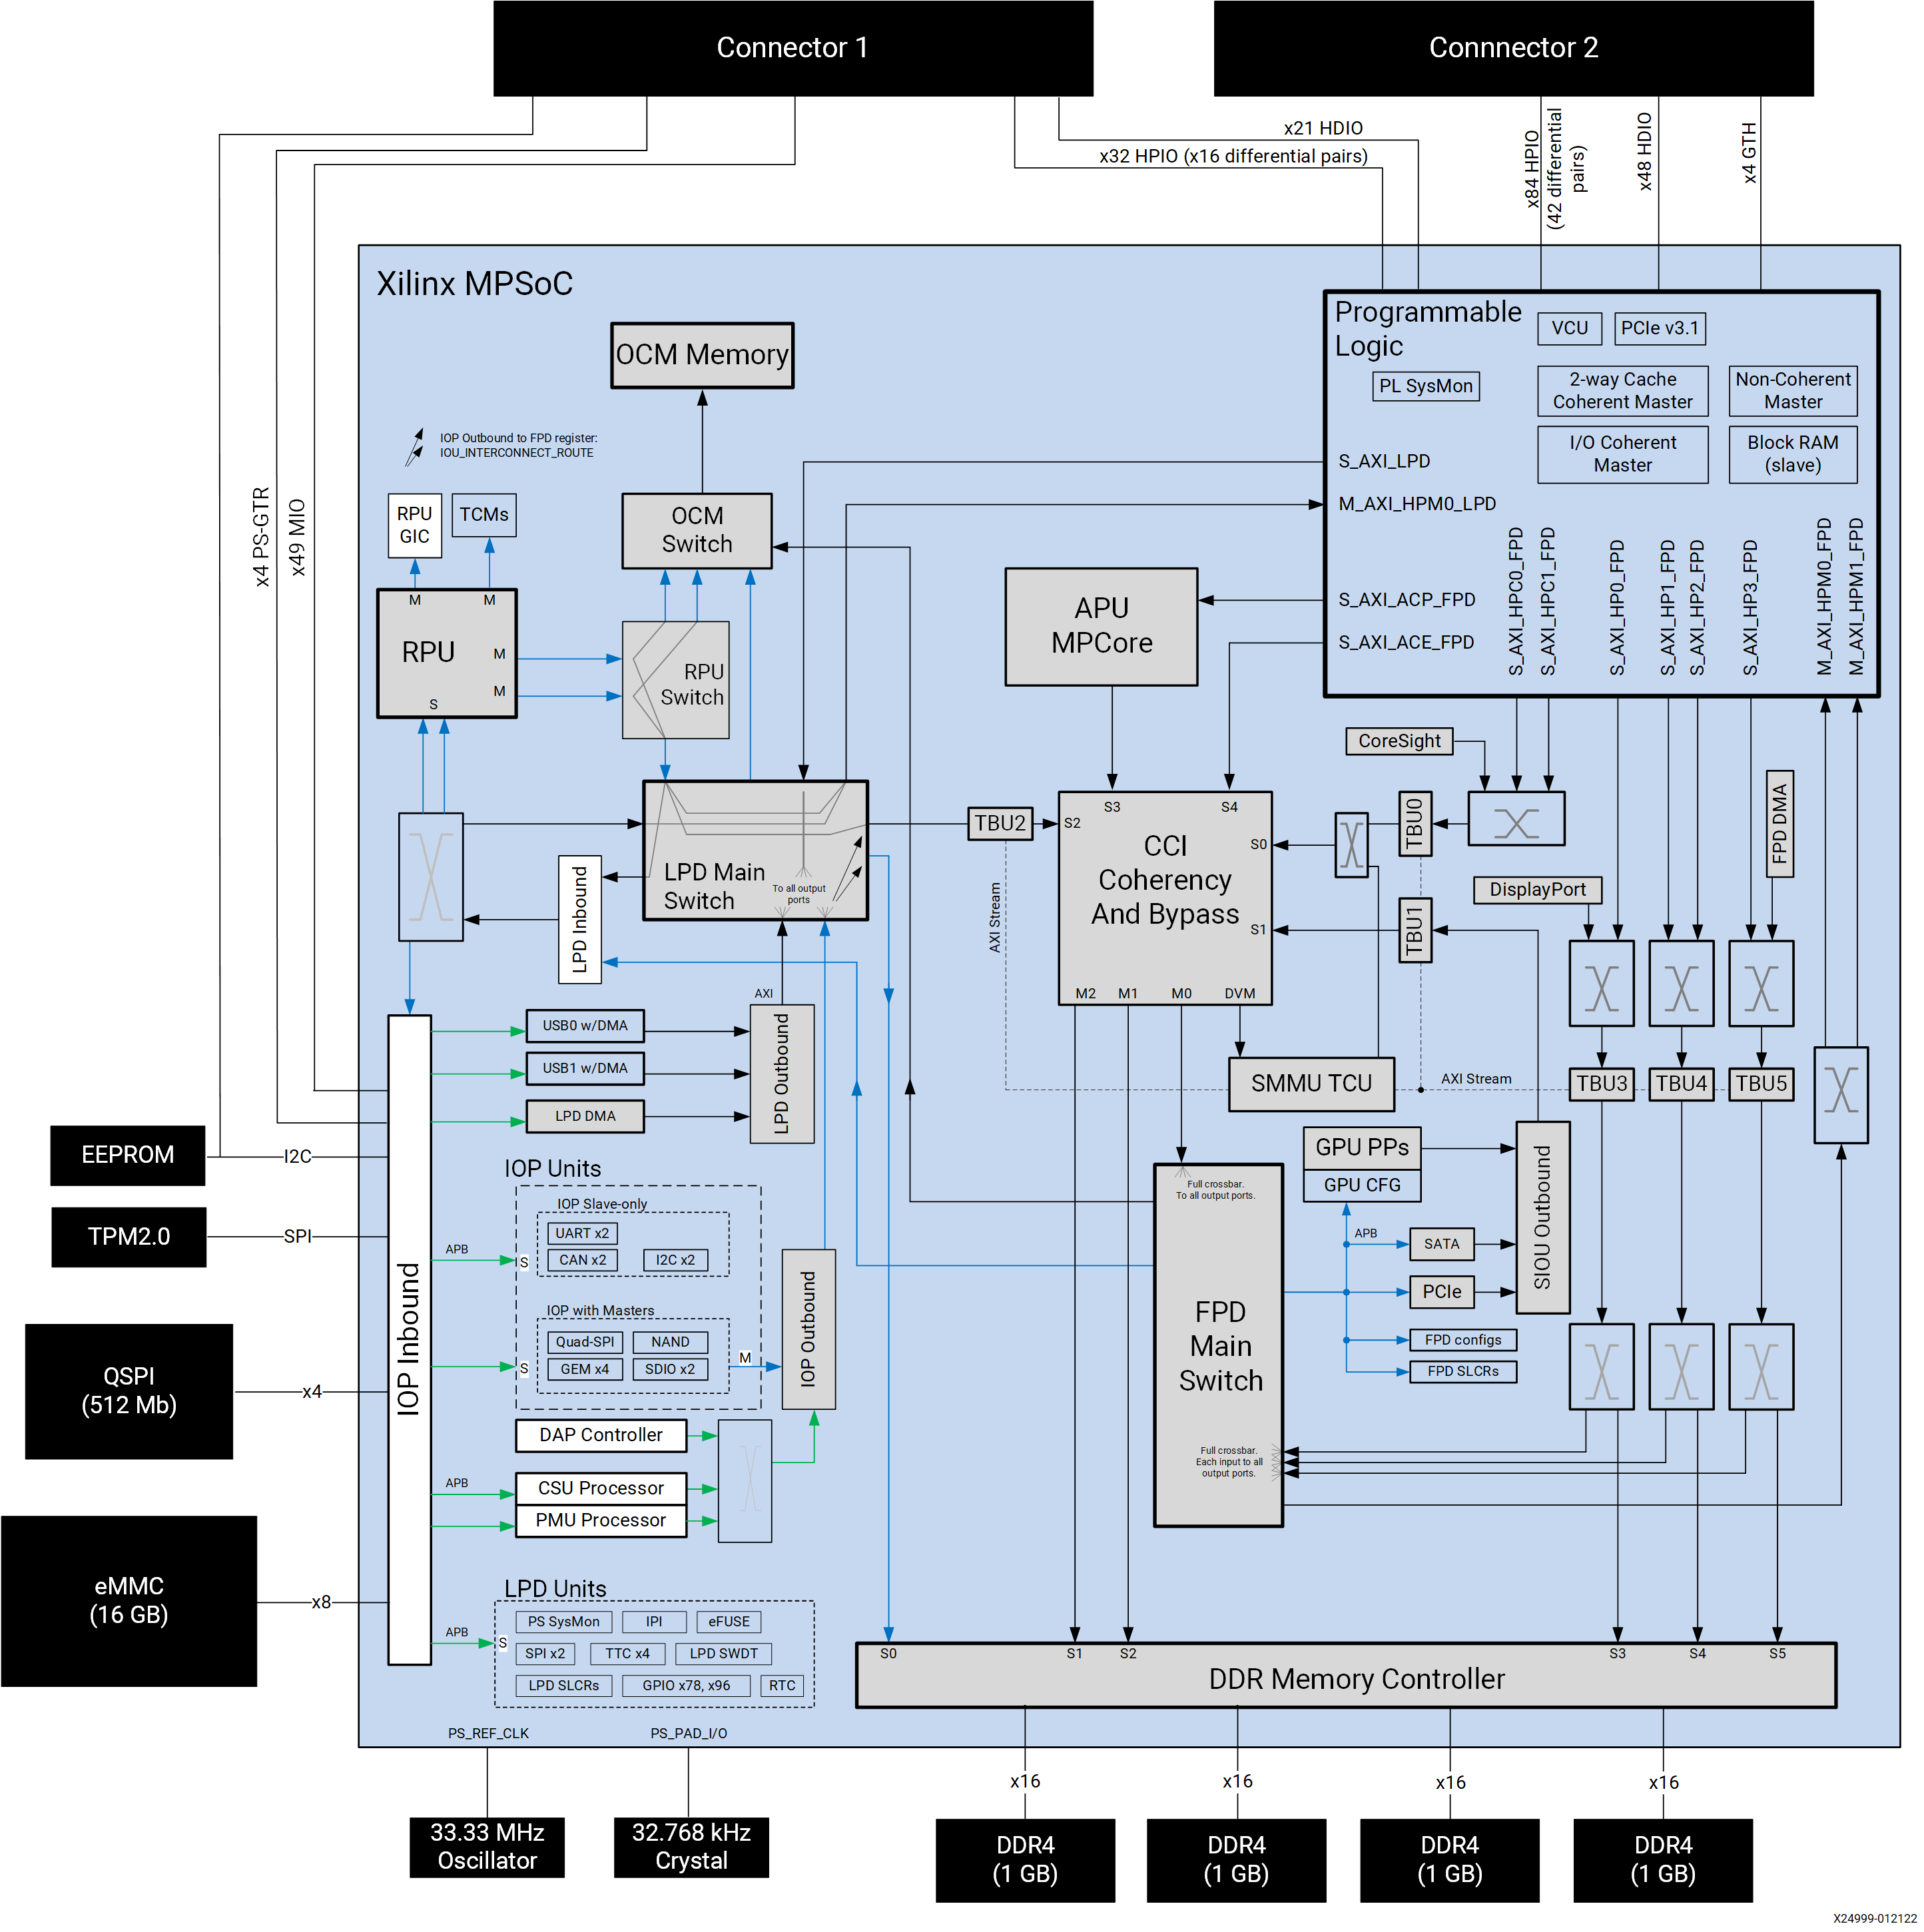
\includegraphics[width=1\textwidth]{src/jpg/xilinx-kria-k26-block-diagram.jpg} 
								\caption{Blokový diagram K26 SOM Kria. \cite{kria-k26-som-ds}}
								\label{fig:xilinx-kria-k26-block-diagram}
						\end{figure}
						\fbar

						Největšími rozdíly mezi použitými deskami Zybo a Kria je např. velikost operační paměti, počet jader a taktovací frekvence procesorů v~PS, počet LUTs nebo logických buněk v~FPGA (PL). Úplné specifikace pro K26 SOM je možné nalézt v~\cite{kria-k26-som-ds}.

				\subsection{Uspořádání vývojové desky}
				Na obr. \ref{fig:xilinx-kria-foto-2-oznacene} je zobrazen horní pohled na vývojovou desku, na které jsou vyznačeny významné části, kterým je vhodné věnovat pozornost. Číselné označení koresponduje s~označením a vysvětlivkou v~tabulce \ref{tab:xilinx-kria-description}. Na spodní straně desky je umístěn slot pro SD kartu, na kterou je umisťován operační systém pro PS. Pro úplnost je spodní strana desky zobrazena na obr. \ref{fig:xilinx-kria-foto-3}.
				\fbar
				\begin{table}[htbp!]
					\centering
					\caption{Popis označených komponent na vývojové desce  Xilinx Kria KR260. (informace a značení převzaty z~\cite{kria-kr260-robotics-starter-kit-user-guide})}
			  		\vspace*{0.15cm}
			   		\resizebox{\textwidth}{!}
						{
							\begin{tabular}{!{\vrule width 2pt} c | l | l !{\vrule width 2pt}}\noalign{\hrule height 2pt}
							označení & popis &	poznámka \\
							\noalign{\hrule height 2pt}
							1 & SOM modul na BB a Fansink & -  \\ \hline
							2 & J13 Fan Power & napájení větráku chladiče  \\ \hline
							3 & J1 watchdog & -  \\ \hline
							4 & SW1 Firmware Update & -  \\ \hline
							5 & SW2 Reset & -  \\ \hline
							6 & DS1–DS6 Power Status LEDs & pokud vše ok, jsou zbarveny zeleně  \\ \hline
							7 & DS7–DS8 (UF1 a UF2) Uživatelsky ovládané LED & -  \\ \hline
							8 & J2, J18, J19, J20 Pmod konektory & -  \\ \hline
							9 & J23 a J24 SFP+ & optický konektor  \\ \hline
							10 & J4 Micro USB & UART/JTAG  \\ \hline
							11 & J3 PC4 JTAG & -  \\ \hline
							12 & J22 SLVS-EC & konektor pro připojení kamery  \\ \hline
							13 & DS36 Raspberry Pi HAT & -  \\ \hline
							14 & J10A, J10B RJ-45 PL Ethernet & konektor připojen přes PL  \\ \hline
							15 & J10C, J10D RJ-45 PS Ethernet & konektor připojen do PS  \\ \hline
							16 & U46 USB3.0 & -  \\ \hline
							17 & U44 USB3.0 & -  \\ \hline
							18 & DS36 PS Status LED & -  \\ \hline
							19 & DS35 HeartBeat LED & -  \\ \hline
							20 & DS34 PS Done LED & -  \\ \hline
							21 & J6 DisplayPort & -  \\ \hline
							22 & J12 DC Jack & \\\noalign{\hrule height 2pt}
							\end{tabular}
						}
					\label{tab:xilinx-kria-description}
				\end{table}

				\begin{figure}[H]
					\centering
						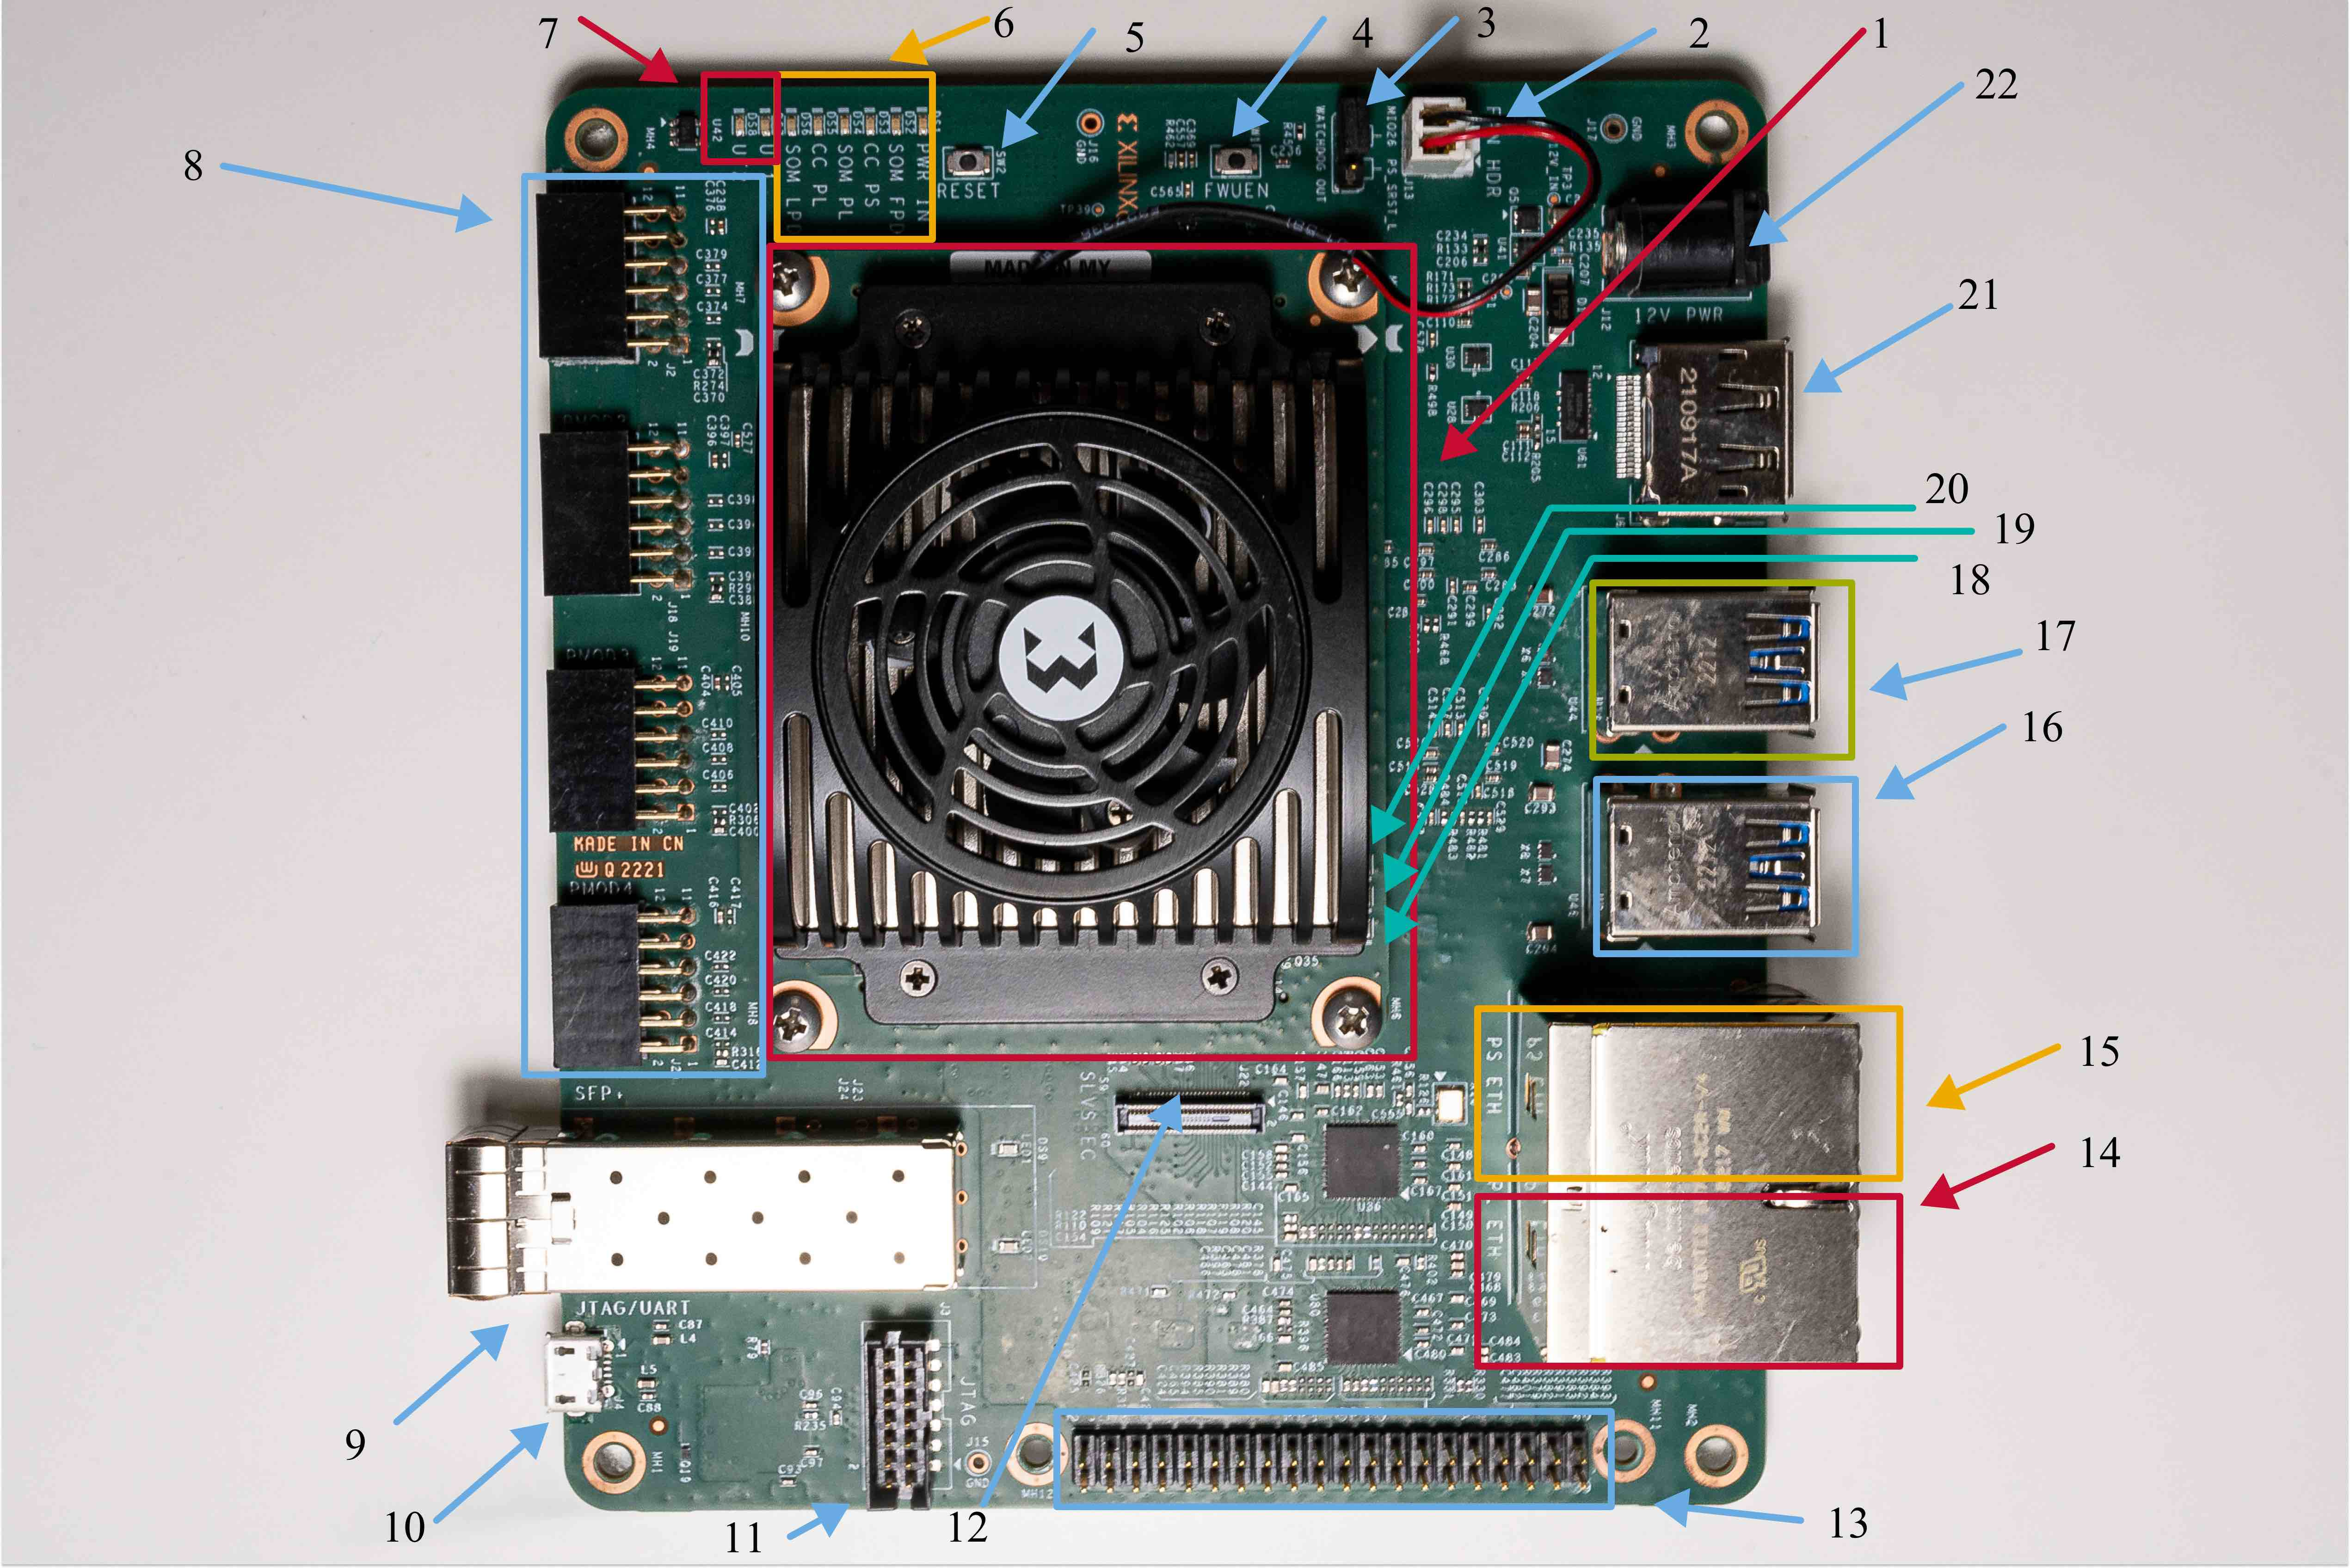
\includegraphics[width=1\textwidth]{src/jpg/xilinx-kria-foto-2-oznacene.jpeg} 
						\caption{Vývojová deska Xilinx Kria KR260 vrchní pohled s~vyznačením komponent.}
						\label{fig:xilinx-kria-foto-2-oznacene}
				\end{figure}


				\begin{figure}[H]
					\centering
						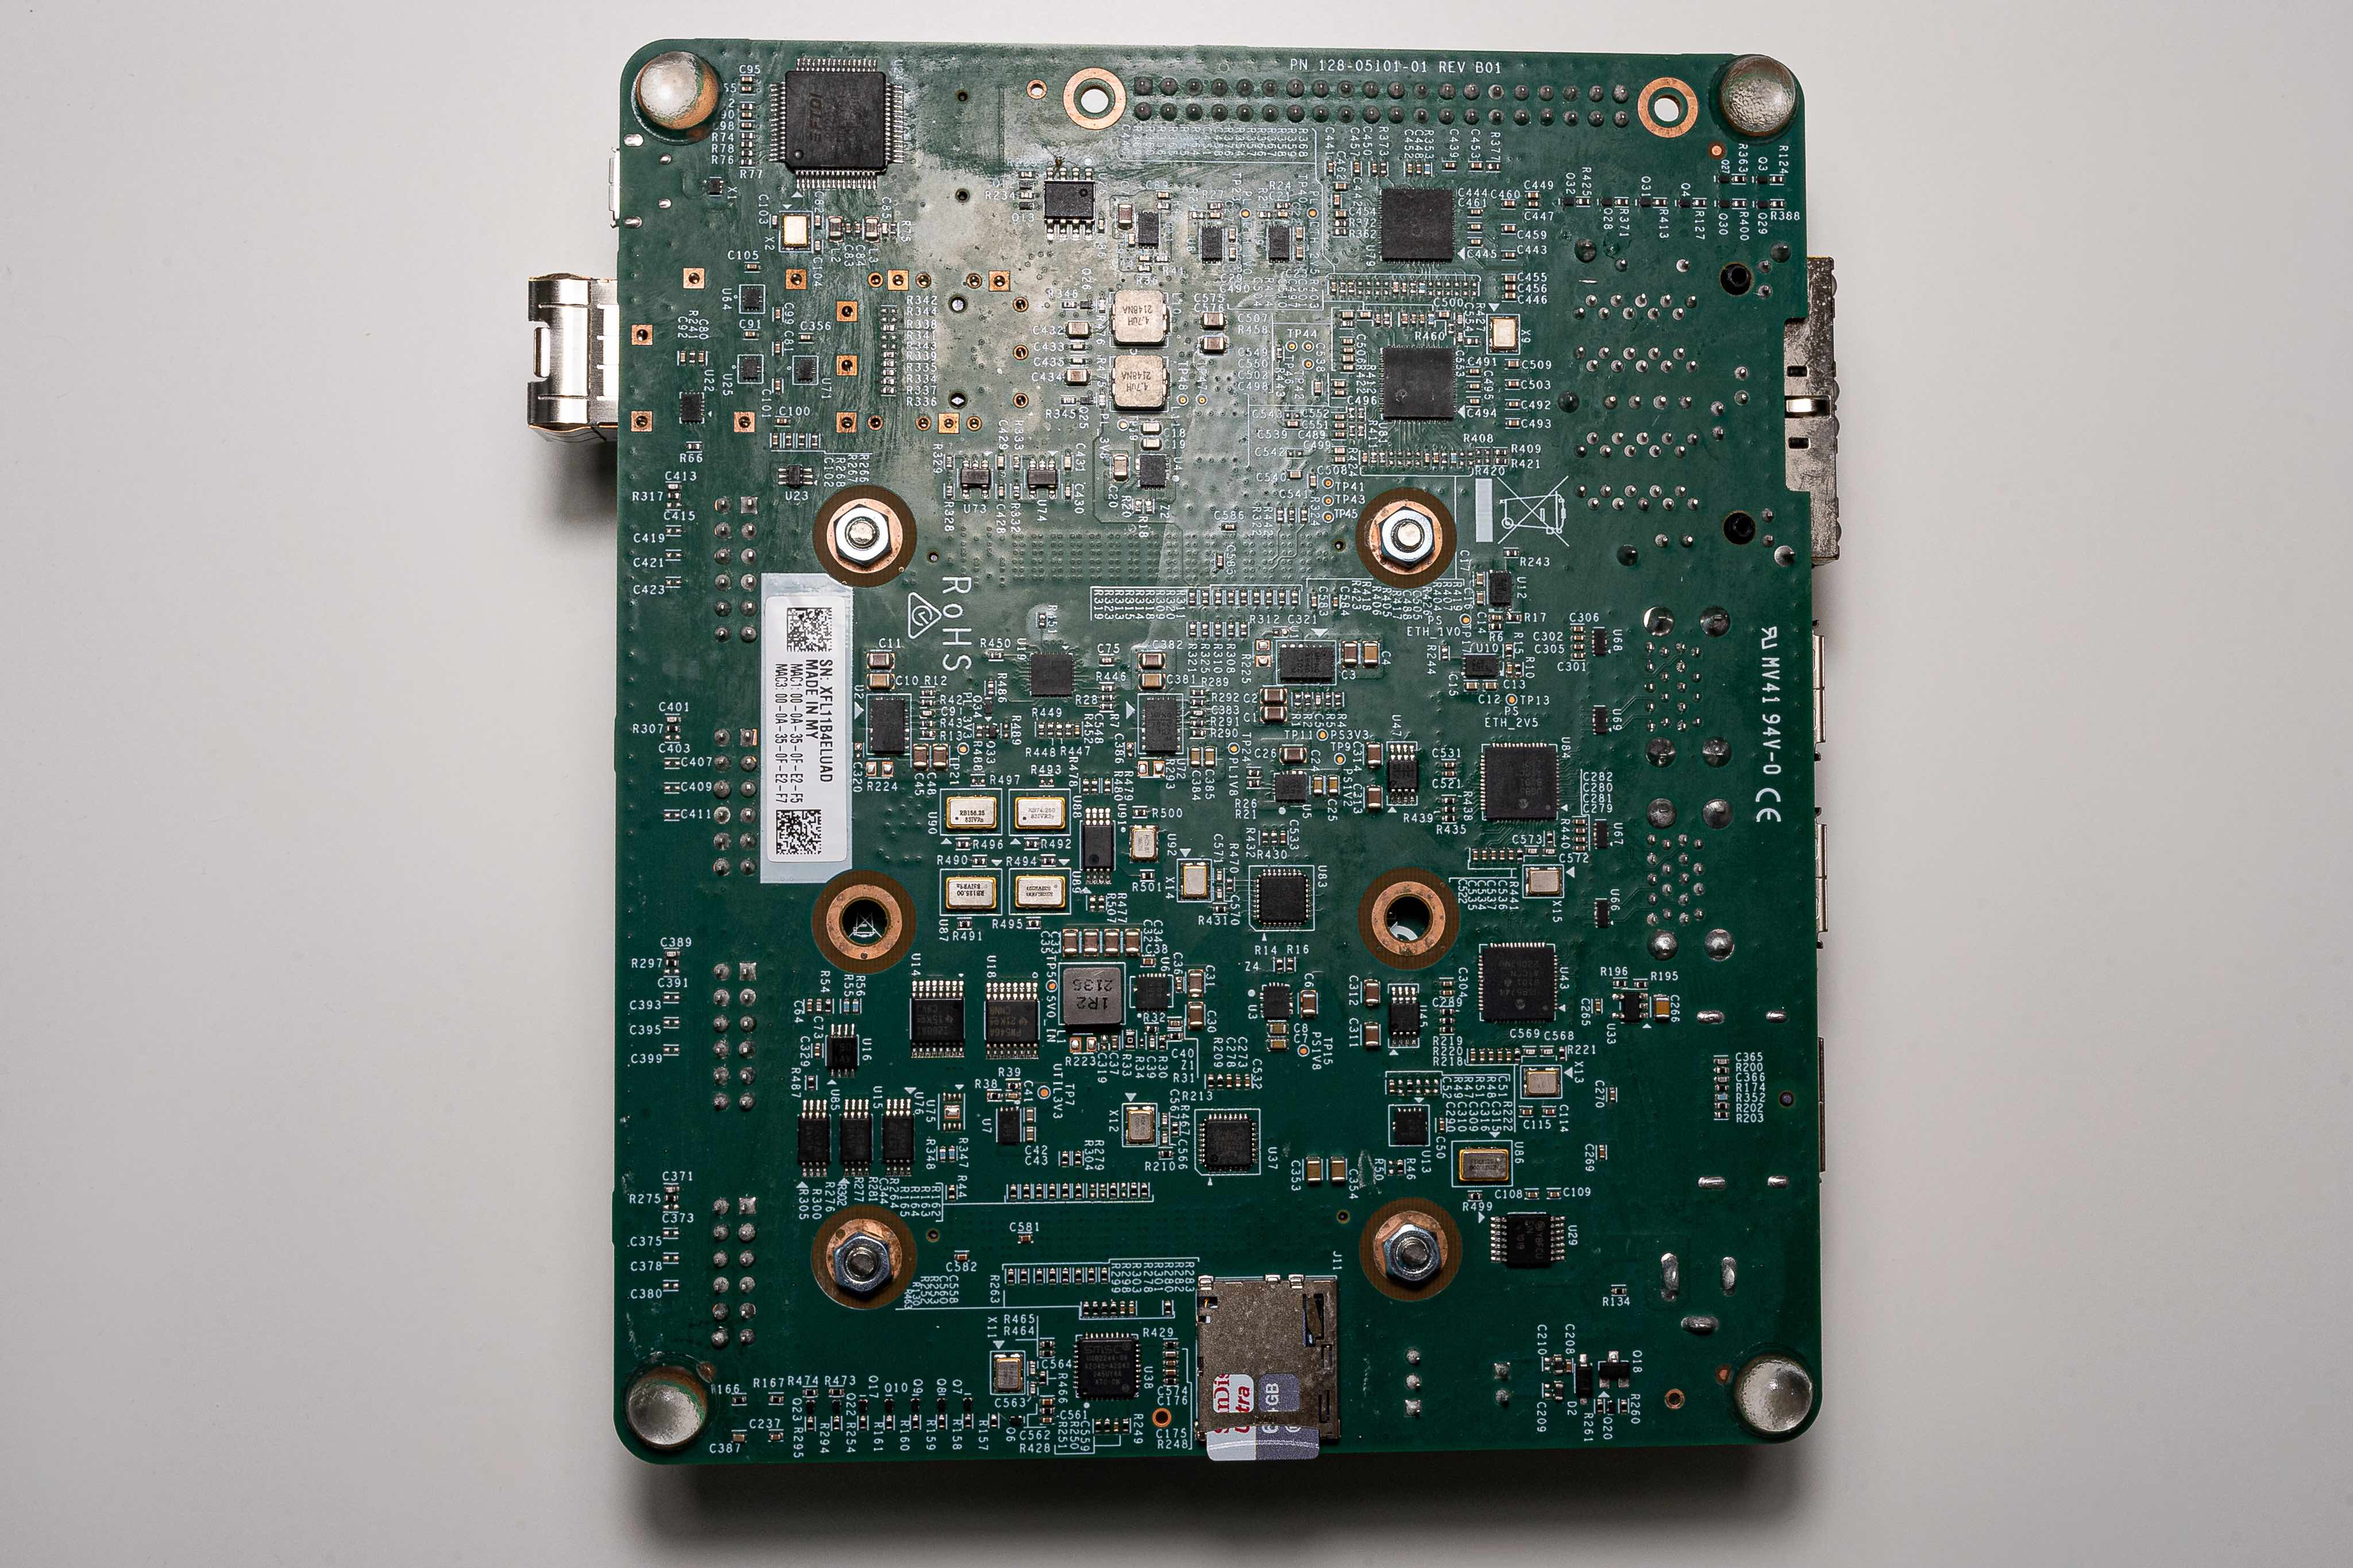
\includegraphics[width=1\textwidth]{src/jpg/xilinx-kria-foto-3.jpeg} 
						\caption{Vývojová deska Xilinx Kria KR260 – spodní pohled.}
						\label{fig:xilinx-kria-foto-3}
				\end{figure}
			
			
				\subsubsection{Dostupné K26 SOM}
					Moduly Kria K26 SOM jsou dostupné v~několika variantách. V~roce 2022 jsou dostupné varianty \textit{Commercial} a \textit{Industrial}. Nadřazeným parametrem dvou hlavních variant jsou varianty SOM s~povoleným nebo zakázaným šifrováním. Varianty se odlišují označením Encryption Disabled (ED) a Encryption Enabled (-). Pokud je šifrování povoleno, je možné šiftovat konfigurační soubory a nebo ve vytvářených aplikacích využívat zabudované \textit{crypto-accelerator} bloky. Encryption Enabled varianty jsou v~některých zemích zakázané a proto je důležité při výběru zboží dbát pokynům prodejce.
					\par Hlavní rozdíly \textit{Commercial} a \textit{Industrial} variant jsou uvedeny v~tab. \ref{tab:xilinx-kria-som-variants}.

					\begin{table}[htbp!]
						\centering
						\caption{Porovnání hlavních parametrů Kria K26 SOM Commercial a Industrial. (informace a značení převzaty z~\cite{kria-k26-som-product-brief})}
						  \vspace*{0.15cm}
						   \resizebox{\textwidth}{!}
							{
								\begin{tabular}{!{\vrule width 2pt} l | c | c !{\vrule width 2pt}}\noalign{\hrule height 2pt}
								parametr & K26 Commercial SOM & K26 Industrial SOM \\
								\noalign{\hrule height 2pt}
								pracovní teplota & 0–85 °C & -40–100 °C\\ \hline
								záruka & 2 roky & 3 roky\\ \hline
								předpokládaná doba životnosti produktu & 5 let & 10 let\\ \hline 
								dostupnost produktu & 10 let & 10 let \\\noalign{\hrule height 2pt}
								\end{tabular}
							}
						\label{tab:xilinx-kria-som-variants}
					\end{table}

					Vývojová deska Xilinx Kria KR260 disponuje dle informací výrobce SOM, který není určen pro nasazení do aplikací (non-production) v~teplotní třídě \textit{Commercial}. \cite{kria-k26-som-ds}
				

			\section{Porovnání představených SoC/SoM platforem pro řízení elektrických pohonů}
			V~předchozích kapitolách byly představeny dvě smysluplné, komerčně dostupné platformy, které je možné využít pro růzznorodé aplikace. Výběr byl zaměřen na SoC a SoM umístěných na vývojových deskách, které je možné využít pro vývoj požadované aplikace. Často po vývoji aplikace následuje uvědomění, jakými periferiemi a vlastnostmi by měla architektura řídící soustavy disponovat. Poté je možné pro velko produkci dané aplikace začít vyvíjet vlastní integraci čipu/modulu na Printed Circuit Board (PCB).\par

			\subsection{Konektivita}
					Aby bylo možné komunikovat s~řízeným zařízením, tudíž vysílat řídící signály a získávat informace o~jeho stavu, je při hodnocení důležitým faktorem možnost připojení.\par
					Obě představené platformy disponují minimálně čtyřmi PMOD konektory s~12 piny (2x U+, 2x GND, 8x I/O), pomocí kterých je možné připojit senzory, převodníky nebo naopak ovládat např. drivery spínacích polovodičových prvků či výkonových polovodičových můstků. PMOD konektorů využívá mnoho komerčně dostupných prvků jako jsou senzory, H můstky nebo také ADC/DAC převodníky.\par
					Dalším důležitým faktorem je připojení Ethernet. Obě desky disponují alespoň jedním konektorem. Xilinx Kria KR260 obsahuje 4 konektory, přičemž dva jsou připojeny přímo do PS a dva do PL. Digilent Zybo disponuje pouze jedním konektorem.\par
					Pro připojení periferií nebo exeterních datových úložišť je možné využít konektor USB. Protože Digilent Zybo Z7 je staršího data vydání, disponuje pouze USB 2.0, zatímco Xilinx Kria KR260 disponuje připojením pomocí USB 3.0.\par
					Pro připojení externího displaye je možné u~Zybo využít D-SUB (VGA) konektor. U~Kria KR260 novější Display Port.\par
					Digilent zybo poté disponuje konektory pro výstup reproduktorů či vstup mikrofonu. Deska KR260 těmito konektory nedisponuje.\par
					Značným přínosem pro konektivitu Kria KR260 je Rraspberry Pi hardware attached on top (HATs) konektor, jež umožňuje připojení rozšiřovacích desek, určených pro Raspberry Pi.\par
					Protože je K26 SOM zaměřen také na AI je možnost připojit k~desce kameru pomocí konektoru SLVS-EC.\par
					Posledním významným konektorem na CC Xilinx Kria je SPF konektor pro připojení optických vláken.

			\subsection{PS a PL}\label{subsec:ps-a-pl}
					Protože je porovnávaná deska Digilent Zybo a Xilinx Kria KR260 různého data vydání a také na jejich pořízení je třeba rozdílných finančních prostředků, odpovídají zdroje pro PS a PL daným cenám.\par
					Jak již bylo zmíněno v~sekci \hyperref[sec:vyvojova-deska-digilent-zybo]{\textit{Vývojová deska Digilent Zybo}}, obsahuje PS použité vývojové deska Digilent Zybo Zynq-7000 dvoujádrový procesor Cortex-A9 s~taktovací frekvencí 650 MHz. Oproti tomu novější PS desky s~Kria K26 SOM obsahuje čtyřjádrový procesor Cortex®-A53 MPCore™ s~taktovací frekvencí až 1,5 GHz. SOM je také doplněn dvoujádrovým real-time dvoujádrovým procesorem Arm Cortex-R5F MPCore s~taktovací frekvencí až 600 MHz. \cite{digilent-zybo-reference-manual}, \cite{kria-k26-som-ds}\par
					Dalším důležitým faktorem jsou zdroje pro PL. Digilent Zybo disponuje pouze 17 600 LUTs. Oproti tomu K26 SOM obsahuje 117 120 LUTs. Novější verze Digilent Zybo desek obsahují novější verze Zynq čipu, který nabízí také 17 600 LUTs (Zybo Z7-10) nebo 53 200 LUTs (Zybo Z7-20). \cite{digilent-zybo-reference-manual}, \cite{kria-k26-som-ds}\par
					Počet LUTs v~této práci má značný vliv na možný rozsah vytvářené aplikace, která je počtem zdrojů (LUTs, Flip-Flops, Block RAM atd.) velmi ovlivněna.\par
					Vlivem omezených zdrojů při realizaci této práce bylo možné i přes optimalizaci C++ kódu (pro dodržení load-compute-store modelu programování \cite{vitis-unified-software-platform-documentation-2022}) akcelerované aplikace (kernel) pro FPGA možné umístit do PL v~Digilent Zybo Z7 pouze matematický I-n model asynchronního motoru, jehož výsledkem byl transformační úhel, složky magnetického toku rotoru $\psi_2^{\alpha \beta}$ a velikost magnetického toku rotoru $| \psi_2 |$. Oproti tomu při využití Kria K26 SOM je možné využít PL pro výpočet I-n modelu stroje, zjednodušeného modelu asynchronního motoru i regulačního zásahu.

			\subsection{Developer Experience}
					V~moderní době, kdy je kladen značný důraz na rychlost vývoje aplikace, je důležitým hodnotícím faktorem developer experience. Tudíž jak je systém konfigurace a vytváření aplikací přívětivý pro vývojáře. V~době vydání Digilent Zybo Z7 byl používán postup vytvoření operačního systému Petalinux již s~pevně daným Device Tree (DT), který byl možné měnit pomocí celkové rekonfigurace a následného opakování celého procesu tvorby systému a aplikace. To přinášelo značné časové prodlevy při ladění aplikace a vytvářeného PL hardware.\par
					Při použití Xilinx Kria K26 SOM je možné při tvorbě systému definovat kostru DT pro PL část, kterou je poté možné do značného rozsahu upravovat pomocí Device Tree Overlay (DTO). Pomocí DTO je možné rekonfigurovat IP vytvářené v~PL. Změnou v~DTO je možné ovlivňovat funkčnost některých IP v~PL při chodu operačního systému Petalinux. Ovšem tyto úpravy mají určitá omezení a je vhodné Device Tree vhodně nakonfigurovat již při vytváření operačního systému Petalinux.\par
					Více informací o~chování a tvorbě DT/DTO, zjištěných při realizaci této práce, je uvedeno v~části \hyperref[subsec:petalinux]{\textit{Petalinux}}.\par
					Digilent pro své výrobky vytvořil „board files“ a „constrains files“, které umožňují snazší konfiguraci PS a PL v~prostředí Vivado. Značným přínosem jsou „constrains files“, které umožňují snazší a rychlejší mapování fyzických pinů vývojové desky k~portům, pinům a rozhraní, vytvářených ve Vivado. Pro vývojovou desku Xilinx Kria KR260 jsou v~repozitáři Vivado již „board files“ zakomponovány. Ovšem oficiální „constrains files“ nejsou od výrobce k~dispozici. Pro mapování pinů je nutné si vyžádat dokumentaci, pomocí které je možné odvodit požadované mapování a „constrains files“ vytvořit. Potřebná dokumentace pro odvození mapování je v~souborech \cite{kria-kr260-starter-kit-cc-schematics} a \cite{kria-k26-som-xdc}.

			\subsection{Aplikace a operační systém}
				Aplikace pro Digilent Zybo je možné převážně vytvářet jako \textit{Bare Metal / Standalone} nebo pro operační systém \textit{Petalinux}. Pro Xilinx Kria je možné využít \textit{Bare Metal / Standalone}, \textit{PetaLinux} a také distribuci operačního systému Linux \textit{Ubuntu}. Protože obě využívané vývojové desky využívají čipu od firmy Xilinx, Inc., je podpora dostupná pro oba čipy relativně srovnatelná. Výrobce na stránkách Wiki podpory zmiňuje, že poskytuje podporu převážně ve formě veřejného fóra na adrese \href{https://support.xilinx.com}{\textit{support.xilinx.com}}. Podpora bude dostupná pro dvě poslední major verze softwaerových nástrojů, které jsou součástí \textit{PetaLinux} a \textit{Xilinx SDK}. \cite{xilinx-wiki-atlassian-embedded-sw-support}\par
				Protože je rodina Kria SOMs modernější než Digilent Zybo, výrobce vytvořil ukázkové akcelerované aplikace, které je možné při využívání operačního systému \textit{Ubuntu} přímo stáhnout z~Kria App Store. \cite{xilinx-appstore-for-kria-soms}
				Oba čipy podporují PREEMPT\_RT Linux Patch. K~tomuto patchi ovšem Xilinx, Inc. neposkytuje žádnou oficiální podporu a je nutné získávat informace přímo od autorů projektu na Wiki stránce \cite{wiki-linux-foundation-real-time-linux} nebo z~omezené podpory pomocí fóra. Více informací o~postupu realizace patche \textit{PetaLinux} je v~sekci \hyperref[subsec:real-time-linux-patch]{\textit{RealTime Linux Patch}}.



\section{Model stroje}
	Jak již bylo představeno v~předchozích částech textu, akcelerované aplikace v~FPGA je možné použít na různé účely. Součástí této práce je realizace akcelerovaného výpočtu matematického modelu stroje. V~této práci bude k~demonstraci funkčnosti využito matematického modelu asynchronního motoru. Asynchronní motor bude modelován pro řízení pomocí $I$-$n$ modelu a pro simulační účely pomocí zjednodušeného modelu, zanedbávající některé jevy.\par
	Pokud FPGA obsahuje dostatečné množství zdrojů, je možné realizovat akcelerovaný výpočet „kompletního“ matematického modelu, ve kterém např. dochází k~simulovanému generování vstupního napětí, jehož popis pomocí rovnic je představen v~části \hyperref[subsec:matematicky-popis-kompletniho-modelu-stroje]{\textit{Matematický popis „kompletního“ modelu stroje}}. V~části \hyperref[subsec:ps-a-pl]{\textit{PL a PS}} je uvedeno, že vlivem omezených zdrojů je možné realizovat v~Digilent Zybo Z7 pouze $I$-$n$ model stroje. Ostatní výpočty je nutné realizovat v~PS. V~Xilinx Kria K26 je díky většímu množství zdrojů možné realizovat větší část modelu v~PL a pomocí PS řešit pouze konfiguraci, řízení procesu akvizice dat apod.\par
	%% mám se v této celé kapitole více rozepsat o odvození modelu ASM
	%% schéma, princip činnosti, napěťové a tokové rovnice
	%% v optimalizace/úpravě modelu pro jazyk C++ mám se rozepsat o numerických metodách? RK4 bych použil
	%% kde prosím naleznu odvození těch rovnic na model stator proud rotor tok
	% clarkovy transformace - popsat
	% goniometrické funkce jsou v pure c++ v knihovně cmath, ve vitis jsou v hls_math.h
	% https://docs.xilinx.com/r/en-US/ug1399-vitis-hls/Vitis-HLS-Math-Library
	\subsection{Představení stroje}
	\subsection{Matematický popis „kompletního“ modelu stroje}\label{subsec:matematicky-popis-kompletniho-modelu-stroje}
	\begin{minipage}[t]{0.47\textwidth}
        \vspace{\baselineskip}
        \begin{table}[H]
            \caption{Štítkové údaje stroje.}
            \centering
                \begin{tabular}{!{\vrule width 2pt} c | c !{\vrule width 2pt}}\noalign{\hrule height 2pt}
                    $P_\text{n}$ & 12 kW \\ \hline
                    $U_\text{n}$ & 380 V~\\ \hline
                    $I_\text{n}$ & 22 A\\ \hline
                    $n_\text{n}$ & 1460 min$^{-1}$ \\ \hline
                    $f_\text{n}$ & 50 Hz \\ \hline
                    $\cos(\varphi_\text{n})$ &  0.8 \\ \hline
                    $p_\text{p}$ & 2 \\ \noalign{\hrule height 2pt}
                \end{tabular}     
            \label{tab:stitkove-udaje}
        \end{table}
        \end{minipage}% --- important, otherwise it wont be so nice
        \hfill
        \begin{minipage}[t]{0.47\textwidth}
            \vspace{0pt}
            \begin{table}[H]
                \caption{Změřené parametry stroje.}
                \centering
                    \begin{tabular}{!{\vrule width 2pt} c | c !{\vrule width 2pt}}\noalign{\hrule height 2pt}
                        $R_\text{1}$ & 370 m$\Omega$ \\ \hline
                        $R_\text{2}$ & 225 m$\Omega$ \\ \hline
                        $L_{1\sigma}$ & 2,27 mH \\ \hline
                        $L_{2\sigma}$ & 2,27 mH \\ \hline
                        $L_\text{m}$ & 82,5 mH \\ \hline
                        $L_{1}$ & 84,77 mH \\ \hline
                        $L_{2}$ & 84,77 mH \\ \hline $J$ & 0,4 kg$\cdot$m$^{2}$ \\ \noalign{\hrule height 2pt}
                    \end{tabular}     
                \label{tab:zmerene-parametry-stroje}
            \end{table}
        \end{minipage}

        \vspace*{1cm}
Kde $P_\text{n}$ (W) je jmenovitý výkon stroje, $I_\text{n}$ (A) je jmenovitý fázový proud stroje (efektivní hodnota), $U_\text{n}$ (V) je jmenovité sdružené napájací napětí stroje, $f_\text{n}$ (Hz) je jmenovitá napájecí frekvence stroje, $\cos(\varphi_\text{n})$ (-) je jmenovitý účinník stroje, $n_\text{n}$ (min$^{-1}$) jsou jmenovité otáčky stroje, $p_\text{p}$ (-) je počet polpárů stroje, $R_1$ ($\Omega$), resp. $R_2$ ($\Omega$) je statorový, resp. rotorový odpor, $L_{1\sigma}$ (H), resp. $L_{2\sigma}$ (H) je statorová, resp. rotorová rozptylová  indukčnost stroje, $L_\text{m}$ (H) je magnetizační indukčnost stroje, $L_1$ (H), resp. $L_2$ (H) je statorová, resp. rotorová indukčnost, $J$ (kg$\cdot$m$^{2}$) je moment setrvačnosti hřídele.\par
V~případě tvorby modelu, je využit model založen na výpočtu složek vektorů statorového proudu $\underline{i_1}$ a rotorového toku $\underline{\psi_2}$ v~souřadnicovém systému $\alpha\beta$ spojeném se statorem. Tudíž při použití $\omega_k = 0$. Bude volena konstanta $K = 2/3$. Poté bude stavový popis systému vypadat následovně.

\begin{equation}
    \frac{\dd{}}{\dd{t}}
    \begin{bmatrix}
        i_{1\alpha}\\
        i_{1\beta}\\
        \psi_{2\alpha}\\
        \psi_{2\beta}
    \end{bmatrix}
    =
    \begin{bmatrix}
        -\frac{R_2 L_\text{m}^{2} + L_2^2 R_1}{\sigma L_1 L_2^2} & 0 & \frac{L_\text{m} R_2}{\sigma L_1 L_2^2} & \frac{L_\text{m}}{\sigma L_1 L_2} \omega\\
        0 & - \frac{R_2 L_\text{m}^2 + L_2^2 R_1}{\sigma L_1 L_2^2} & - \frac{L_\text{m}}{\sigma L_1 L_2} \omega & \frac{L_\text{m} R_2}{\sigma L_1 L_2^2}\\
        \frac{L_\text{m} R_2}{L_2} & 0 & - \frac{R_2}{L_2} & -\omega\\
        0 & \frac{L_\text{m} R_2}{L_2} & \omega & -\frac{R_2}{L_2}
    \end{bmatrix}
    \begin{bmatrix}
        i_{1\alpha}\\
        i_{1\beta}\\
        \psi_{2\alpha}\\
        \psi_{2\beta}
    \end{bmatrix}
    +
    \begin{bmatrix}
        \frac{1}{\sigma L_1} & 0\\
        0 & \frac{1}{\sigma L_1}\\
        0 & 0\\
        0 & 0
    \end{bmatrix}
    \begin{bmatrix}
        u_{1\alpha}\\
        u_{1\beta}
    \end{bmatrix}.
\end{equation}
Stavový popis je vhodné doplnit o~další rovnice, jež budou v~simulaci využity.

\begin{equation}
    M = \frac{3}{2} p_\text{p} \frac{L_\text{m}}{L_2} (\psi_{2\alpha} i_{1\beta} - \psi_{2\beta} i_{1\alpha}),
\end{equation}

\begin{equation}
    M - M_\text{z} = J \frac{\dd{\Omega}}{\dd{t}},
\end{equation}
\begin{equation}
    \omega = p_\text{p} \Omega,
\end{equation}
kde $\sigma = 1 - L_\text{m}^{2}/(L_1 L_2)$ (-) je tzv. rozptyl, $i_{1\alpha}$ (A) a $i_{1\beta}$ (A) jsou složky vektoru statorového proudu $\underline{i_1}$ (A), $\psi_{2\alpha}$ (Wb) a $\psi_{2\beta}$ (Wb) jsou složky vektoru rotorového magnetického toku $\underline{\psi_2}$ (Wb), $u_{1\alpha}$ (V) a $u_{1\beta}$ (V) jsou složky statorového napětí $\underline{u_1}$ (V), $p_\text{p}$ (-) je počet polpárů stroje, $\omega$ (s$^{-1}$) je elektrická úhlová rychlost hřídele, $\Omega$ (s$^{-1}$) je mechanická úhlová rychlost hřídele, $M$ je vnitřní elektromechanický moment stroje a $M_\text{z}$ (Nm) je moment zátěžný.

	\subsection{I-n model asynchronního motoru}
		Jak již bylo v~předcházejících částech zmíněno, pokud není k~dispozici dostatečný počet LUTs pro výpočet kompletního matematického modelu, je možné využít PL na výpočet např. proudově-otáčkového, resp. $I$-$n$ modelu a regulační procesy realizovat v~PS.\par
		Popis $I$-$n$ modelu vychází ze základních rovnic, popisující asynchronní motor, uvedených např. v~\cite{kobrle-elektricke-pohony} (rovnice jsou upraveny a přeznačeny dle moderních konvencí ale význam zůstává zachován). V~teorii prostorových vektorů je možné tedy psát soustavu rovnic

		\begin{equation}
			\underline{u_{1}^{k}} = R_1 \underline{i_{1}^{k}} + \frac{\dd{\underline{\psi_1^{k}}}}{\dd{t}} + \text{j} \omega_k \underline{\psi_1^{k}},
		\end{equation}
		\begin{equation}
			\underline{u_{2}^{k}} = R_2 \underline{i_{2}^{k}} + \frac{\dd{\underline{\psi_2^{k}}}}{\dd{t}} + \text{j} (\omega_k - \omega) \underline{\psi_2^{k}},
		\end{equation}
	
		\begin{equation}
			\underline{\psi_1^{k}} = L_1 \underline{i_1^{k}} + L_\text{m} \underline{i_2^{k}},
		\end{equation}
	
		\begin{equation}
			\underline{\psi_2^{k}} = L_2 \underline{i_2^{k}} + L_\text{m} \underline{i_1^{k}},
		\end{equation}

		kde $\underline{u_{1}^{k}}$ (V) je prostorový vektor statorového napětí, $\underline{u_{2}^{k}}$ (V) je prostorový vektor rotorového napětí, $\underline{i_{1}^{k}}$ (A) je prostorový vektor statorového proudu, $\underline{i_{2}^{k}}$ (A) je prostorový vektor rotorového proudu, $\underline{\psi_1^{k}}$ (Wb) je prostorový vektor magnetického toku statoru, $\underline{\psi_2^{k}}$ (Wb) je prostorový vektor magnetického toku rotoru, $\omega$ (s$^{-1}$) je úhlová rychlost otáčení rotoru, $\omega_k$ (s$^{-1}$) je úhlová rychlost otáčení použitého souřadnicového systému, $R_1$ ($\Omega$), resp. $R_2$ ($\Omega$) je rezistivita statorového, resp. rotorového vinutí, $L_1$ (H), resp. $L_2$ (H) je statorová, resp. rotorová indukčnost a $L_\text{m}$ (H) je hlavní magnetizační indukčnost.\par
		I-n model vychází z~předpokladu, že otáčivá úhlová rychlost souřadnicového systému $\omega_k$ = 0 a tudíž model bude odvozován v~souřadnicovém systému spojeným se statorem (souřadnicový systém $\alpha \beta$). Po vzolení daného souřadnicového systému pro soustavu rovnic platí

		\begin{equation}
			\underline{u_{1}^{\alpha \beta}} = R_1 \underline{i_{1}^{\alpha \beta}} + \frac{\dd{\underline{\psi_1^{\alpha \beta}}}}{\dd{t}},
		\end{equation}
		\begin{equation}\label{eq:alphabeta-napeti-rotor-rovnice-i-n-model}
			\underline{u_{2}^{\alpha \beta}} = R_2 \underline{i_{2}^{\alpha \beta}} + \frac{\dd{\underline{\psi_2^{\alpha \beta}}}}{\dd{t}} - \text{j} \omega \underline{\psi_2^{\alpha \beta}},
		\end{equation}
	
		\begin{equation}
			\underline{\psi_1^{\alpha \beta}} = L_1 \underline{i_1^{\alpha \beta}} + L_\text{m} \underline{i_2^{\alpha \beta}},
		\end{equation}
	
		\begin{equation}\label{eq:alphabeta-tok-rotor-rovnice-i-n-model}
			\underline{\psi_2^{\alpha \beta}} = L_2 \underline{i_2^{\alpha \beta}} + L_\text{m} \underline{i_1^{\alpha \beta}}.
		\end{equation}

		V~případě řízení asynchronního motoru s~kotvou nakrátko orientovaného na rotorový tok je dále z~rovnice \ref{eq:alphabeta-tok-rotor-rovnice-i-n-model} vyjádřen prostorový vektor $\underline{i_2^{\alpha \beta}}$, který je dále dosazen do upravené rovnice \ref{eq:alphabeta-napeti-rotor-rovnice-i-n-model}, u~které je přepokládáno, že $\underline{u_{2}^{\alpha \beta}}$ = 0.
		Výsledná diferenciální rovnice pro prostorový vektor rotorového magnetického toku je

		\begin{equation}
			\frac{\dd{\underline{\psi_{2}^{\alpha \beta}}}}{\dd{t}} = \frac{R_2}{L_2}L_\text{m} i_1^{\alpha \beta} + j \omega \underline{\psi_2^{\alpha \beta}} - \frac{R_2}{L_2} \underline{\psi_2^{\alpha \beta}}.
		\end{equation}

		Rozepsáním představené diferenciální rovnice do reálné a imaginární složky vznikne soustava diferenciálních rovnic, kterou je třeba řešit.

		\begin{equation}
			\begin{gathered}
				\frac{\dd{\underline{\psi_{2\alpha}}}}{\dd{t}} = \frac{L_\text{m} R_2}{L_2} i_{1\alpha} - \frac{R_2}{L_2} \psi_{2\alpha} - \omega \psi_{2\beta},\\\frac{\dd{\underline{\psi_{2\beta}}}}{\dd{t}} = \frac{L_\text{m} R_2}{L_2} i_{1\beta} - \frac{R_2}{L_2} \psi_{2\beta} + \omega \psi_{2\alpha}.
			\end{gathered}
		\end{equation}


\section{Použité nástroje pro vývoj aplikace pro PS a PL}
V~této části jsou představeny jednotlivé nástroje, využívané při tvorbě programu pro PS a akcelerované aplikace (kernelu) realizované na PL. Je důležité zmínit, že na v PS je skutečně spouštěn zkompilovaný program vytvářený pomocí jazyka C, C++ nebo Python. Na PL je ovšem vytvořen HW, který reprezentuje myšlené algoritmy aplikace. Tento HW je popisován pomocí nízkoúrovňových jazyků, do kterých je algoritmus převeden v HLS z jazyka C. Není tudíž korektně správné mluvit o~tom, že se vytváří program pro FPGA. Z toho důvodu bude v~této práci používáno označení pro vytváření HW na PL \textit{vytváření kernelu} (creation of the kernel). Označení \textit{kernel} je myšleno v odlišném významu než je využíváno v části \hyperref[subsec:real-time-linux-patch]{\textit{RealTime Linux Patch}}.\par
	% Také jsou v~této části představeny postupy využívání vývojových nástrojů, které vedou k~úspěšné tvorbě aplikace.\par
Tvorba akcelerované aplikace může být obecně prováděna více způsoby. Tento způsob závisí na použitém vývojovém nástroji pro daný HW. V~této práci je využíváno SOM od firmy Xilinx, proto je výhodné využívat již připravené nástroje, které umožní snazší vývoj SW, tvorbu HW a přípravu systému na SOM.\par
	Veškerý používaný SW v~této práci od firmy Xilinx je po registraci volně dostupný ke stažení na \cite{xilinx-downloads}.
		\subsection{Xilinx Vivado}\label{subsec:xilinx-vivado}
			Xilinx Vivado je nástroj, používaný pro tvorbu HW architektury, resp. platformy, pro kterou bude v další části postupu možné vytvořit akcelerovanou aplikaci. Ve Vivado je možné tvořit HW návrh, převeditelný do HDL, který bude spustitelný v~PL bez použití Vitis HLS. Pro vývojáře HW pro FPGA může sloužit i jako jediný vývojářský nástroj.\par
			Se znalostí VHDL je možné ve Vivado vytvářet požadované HW konstrukce, ovšem tvorba těchto konstrukcí ve Vivado je relativně náročnou záležitostí není předmětem této práce, ale je nevyhnutelnou součástí výzkumu využití těhto platforem pro řízení elektrických pohonů.\par
			Xilinx Vivado je součástí instalačního balíčku \textit{Xilinx Unified Installer}, dostupného z~\cite{xilinx-downloads}. Součástí balíčku verze 2022.2 SFD je také nástroj \hyperref[subsec:xilinx-vitis]{\textit{Xilinx Vitis}}. Je doporučeno instalovat oba tyto programy a vyvarovat se oddělené instalace, jež může přinášet problémy se vzájemnou i zpětnou kompatibilitou jednotlivých nástrojů.
		\subsection{Xilinx Vitis}\label{subsec:xilinx-vitis}
		Xilinx Vitis je nástroj, který slouží k~vytváření akcelerovaných aplikací na zařízení firmy Xilinx. Tento nástroj obsahuje základní vrstvu s~názvem Xilinx Vitis HLS, která slouží jako jádro převodu vytvářených aplikací v~C, C++, OpenCL do RTL. V~programu Xilinx Vitis bude vytvářena největší část aplikace, proto je vhodné nastínit postup, jakým Vitis pracuje.
		\par
		Nejprve je vytvořen tzv. „host program“ bežící na PS, který je vyvíjen v~C/C++ jazyku (popř. Python), používající Xilinx Runtime (XRT) Application Programming Interface (API). Tento program je následně kompilován pomocí g++ kompilátoru, který vytvoří spustitelný soubor pro procesor. Tento host program komunikuje s~akcelerovanou částí aplikace (kernel), umístěným v~PL v~FPGA. Blok \textit{ARM x86 host Application Compilation} naznačuje, jakým způsobem je vytvářena aplikace pro host procesor. \cite{vitis-unified-software-platform-documentation-2022}\par
		Poté Vitis HLS compiler přeloží C/C++ zdrojový kód pro kernel do register transfer level (RTL) (úrovně registrů). Produkty této kompilace mají příponu „.xo“ (Xilinx Object) a mohou být spojovány do binárního souboru s~příponou „.xclbin“ pomocí Vitis linkeru. Souborem \textit{kernel.xclbin} je poté možné nakonfigurovat PL.\cite{vitis-unified-software-platform-documentation-2022}\par
		Na obr. \ref{fig:vitis-development-flow} je blokově znázorněn postup tvorby spustitelné aplikace v~programu Vitis. Tento diagram předpokládá, že již byla vytvořena HW platforma ve Vivado a PetaLinux systém.\par
		Produkty větve programu pro PS a konfigurace pro PL je po jejich dokončení možné použít v daném heterogenním systému. Host program zařídí nakonfigurování PL pomocí souboru \textit{kernel.xclbin} a následné zpracování výsledků. Blok s~názvem \textit{Running the Application} je kompletně vykonáván v~prostředí PetaLinux v~simulátoru (QEMU) nebo na fyzickém zařízení (vývojová deska).
		\begin{figure}[htbp!]
			\centering
			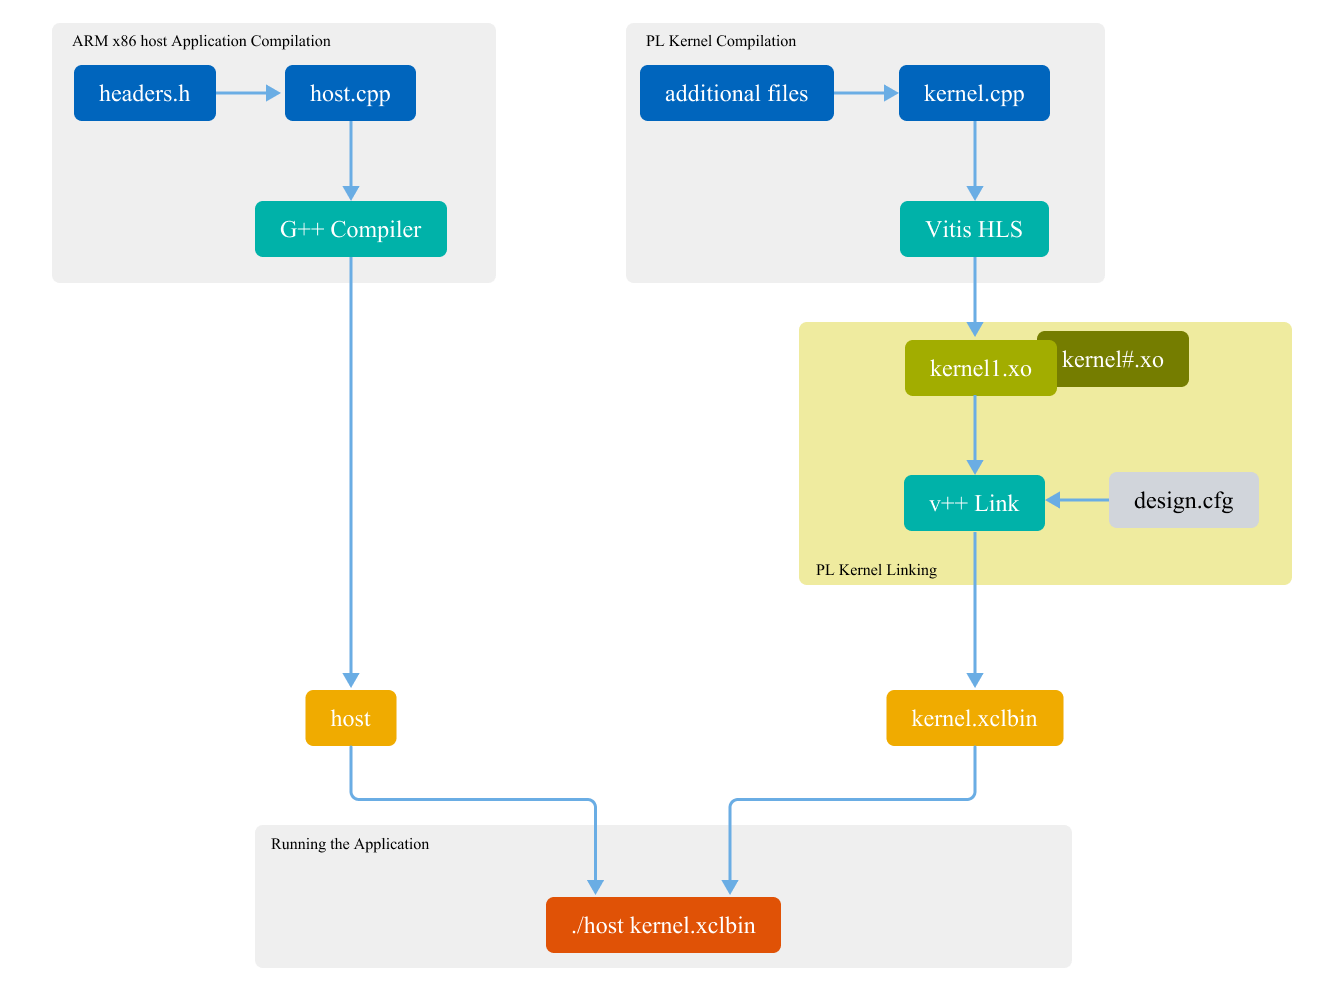
\includegraphics[width=1\textwidth]{src/png/vitis-development-flow.png}
			\caption{Blokový diagram tvorby spustitelné aplikace v~prostředí Vitis. (převzato z~\cite{vitis-unified-software-platform-documentation-2022}, upraveno)}
			\label{fig:vitis-development-flow}
		\end{figure}
		
		\subsection{PetaLinux Tools}\label{subsec:petalinux-tools}
			PetaLinux Tools je nástroj, který slouží k~vytvoření systému PetaLinux, který bude spuštěn na PS v daném SOM nebo SoC. Z~tohoto systému je poté možné spouštět navazující programy host a kernel.\par
			PetaLinux poskytuje distribuci systému Linux, který uživatel před tvorbou aplikace pomocí \hyperref[subsec:xilinx-vitis]{Xilinx Vitis} využívá k~tomu, aby vytvořil operační systém, na kterém bude možné spuštět dané akcelerované aplikace. Tento systém je možné nakonfigurovat dle požadavků aplikace. Při tvoření tohoto systému je možné konfigurovat jádro systému (kernel), balíčky, které budou do systému nainstalovány, vytvořit uživatele systému nebo vybrat, kde v~paměti bude systém umístěn (RAM, SD karta apod.). \cite{xilinx-petalinux}\par
			PetaLinux Tools mohou sloužit k~debuggingu a virtualizaci systému pomocí QEMU. V~případě tvorby systému, který je konfigurovaný uživatelem, je třeba postupovat obezřetně a dodržovat nastavené postupy konfigurace, protože v případě chyby je nutné překonfigurovat chybnou část nebo někdy kompletní build. Tvorba PetaLinux systému je časově náročný postup, u něhož je problematický debugging.\par
			Pro funkční instalaci PetaLinux Tools je nutné disponovat nainstalovanými správnými verzemi systémových a aplikačních balíků, které jsou nutnou prerekvizitou tvorby PetaLinux pro PS. Požadavky na balíky je možné nalézt při nahlédnutí do dokumentace \cite{petalinux-tools-documentation-2022} (UG1144) dané instalované verze PetaLinux Tools. V sekci \textit{Installation Reguirements} se nachází odkaz označený \textit{PetaLinux <version> Release Notes}, který ve spodní čásit obsahuje stáhnutelný soubor \textit{<version>\_PetaLinux\_Package\_List.xlsx}, který obsahuje požadované balíky a jejich verze. Bez použití podporovaných balíků by neprracoval nástroj PetaLinux Tools správně.

		\subsection{RealTime Linux Patch}\label{subsec:real-time-linux-patch}
			Protože operační systém Linux nebyl původně vytvářen pro využití v embedded systémech, ale v obecných zařízeních jako jsou servery a stolní počítače, nebyl tento systém vhodný pro řešení úloh v reálném čase. Proto se objevila snaha upravit tento systém takovým způsobem, aby jej bylo možné využívat v real time systémech.\par
			Real time systémy je obvykle možné rozdělit do jednotlivých úrovní podle časových požadavků systému v reálném čase na:
			\begin{itemize}
				\item \textbf{Soft Real Time} – aplikace, ve které je hlavním parametrem kvalita výsledků, pokud v některých případech nedojde k dodržení časových omezení jednotlivých úkonů, nemá tato chyba vliv na zdraví člověka nebo stav majetku,
				\item \textbf{Firm Real Time} – pokud v aplikaci nedojde k dodržení časových omezení výpočtů, je výsledek daného výpočtu považován za neplatný a nelze jej použít,
				\item \textbf{Hard Real Time} – v aplikaci je zakázáno nedodržení časových omezení, kdyby došlo k překročení pevně daných časových rámců, může vzniklá situace vést k ohrožení lidských životů nebo stavu majetku.
			\end{itemize}
			V \cite{the-real-time-linux-kernel-survey-on-preempt-rt} jsou představeny původní přístupy, kdy pro dodržení časových omezení a tzv. „preemptibility“ (přerušitelnosti vykonávaného vlákna) byl využit \textit{cokernel}.\par
			Moderní způsob spočívá v aplikování Linux patch pro danou verzi kernelu (pojmem kernel v tomto případě není myšlena akcelerovaná aplikace, ale jádro operačního systému Linux), kdy není přidávaná do systému další vrstva jádra, ale původní jádro je upravováno. Úpravy spočívají ve změně některých přístupů funkčnosti jádra a přerušení. Tento patch se obecně nazývá \textit{PREEMPT\_RT} a o začlenění jeho principů do mainline kernelu je dlouhodobě usilováno. \cite{the-real-time-linux-kernel-survey-on-preempt-rt}\par
			Popis state-of-art \textit{PREEMPT\_RT} je popsán v \cite{the-real-time-linux-kernel-survey-on-preempt-rt}. V této práci je patch využit pro získání co největší přerušitelnosti jádra, tudíž aby byl kernel \textit{FULLY PREEMPTIBLE}. Pokud by tomu tak nebylo, nebyly by výsledky simulací matematických modelů při použití PL a PS konzistentní. Pokud je využívána architektura simulace, naznačená na obr. \ref{fig:rt-simulation-graph}, dojde při opakovaném spuštění aplikace s vysokou pravděpodobností k získání znehodnocených výsledků, které není možné použít. Při spuštění aplikace se tento problém projeví nevalidními výsledky, které neodpovídají žádnému ze zadaných parametrů. Po opakovaném spuštění aplikace je možné získat validní výsledky, ovšem četnost, kdy dochází k získání nevalidních výsledků, je značně vysoká.

			\begin{figure}[H]
				\centering
					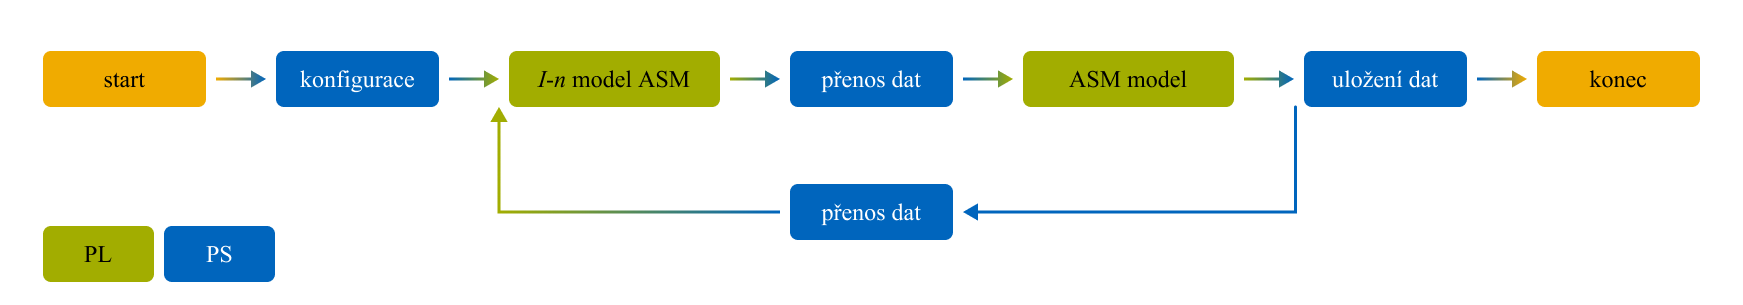
\includegraphics[width=1\textwidth]{src/png/rt-simulation-graph.png} 
					\caption{Graf prováděné simulace při testování PREEMPT\_RT Linux Patch.}
					\label{fig:rt-simulation-graph}
			\end{figure}
			
			\fbar
			\subsubsection{Postup aplikace PREEMPT\_RT patch}
				Patch je možné aplikovat několika způsoby. V této práci byl aplikován při fázi tvoření PetaLinux systému pomocí úpravy konfiguračních souborů build procesu.\par
				Pro bezproblémové aplikování patche je vhodné nejdříve vytvořit \textit{build} PetaLinux systému bez aplikovanání patch souboru s minimální konfigurací a po úspěšném vytvoření systému patch aplikovat a build proces opakovat. Pro funkční aplikaci patch souboru je nutné znát verzi jádra PetaLinux, na který bude aplikován. Označení verze je možné získat z \texttt{Makefile} souboru umístěného v cestě naznačené v kódu \ref{lst:petalinux-kernel-makefile-path}, kde \texttt{<petalinux-project>} je označení pro kořenový (root) adresář PetaLinux projektu, který je tvořen.

				\begin{lstlisting}[language={sh}, caption={Cesta Makefile souboru, ze kterého je možné získat označení verze jádra systému PetaLinux.}, label= {lst:petalinux-kernel-makefile-path}]
<petalinux-project>/build/tmp/work-shared/xilinx-k26-kr/kernel-source/Makefile\end{lstlisting}
				Protože je zmiňovaný \texttt{Makefile} soubor rozměrný a pro určení verze kernelu je signifikantní pouze jeho úvodní část, je v kódu č. \ref{lst:petalinux-makefile-kernel-version} vynechána podstatná část souboru, která není pro aplikování patche podstatná.

				\begin{lstlisting}[language={make}, caption={Významná část Makefile souboru pro určení verze jádra PetaLinux.}, label= {lst:petalinux-makefile-kernel-version}]
# SPDX-License-Identifier: GPL-2.0
VERSION = 5
PATCHLEVEL = 15
SUBLEVEL = 36
EXTRAVERSION =
NAME = Trick or Treat
...\end{lstlisting}
				
				Z kódu \ref{lst:petalinux-makefile-kernel-version} je možné vyčíst, že je třeba využít patch pro verzi \textit{5.15.36}. Pokud není možné informaci ohledně verze jádra linuxu dohledat, je možné vytvořit PetaLinux obvyklým způsobem, vytvořit obraz systému, ten nahrát na SD kartu, provést spuštění systému na vývojové desce a po úspěšném přihlášení do systému vyvolat příkaz \texttt{uname -a} a dle uvedených informací odvodit verzi jádra.\par
				Poté je z adresy \href{https://cdn.kernel.org/pub/linux/kernel/projects/rt/}{\textcolor{ctublue}{https://cdn.kernel.org/pub/linux/kernel/projects/rt/}} možné stáhnout patch pro zjištěnou verzi jádra. V této práci byl využit patch pro Petalinux 2022.2 umístěný v cestě \texttt{5.15/older/patch-5.15.36-rt41.patch.gz}.\par
				Dalším krokem je extrahovaný soubor \texttt{patch-5.15.36-rt41.patch} přenést do složky \texttt{<petalinux-project>/project-spec/meta-user/recipes-kernel/linux/linux-xlnx/}. Build proces musí následně mít informaci o umístění daného souboru, proto je vyžadováno aby do souboru \texttt{<petalinux-project>/project-spec/meta-user/recipes-kernel/linux/linux-xlnx\_\%.bbappend} zapsat na poslední řádek příkaz \texttt{SRC\_URI:append = " file://patch-5.15.36-rt41.patch"}, kde \texttt{patch-5.15.36-rt41.patch} je název patch souboru. Ukázka \texttt{linux-xlnx\_\%.bbappend} souboru, využitého v této práci je v kódu \ref{lst:petalinux-patch-bbbappend}. Jak je vidět, soubor obsahuje informace o různých konfiguračních souborech pro tvorbu jádra Linux systému. Šestý řádek označuje uživatelskou konfiguraci, pomocí data, kdy byla vytvořena.

				\begin{lstlisting}[language={sh}, caption={Ukázka konfiguračního souboru pro aplikování Linux patch souboru.}, label= {lst:petalinux-patch-bbbappend}]
FILESEXTRAPATHS:prepend := "${THISDIR}/${PN}:"

SRC_URI:append = " file://bsp.cfg"
KERNEL_FEATURES:append = " bsp.cfg"
SRC_URI:append = " file://patch-5.15.36-rt41.patch"
SRC_URI += "file://user_2023-04-07-11-32-00.cfg"\end{lstlisting}

				Aby došlo k aplikování změn, vyvolaných RT patch souborem je nutné během build procesu provést určité změny v konfiguraci vytvářeného PetaLinux projektu. (postup předpokládá, že již byl vytvořen prvotní build s minimální konfigurací) Opět jsou v PetaLinux Environment (prostředí) vyvolány příkazy \texttt{petalinux-config} pro prvotní konfiguraci HW a \texttt{petalinux-confic -c kernel} pro konfiguraci jádra. Po otevření konfigurační nabídky kernelu je nutné provést změny, vyznačené v \ref{lst:kernel-config-rt-patch}.

				\begin{lstlisting}[language={sh}, caption={Úpravy v konfiguraci jádra pro RT patch.}, label= {lst:kernel-config-rt-patch}]
General setup -> Timers subsystem -> High Resolution Timer Support <*>
General setup -> Preemption Mode -> Fully Preemptive Kernel (RT) <*>
Main menu -> Kernel Features -> Timer frequenc -> 1000 Hz <*>
Main menu -> CPU power Management -> CPU Frequency Scaling < >\end{lstlisting}

				\noindent Značení:
				\begin{description}
					\item[] \texttt{< >} funkce není aktivována,
					\item[] \texttt{<*>} funkce je aktivována.
				\end{description}

				Po konfiguraci je již možné pokračovat klasickým způsobem build procesu popsaným v části \hyperref[subsec:tvorba-petalinux]{\textit{Tvorba PetaLinux}}.\par
				Představený postup čerpá informace o aplikování patch souboru z \cite{hackster-real-time-optimization-in-petalinux-with-rt-patch-on-mpsoc}, \cite{trenz-electronic-wiki-how-to-install-the-linux-rt} a z experimentálního zjištění autora.


			

		\subsection{Programovací prostředí – operační systém Linux}
			Pro práci s~představenými nástroji \hyperref[subsec:xilinx-vivado]{Xilinx Vivado}, \hyperref[subsec:xilinx-vitis]{Xilinx Vitis} a \hyperref[subsec:petalinux-tools]{PetaLinux Tools} je nutné využívat podporovaných operačních systémů, které umožňují správnou funkci využitých nástrojů.\par
			Jednotlivé požadavky na operační systémy je možné nalézt na stránkách dokumentace \href{https://docs.xilinx.com}{\textcolor{ctublue}{https://docs.xilinx.com}}. Pro nejnovější verze v~době zpracování této práce jsou požadavky pro \hyperref[subsec:xilinx-vivado]{Xilinx Vivado} dostupné v~\cite{xilinx-vivado-design-suite-user-guide-2022}. Požadavky na operační systém pro \hyperref[subsec:xilinx-vitis]{Xilinx Vitis} v~\cite{vitis-unified-software-platform-documentation-2022}. Pro využivání a tvorbu \hyperref[subsec:petalinux-tools]{PetaLinux Tools} je třeba dodržet systémové požadavky uvedené v~\cite{petalinux-tools-documentation-2022}.
			Pokud uživatel využívá starších verzí vývojových nástrojů, je doporučeno využít operační systém Linux. Pro tuto práci byl nejdříve využíván systém Ubuntu 18.04 LTS (Bionic Beaver), dostupný ke stažení na adrese \href{http://old-releases.ubuntu.com}{\textcolor{ctublue}{http://old-releases.ubuntu.com}}. V~průběhu práce došlo k~aktualizování verzí vývojových nástrojů, které byly původně kompatibilní pouze s verzí Ubuntu 18.04 a nižší. Veškerá práce a postupy byly po aktualizaci přeneseny na novější verzi systému Ubuntu 20.04 LTS (Focal Fossa).\par
			Je důležité poznamenat, že neplatí skutečnost, že když např. Vivado podporuje některou z~novějších verzí Ubuntu, bude jí podporovat také PetaLinux Tools. Vždy je doporučeno využívat starší verze a kontrolovat vzájemnou kompatibilitu, aby se předešlo zbytečné ztrátě času.\par
			V~případě využívání představených nástrojů a systému Linux je třeba dbát na správné postupy instalací a v~případě problémů využívat dostupné dokumentace.
		% Jaké verze jsou momentálně podporované
		% Co je třeba nainstalovat za balíčky před započetím instalace
		% Jaký je flow aby byla možná příprava systému
		% Proč zrovna linux Open Source

	\section{Struktura složek}\label{sec:struktura-slozek}
		Aby byl vývoj, debugging, deployment a verzování aplikace co nejméně problematickým a zdlouhavým procesem pro vývojáře (jak HW tak SW), je vhodné zavést pro daný projekt/vývoj pevný systém složek (file system), který bude dodržován napříč projekty. V případě existence takového systému je možné vytvořit postupy a skripty, které značně urychlí práci na vyvíjeném projektu.\par
		Tyto skripty mohou sloužit k snadnějšímu přenosu souborů mezi jednotlivými složkami pro potřeby daných vývojových nástrojů, přenos souborů na vývvojovou desku a nebo k výrazně rychlejší práci s vývojovými nástroji PetaLinux Tools a Vitis HLS. Díky tomuto systému složek bude pro každý projekt přesně stanovaná cesta k vytvořenému SDK (software development kit), který je potřeba pro vývoj akcelerované aplikace.\par
		V této práci bude dodržována struktura naznačená v kódu \ref{lst:struktura-slozek}.

		\begin{lstlisting}[language={sh}, caption={Struktura složek, využívaná při tvorbě projektů k dosažení lepšího DX.}, label= {lst:struktura-slozek}]
- projects folder
	- top folder (project name)
		- transfer				// user generated
		- hw							// vivado project
		- petalinux				// petalinux project
		- linux-files			// user generated folders
			- pfm
				- boot
				- sd_dir
			- dtg_out				// created when converting device tree from XSA file
			- sysroots			// created by ./sdk.sh -d ./../linux-files
		- vitis\end{lstlisting}

		Tato struktura přináší možnosti rychlejšího pohyb v projektu pomocí vzdáleného přístupu SSH a emulátoru terminálu, který umožňuje provádět build aplikace i bez použití GUI Vitis HLS. Využíváním headless módu dochází k odstranění některých nedostatků SW, jako je např. zastavení build procesu z neznámých důvodů. Ovšem GUI je vhodné na provádění úkonů, jejichž způsob provedení v headless módu nebyl při realizaci této práce objeven (tvorba platformy, tvorba aplikace, automatické vytváření \texttt{makefile} souborů apod.).\par
		V případě verzování projektu je ovšem důležité si uvědomit, že některé soubory mají značnou velikost a některé složky obsahují velmi mnoho souborů (více než 8 000 souborů). Proto je nutné tuto skutečnost vnímat a dle vlastních požadavků vyjmout vybrané prvky z verzování.
		

	\section{Tvorba HW architektury Xilinx Vivado}
		Aby bylo možné vytvořit akcelerovanou aplikaci ve Vitis pomocí HLS C++, je třeba připravit platformu, resp. hardware, pro který bude daná aplikace vyvíjena. K~tvorbě platformy je využit SW Xilinx Vivado. V~tomto programu je možné konfigurovat jednotlivé IP (intellectual property) prvky jako je ZynQ jednotka, GPIO, Timer, SPI komunikace a další. Výsledkem tvorby platformy v~této práci je vytvoření XSA souboru, který bude použit pro konfiguraci PetaLinux systému a jako vstupní informace pro tvorbu Platformy ve Vitis. Ve Vivado je možné vytvářet aplikace přímo v~VHDL.\par
		Tvorba HW pro různé platformy (Digilent Zybo, Xilinx Kria KR260, SoC, SOM) má částečně odlišné specifikace a odlišný postup. Rámcový postup je však totožný pro většinu platforem využívající zařízení od firmy Xilinx, Inc.\par
		V~této sekci bude popsána tvorba platformy pro vývojovou desku Xilinx Kria KR260 Starter Kit, na níž byla realizována finální aplikace. V příloze práce je naznačen postup tvorby základní platformy pro vývojovou desku Digilent Zybo.\par

		\subsection{Vivado Board Files}\label{subsec:vivado-board-files}
			Aby bylo možné snadněji vytvořit potřebnou HW architekturu, firmy velmi časo dodávají ke svému produktu \textit{Board Files} soubory, obsahující různá přednastavení, konfigurace, informace a způsob připojení IP bloků k~reálným součástím (constrains). \cite{github-vivado-board-files-for-digilent-fpga-boards}\par
			Samozřejmě by bylo možné HW architekturu vytvořit i bez těchto konfiguračních souborů, ovšem postup tvorby by byl značně náročnější. Pro vývojovou desku Xilinx Kria KR260 Starter Kit výrobce dodává Board files již s~instalací Vivado. Pro používanou vývojovou desku Digilent Zybo Zynq-7000 je možné stáhnout tyto soubory z~\cite{github-vivado-board-files-for-digilent-fpga-boards}. Způsob instalace board files je popsaný v~oficiální dokumentaci firmy Digilent, Inc. v~\cite{digilent-installing-vivado-vitis-and-digilent-board-files}.\par
			Po úspěšné instalaci souborů je možné spustit Xilinx Vivado a vytvořit potřebnou HW architekturu pro akcelerovanou aplikaci.\par
			
		
		\subsection{Tvorba HW designu pro Xilinx Kria KR260 vývojovou desku}
				Při tvorbě designu pro vývojovou desku Xilinx Kria KR260, byly čerpány základní rámcové informace o postupu z \cite{hackster-getting-started-with-the-kria-kr260-in-petalinux}, \cite{hackster-add-peripherial-support-to-kria-kr260-vivado} a \cite{hackster-getting-started-with-the-kria-kr260-in-vivado}. Konkrétní postup se liší dle vytvářené aplikace a zkoumaných vlastností.\par
				Protože prvotní vývoj a zkoumání využitelnosti SoC bylo prováděno na desce Digilent Zybo Zynq-7000, je v příloze \hyperref[sec:appendicies:-tvorba-hw-designu-pro-digilent-zybo-zynq-7000-vyvojovou-desku]{\textit{Tvorba HW designu pro Digilent Zybo Zynq-7000
				vývojovou desku}} nastíněn postup tvorby HW designu pro původní desku. Konfigurace PS a tvorba HW pro Digilent Zybo se odlišuje převážně proto, že Zybo používá starší PS Zynq-7000, oproti novějšímu PS MPSoC Zynq UltraScale+ v Xilinx Kria.\par
				Prvním krokem je vytvoření Vivado projektu a jeho umístění do složky \texttt{hw} (popis struktury složek v projektu je představen v části \hyperref[sec:struktura-slozek]{\textit{Struktura složek}}).\par
				Postup tvorba projektu začíná pro většinu akcelerovaných aplikací stejným způsobem. Po otveření programu Vivado stačí vytvořit nový project typu \textit{RTL Project} a aktivovat nastavení \textit{Project is an extensible Vitis platform}. Ukázka nabídky tvorby projektu je na obr. \ref{fig:kr26-xilix-vivado-flow-01}.


				\begin{figure}[htbp!]
					\centering
					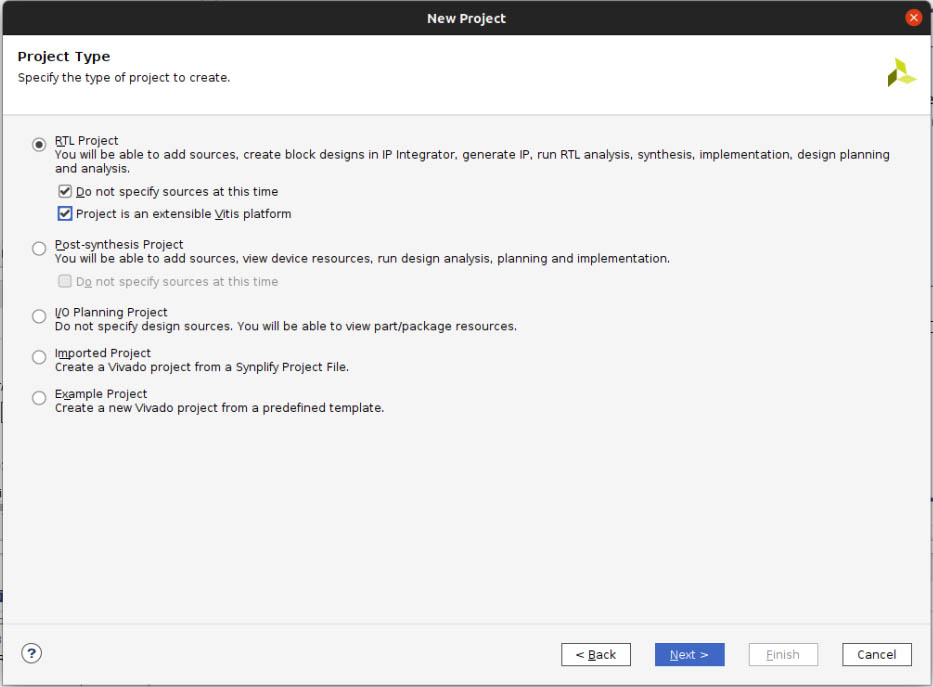
\includegraphics[width=0.65\textwidth]{src/png/kr26-xilinx-vivado-flow/kr26-xilix-vivado-flow-01.jpg}
					\caption{Xilinx Vivado – volba typu projektu, použitelného dále jako platforma ve Vitis, pro Xilinx KR26.}
					\label{fig:kr26-xilix-vivado-flow-01}
				\end{figure}

				Dalším krokem při zakládání projektu je zvolení prvku, na který bude vyvíjený HW design určen. Je možné zvolit přímo komponentu, pro kterou je design určen nebo již přednastavené vývojové desky. Pokud není vývojová deska v repozitáři od Xilinx, je možné jí vložit dle způsobu popsaného v části \hyperref[subsec:vivado-board-files]{\textit{Vivado Board Files}}. Xilinx Kria KR260 je však již součástí daného repozitáře a je možné ji v repozitáři vyhledat a zvolit. Výběr desky z repozitáře je zobrazen na obr. \ref{fig:kr26-xilix-vivado-flow-02}.

				\begin{figure}[htbp!]
					\centering
					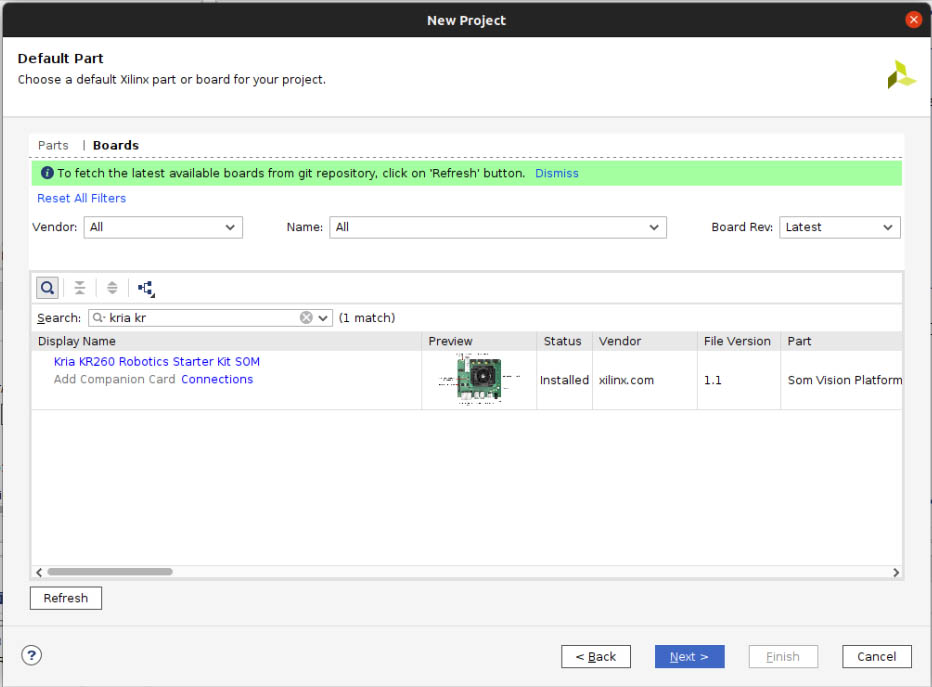
\includegraphics[width=0.75\textwidth]{src/png/kr26-xilinx-vivado-flow/kr26-xilix-vivado-flow-02.jpg}
					\caption{Xilinx Vivado – výběr základní komponenty, pro který bude HW design vytvářen.}
					\label{fig:kr26-xilix-vivado-flow-02}
				\end{figure}

				Po vytvoření projektu je uživateli zobrazena hlavní Vivado obrazovka. V základním nastavení jsou v pravé části obrazovky zobrazeny informace o vybrané základní komponentě/desce a v levé části pracovní menu. Pro pokračování ve vytváření designu je třeba zvolit v menu odkaz \textit{Create block design} a pojmenovat jej dle požadavků autora designu. Zvýrazněné menu a nabídka vytváření blokového je zobrazena na obr. \ref{fig:kr26-xilix-vivado-flow-03}.
		
				\begin{figure}[htbp!]
					\centering
					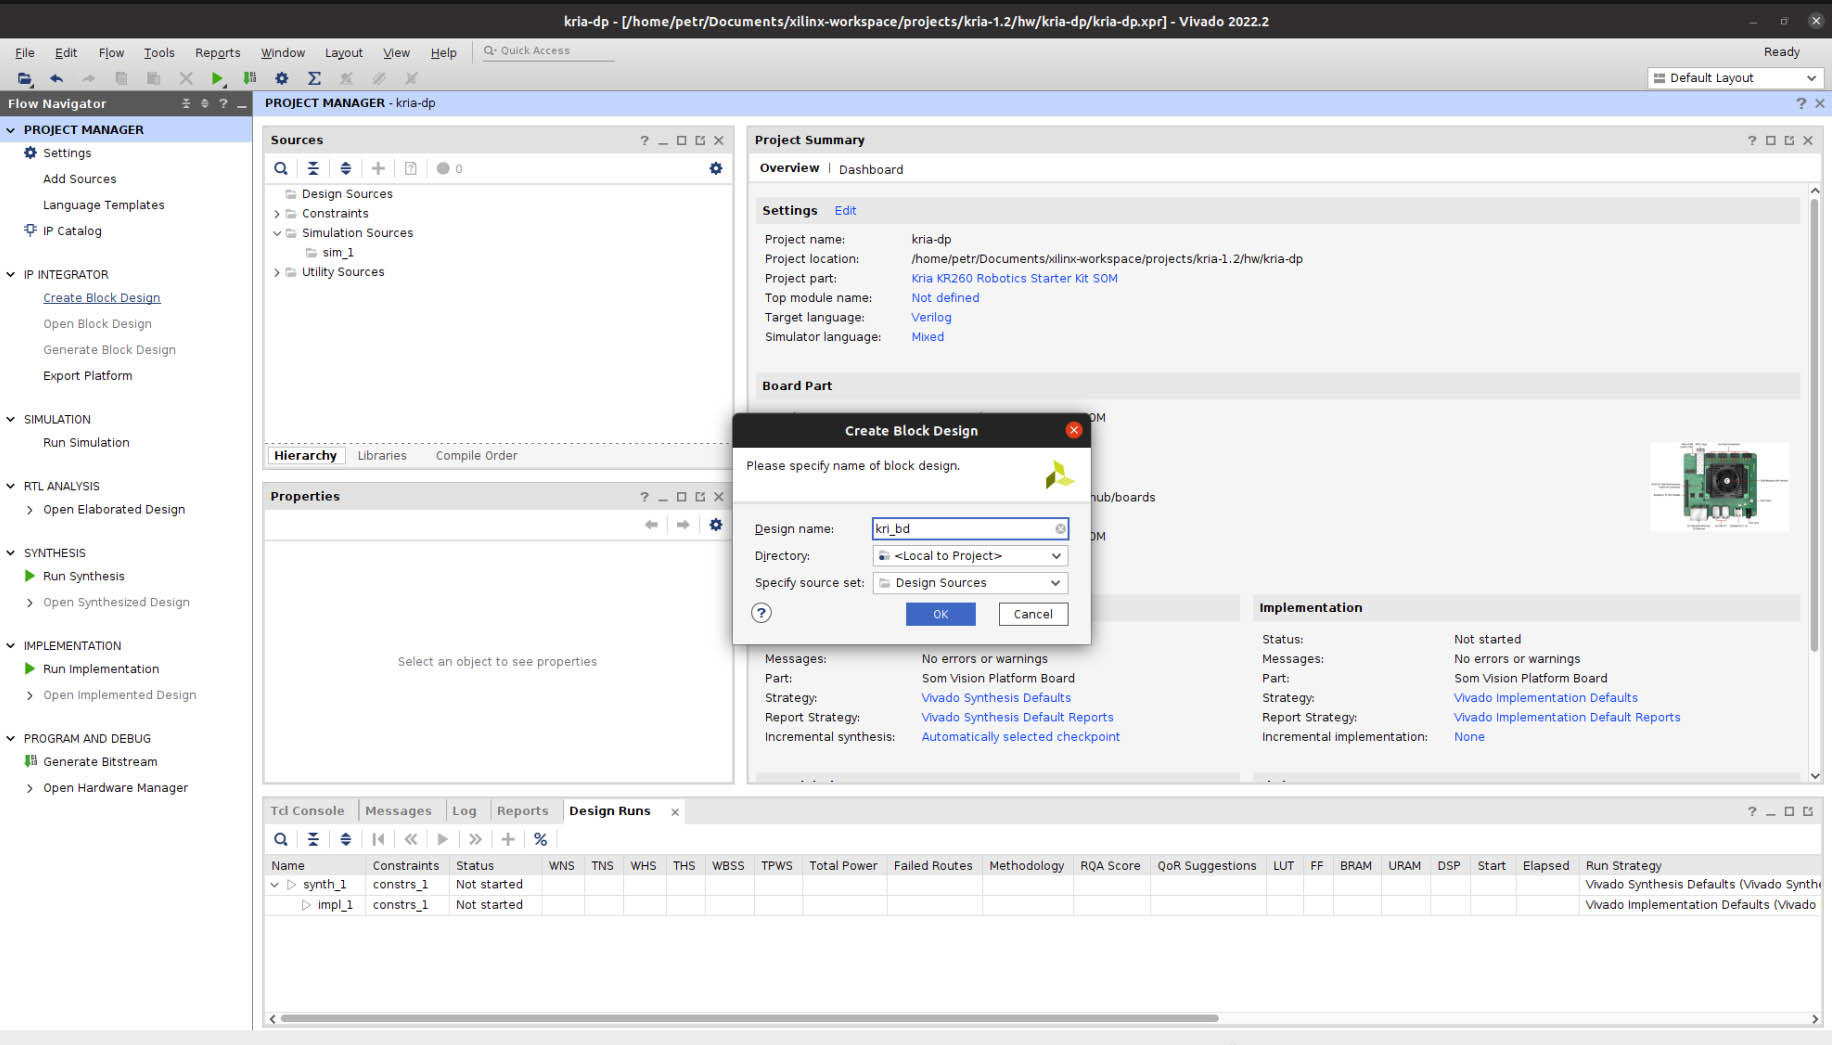
\includegraphics[width=0.75\textwidth]{src/png/kr26-xilinx-vivado-flow/kr26-xilix-vivado-flow-03.jpg}
					\caption{Xilinx Vivado – nabídka vytváření block design.}
					\label{fig:kr26-xilix-vivado-flow-03}
				\end{figure}

				Až po krok vytváření block designu byl postup velmi podobný pro obě představené vývojové desky. Nyní je již možné přistoupit k vlastní tvorbě blokového designu v kartě \textit{Diagram}.\par
				Bloky lze přidávat znakem \texttt{+} v aktivním okně nebo po kliknutím pravého tlačítka myši do volného prostoru v téže okně a zvolení \textit{Add IP} (IP – Intellectual Property). Prvním krokem je přidání PS, v případě Xilinx KR26 se jedná o IP y názvem \texttt{Zynq UltraScale+ MPSoC}. Výhoda používání Vivado je taková, že po vložení některých bloků je k dispozici aktivace automatického propojení/nastavení vybraných bloků IP. Po vložení PS bloku je vhodné tuto automatizaci spustit pomocí aktivního odkazu, zobrazeného na kartě \textit{Diagram} v obr. \ref{fig:kr26-xilix-vivado-flow-05}.

				\begin{figure}[htbp!]
					\centering
					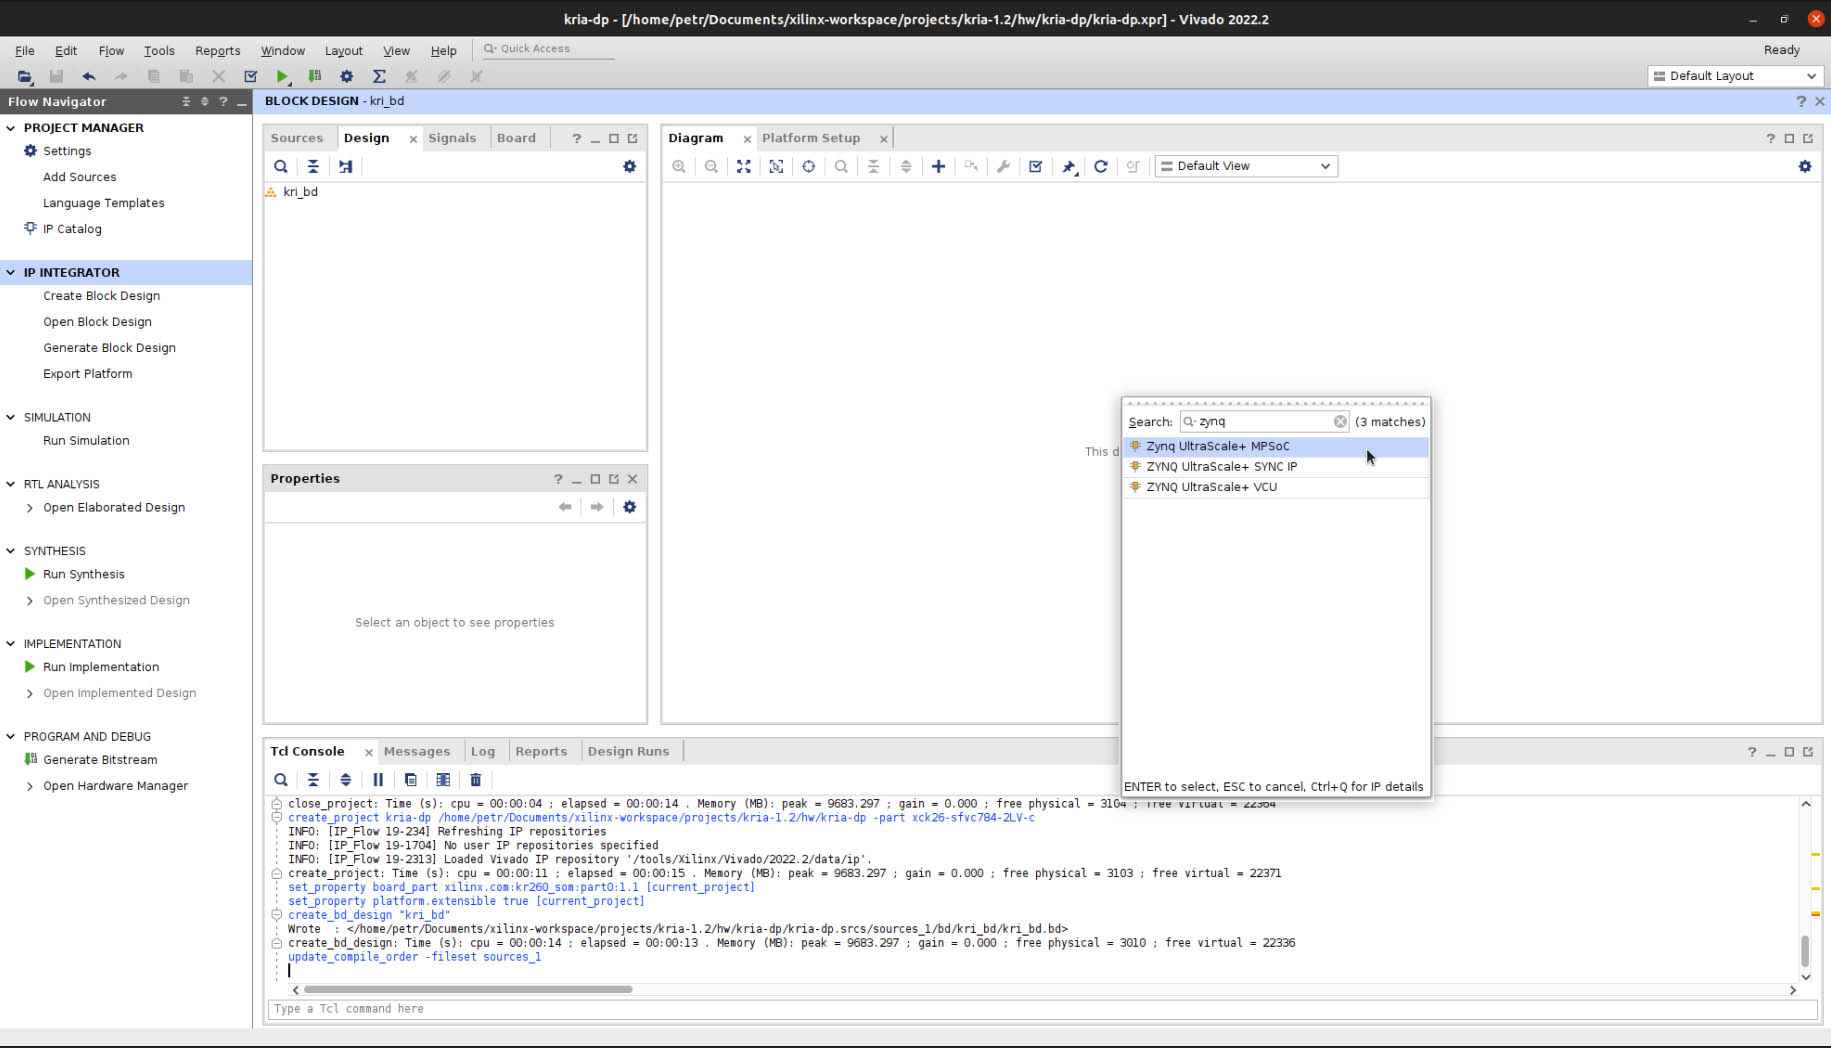
\includegraphics[width=0.75\textwidth]{src/png/kr26-xilinx-vivado-flow/kr26-xilix-vivado-flow-04.jpg}
					\caption{Xilinx Vivado – vložení PS IP bloku.}
					\label{fig:kr26-xilix-vivado-flow-04}
				\end{figure}

				\begin{figure}[htbp!]
					\centering
					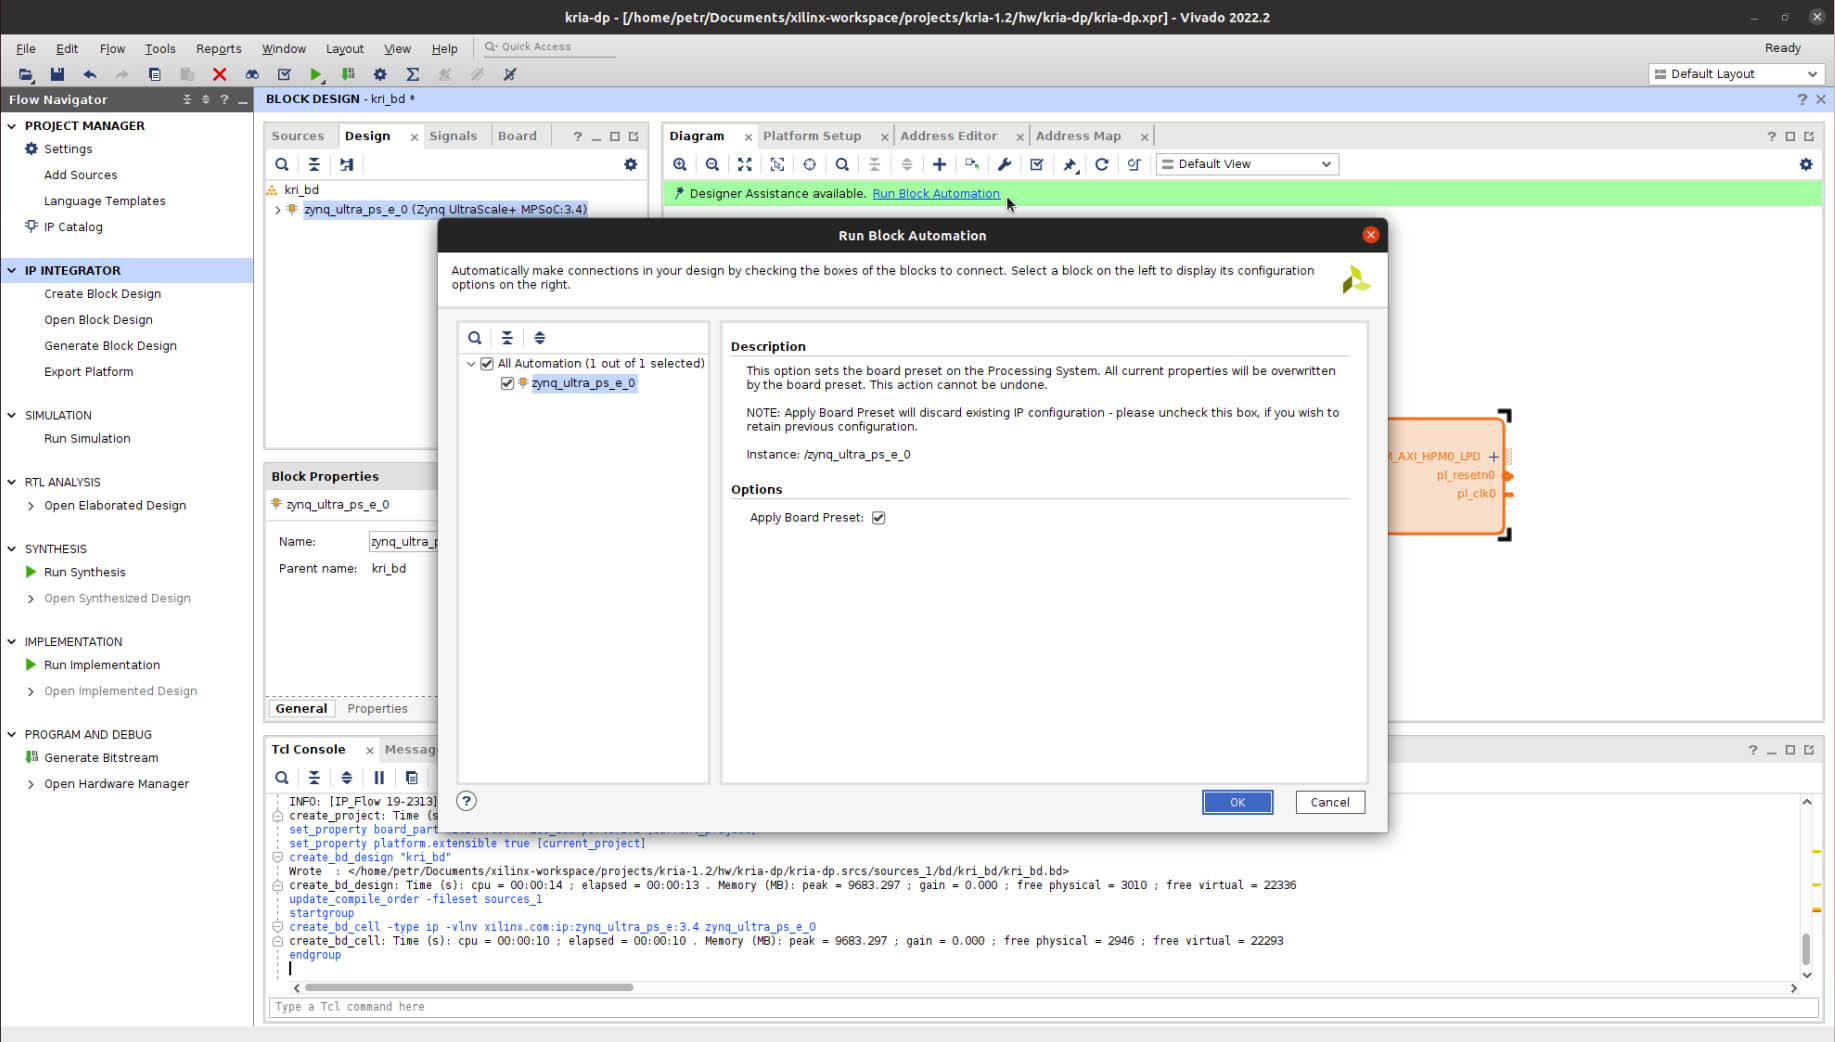
\includegraphics[width=0.75\textwidth]{src/png/kr26-xilinx-vivado-flow/kr26-xilix-vivado-flow-05.jpg}
					\caption{Xilinx Vivado – automatické propojení pro PS.}
					\label{fig:kr26-xilix-vivado-flow-05}
				\end{figure}

				Další krok je důležitý pro tvorbu akcelerované aplikace pomocí Vitis. Je třeba předkonfigurovat PS AXI Interface (rozhraní) takovým způsobem, aby AXI Interface s vysokým výkonem bylo využito až pro akcelerovanou aplikaci a nikoliv v některém z automatických propojení, jejichž pozitivní přínos byl představen v předchozím odstavci. Tato informace je popsána jak v \cite{hackster-getting-started-with-the-kria-kr260-in-vivado} ale také v oficiálních příkladových \cite{xilinx-github-vitis-tutorials-step-1-create-the-vivado-hardware-design-and-generate-xsa} (\textit{v sekci Add Interrupt Support, krok 1}) pro tvorbu platformy pro vývojovou desku Xilinx Kria KV260, jež používá totožný modul Xilinx Kria K26. Obr. \ref{fig:kr26-xilix-vivado-flow-06} obsahuje snímek obrazovky s požadovaným nastavením bloku \texttt{Zynq UltraScale+ MPSoC} a daných rozhraní.

				\begin{figure}[htbp!]
					\centering
					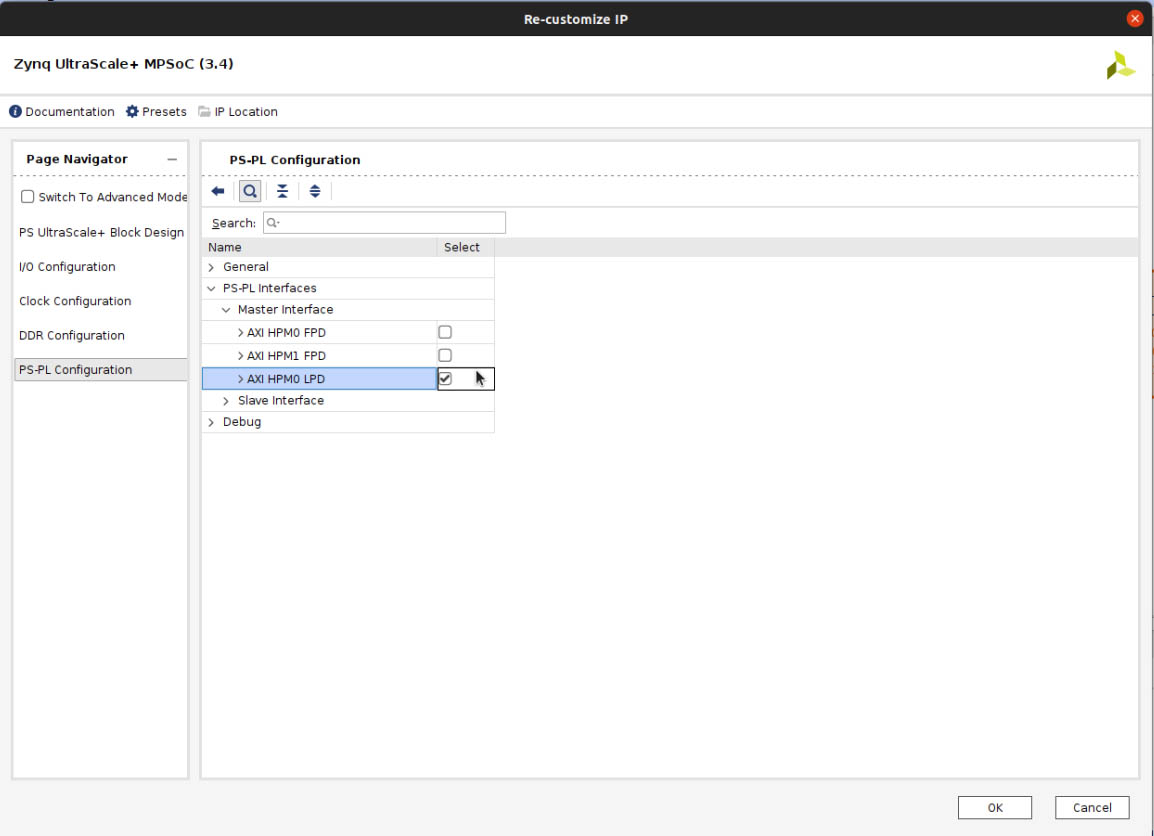
\includegraphics[width=0.75\textwidth]{src/png/kr26-xilinx-vivado-flow/kr26-xilix-vivado-flow-06.jpg}
					\caption{Xilinx Vivado – zablokování FPD a odblokování LPD pro block design.}
					\label{fig:kr26-xilix-vivado-flow-06}
				\end{figure}

				Protože dle \cite{xilinx-github-vitis-tutorials-step-1-create-the-vivado-hardware-design-and-generate-xsa} je počet clock signálů \texttt{pl\_clk} z PS omezený, je vhodné pro vytvoření požadovaných taktovacích signálů využít blok \texttt{Clocking wizard}. V tomto bloku je možné vytvořit taktovací signály s požadovanými parametry. Pokud počet signálů nestačí, je možné přidat další IP.\par
				Pro design ukázkové platformy v této práci je vhodné přidat tři taktovací signály s frekvencí 100, 200 a 20 MHz. také je důležité nastavit \textit{Reset type} na \textit{Active Low}. Příklad nastavení bloku \texttt{Clocking wizard} je na obr. \ref{fig:kr26-xilix-vivado-flow-07}.

				\begin{figure}[htbp!]
					\centering
					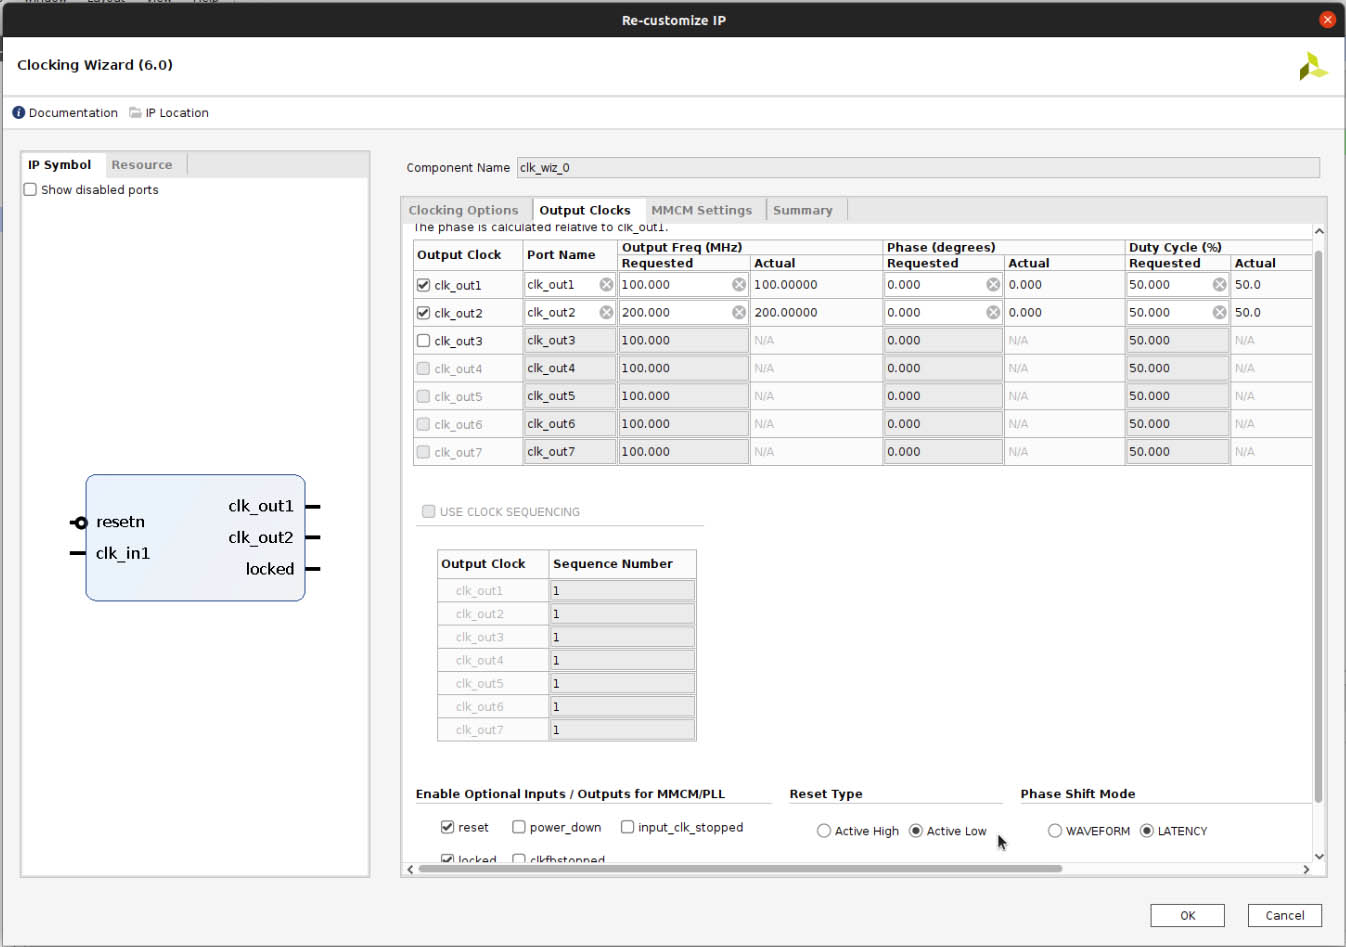
\includegraphics[width=0.75\textwidth]{src/png/kr26-xilinx-vivado-flow/kr26-xilix-vivado-flow-07.jpg}
					\caption{Xilinx Vivado – nastavení bloku Clocking wizard.}
					\label{fig:kr26-xilix-vivado-flow-07}
				\end{figure}
				Po nastavení požadovaných taktovacích signálů je možné opět pomocí aktivního odkazu automatizace spustit automatické propojení bloků. Po úspěšném provedení předchozích konfiguračních kroků a automatizace je získáno schéma blokového designu na obr. \ref{fig:kr26-xilix-vivado-flow-08}.

				\begin{figure}[htbp!]
					\centering
					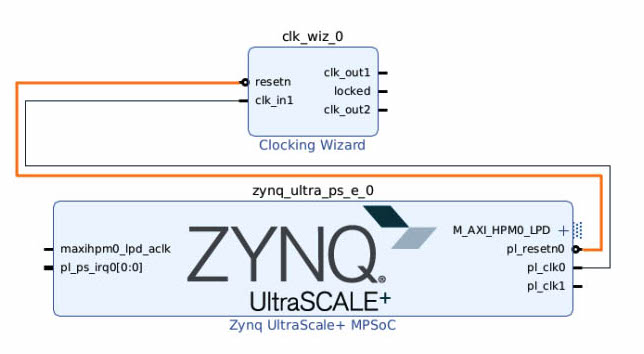
\includegraphics[width=0.75\textwidth]{src/png/kr26-xilinx-vivado-flow/kr26-xilix-vivado-flow-08.jpg}
					\caption{Xilinx Vivado – blokový design s PS a blokem Clocking wizard po provedení automatizace.}
					\label{fig:kr26-xilix-vivado-flow-08}
				\end{figure}

				K bloku \texttt{Clocking Wizard} je nyní vhodné připojit bloky \texttt{Processor System Reset} dle obr. \ref{fig:kr26-xilix-vivado-flow-09}.

				\begin{figure}[htbp!]
					\centering
					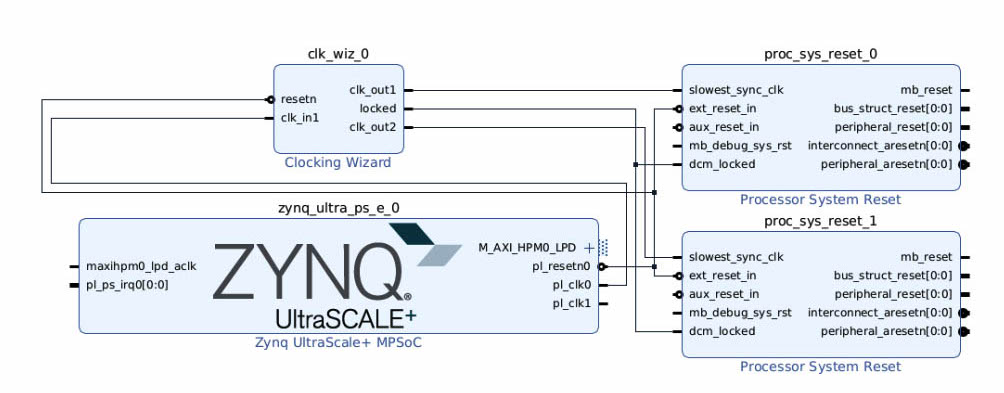
\includegraphics[width=0.95\textwidth]{src/png/kr26-xilinx-vivado-flow/kr26-xilix-vivado-flow-09.jpg}
					\caption{Xilinx Vivado – propojení bloků Clocking wizard a Processor System Reset.}
					\label{fig:kr26-xilix-vivado-flow-09}
				\end{figure}
				
				Vstup pro přerušení \texttt{pl\_ps irq} může obsahovat maximálně 16 interrupt signálů. Pro design v této aplikaci to je dostačující případ, ovšem pokud je vyžadováno, aby aplikace využívala více signálů přerušení, je třeba využít blok \texttt{AXI Interrupt Controller}. Doporučené nastavení tohoto IP je na obr. \ref{fig:kr26-xilix-vivado-flow-10}. Aby bylo možné připojit signál k \texttt{pl\_ps irq} je nutné přepnout nastavení \textit{Processor Interrupt Type and Connection -> Interrupt Output Connection} na \texttt{Single} z výchozího \texttt{Bus}.\par
				V případě nevyužití bloku \texttt{AXI Interrupt Controller}, nebo při snaze přivést signály přerušení přímo do \texttt{pl\_ps irq} vstupu PS systému je pro připojení více signálů doporučeno použít IP blok \texttt{Concat}. V pokročilejší části této práci je tento blok také využit, aby byla demonstrována možnost jeho využití a projevení tohoto připojení v PetaLinux systému.\par
				Po dokončení konfigurace \texttt{AXI Interrupt Controller} je opět možné aktivovat automatizaci propojení a v konfiguračním okně vybrat požadovanou frekvenci clock signálů. V této práci je využito 200 MHz. Výsledný design po automatizaci je zobrazen na obr. \ref{fig:kr26-xilix-vivado-flow-12}.\par

				\begin{figure}[htbp!]
					\centering
					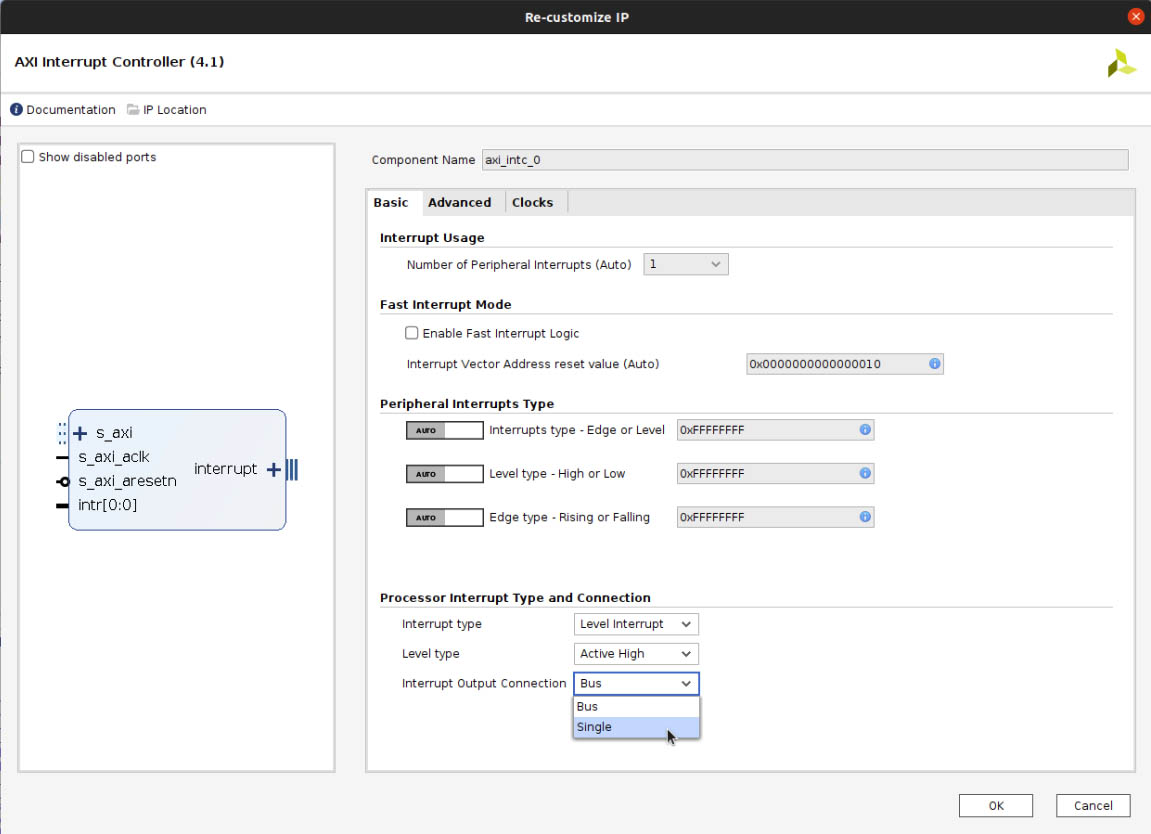
\includegraphics[width=0.75\textwidth]{src/png/kr26-xilinx-vivado-flow/kr26-xilix-vivado-flow-10.jpg}
					\caption{Xilinx Vivado – nastavení bloku AXI Interrupt Controller.}
					\label{fig:kr26-xilix-vivado-flow-10}
				\end{figure}

				\begin{figure}[htbp!]
					\centering
					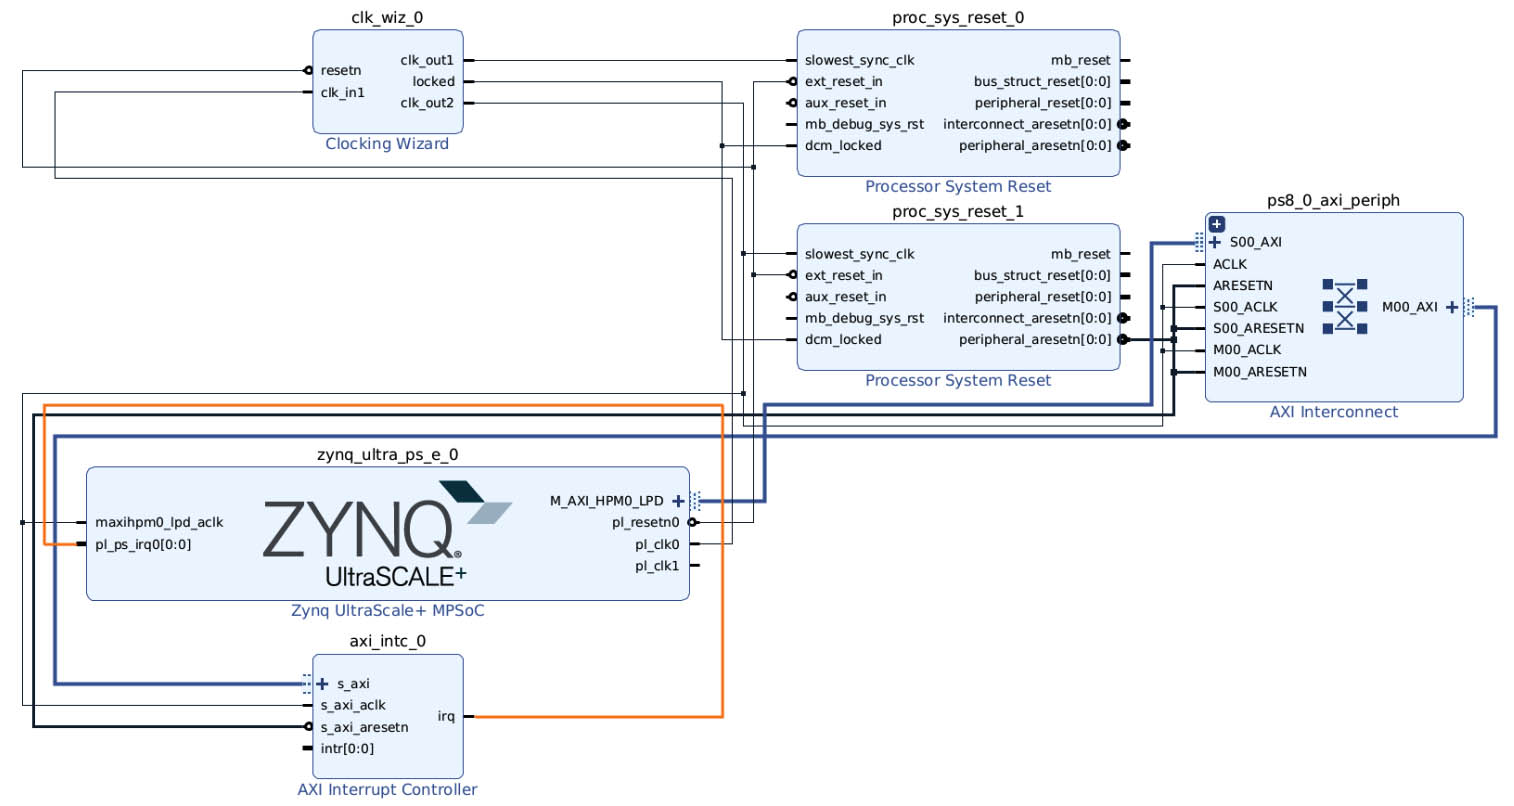
\includegraphics[width=0.95\textwidth]{src/png/kr26-xilinx-vivado-flow/kr26-xilix-vivado-flow-12.jpg}
					\caption{Xilinx Vivado – block design po automatizaci a propojení bloku AXI Interrupt Controller.}
					\label{fig:kr26-xilix-vivado-flow-12}
				\end{figure}

				Pokud by vyvíjená aplikace nevyužívala další PL IP bloky, je možné přistoupit ke konfiguraci platformy, PS a periferií připojených k PS. Pro vyvíjenou ukázkovou aplikaci je vytvořený HW blokový design naznačen v sekci \hyperref[subsubsec:hw-block-design-vyvijene-aplikace]{\textit{HW Block design vyvíjené aplikace}}.\par
				Na kartě \textit{Platform Setup} je pro funkční design vhodné aktivovat a pojmenovat základní AXI porty dle tabulky \ref{tab:vivado-platform-setup-axi-xilinx-kria}.


				\begin{table}[H]
					\centering
					\caption{Ukázka nastavených AXI portů v~Xilinx Vivado platformě pro \textit{Xilinx Kria KR260}.}
				  \vspace*{0.15cm}
				
					\begin{tabular}{!{\vrule width 2pt} c | c | c | c !{\vrule width 2pt}}
					\noalign{\hrule height 2pt}
					Name & Enabled & Memport & SP Tag\\
					\noalign{\hrule height 2pt}
					M\_AXI\_HPM0\_FPD & X & M\_AXI\_GP & -\\ \hline
					M\_AXI\_HPM1\_FPD & X & M\_AXI\_GP & -\\ \hline
					S\_AXI\_HPC0\_FPD & X & S\_AXI\_HPC & HPC0\\ \hline
					S\_AXI\_HPC1\_FPD & X & S\_AXI\_HPC & HPC1\\ \hline
					S\_AXI\_HP0\_FPD & X & S\_AXI\_HP & HP0\\ \hline
					S\_AXI\_HP1\_FPD & X & S\_AXI\_HP & HP1\\ \hline
					S\_AXI\_HP2\_FPD & X & S\_AXI\_HP & HP2\\ \hline
					S\_AXI\_HP3\_FPD & X & S\_AXI\_HP & HP3\\ \noalign{\hrule height 2pt}
					\end{tabular}
					\label{tab:vivado-platform-setup-axi-xilinx-kria}
				\end{table}


				
			\fbar
			\subsubsection{HW block design vyvíjené aplikace}\label{subsubsec:hw-block-design-vyvijene-aplikace}

			\begin{figure}[htbp!]
				\centering
				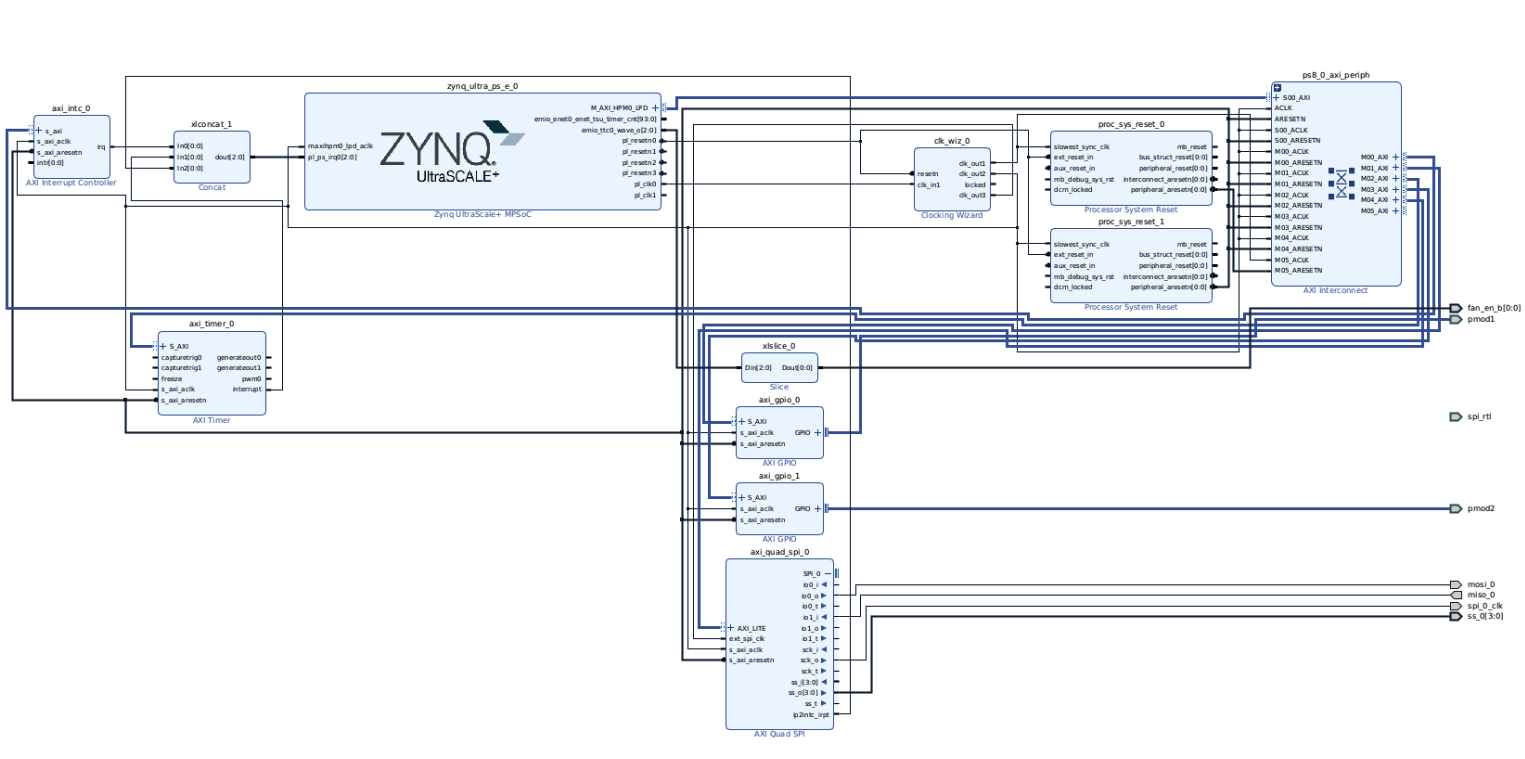
\includegraphics[width=0.95\textwidth]{src/png/kr-26-xilinx-vivado-hw-block-design.png}
				\caption{Xilinx Vivado – HW block design vyvíjené aplikace.}
				\label{fig:kr-26-xilinx-vivado-hw-block-design}
			\end{figure}

	% Basic popsání, možná si zjistit do hloubky co vše znamená
    % WorkFlow
    % Zjistit jak dát vstupem tlačítka a jak výstupy jako výstupy

	\fbar
	\subsection{Tvorba PetaLinux}\label{subsec:tvorba-petalinux}
	\subsection{Tvorba SW pro CPU a FPGA}
	\subsubsection{Upravený postup debuggingu PL pro Digilent Zybo}

	Debugging pro program pro PL. Pro host program je možné debuggovat přímo ve Vitis, ale bez PL kernelu.
	\begin{figure}[htbp!]
		\centering
		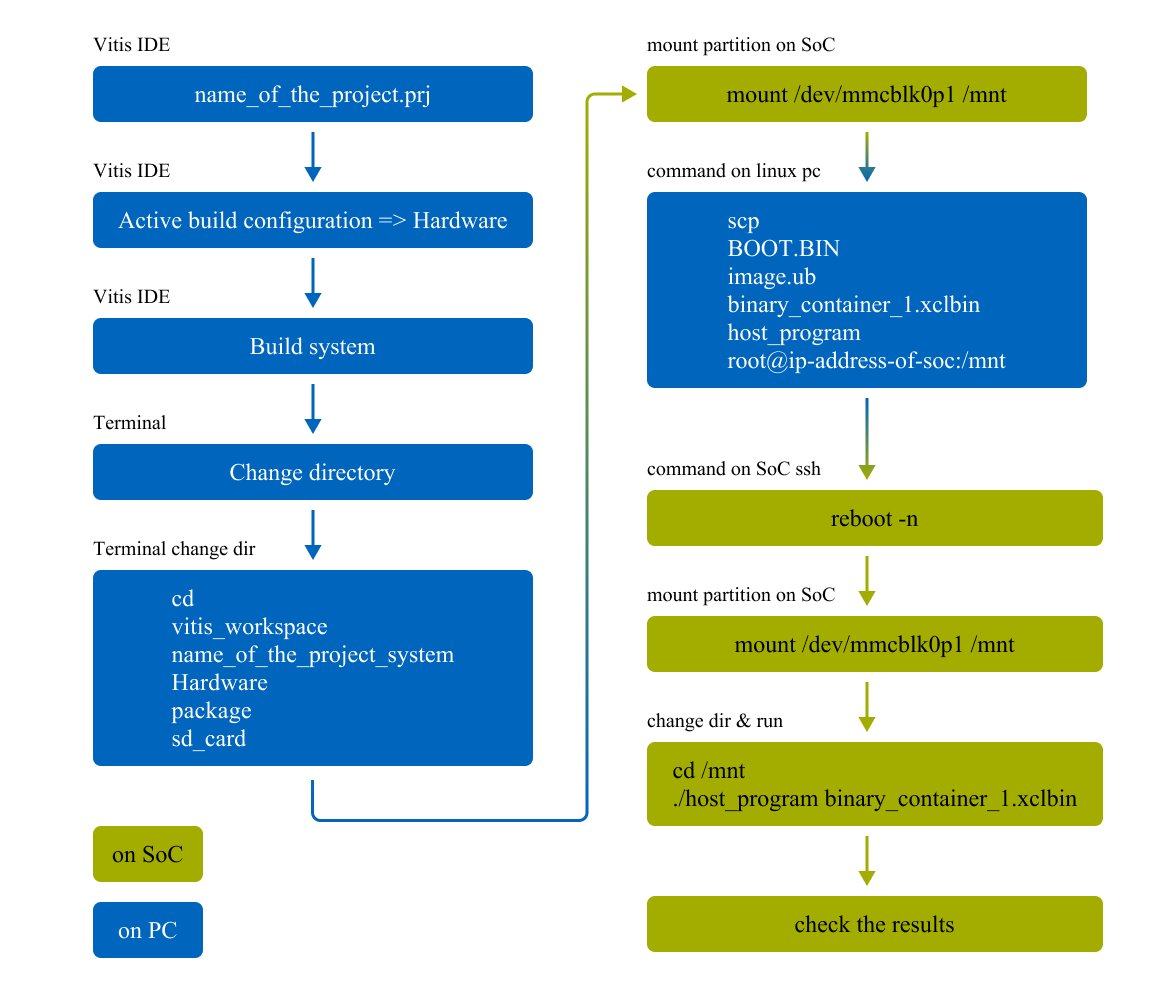
\includegraphics[width=0.85\textwidth]{src/png/vitis-edited-debugging-flow.png}
		\caption{Diagram popisující upravený postup pro debuggování a spouštění host programu a nahrávání host programu do PL}
		\label{fig:vitis-edited-debugging-flow}
	\end{figure}

\section{Představení pracoviště}
\section{Dosažené výsledky}


		
%závěr
\newpage
\addcontentsline{toc}{section}{\numberline{}Závěr} 
\section*{Závěr}
Aliquam dapibus leo velit, ultrices eleifend mi feugiat eget. Aliquam euismod facilisis turpis, nec lobortis libero aliquet sit amet. Aenean suscipit ante eget ipsum viverra hendrerit. Ut sed massa sed nisi tempus dapibus in eu enim. Nullam vitae odio laoreet, malesuada purus non, faucibus orci. Lorem ipsum dolor sit amet, consectetur adipiscing elit. Etiam eget odio quis enim laoreet imperdiet nec eu nunc. Maecenas ut consequat purus. Duis faucibus risus nec metus cursus placerat. Phasellus sapien justo, laoreet in pulvinar ut, maximus nec velit.\par
	

\flushbottom %vyčištění stránky

%konec závěru

\newpage
\setmonofont{Times New Roman}
\printbibliography[title={{Literatura}}]	
\nocite{*}
\setmonofont{Courier}
\addcontentsline{toc}{section}{\numberline{}Literatura} %Added citations to TOC%
	\appendix
	\titleformat{\section}{\color{ctublue}\fontspec{Times New Roman}\fontsize{15}{15}\bfseries}{Příloha \thesection:}{2.1em}{}
	\begin{appendices}
	\section{Seznam symbolů a zkratek}
		\subsection{Seznam symbolů}
			\begin{description}
			\item $\vec{F}$ (N) \hspace*{\parindent} vektor síly
		\end{description}
	\subsection{Seznam zkratek}
		\begin{description}
			\item DCM \hspace*{\parindent} DC Master
		\end{description}

		\section{Tvorba HW designu pro Digilent Zybo Zynq-7000 vývojovou desku}\label{sec:appendicies:-tvorba-hw-designu-pro-digilent-zybo-zynq-7000-vyvojovou-desku}
		V~této části bude představen postup tvorby HW architektury pro vývojovou desku Digilent Zybo Zynq-7000. Postup tvorby platformy byl částečně převzat z~\cite{hackster-vitis-2021-1-embedded-platform-for-zybo-z7-20}. V~případě, že je požadováno vytvoření dalších speciálních bloků v~čipu PL je třeba do blokového designu vložit odpovídající IP bloky, které zajistí potřebnou funkcionalitu.\par
		Nejprve je nutné vytvořit nový Vivado projekt a pojmenovat ho dle požadavků. Při výběru typu projektu je nutné zvolit možnost \textit{RTL Project} a aktivovat možnost \textit{Project is an extensible Vitis platform}. Tento úkon je naznačen na obr. \ref{fig:zybo-xilinx-vivado-flow-01}.

			\begin{figure}[htbp!]
				\centering
				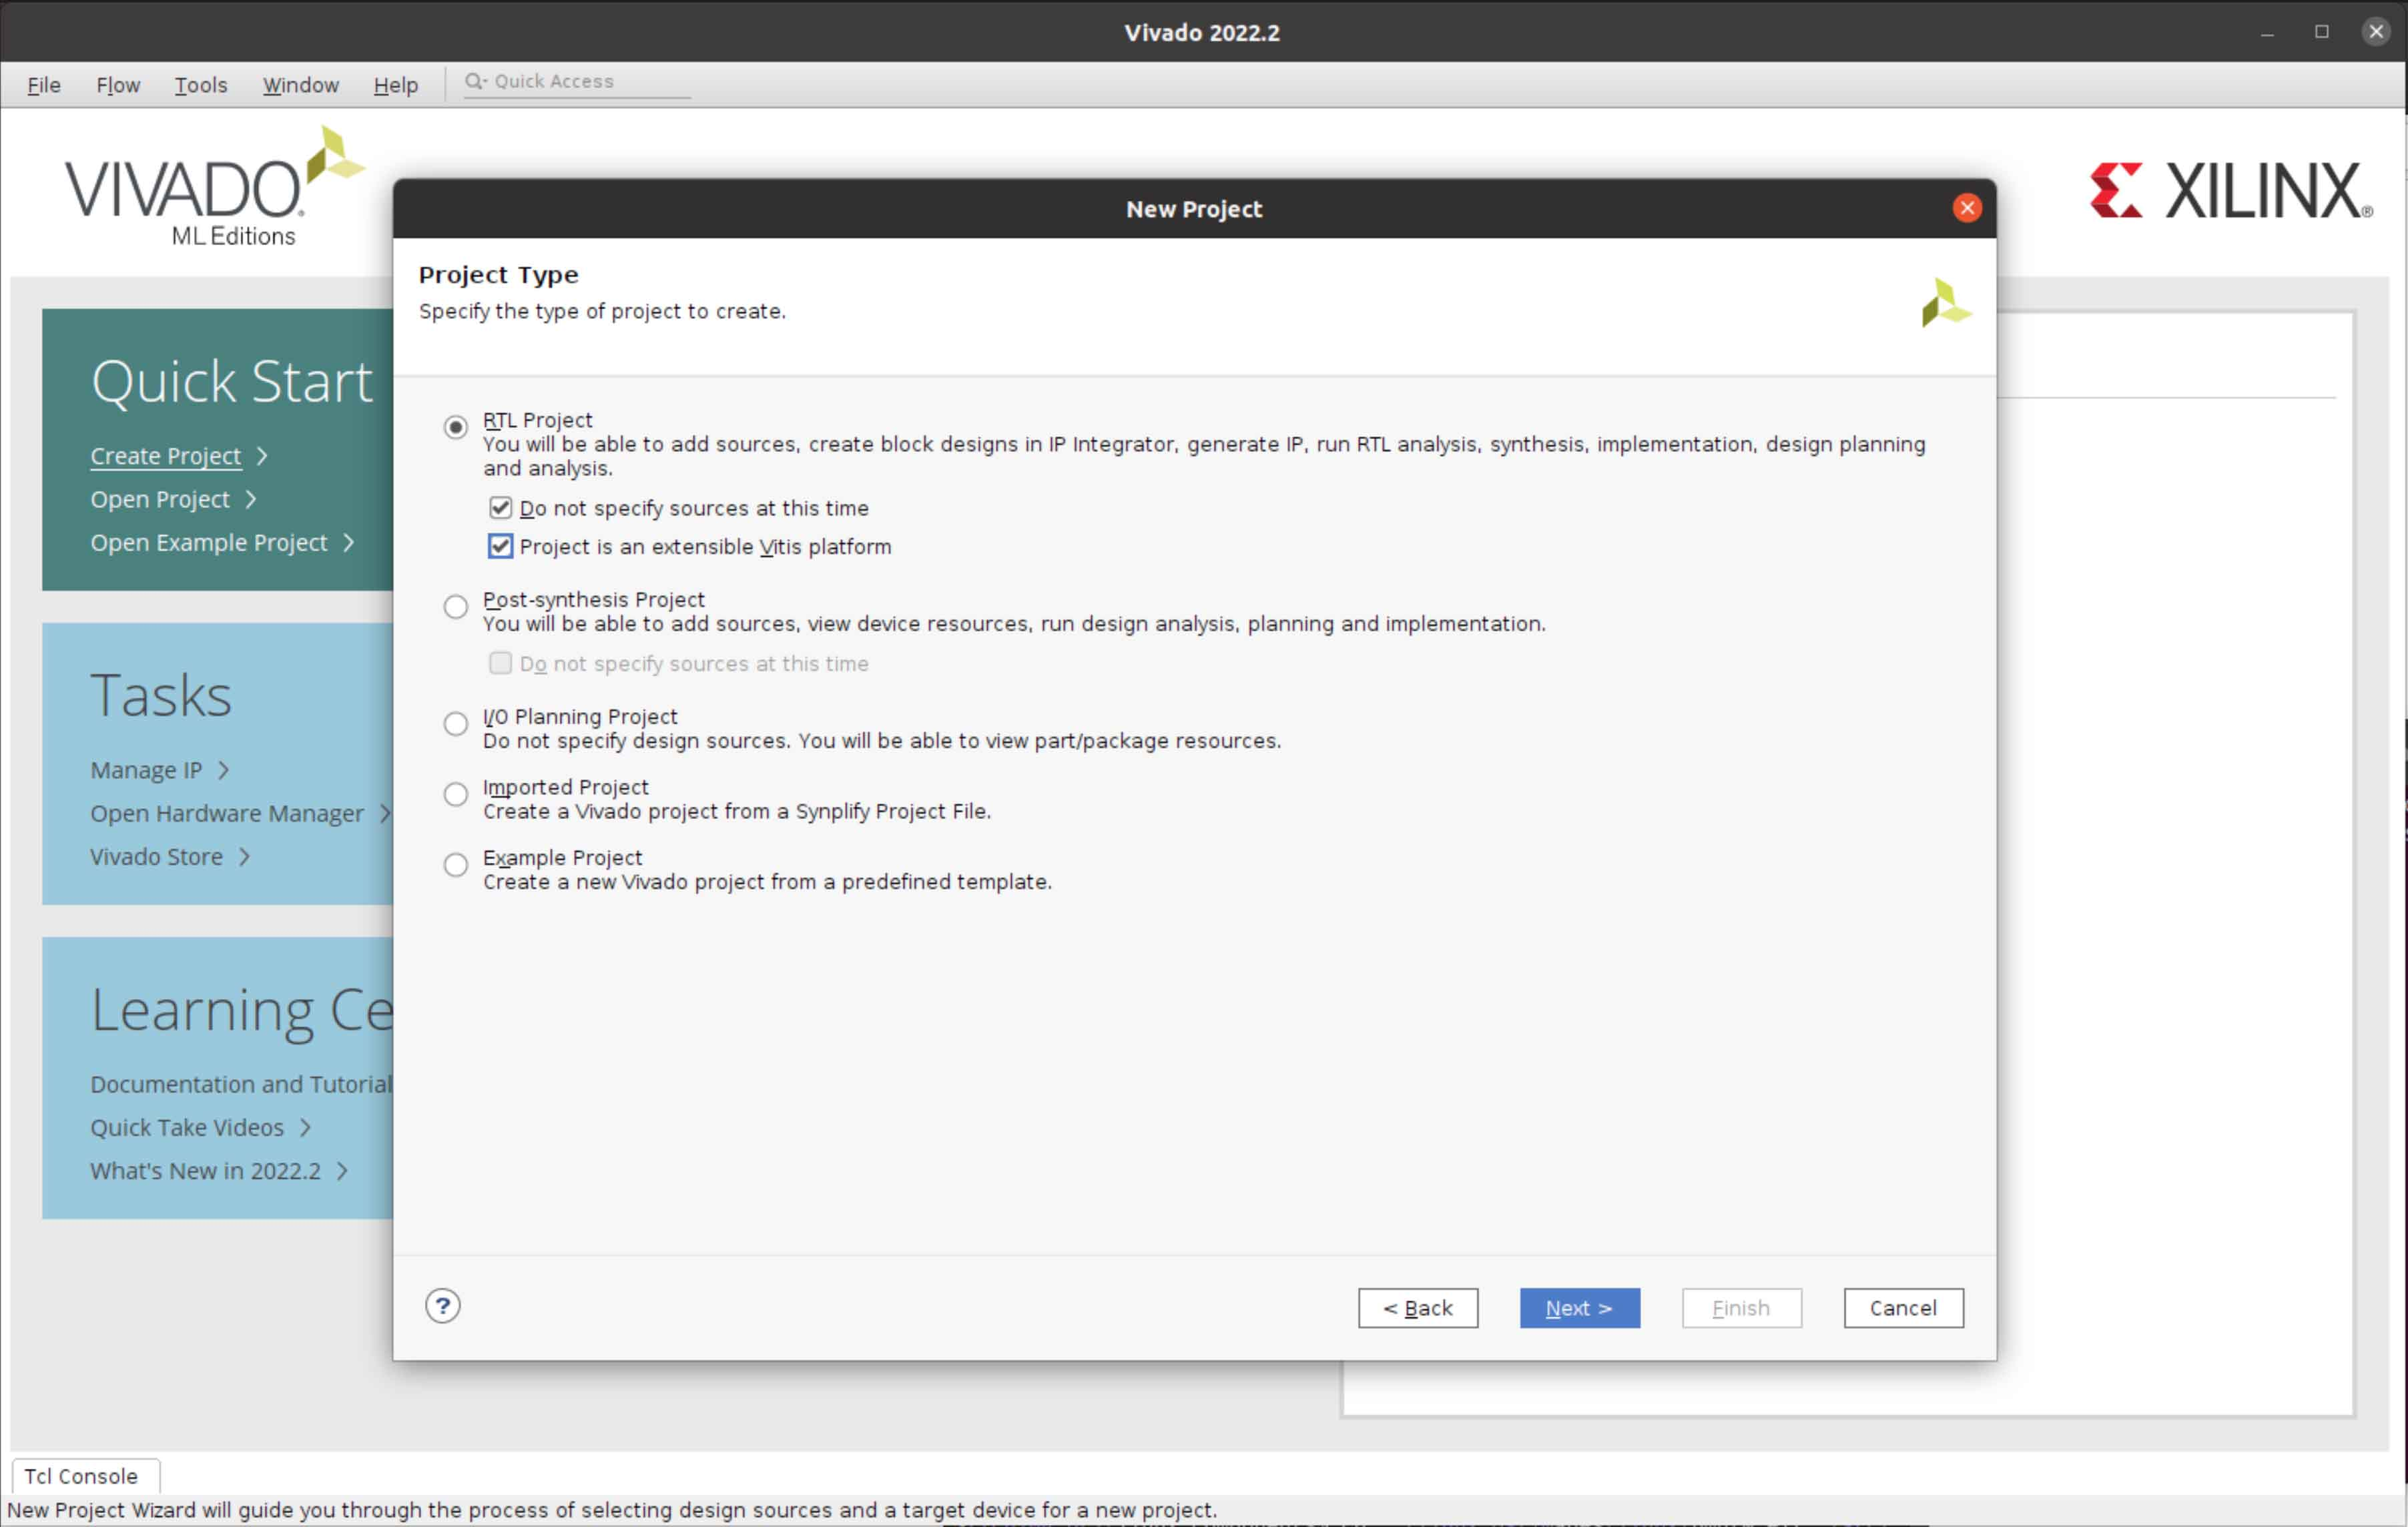
\includegraphics[width=0.75\textwidth]{src/png/zybo-xilinx-vivado-flow/zybo-xilinx-vivado-flow-01.jpg}
				\caption{Xilinx Vivado – volba typu projektu pro Digilent Zybo.}
				\label{fig:zybo-xilinx-vivado-flow-01}
			\end{figure}

		Následně v~nabídce \textit{Xilinx part} vybrat možnost \textit{Board} a do vyhledávání zadat název využívané desky. V~této práci bude využíváno desky \textit{Zybo}. Díky instalovaným \textit{board files}, představených v~části \hyperref[subsec:vivado-board-files]{\textit{Vivado Board Files}}, je možné nalézt požadovanou desku verze 2.0 a pokračovat v~tvorbě designu. Výběr základního HW je zobrazen na obr. \ref{fig:zybo-xilinx-vivado-flow-02}.

		\begin{figure}[htbp!]
			\centering
			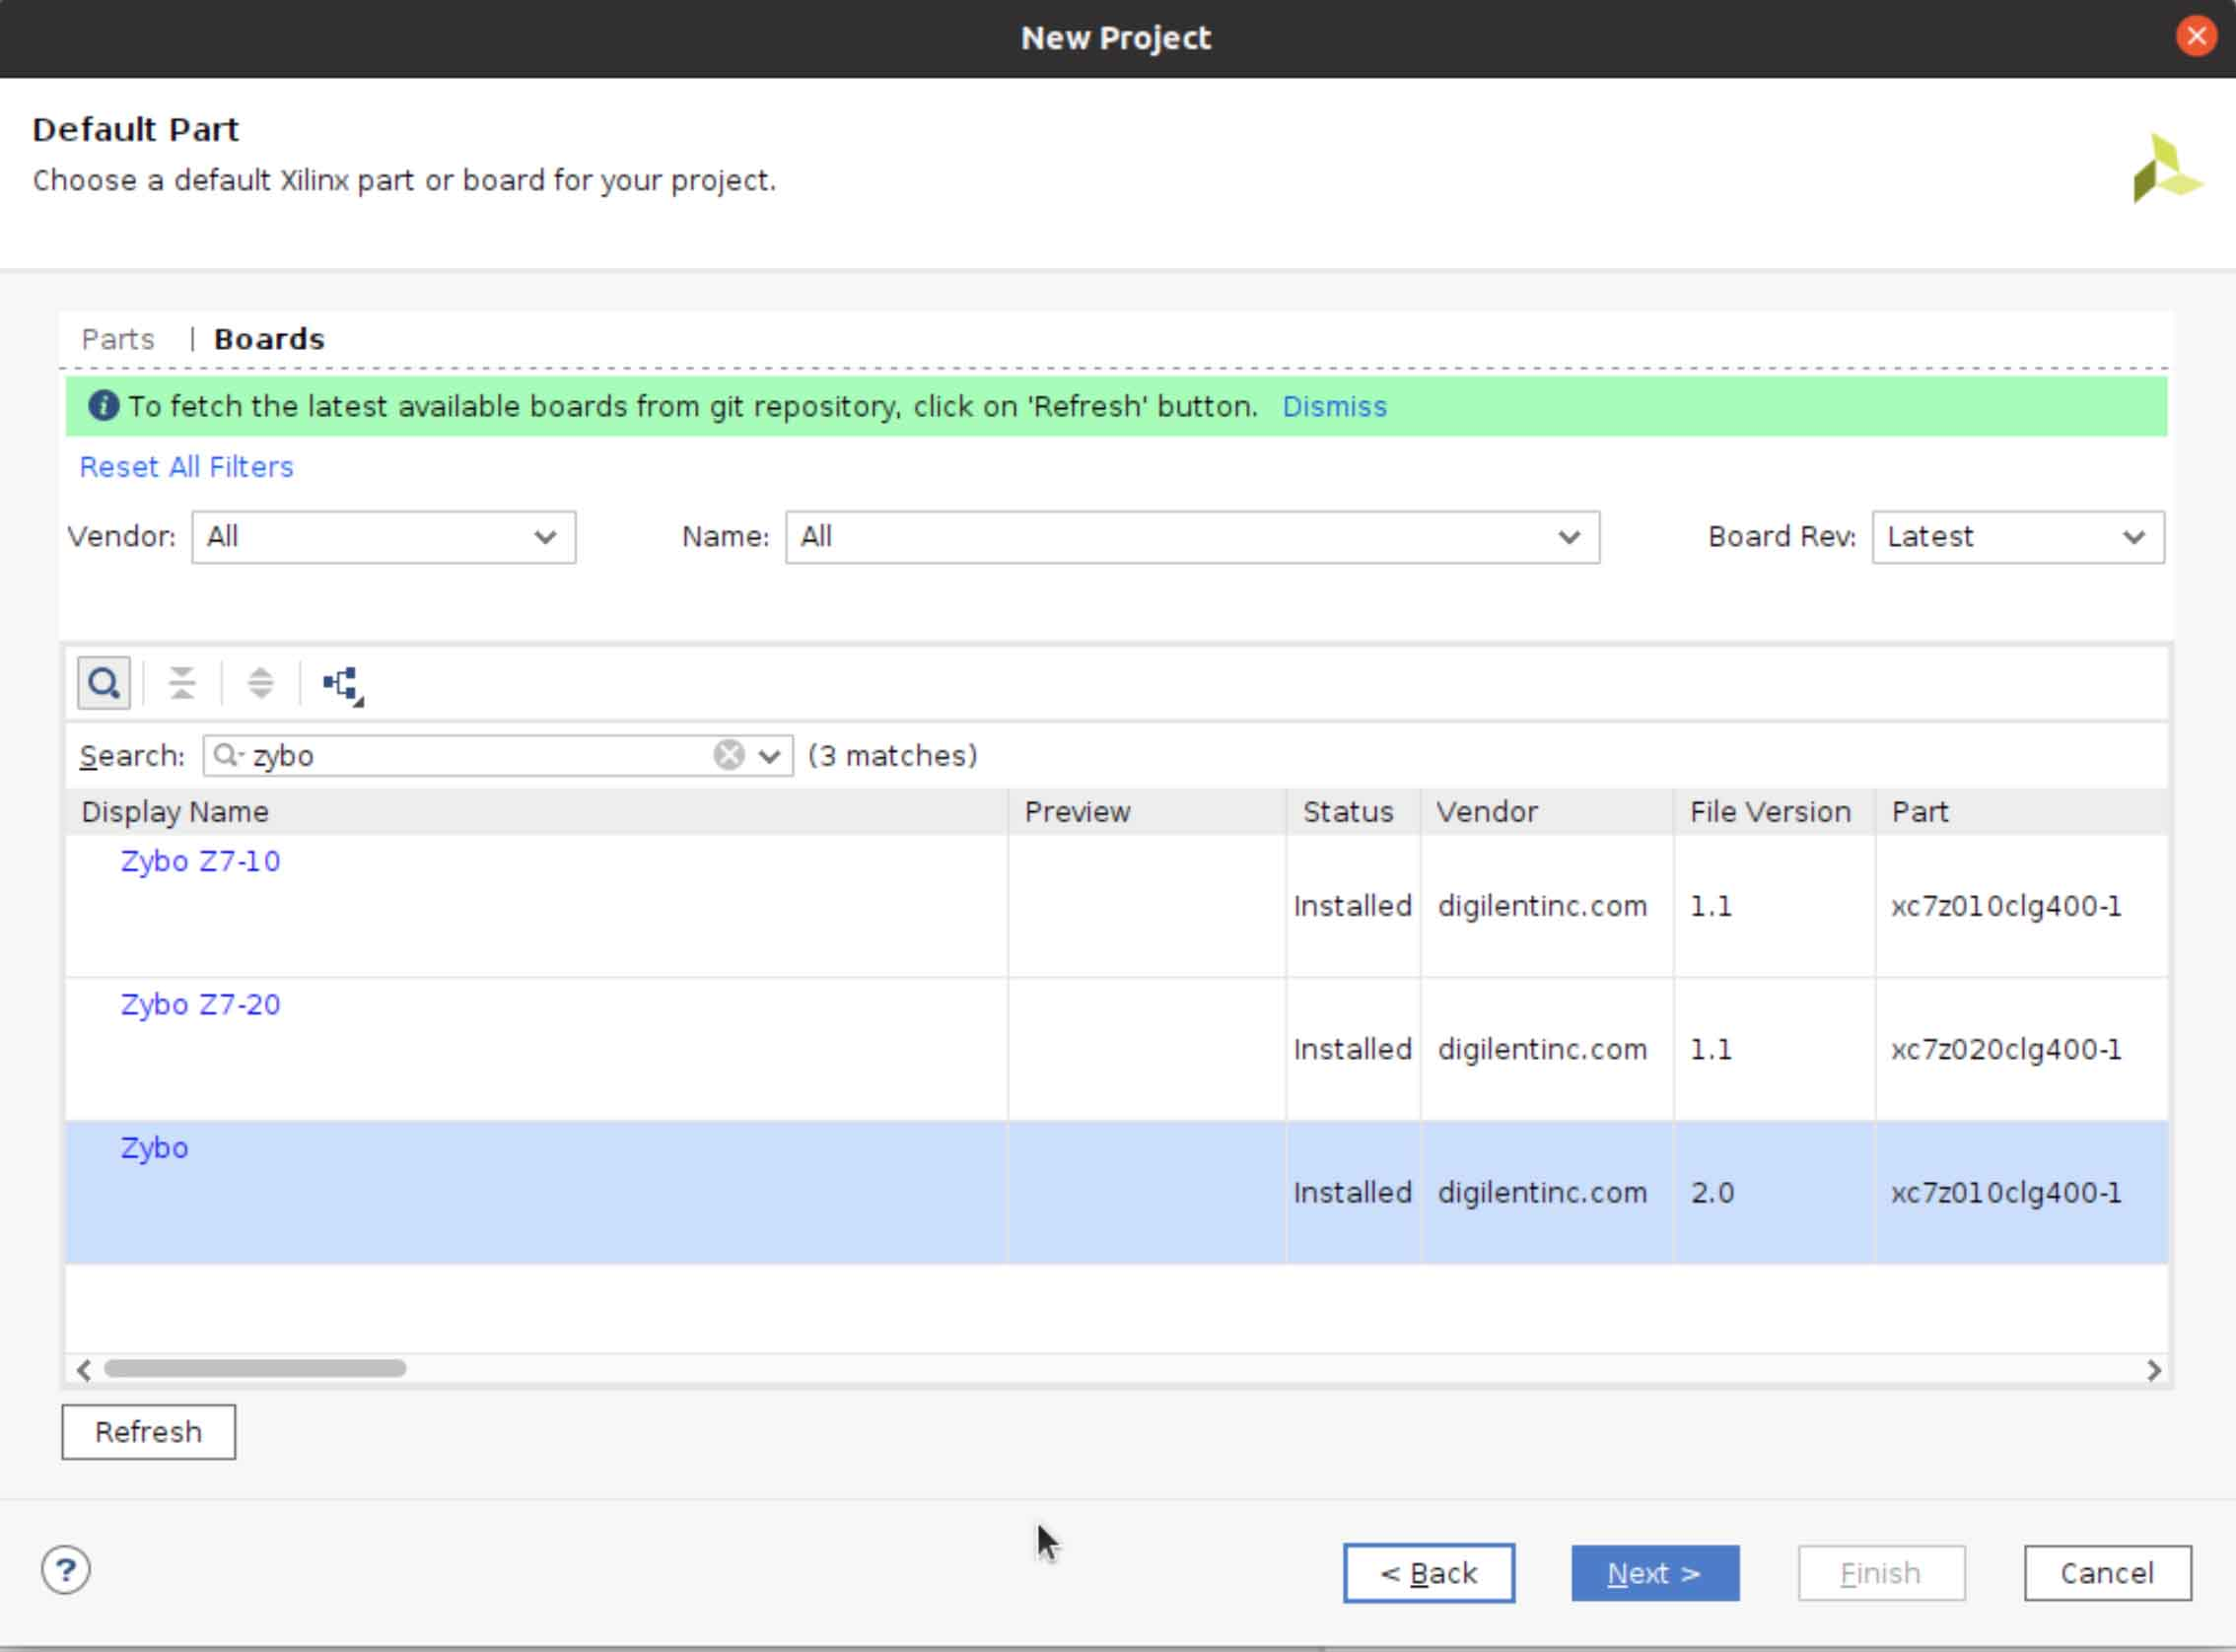
\includegraphics[width=0.75\textwidth]{src/png/zybo-xilinx-vivado-flow/zybo-xilinx-vivado-flow-02.jpg}
			\caption{Xilinx Vivado – výběr základního HW, pro který bude vytvářena architektura pro Digilent Zybo.}
			\label{fig:zybo-xilinx-vivado-flow-02}
		\end{figure}
		
		Po úspěšné inicializaci projektu je pro další pokračování nutné v~menu \textit{Flow Navigator/IP Integrator} zvolit možnost \textit{Create Block Design} a vytvořit nový blokový design. Tvorba blokového designu je naznačena na obr. \ref{fig:zybo-xilinx-vivado-flow-05}.
		
		\begin{figure}[htbp!]
			\centering
			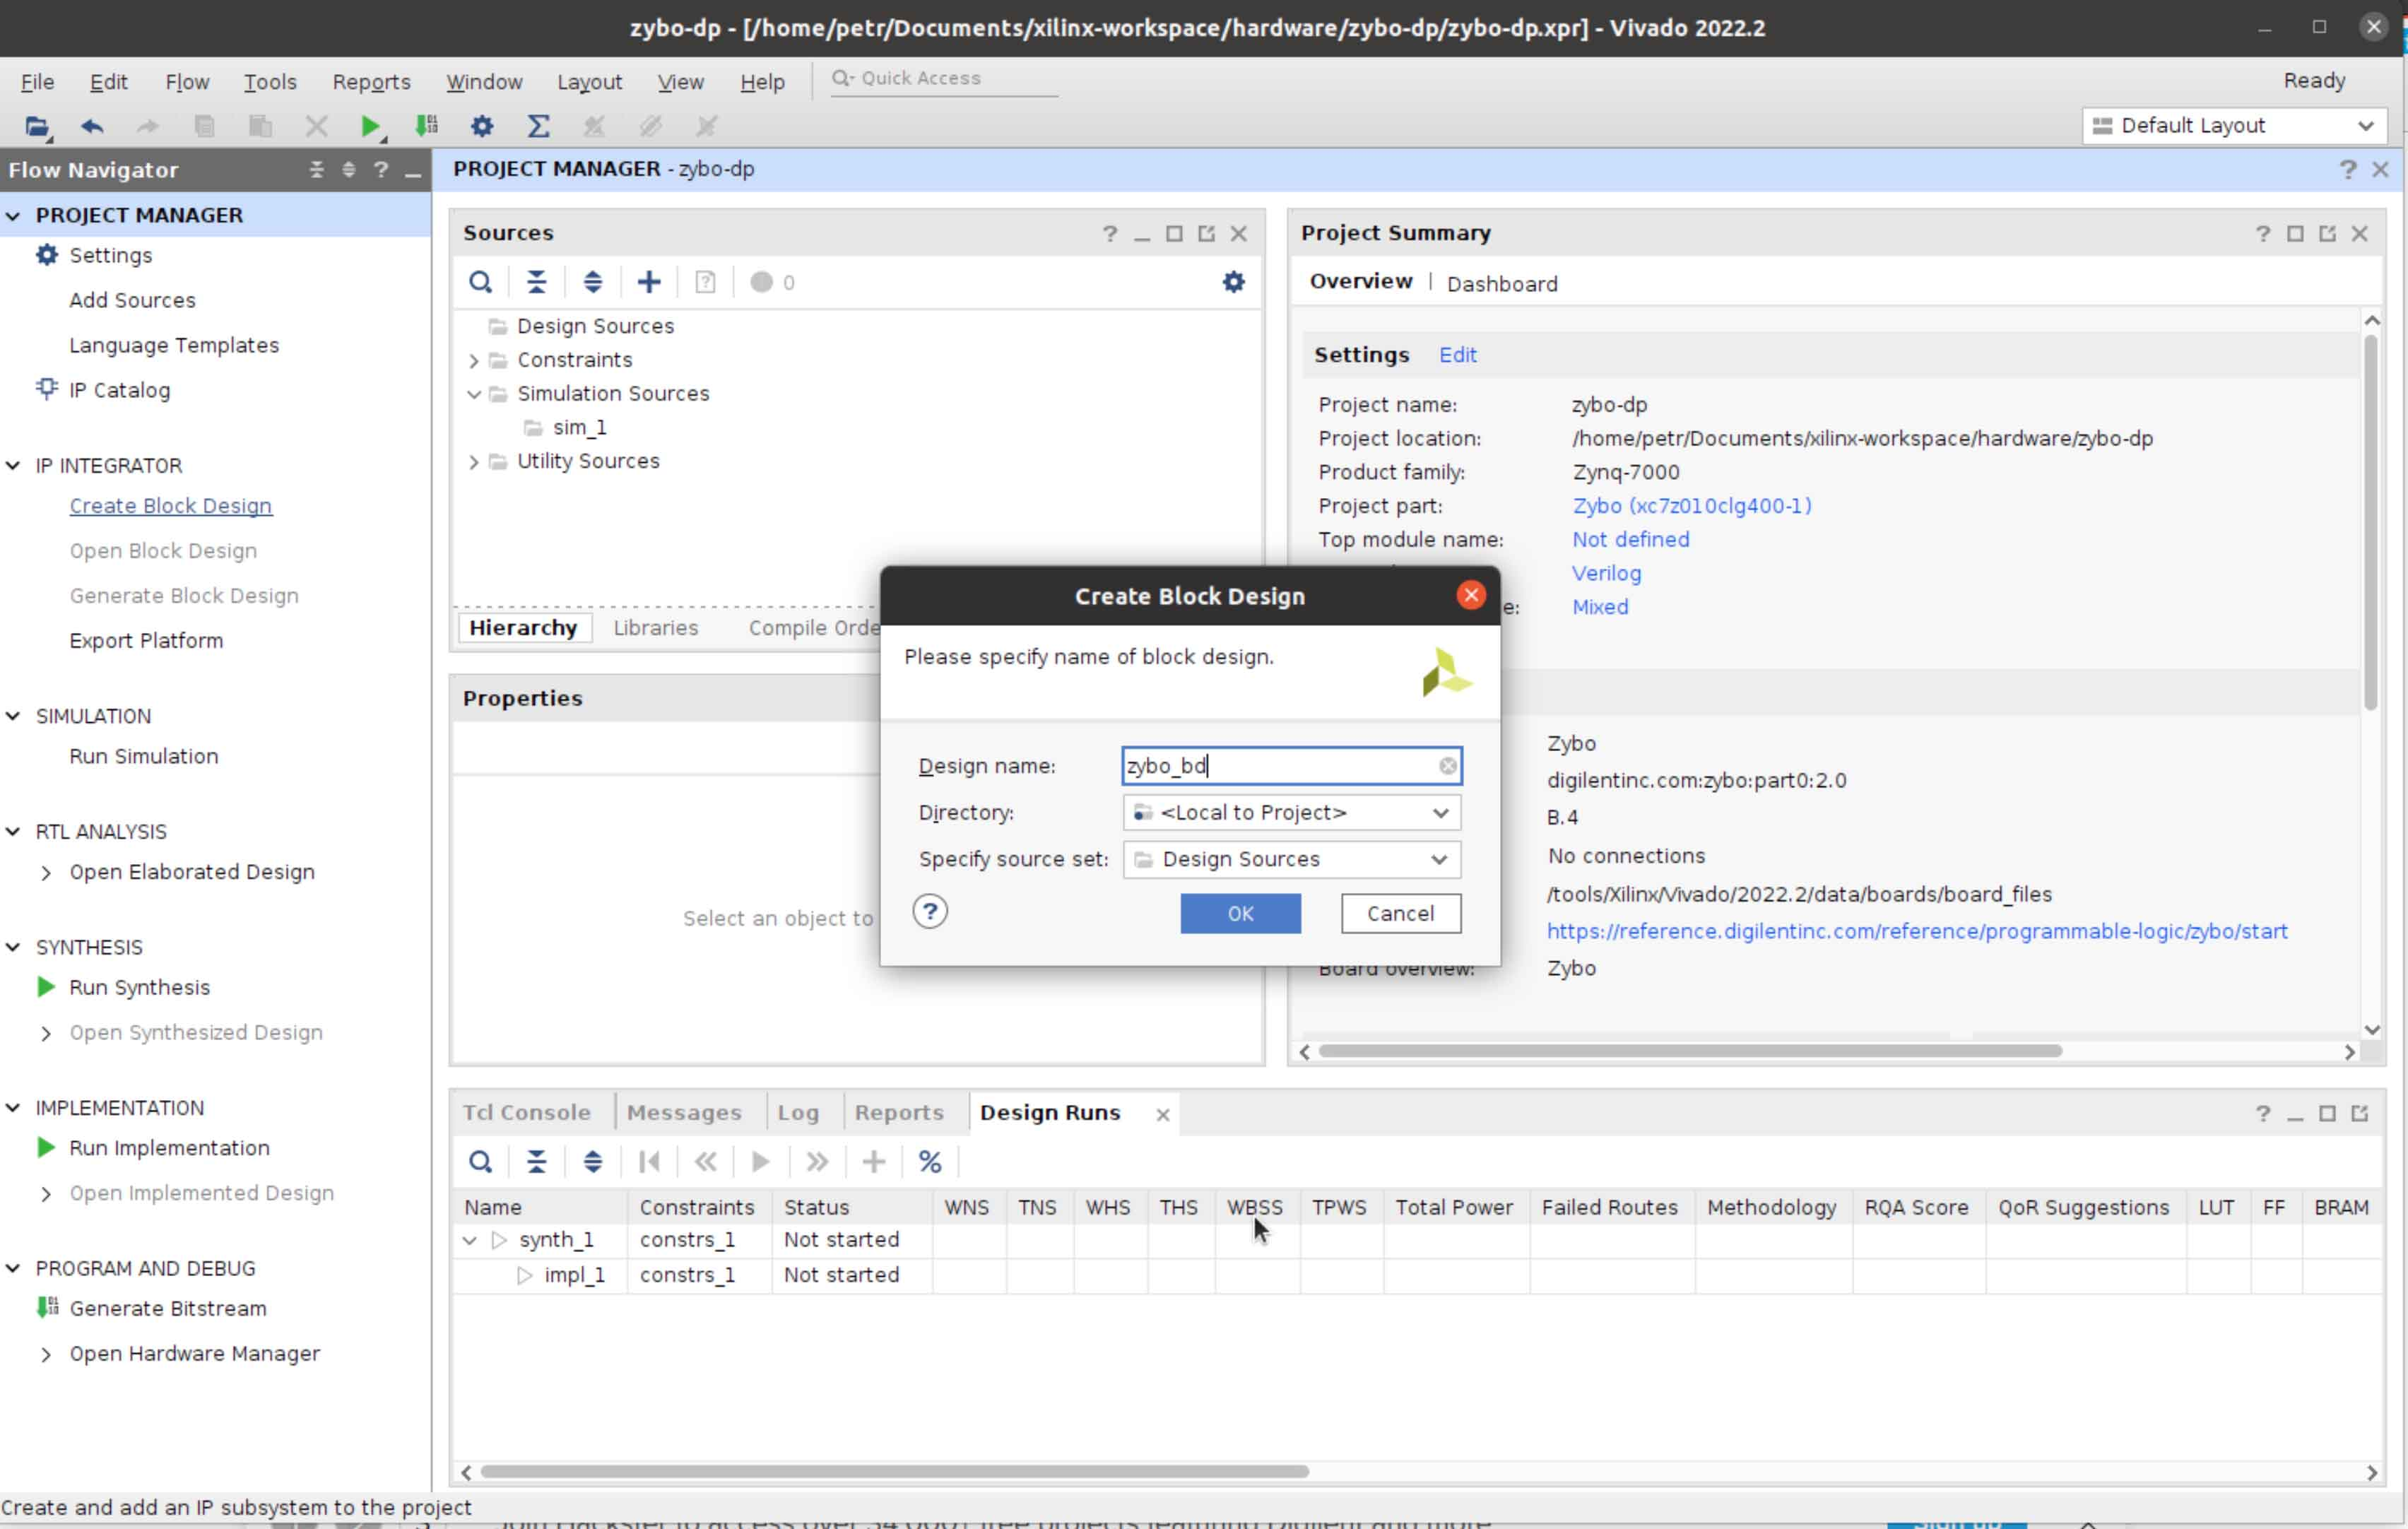
\includegraphics[width=0.75\textwidth]{src/png/zybo-xilinx-vivado-flow/zybo-xilinx-vivado-flow-05.jpg}
			\caption{Xilinx Vivado – vytváření Block Design pro Digilent Zybo.}
			\label{fig:zybo-xilinx-vivado-flow-05}
		\end{figure}

		Nyní je možné již přistoupit k tvorbě vlastní architektury. Prvotním krokem tvorby fesignu je vložit blok \textit{ZYNQ7 Processing System} a zvolit nově zobrazenou možnost \textit{Run Block Automation}. V~těchto pomocných automatizacích je většinou výhodné ponechávat nastavené výchozí hodnoty, které jsou pro většinu tvořeného HW designu dostačující. Menu s~výběrem IP bloku ZynQ PS je zobrazeno na obr. \ref{fig:zybo-xilinx-vivado-flow-07}.

		\begin{figure}[htbp!]
			\centering
			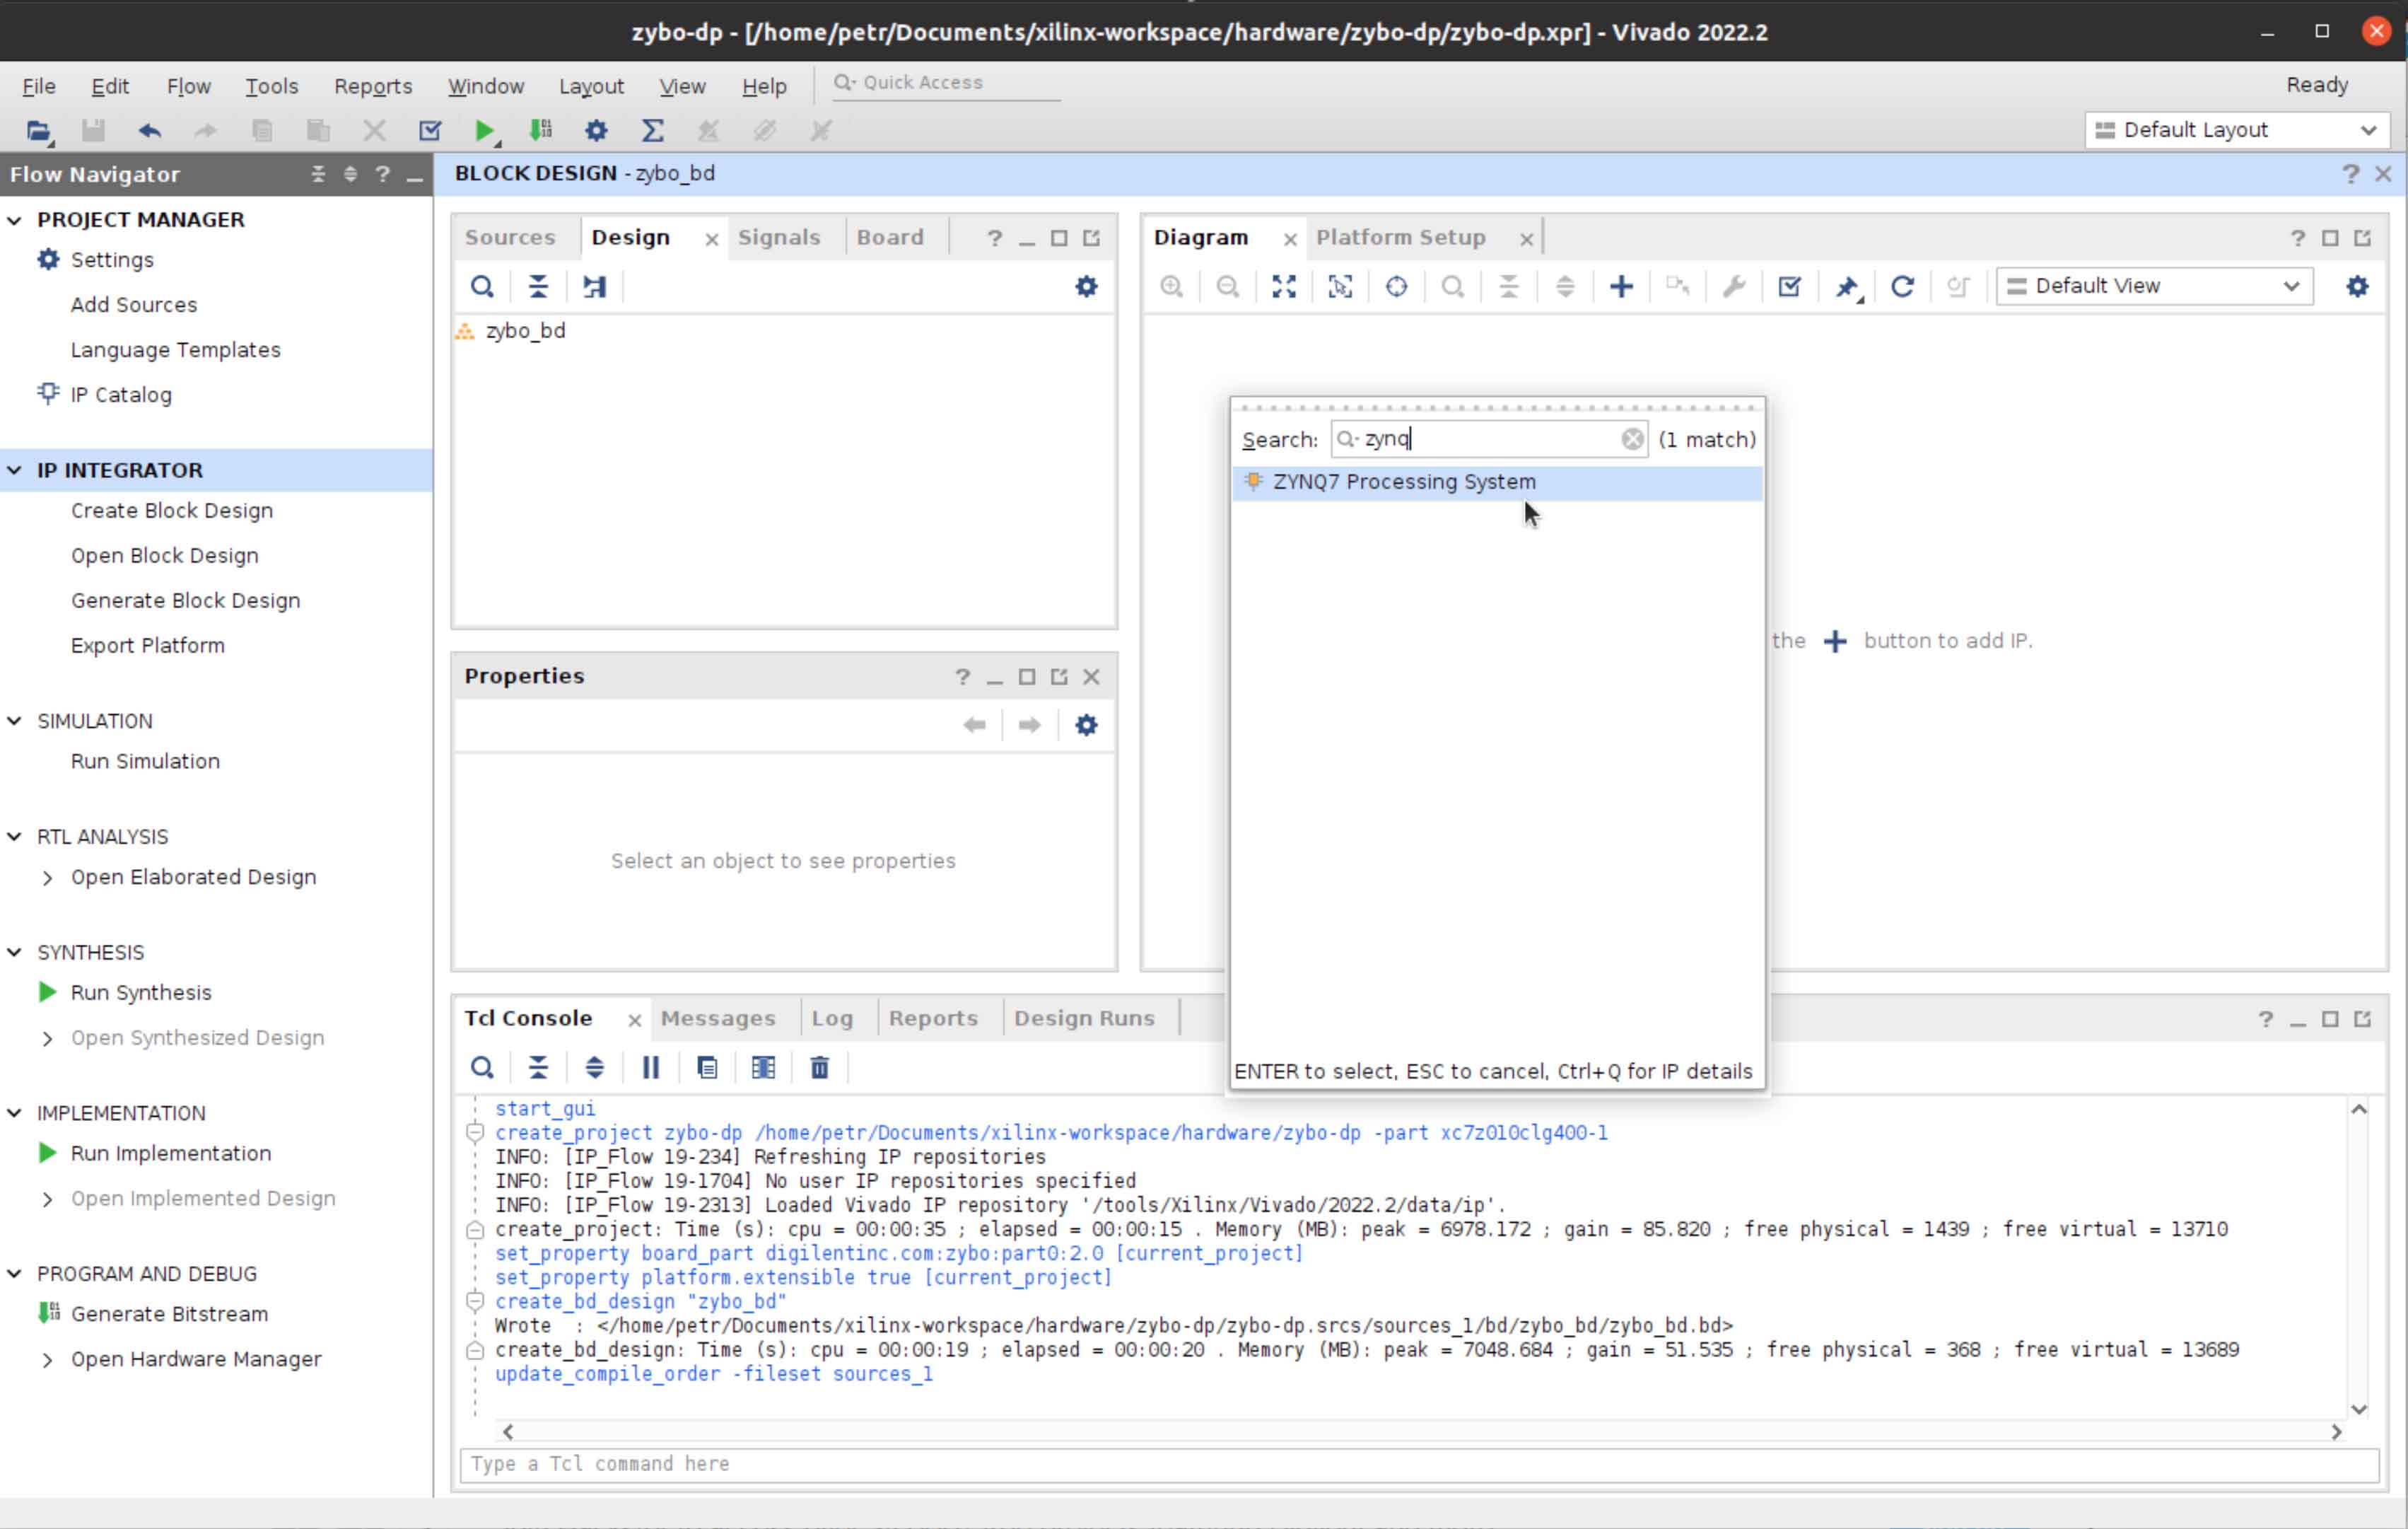
\includegraphics[width=0.75\textwidth]{src/png/zybo-xilinx-vivado-flow/zybo-xilinx-vivado-flow-07.jpg}
			\caption{Xilinx Vivado – vložení bloku ZYNQ7 Processing System pro Digilent Zybo.}
			\label{fig:zybo-xilinx-vivado-flow-07}
		\end{figure}


		Následně je pro funkční akcelerované aplikace nutné vložit do designu blok \textit{Clocking Wizard}, ve kterém nastavit v~záložce \textit{Output Clocks}, aby byl signál aktivní v~0 a aktivovat pět výstupních signálů \textit{Clock}. Těmto signálům je po aktivaci možné nastavit taktovací frekvenci na 50, 100, 150, 200 a 300 Hz. Poté je nutné na výstup \textit{FCLK\_CLK0} bloku \textit{ZYNQ7 Processing System} připojit vstup \textit{clk\_in1} a k~výstupu \textit{FCLK\_RESET0\_N} vstup \textit{resetn}.\par
		Po nastavení bloku \textit{Clocking Wizard} je zapotřebí do designu vložit pět bloků \textit{Processor System Reset}. Následuje propojení odpovídajících výstupů bloků \textit{Clocking Wizard} s~názvem \textit{clk\_outX}, kde \textit{X} značí pořadí výstupního signálu, s~odpovídajícímí bloky \textit{Processor System Reset} a jejich vstupy \textit{slowest\_sync\_clk}. Ke všem vstupům \textit{dcm\_locked} bloků \textit{Processor System Reset} je nutné připojit výstup \textit{locked} \textit{Clocking Wizard}. A~konečně ke všem vstupům \textit{ext\_reset\_in} připojit výstup \textit{FCLK\_RESET0\_N} ZynQ bloku. Představené propojení jednotlivých bloků je možné pozorovat na obr. \ref{fig:zybo-xilinx-vivado-flow-12}.

		\begin{figure}[htbp!]
			\centering
			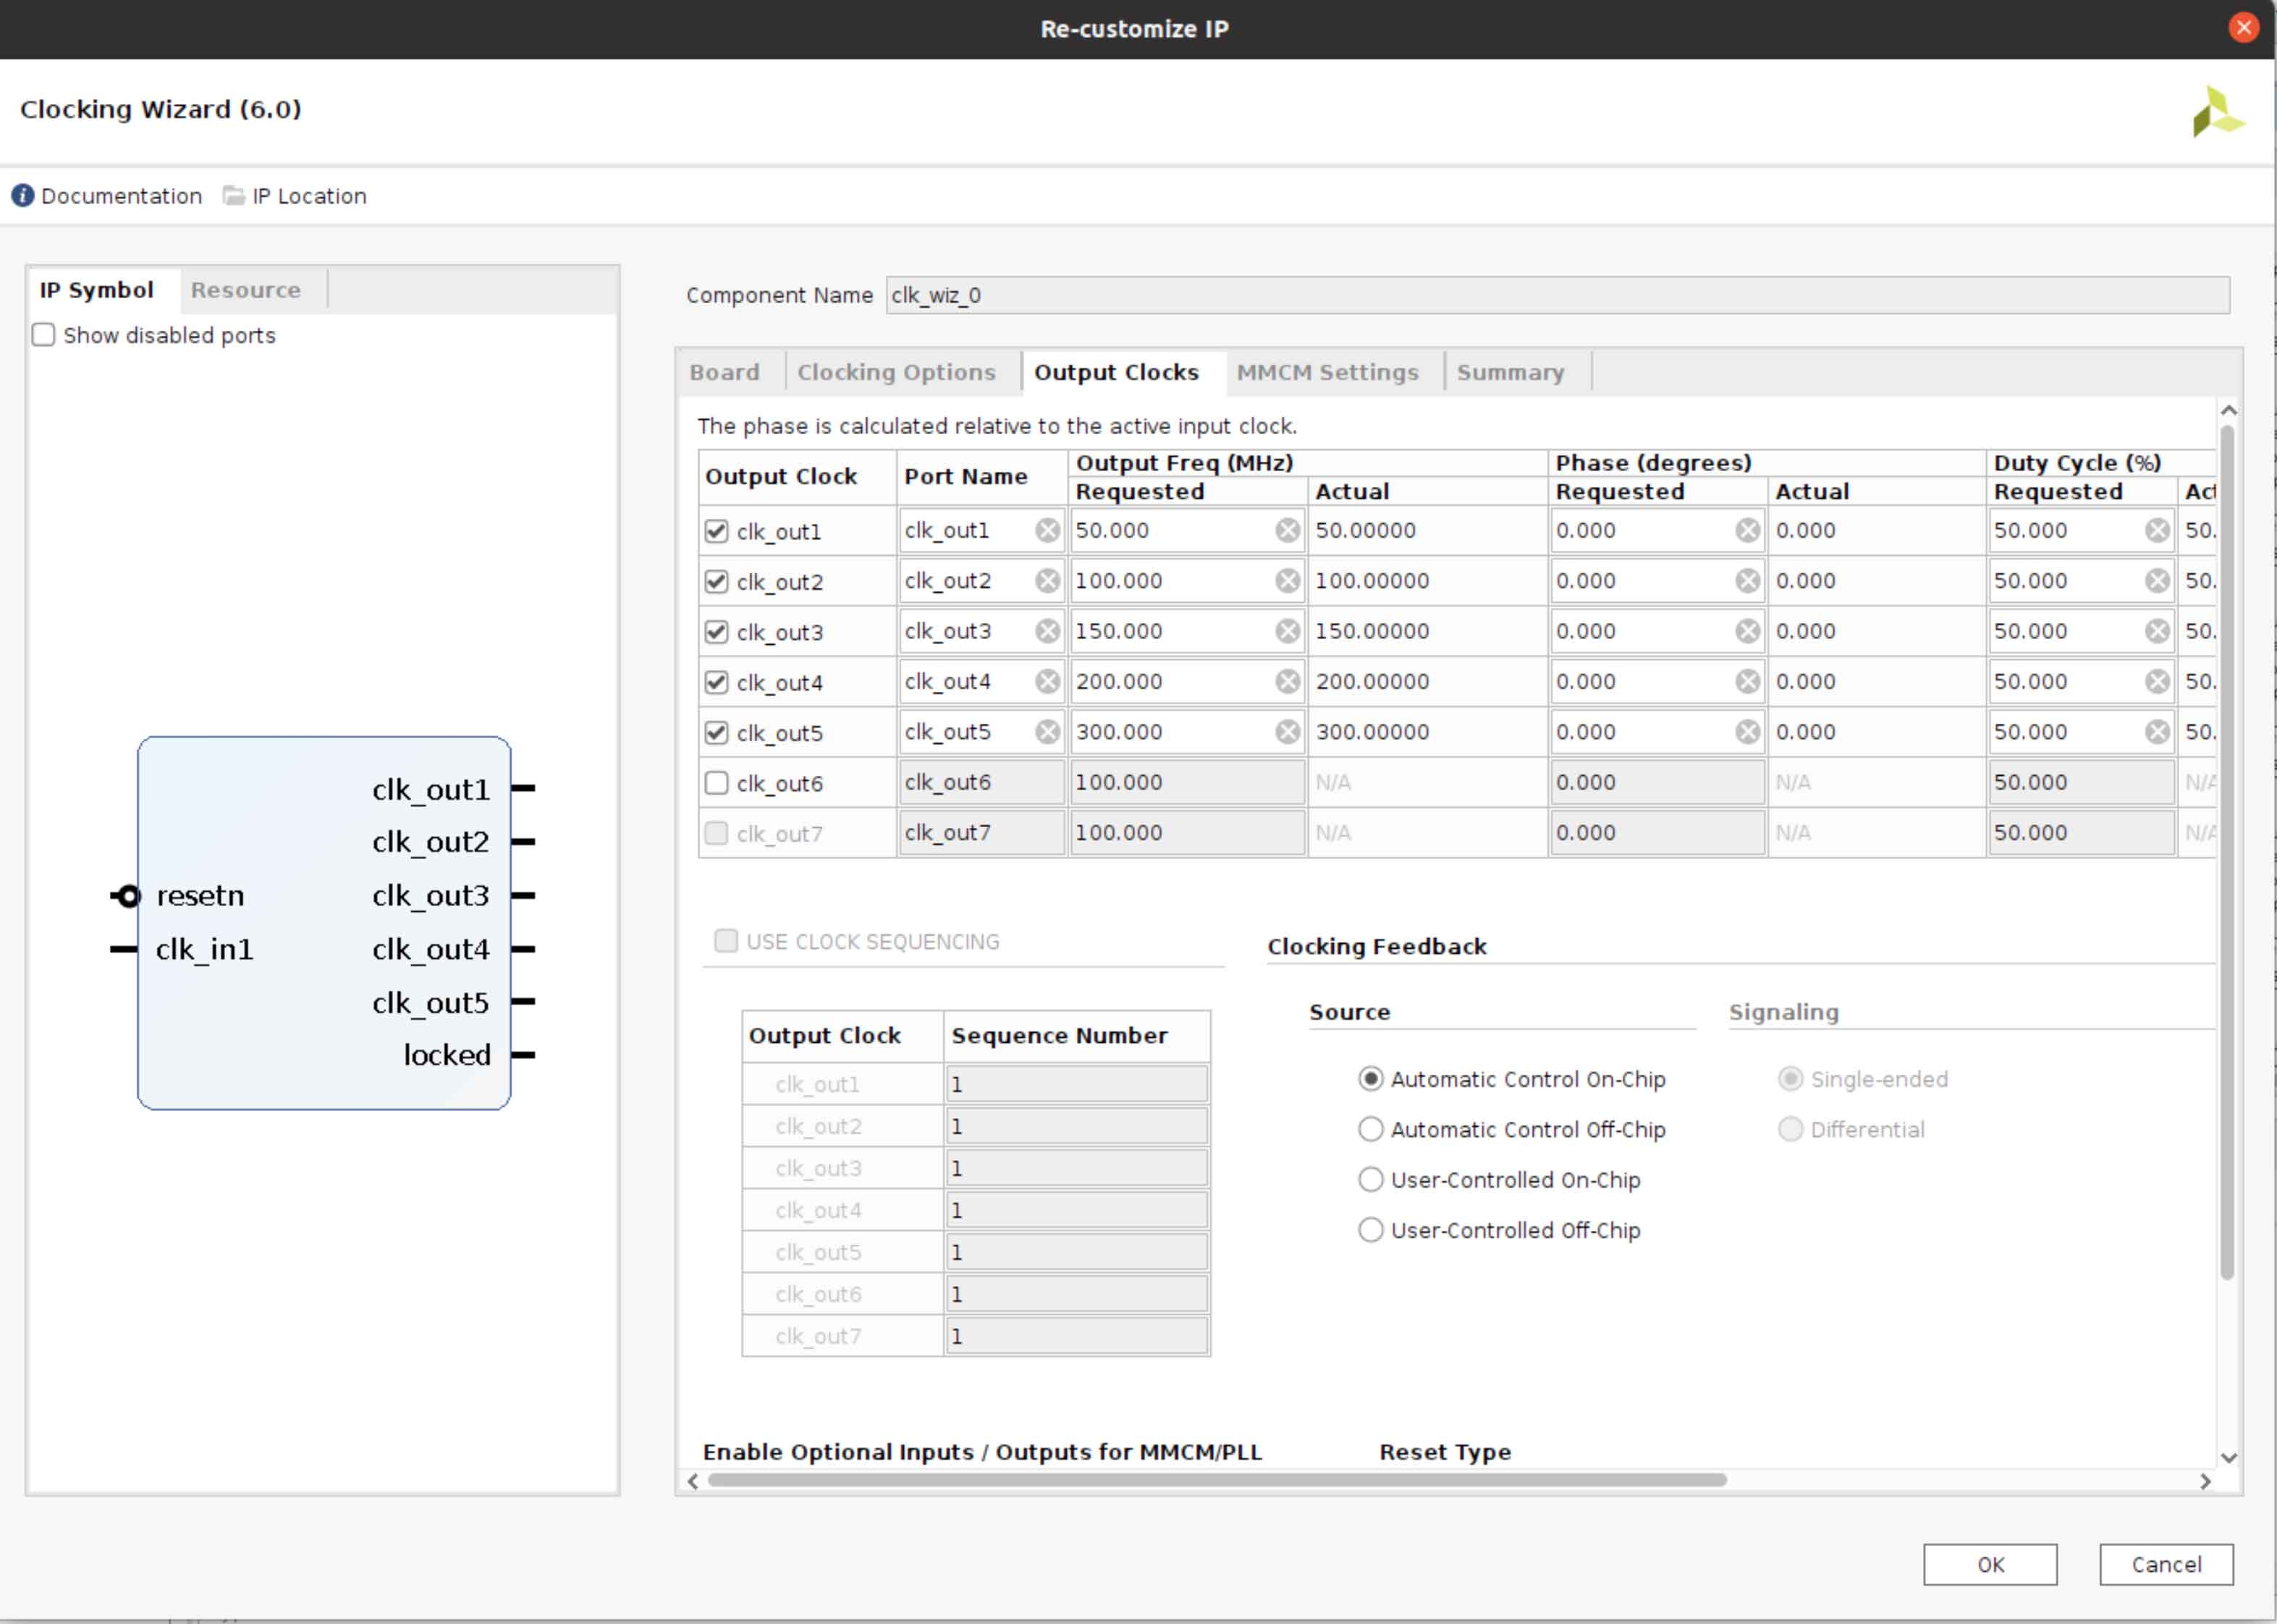
\includegraphics[width=0.75\textwidth]{src/png/zybo-xilinx-vivado-flow/zybo-xilinx-vivado-flow-36.jpg}
			\caption{Xilinx Vivado – nastavení výstupních taktovacích signálů pro Digilent Zybo.}
			\label{fig:zybo-xilinx-vivado-flow-36}
		\end{figure}

		\begin{figure}[htbp!]
			\centering
			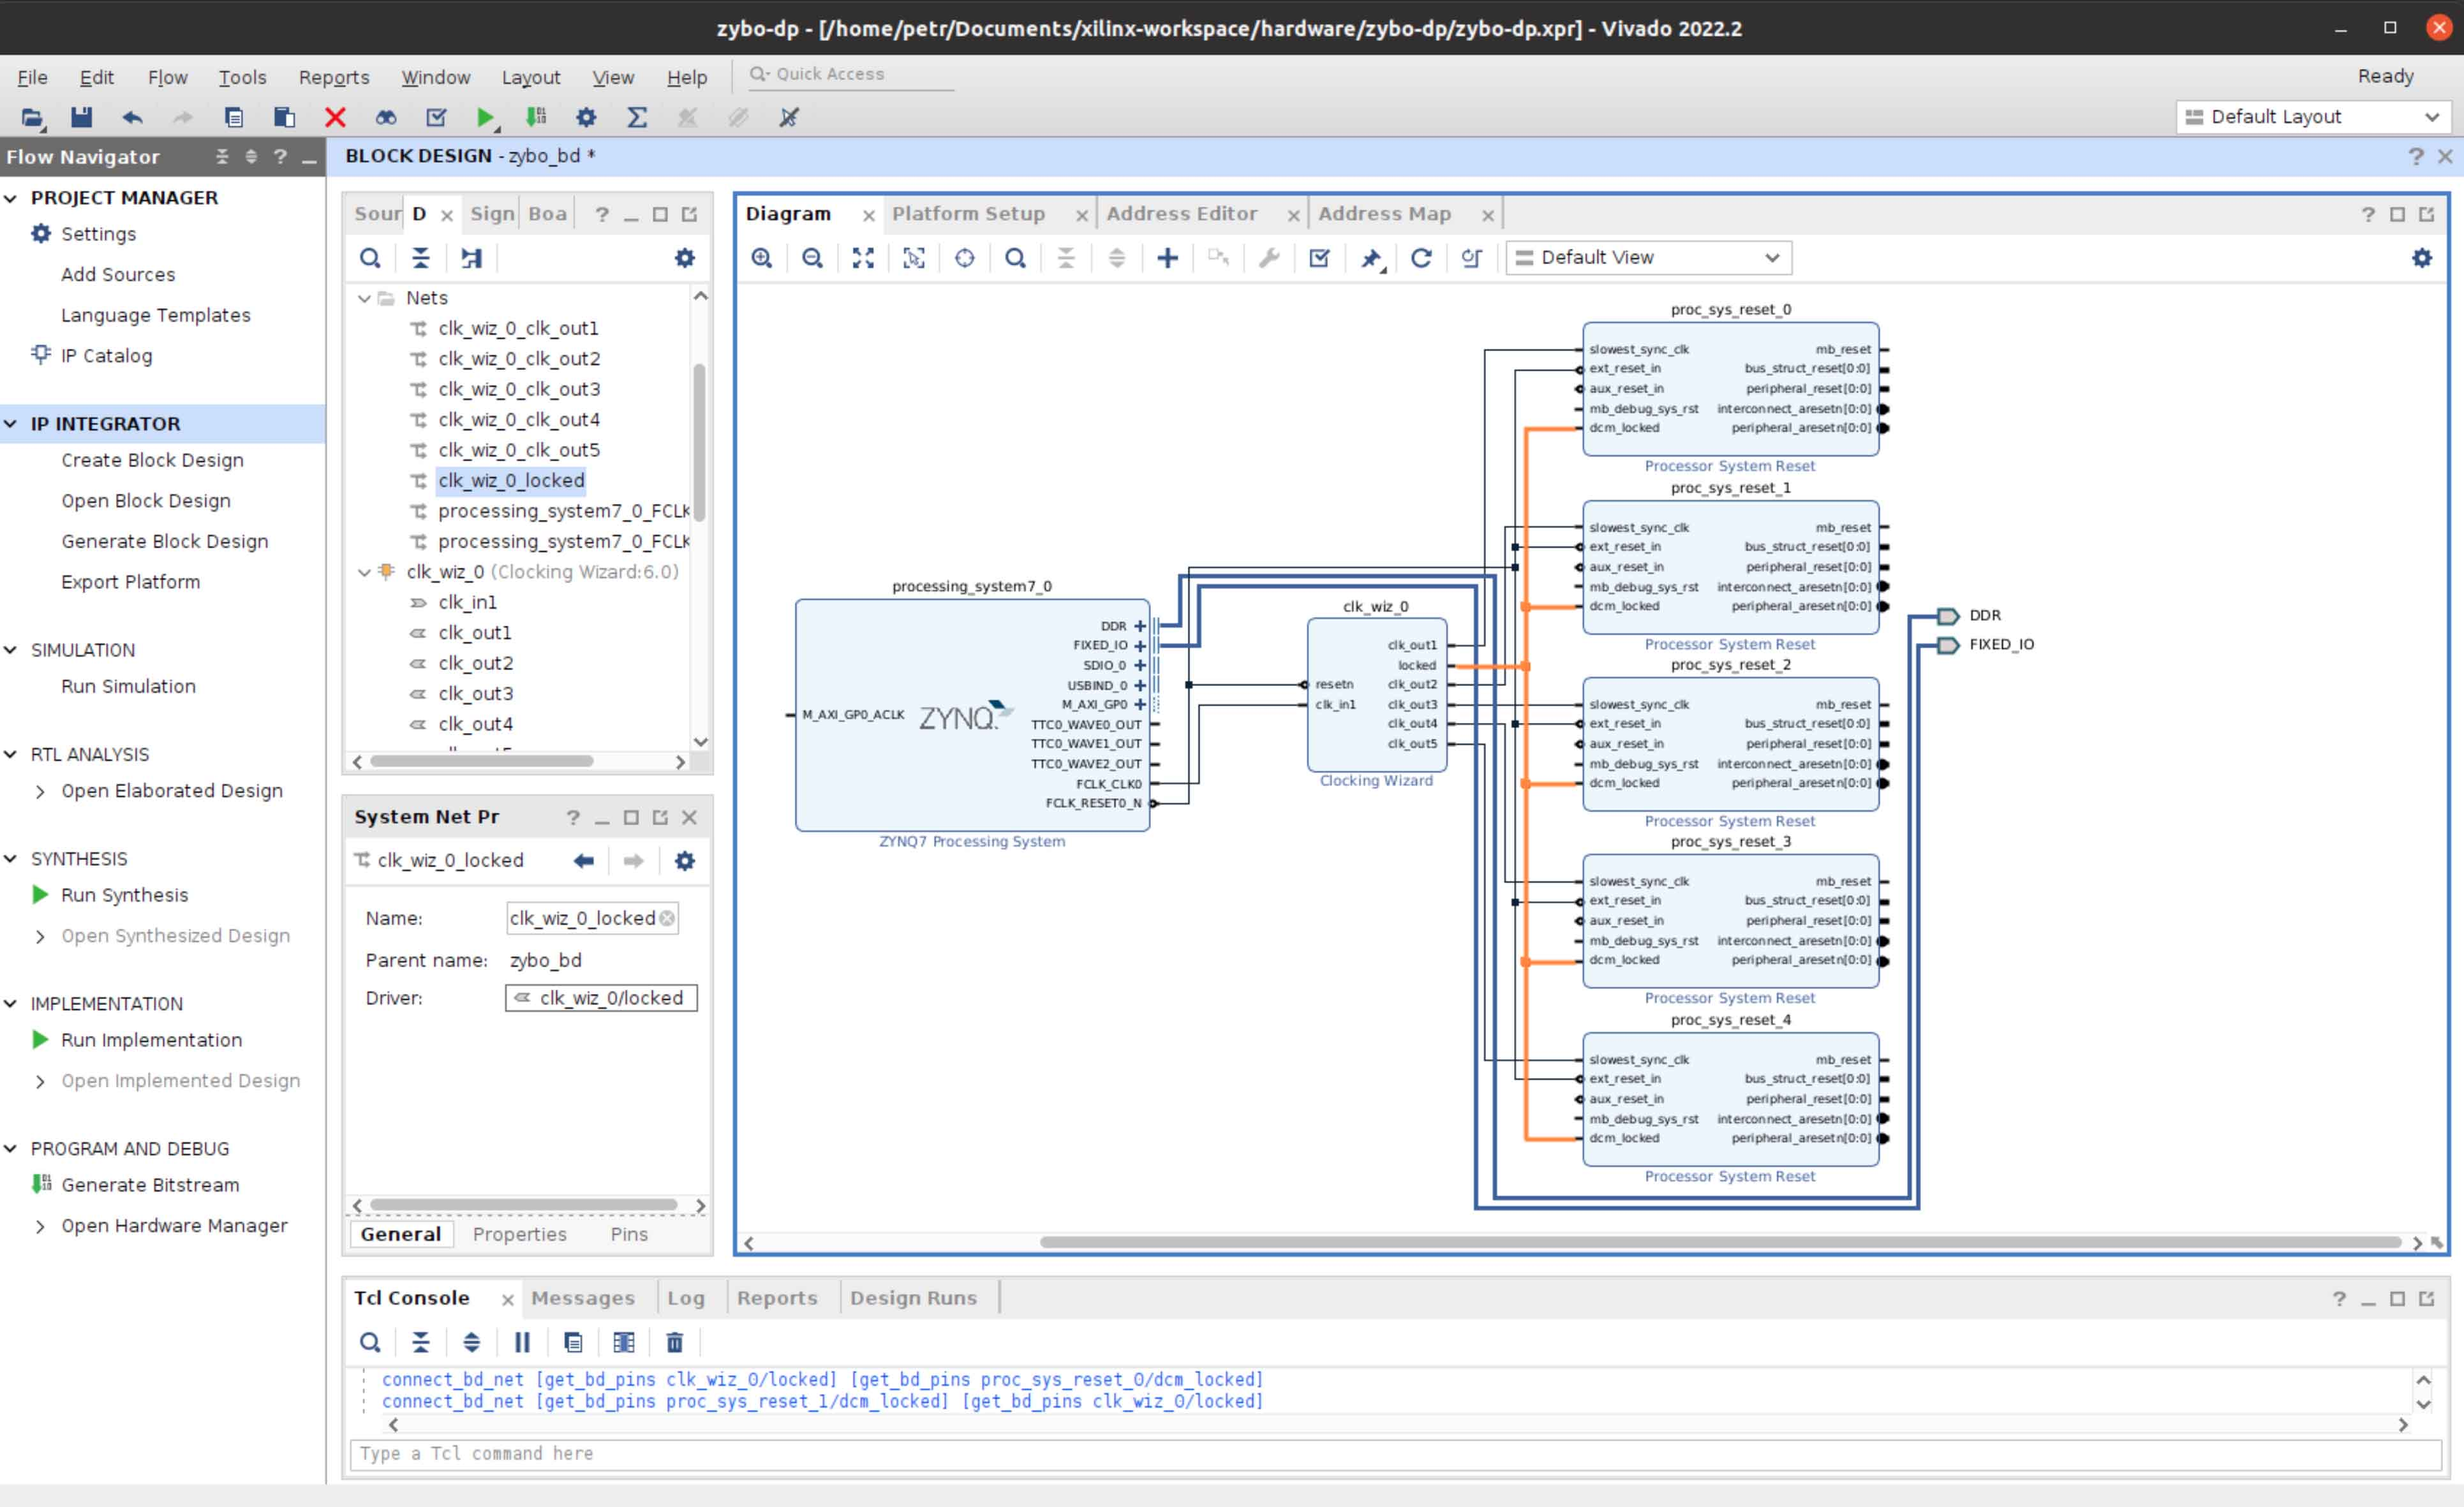
\includegraphics[width=0.85\textwidth]{src/png/zybo-xilinx-vivado-flow/zybo-xilinx-vivado-flow-12.jpg}
			\caption{Xilinx Vivado – propojení bloků taktování pro Digilent Zybo.}
			\label{fig:zybo-xilinx-vivado-flow-12}
		\end{figure}

		\fbar

		Nyní je možné otevřít nastavení \textit{ZYNQ7 Processing System} a v~záložce \textit{Interrupts} povolit nastavení \textit{Fabric Interrupts/PL-PS Interrupt Ports/IRQ\_F2P} přerušení. Následně do designu je nutné vložit blok řídící přerušení se jménem \textit{AXI Interrupt Controller}, otevřít jeho nastavení a v~sekci \textit{Processor Interrupt Type and Connection} změnit nastavení \textit{Interrupt Output Connection} z~\textit{Bus} na \textit{Single}. Následně je opět možné spustit automatické propojení jednotlivých bloků s~výchozím nastavením.\par
		Aby byly přerušení funkční, je třeba propojit výstup bloku \textit{AXI Interrupt Controller} se jménem \textit{irq} se vstupem bloku \textit{ZYNQ7 Processing System} \textit{IRQ\_F2P}. Minimální funkční blokový design je zobrazen na obr. \ref{fig:zybo-xilinx-vivado-flow-17}.

		\begin{figure}[htbp!]
			\centering
			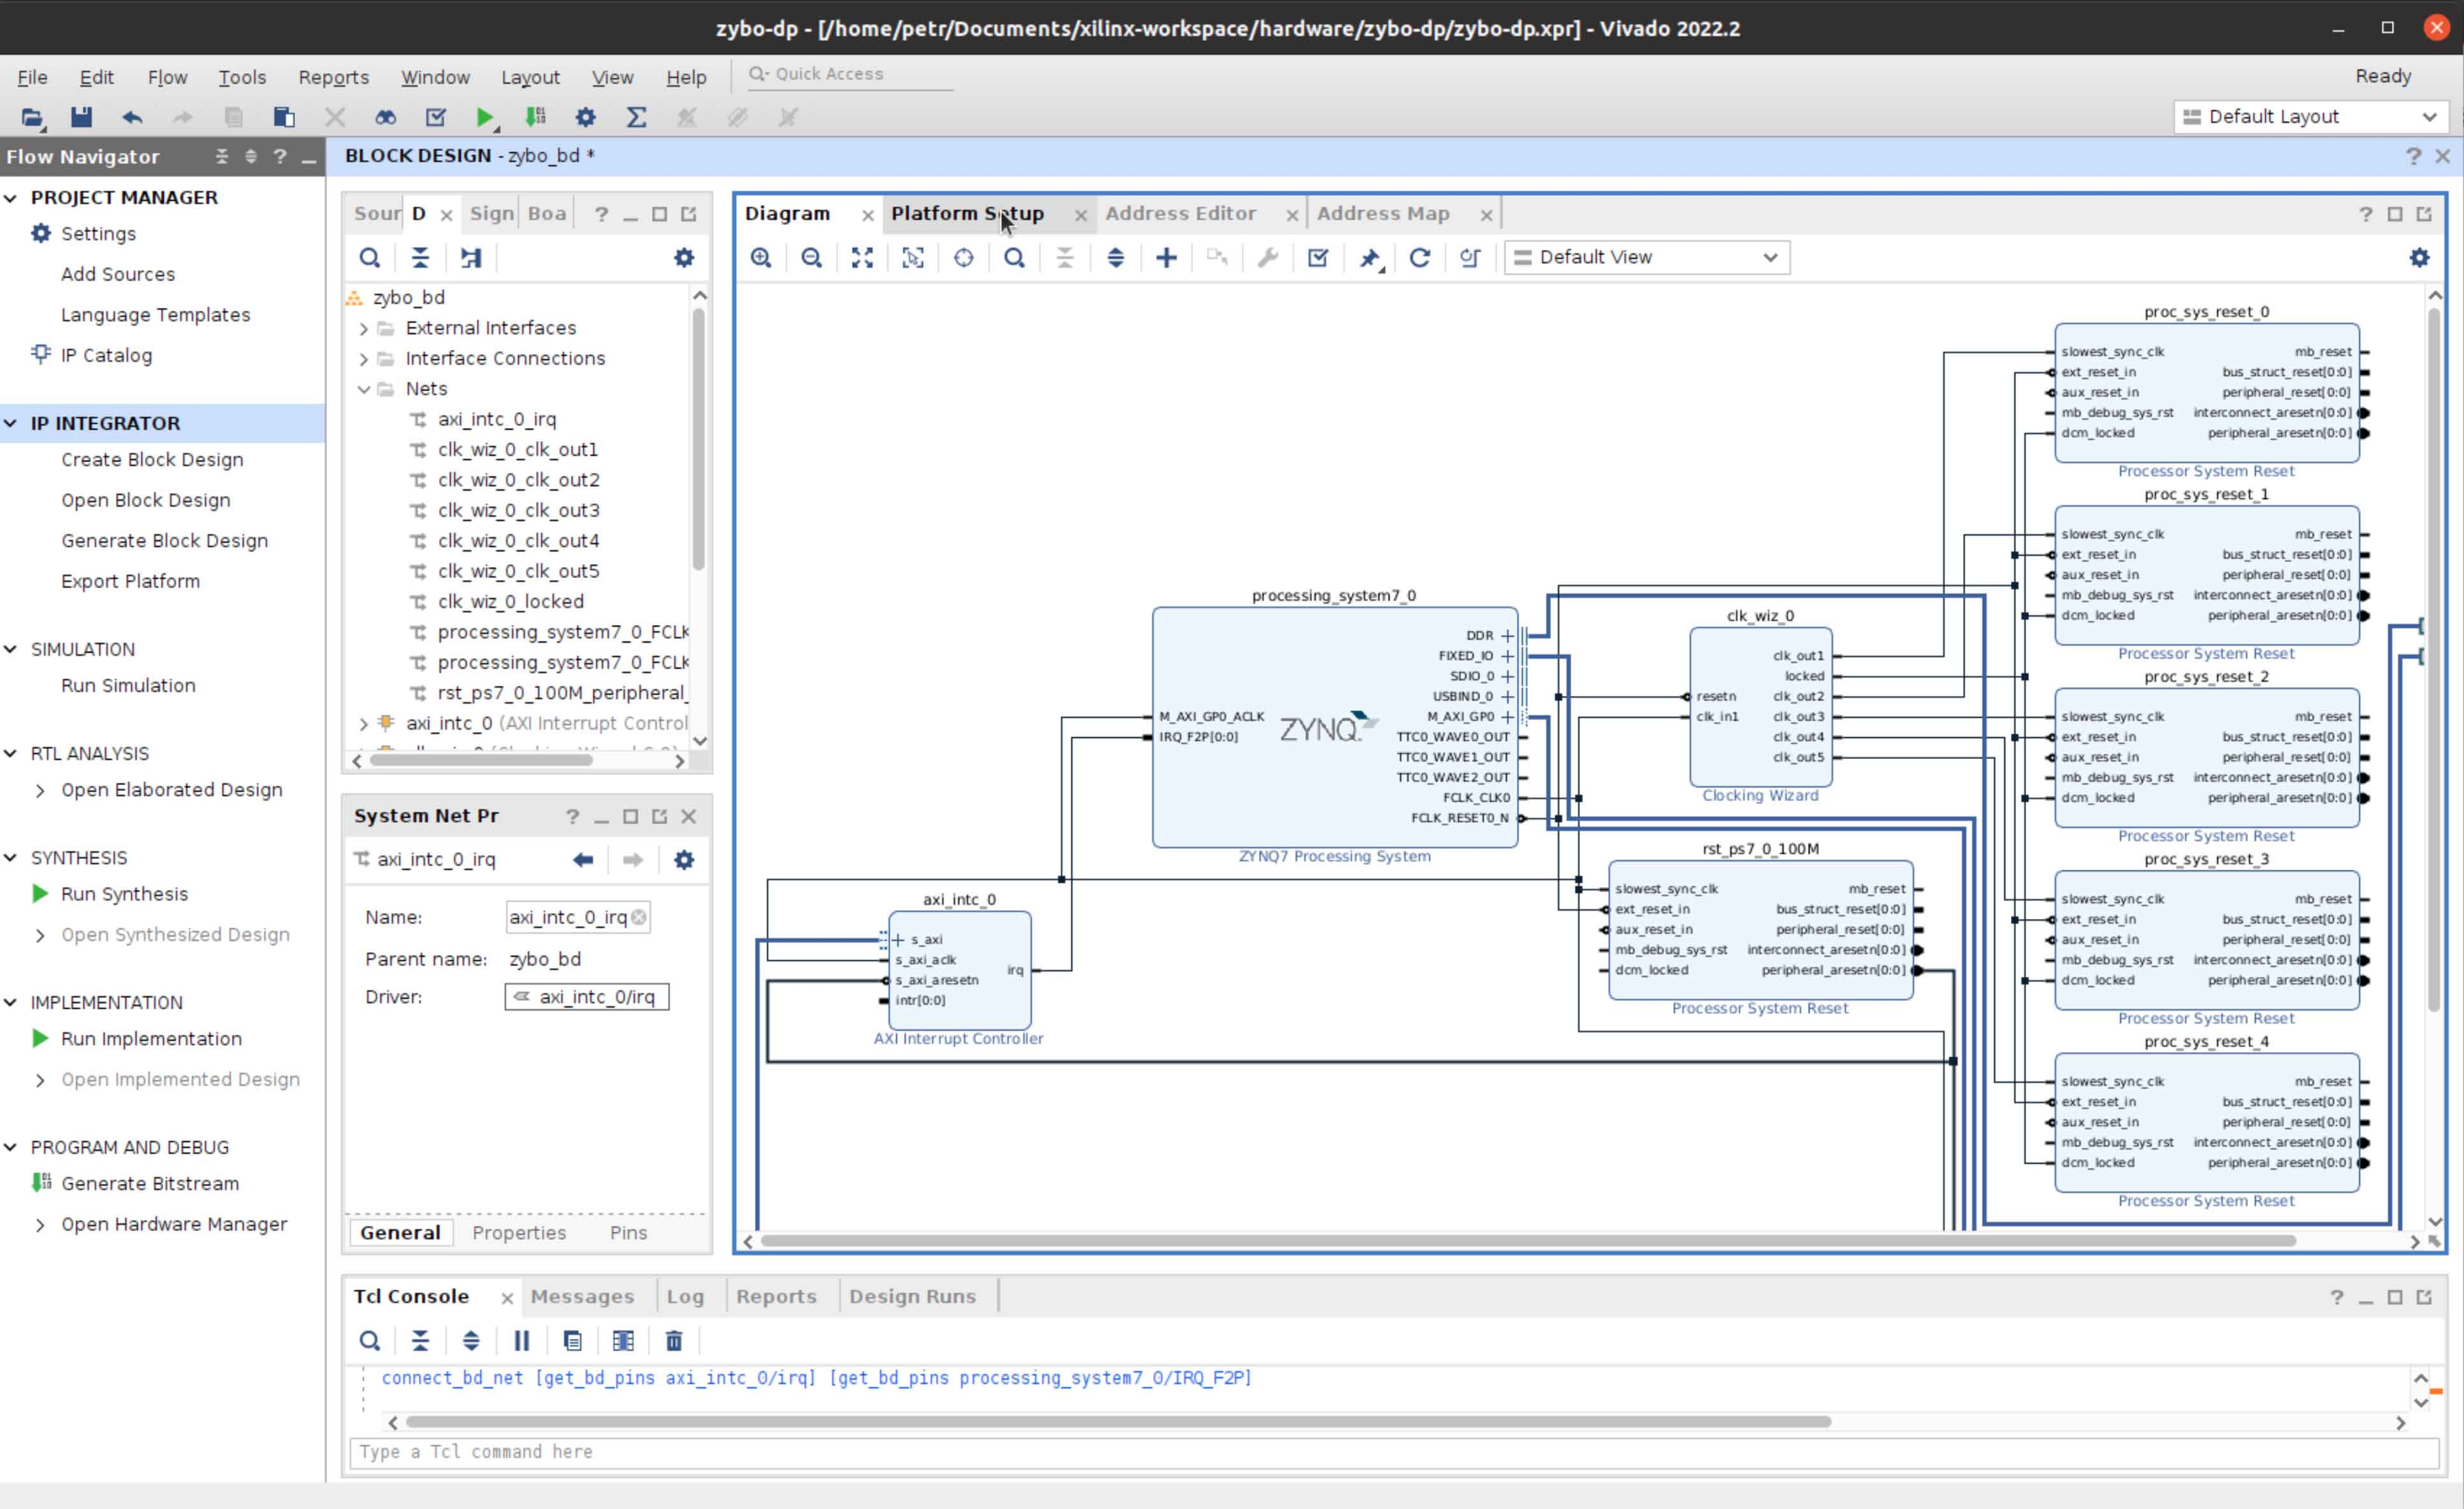
\includegraphics[width=0.85\textwidth]{src/png/zybo-xilinx-vivado-flow/zybo-xilinx-vivado-flow-17.jpg}
			\caption{Xilinx Vivado – minimální funkční blokový design pro akcelerovanou aplikaci pro Digilent Zybo.}
			\label{fig:zybo-xilinx-vivado-flow-17}
		\end{figure}

		Nyní je možné přejít ze záložky \textit{Diagram} do záložky \textit{Platform Setup} ve které je pro zajištění funkčnosti nutné nastavit určité potřebné konektory a výstupy. Následuje nastavení parametrů bloku \textit{ZYNQ7 Processing System} v~záložce \textit{AXI Port} dle tabulky č. \ref{tab:vivado-platform-setup-axi-digilent-zybo}.


		\begin{table}[H]
			\centering
			\caption{Ukázka nastavených AXI portů v~Xilinx Vivado platformě pro \textit{Digilent Zybo}.}
		  \vspace*{0.15cm}
		
			\begin{tabular}{!{\vrule width 2pt} c | c | c | c !{\vrule width 2pt}}
			\noalign{\hrule height 2pt}
			Name & Enabled & Memport & SP Tag\\
			\noalign{\hrule height 2pt}
			M\_AXI\_GP1 & X & M\_AXI\_GP & -\\ \hline
			S\_AXI\_ACP & O~& - & - \\ \hline
			S\_AXI\_HP0 & X & S\_AXI\_HP & HP0 \\ \hline
			S\_AXI\_HP1 & X & S\_AXI\_HP & HP1 \\ \hline
			S\_AXI\_HP2 & X & S\_AXI\_HP & HP2 \\ \hline
			S\_AXI\_HP3 & X & S\_AXI\_HP & HP3 \\\noalign{\hrule height 2pt}
			\end{tabular}
			\label{tab:vivado-platform-setup-axi-digilent-zybo}
		\end{table}

		Aby bylo možné zapisovat do globální paměti přes MAXI Adapter je nutné povolit funkci vybraných portů v~bloku \textit{AXI Interconnect}. V~této práci byly povoleny porty \textit{M01\_AXI} až \textit{M32\_AXI}.\par
		Následně v~záložce \textit{Clock} je nutné povolit \textit{clk\_outx}, kde $x \in <1,5>$, nastavit jejich odpovídající ID a jako výchozí použít taktovací signál 100 MHz.\par
		Dále je v~záložce \textit{Interrupt} nutné aktivovat výstup \textit{intr} bloku \textit{AXI Interrupt Controller}.\par
		Aby bylo možné případně provádět HW-emulaci, je nutné v~kartě \textit{Diagram} zvolit blok \textit{ZYNQ7 Processing System} a v~záložce \textit{Block Properties} v~nabídce \textit{SELECTED\_SIM\_MODEL} zvolit možnost tlm. \cite{hackster-vitis-2021-1-embedded-platform-for-zybo-z7-20}\par
		% informace o nefunkcnim emulatoru, pokud se povede spustit, vymazat
		V~této práci nebylo dosaženo funkční SW ani HW simulace pro desku Digilent Zybo z~neznámých důvodů. Pokud byl emulátor QEMU spuštěn zvlášť pomocí příkazové řádky a přes příkaz byly \textit{scp} přesunuty potřebné soubory, jednalo se pouze o~SW simulaci bez připojeného PL a tudíž nebylo možné algoritmy ověřit.\par
		% vsunutý blok, zkontrolovat poté kontinuitu s předchozím textem
		Pro zajištění funkčních GPIO (General Purpose Input/Output) pro ovládání LED signalizace, tlačítek a přepínačů, připojených na PL, je nutné do blokového designu z~karty \textit{Board/Zybo/GPIO} vložit potřebné IP. Po kliknutí pomocí pravého tlačítka myši na vybraný blok je nutné zvolit z~nabídky \textit{Connect board component} a požadovaný GPIO interface. Blok \textit{AXI GPIO} je automaticky vložen do blokového designu a jeho přítomnost je signalizována na kartě \textit{Board/Zybo/GPIO} zvýraznění vložených bloků (ukázka na obr. \ref{fig:zybo-xilinx-vivado-flow-38}). Dle požadavku uživatele je možné vybrat zda bude využíváno \textit{GPIO} nebo \textit{GPIO2} rozhraní. Dle vybraného rozhraní budou poté adresovány jednotlivé výstupy a vstupy v~\textit{Petalinux}. Ukázka vytvořeného designu s IP pro GPIO je na obr. \ref{fig:zybo-xilinx-vivado-flow-37}.


		\begin{figure}[htbp!]
			\centering
			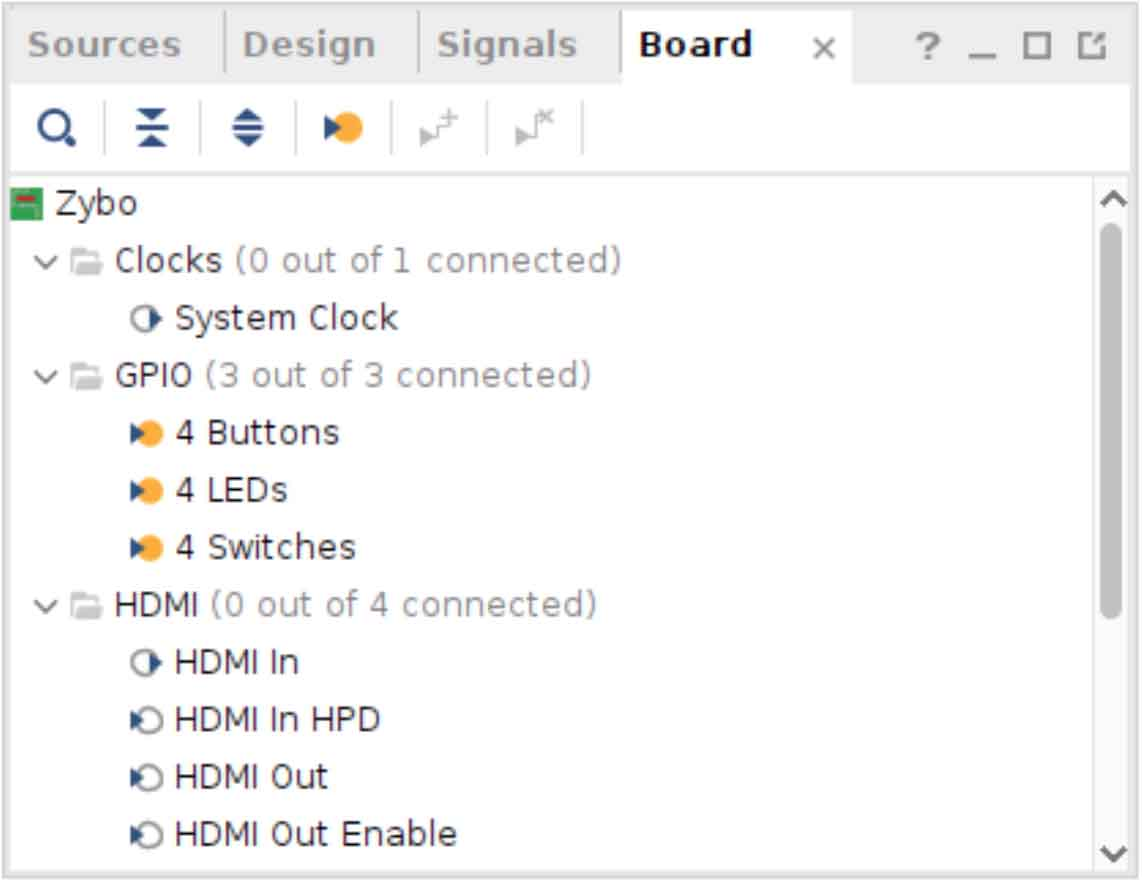
\includegraphics[width=0.65\textwidth]{src/png/zybo-xilinx-vivado-flow/zybo-xilinx-vivado-flow-38.jpg}
			\caption{Xilinx Vivado – signalizace vložených AXI GPIO bloků pro LED, BTN, SW na kartě \textit{Board/Zybo/GPIO} pro Digilent Zybo.}
			\label{fig:zybo-xilinx-vivado-flow-38}
		\end{figure}

		\begin{figure}[htbp!]
			\centering
			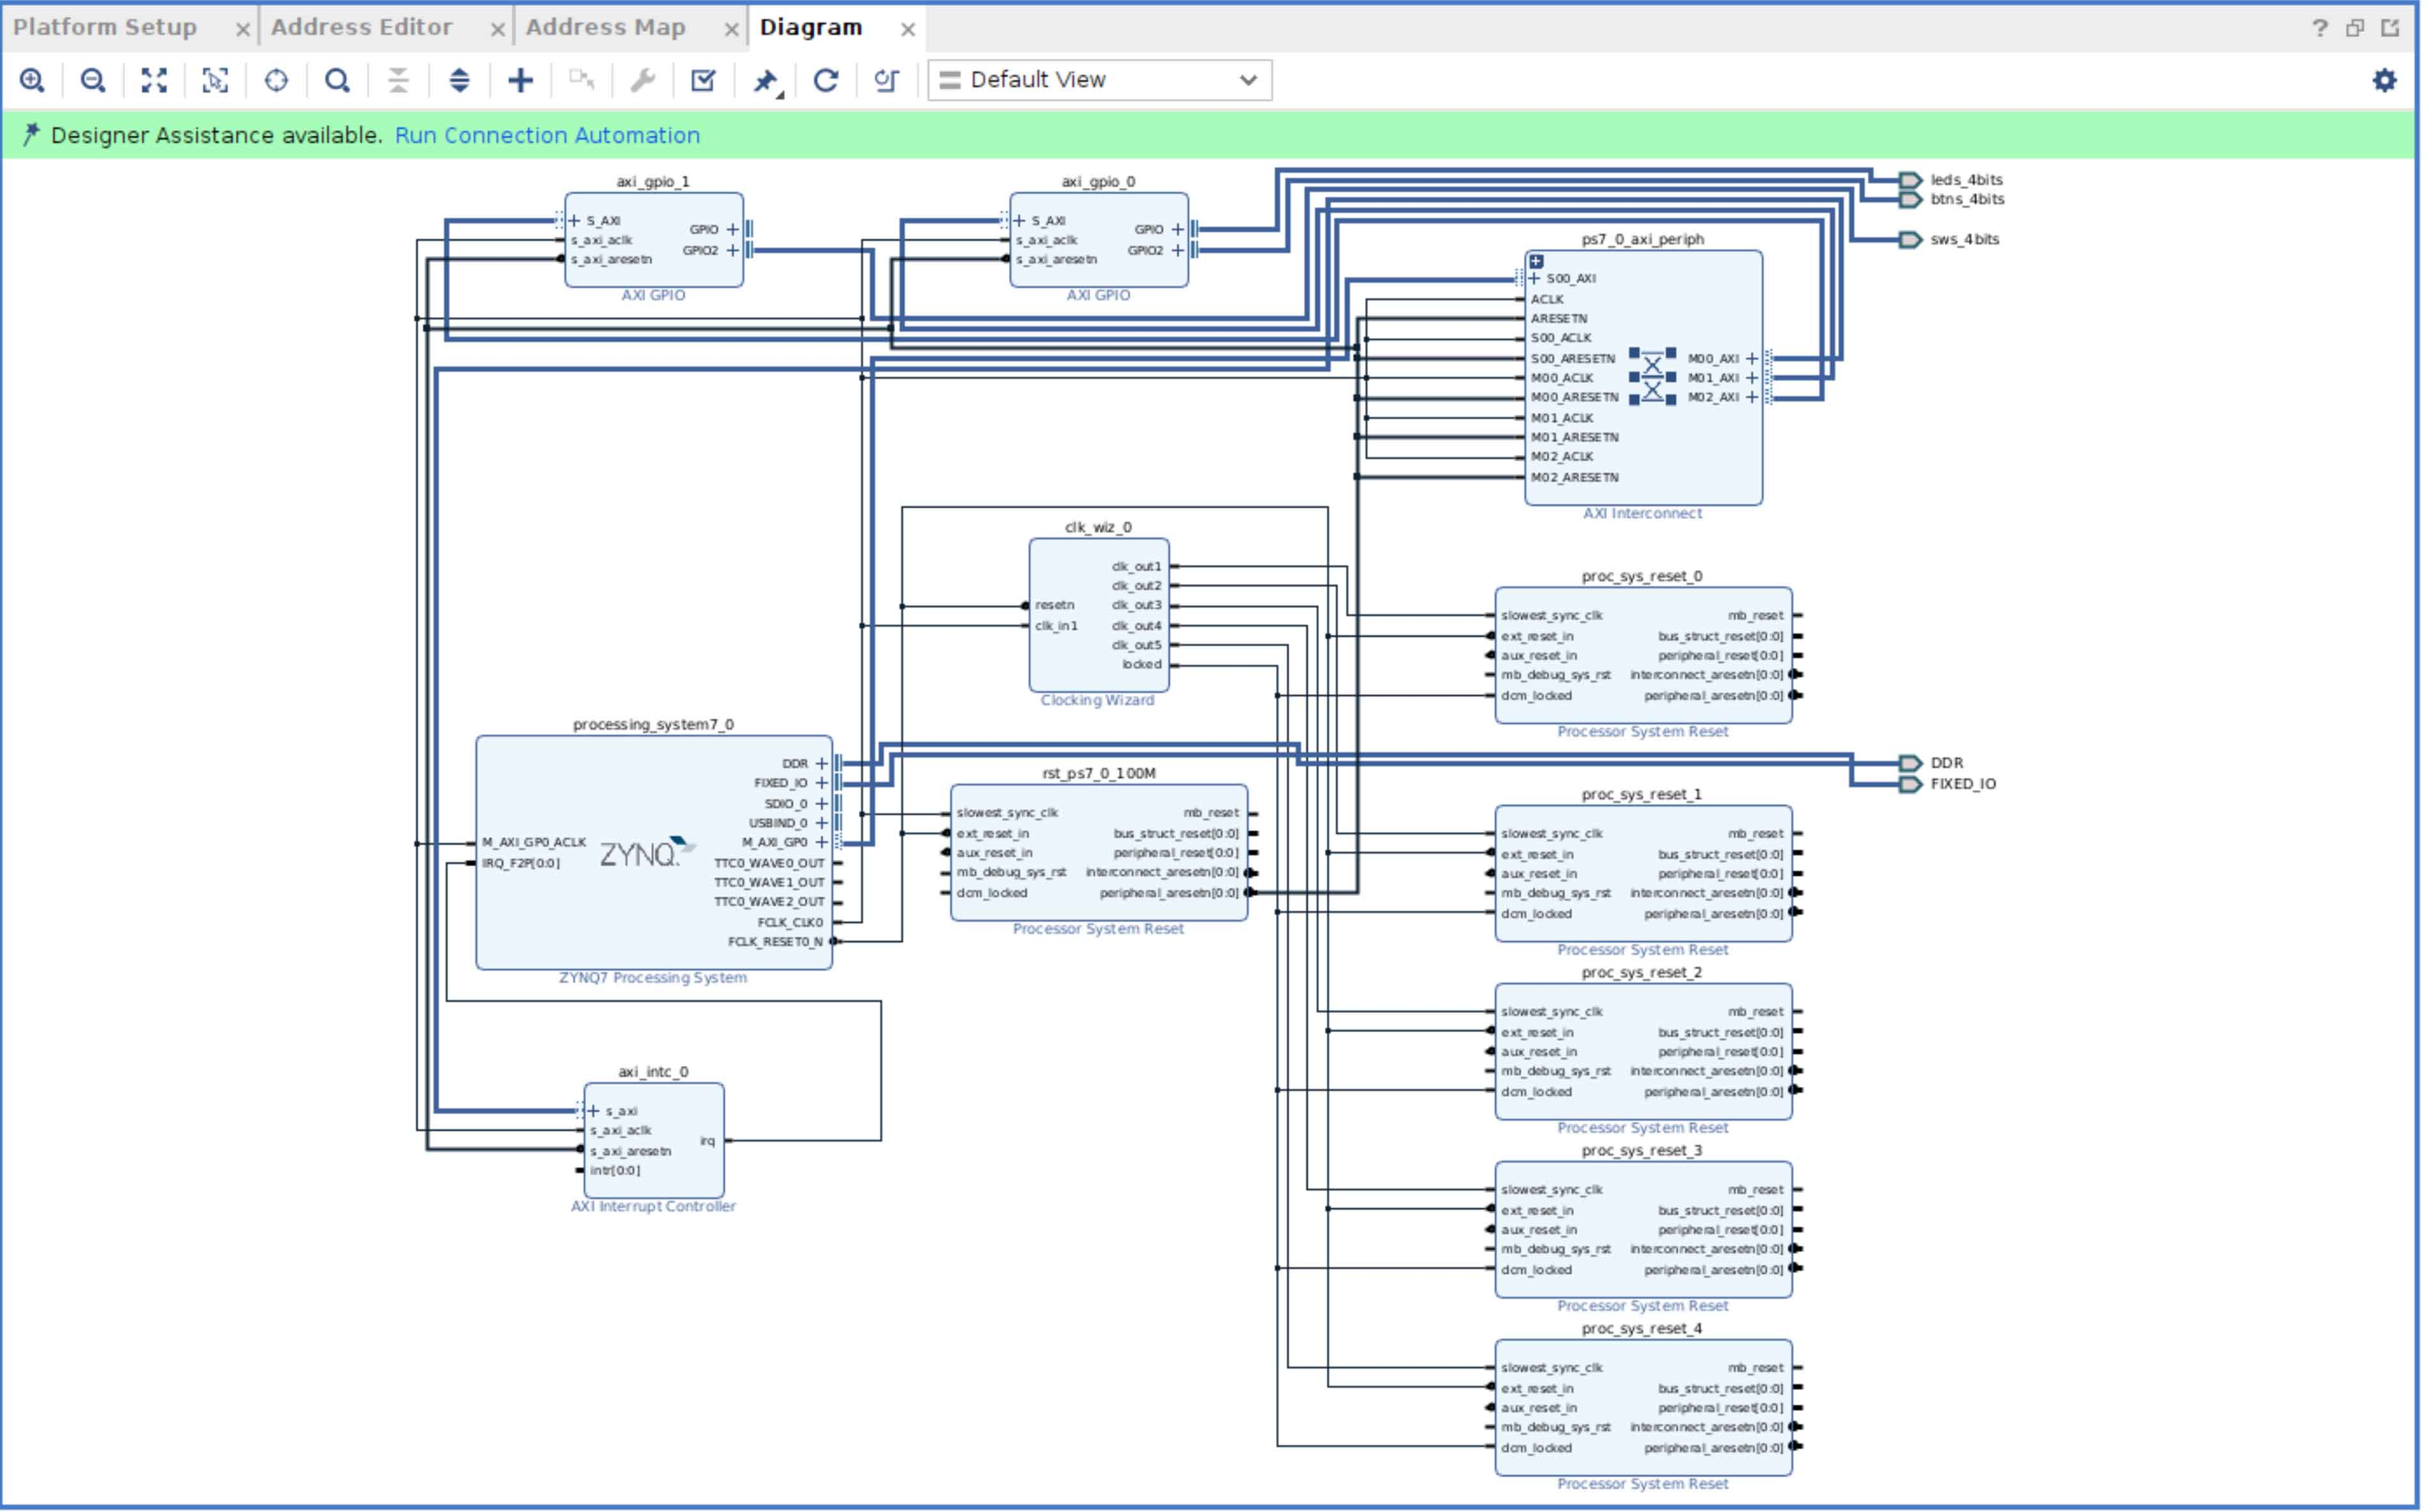
\includegraphics[width=0.95\textwidth]{src/png/zybo-xilinx-vivado-flow/zybo-xilinx-vivado-flow-37.jpg}
			\caption{Xilinx Vivado – block design s~využitím GPIO pro LED, BTN, SW propojených s~PL pro Digilent Zybo.}
			\label{fig:zybo-xilinx-vivado-flow-37}
		\end{figure}

		Rozdělení vstupů a výstupů do jednotlivých částí SoC – PS a PL je vyzobrazeno na obr. \ref{fig:digilent-zybo-ps-pl-gpio}.

		\begin{figure}[htbp!]
			\centering
			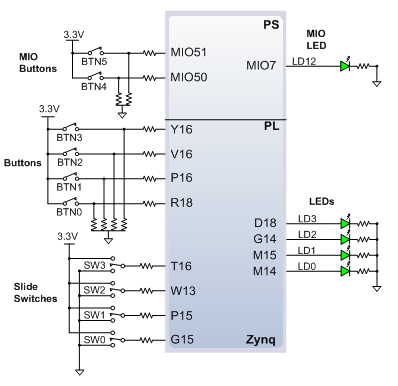
\includegraphics[width=0.55\textwidth]{src/png/digilent-zybo-ps-pl-gpio.png}
			\caption{Uspořádání připojení tlačítek, přepínačů a LED k~PS a PL pro vývojovou desku Digilent Zybo. \cite{digilent-zybo-reference-manual}}
			\label{fig:digilent-zybo-ps-pl-gpio}
		\end{figure}


		Před dalším pokračováním je možné design validovat ponocí příslušného tlačítka validace na horizontální ovládací liště. Pokud je již HW design vytvořen a nakonfigurován, je možné v~kartě \textit{Sources/Design Sources} vybrat vytvořený design a pomocí nabídky pravého tlačítka myši vybrat možnost \textit{Create HDL Wrapper}. V tomto kroku je opět prováděna validace designu. Pokud se v~designu vyskytují kritická upozornění, která jsou zobrazena například na obr. \ref{fig:zybo-xilinx-vivado-flow-24}, je stále možné pokračovat v~tvorbě konečného produktu.\par
		Po vytvoření \textit{HDL Wrapper} je možné v~menu \textit{Flow Navigator/Program and Debug} zvolit krok \textit{Generate Bitstream}. Pokud do tohoto kroku nebyla provedena syntéza ani implementace designu, objeví se hlášení, že je třeba tyto kroky provést, v~případě pokračování v~požadavku generování bitstreamu budou automaticky provedeny. V navazující nabídce možné vybrat, zda procesy budou probíhat lokálně či na vzdáleném serveru, nebo clusteru. Také je možné zvolit kolik výpočetních jader procesoru se bude podílet na prováděných úkolech. V~případě využití osobního počítače pro generaci bitstreamu (i předcházející syntézy a implementace) autor práce doporučuje používat méně než polovinu dostupných jader. Tato volba vychází z~experimentálního zjištění, že v~případě využití vyššího počtu jader může dojít k~neočekávané chybě a proces provádění úkolů bude bez udání jakékoli informace ukončen a proces syntézy, implementace a generace bitstreamu bude nutné spustit znovu. Ukázka nastavení procesu je zobrazena na obr. \ref{fig:zybo-xilinx-vivado-flow-29}.\par


		\begin{figure}[htbp!]
			\centering
			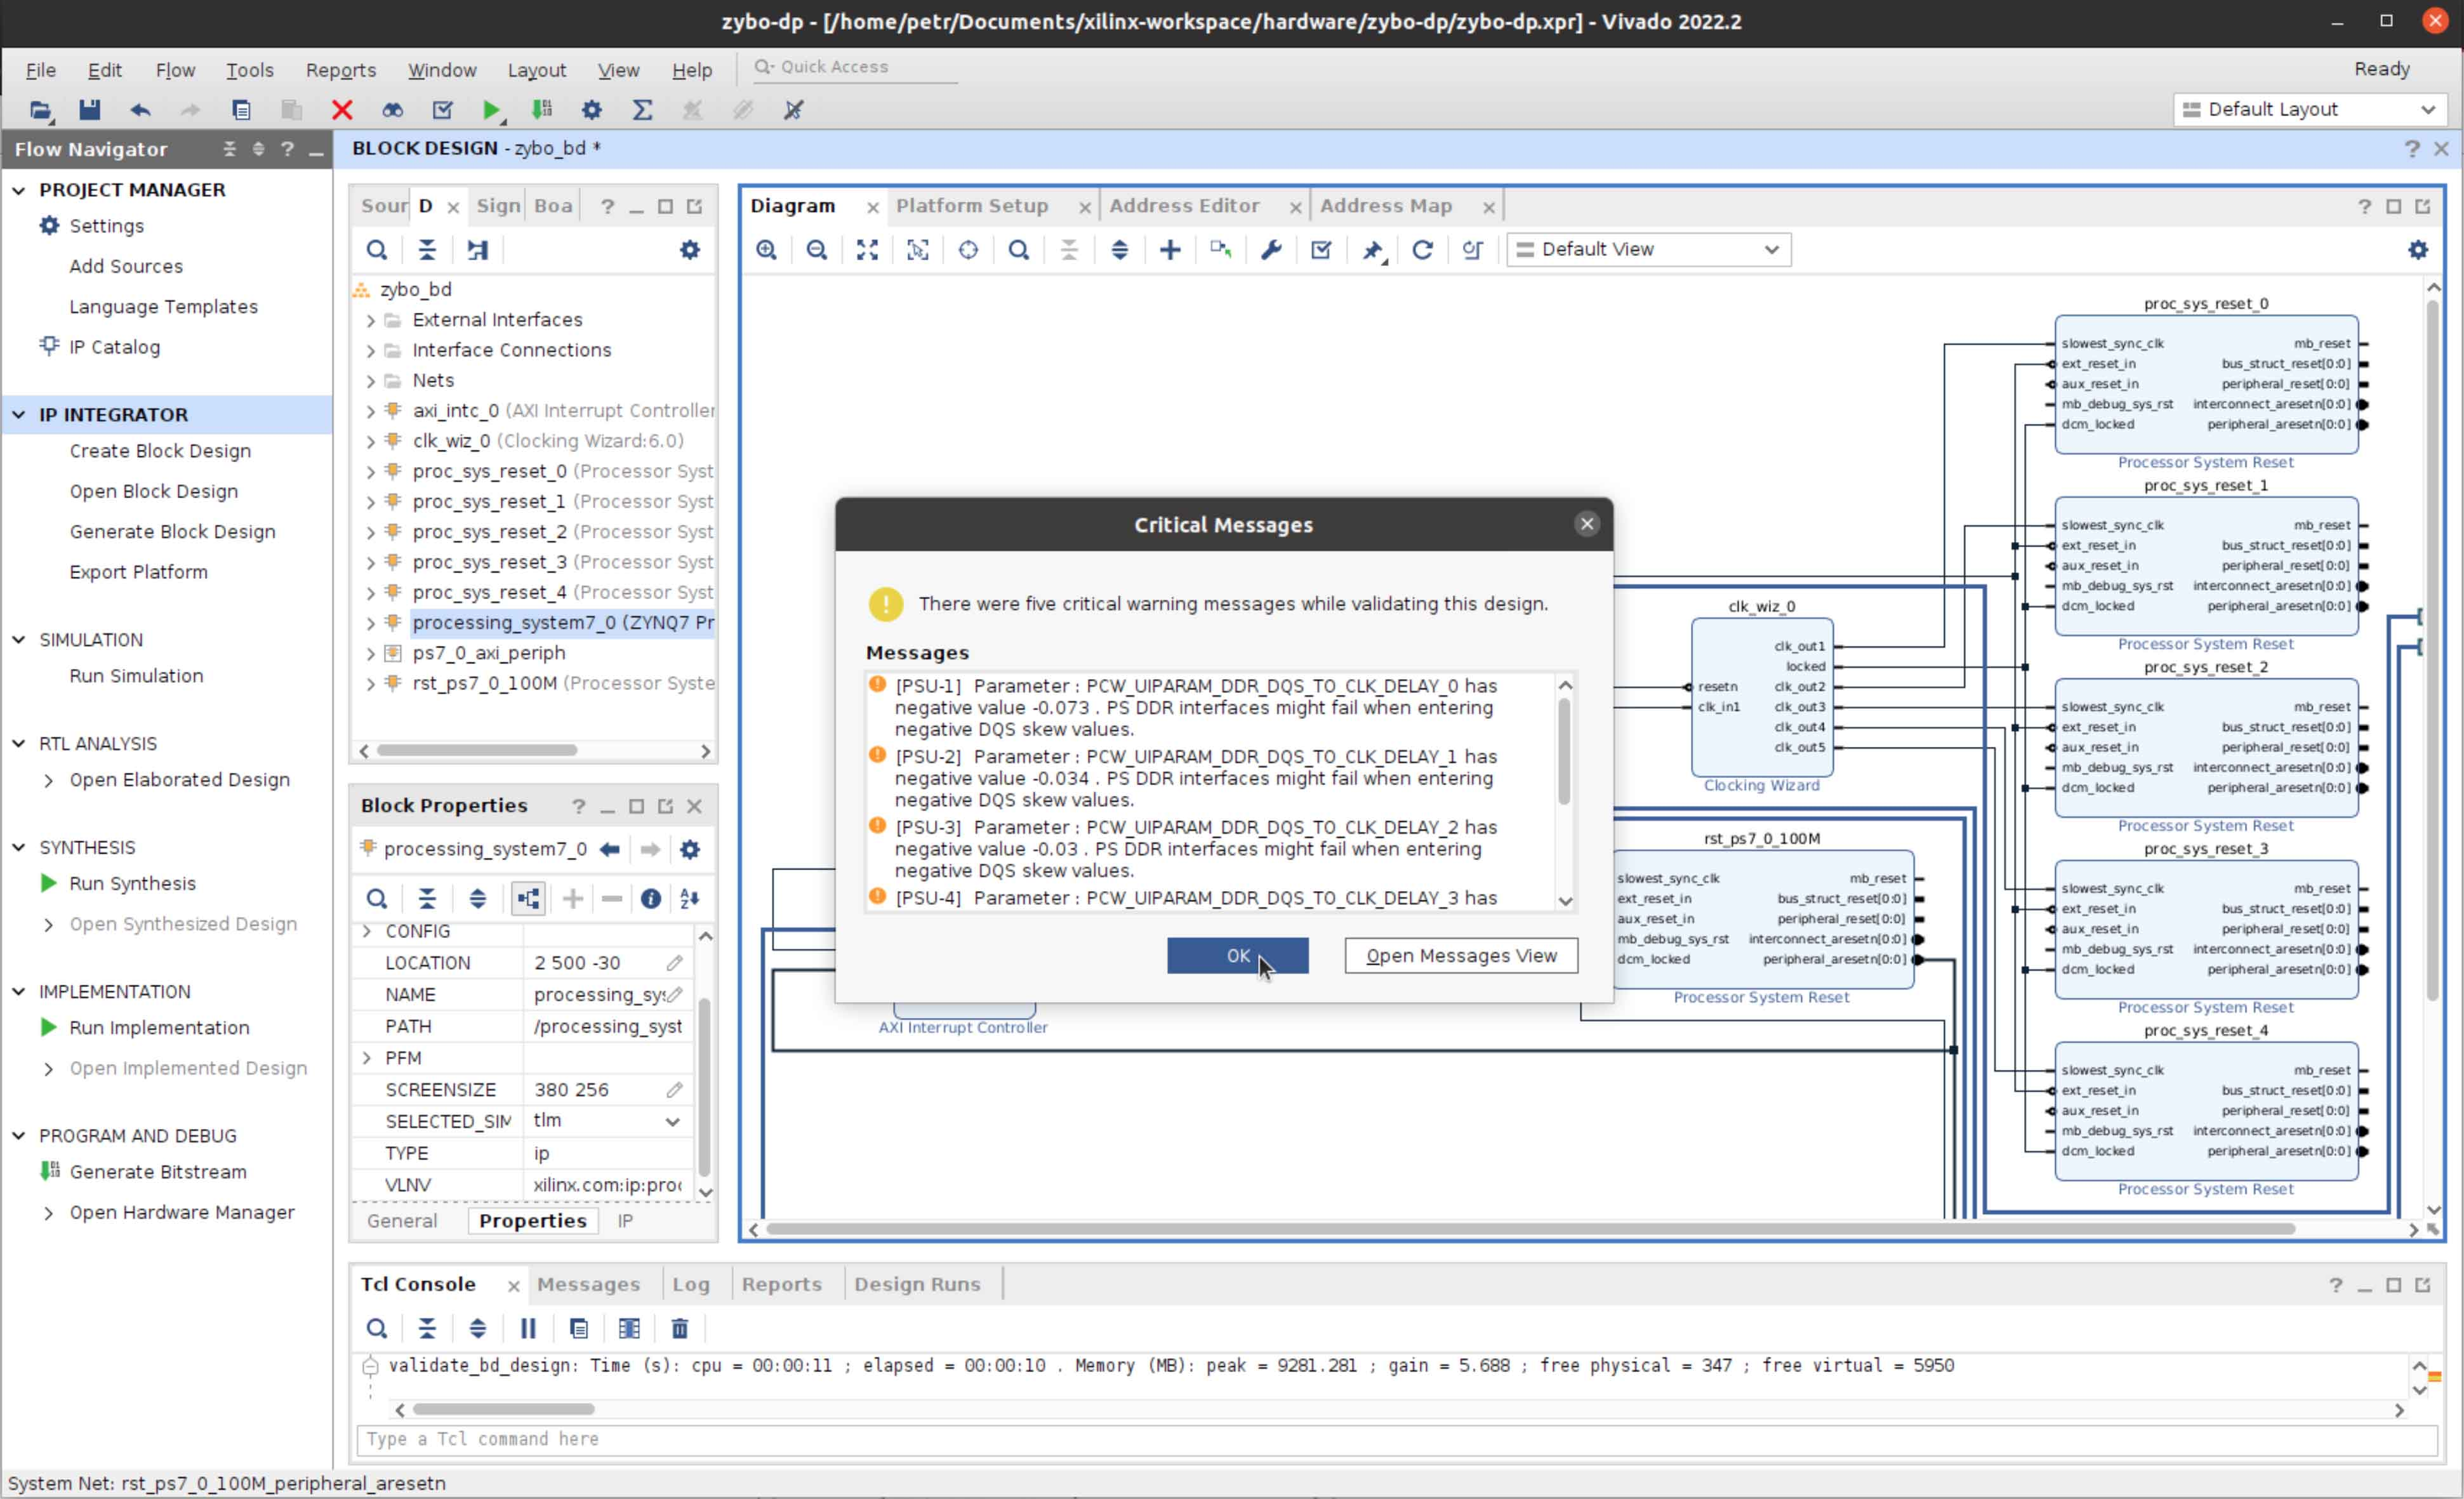
\includegraphics[width=0.85\textwidth]{src/png/zybo-xilinx-vivado-flow/zybo-xilinx-vivado-flow-24.jpg}
			\caption{Xilinx Vivado – kritická upozornění vzniklá po validaci designu, která je možné ignorovat.}
			\label{fig:zybo-xilinx-vivado-flow-24}
		\end{figure}


		\begin{figure}[htbp!]
			\centering
			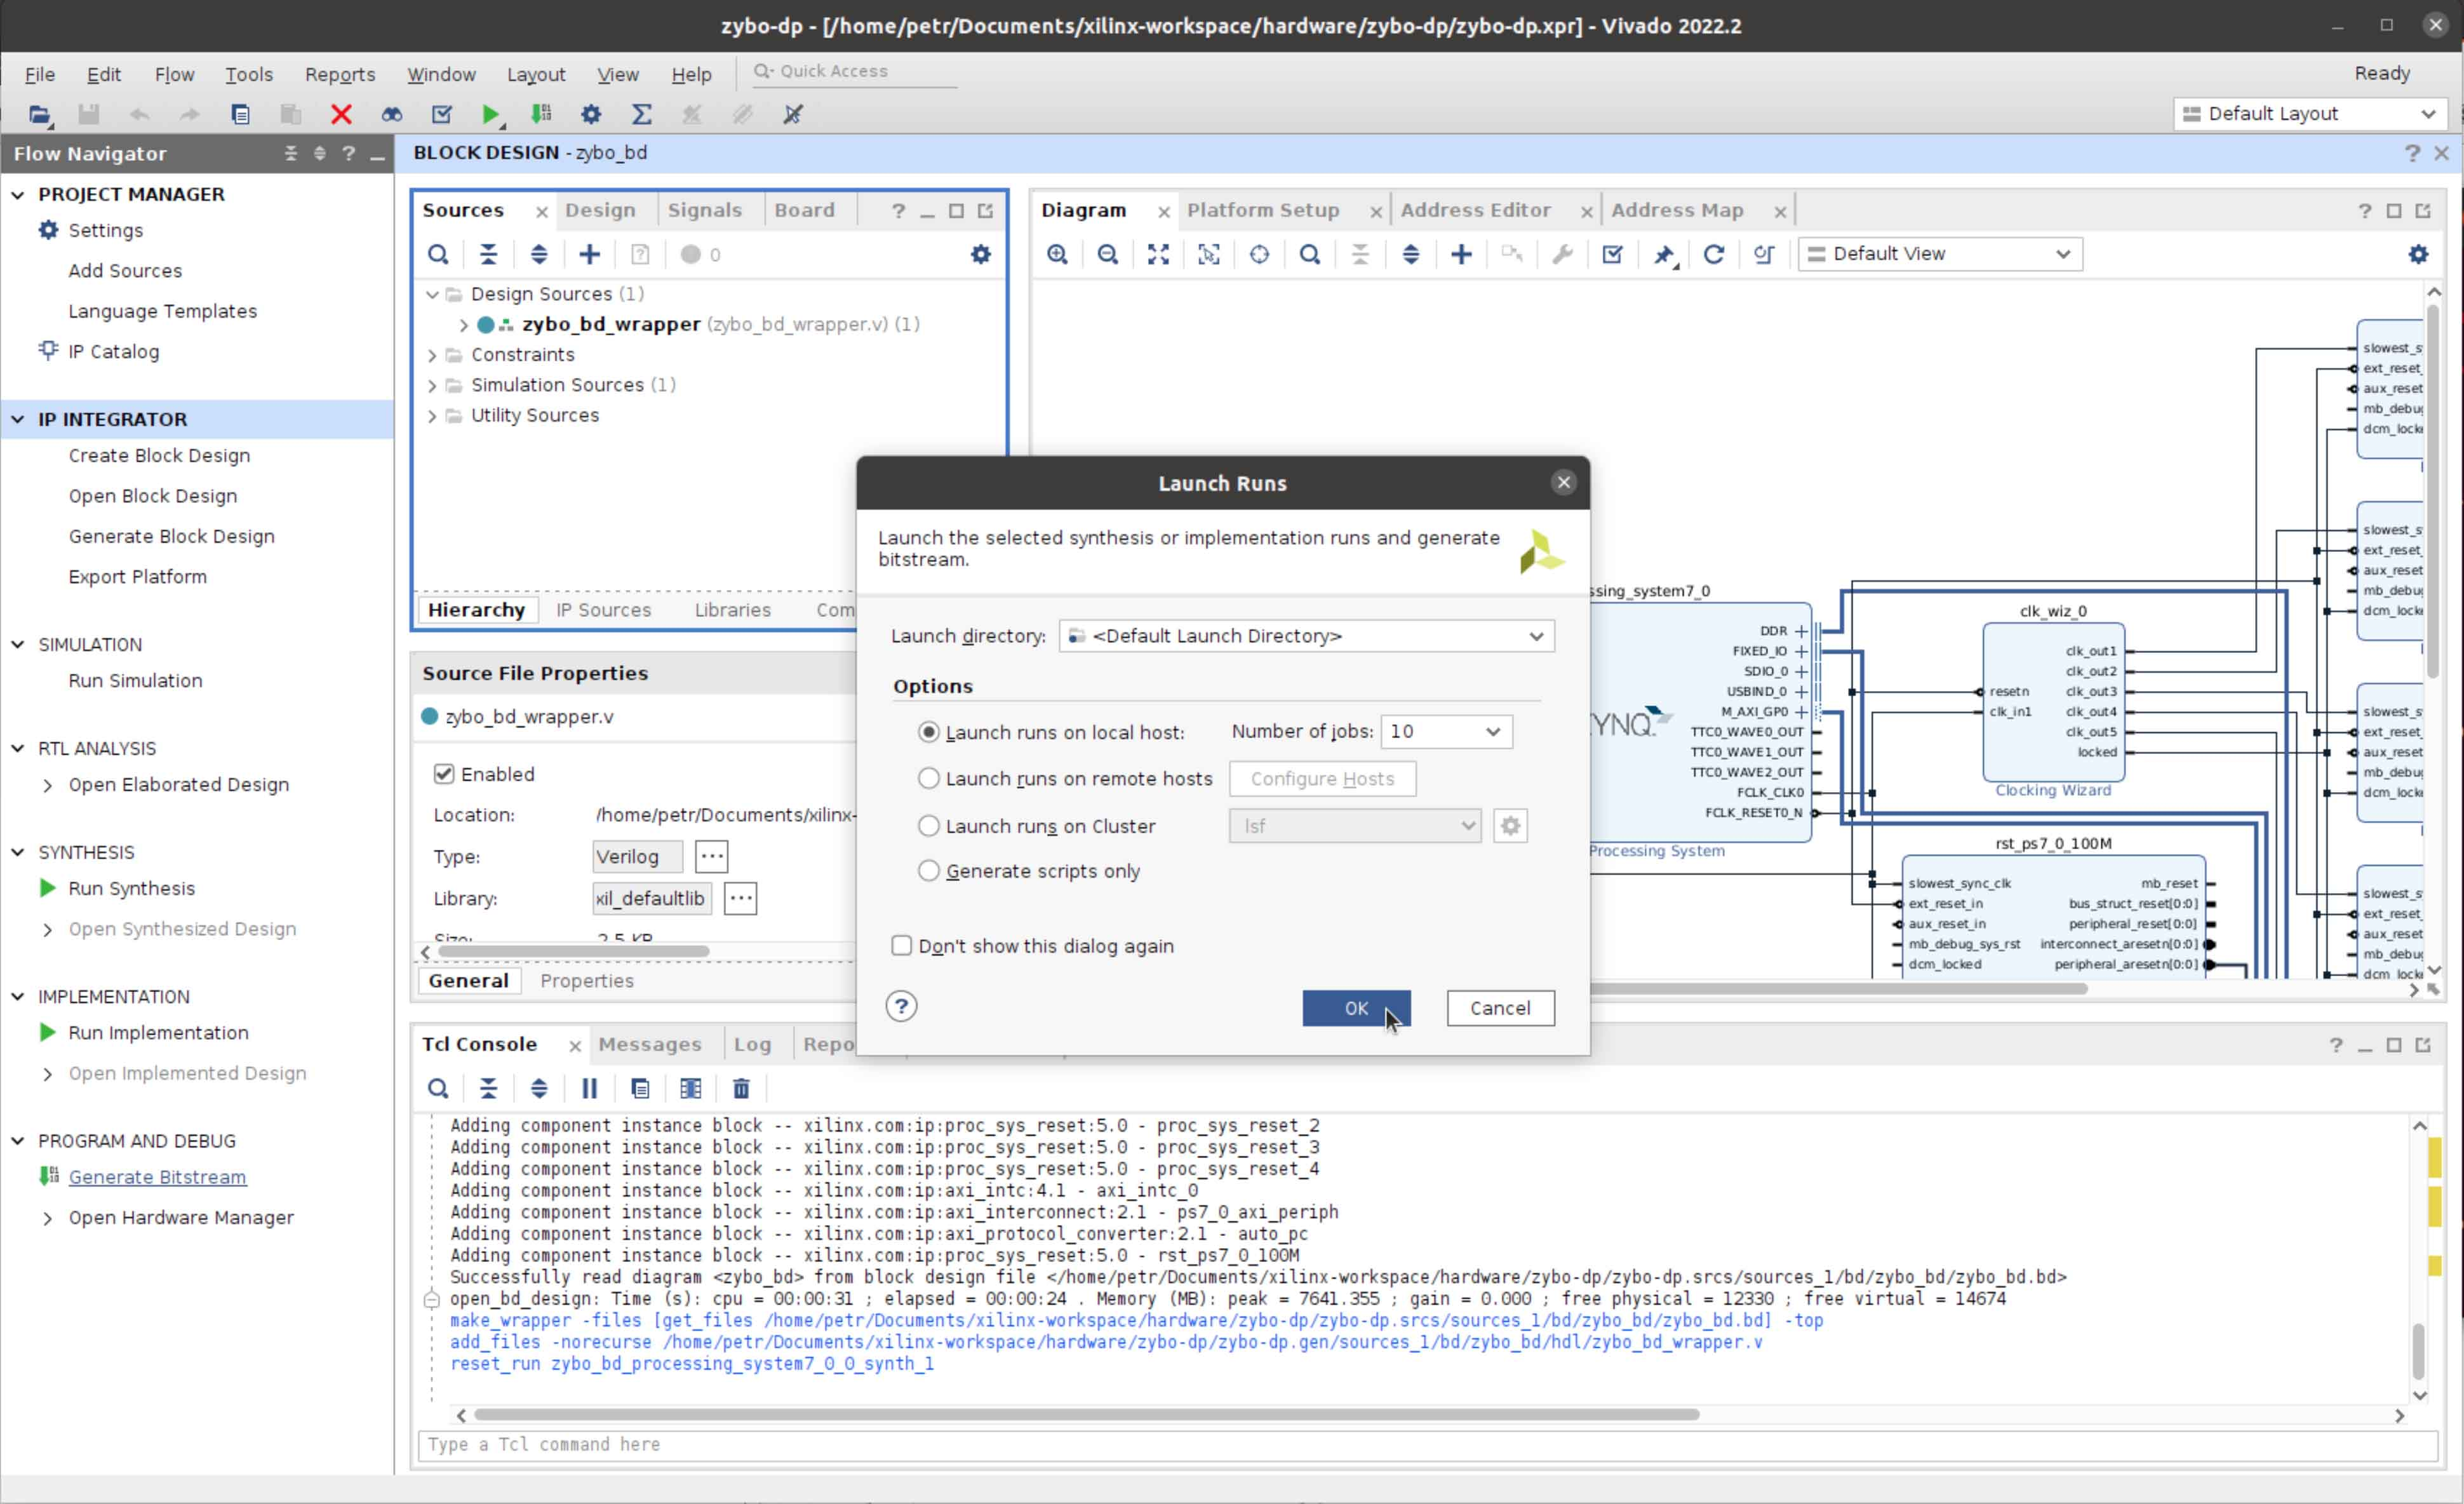
\includegraphics[width=0.85\textwidth]{src/png/zybo-xilinx-vivado-flow/zybo-xilinx-vivado-flow-29.jpg}
			\caption{Xilinx Vivado – nastavení provádění úkonů syntézy, implementace a generování bitstreamu, volba použitých výpočetních jader a určení, kde se mají procesy vykonávat pro Digilent Zybo.}
			\label{fig:zybo-xilinx-vivado-flow-29}
		\end{figure}

		Indikátor provádění jednotlivých procesů je umístěn v~pravém horním rohu. Záznam prováděných procesů je umístěn v~kartě \textit{Log}.\par
		Po úspěšném provedení jednotlivých kroků je zobrazena nabídka, která umožňuje nahlédnout na vytvořený design. Tuto nabídku je možné zavřít aniž by byla vykonávána jakákoliv z~nabízených možností.\par
		Po ukončení procesů je pro možné použití vytvořeného designu pro tvorbu PetaLinux systému a aplikací v~Xilinx Vitis nutné exportovat vytvořenou platformu. Export je proveden pomocí sekvence tlačítek \textit{File/Export/Export platform}. Ve výběru platformy je výhodné zvolit možnost \textit{Hardware and hardware emulation}, která umožňuje použít design pro skutečný HW i jeho emulaci. V~nabídce \textit{Platform State} je nutné vybrat možnost \textit{Pre-Synthesis}, která umožňuje další zpracování aplikace v~Xilinx Vitis pomocí V++. Důležitou volbou je zvolení možnost \textit{Include bistream}, který byl produktem tvorby designu v~této části.\par
		Po nastavení dodatečných informací platformy je možné jej vyexportovat do požadované lokace, kde bude dále využívána.
	\end{appendices}
\end{document}
